\documentclass[twoside]{book}

% Packages required by doxygen
\usepackage{calc}
\usepackage{doxygen}
\usepackage{graphicx}
\usepackage[utf8]{inputenc}
\usepackage{makeidx}
\usepackage{multicol}
\usepackage{multirow}
\usepackage{textcomp}
\usepackage[table]{xcolor}

% Font selection
\usepackage[T1]{fontenc}
\usepackage{mathptmx}
\usepackage[scaled=.90]{helvet}
\usepackage{courier}
\usepackage{amssymb}
\usepackage{sectsty}
\renewcommand{\familydefault}{\sfdefault}
\allsectionsfont{%
  \fontseries{bc}\selectfont%
  \color{darkgray}%
}
\renewcommand{\DoxyLabelFont}{%
  \fontseries{bc}\selectfont%
  \color{darkgray}%
}

% Page & text layout
\usepackage{geometry}
\geometry{%
  a4paper,%
  top=2.5cm,%
  bottom=2.5cm,%
  left=2.5cm,%
  right=2.5cm%
}
\tolerance=750
\hfuzz=15pt
\hbadness=750
\setlength{\emergencystretch}{15pt}
\setlength{\parindent}{0cm}
\setlength{\parskip}{0.2cm}
\makeatletter
\renewcommand{\paragraph}{%
  \@startsection{paragraph}{4}{0ex}{-1.0ex}{1.0ex}{%
    \normalfont\normalsize\bfseries\SS@parafont%
  }%
}
\renewcommand{\subparagraph}{%
  \@startsection{subparagraph}{5}{0ex}{-1.0ex}{1.0ex}{%
    \normalfont\normalsize\bfseries\SS@subparafont%
  }%
}
\makeatother

% Headers & footers
\usepackage{fancyhdr}
\pagestyle{fancyplain}
\fancyhead[LE]{\fancyplain{}{\bfseries\thepage}}
\fancyhead[CE]{\fancyplain{}{}}
\fancyhead[RE]{\fancyplain{}{\bfseries\leftmark}}
\fancyhead[LO]{\fancyplain{}{\bfseries\rightmark}}
\fancyhead[CO]{\fancyplain{}{}}
\fancyhead[RO]{\fancyplain{}{\bfseries\thepage}}
\fancyfoot[LE]{\fancyplain{}{}}
\fancyfoot[CE]{\fancyplain{}{}}
\fancyfoot[RE]{\fancyplain{}{\bfseries\scriptsize Generated on Wed Dec 9 2015 14\-:02\-:39 for R\-A\-P\-P Platform A\-P\-I by Doxygen }}
\fancyfoot[LO]{\fancyplain{}{\bfseries\scriptsize Generated on Wed Dec 9 2015 14\-:02\-:39 for R\-A\-P\-P Platform A\-P\-I by Doxygen }}
\fancyfoot[CO]{\fancyplain{}{}}
\fancyfoot[RO]{\fancyplain{}{}}
\renewcommand{\footrulewidth}{0.4pt}
\renewcommand{\chaptermark}[1]{%
  \markboth{#1}{}%
}
\renewcommand{\sectionmark}[1]{%
  \markright{\thesection\ #1}%
}

% Indices & bibliography
\usepackage{natbib}
\usepackage[titles]{tocloft}
\setcounter{tocdepth}{3}
\setcounter{secnumdepth}{5}
\makeindex

% Hyperlinks (required, but should be loaded last)
\usepackage{ifpdf}
\ifpdf
  \usepackage[pdftex,pagebackref=true]{hyperref}
\else
  \usepackage[ps2pdf,pagebackref=true]{hyperref}
\fi
\hypersetup{%
  colorlinks=true,%
  linkcolor=blue,%
  citecolor=blue,%
  unicode%
}

% Custom commands
\newcommand{\clearemptydoublepage}{%
  \newpage{\pagestyle{empty}\cleardoublepage}%
}


%===== C O N T E N T S =====

\begin{document}

% Titlepage & ToC
\hypersetup{pageanchor=false}
\pagenumbering{roman}
\begin{titlepage}
\vspace*{7cm}
\begin{center}%
{\Large R\-A\-P\-P Platform A\-P\-I }\\
\vspace*{1cm}
{\large Generated by Doxygen 1.8.6}\\
\vspace*{0.5cm}
{\small Wed Dec 9 2015 14:02:39}\\
\end{center}
\end{titlepage}
\clearemptydoublepage
\tableofcontents
\clearemptydoublepage
\pagenumbering{arabic}
\hypersetup{pageanchor=true}

%--- Begin generated contents ---
\chapter{Namespace Index}
\section{Namespace List}
Here is a list of all namespaces with brief descriptions\-:\begin{DoxyCompactList}
\item\contentsline{section}{\hyperlink{namespacecognitive__exercise}{cognitive\-\_\-exercise} }{\pageref{namespacecognitive__exercise}}{}
\item\contentsline{section}{\hyperlink{namespacecognitive__exercise__main}{cognitive\-\_\-exercise\-\_\-main} }{\pageref{namespacecognitive__exercise__main}}{}
\item\contentsline{section}{\hyperlink{namespacemysql__wrapper}{mysql\-\_\-wrapper} }{\pageref{namespacemysql__wrapper}}{}
\item\contentsline{section}{\hyperlink{namespacemysql__wrapper__main}{mysql\-\_\-wrapper\-\_\-main} }{\pageref{namespacemysql__wrapper__main}}{}
\item\contentsline{section}{\hyperlink{namespacerapp__audio__processing}{rapp\-\_\-audio\-\_\-processing} }{\pageref{namespacerapp__audio__processing}}{}
\item\contentsline{section}{\hyperlink{namespacerapp__audio__processing_1_1rapp__audio__processing}{rapp\-\_\-audio\-\_\-processing.\-rapp\-\_\-audio\-\_\-processing} }{\pageref{namespacerapp__audio__processing_1_1rapp__audio__processing}}{}
\item\contentsline{section}{\hyperlink{namespacerapp__audio__processing_1_1rapp__detect__silence}{rapp\-\_\-audio\-\_\-processing.\-rapp\-\_\-detect\-\_\-silence} }{\pageref{namespacerapp__audio__processing_1_1rapp__detect__silence}}{}
\item\contentsline{section}{\hyperlink{namespacerapp__audio__processing_1_1rapp__energy__denoise}{rapp\-\_\-audio\-\_\-processing.\-rapp\-\_\-energy\-\_\-denoise} }{\pageref{namespacerapp__audio__processing_1_1rapp__energy__denoise}}{}
\item\contentsline{section}{\hyperlink{namespacerapp__audio__processing_1_1rapp__set__noise__profile}{rapp\-\_\-audio\-\_\-processing.\-rapp\-\_\-set\-\_\-noise\-\_\-profile} }{\pageref{namespacerapp__audio__processing_1_1rapp__set__noise__profile}}{}
\item\contentsline{section}{\hyperlink{namespacerapp__audio__processing_1_1rapp__sox__denoise}{rapp\-\_\-audio\-\_\-processing.\-rapp\-\_\-sox\-\_\-denoise} }{\pageref{namespacerapp__audio__processing_1_1rapp__sox__denoise}}{}
\item\contentsline{section}{\hyperlink{namespacerapp__audio__processing_1_1rapp__transform__audio}{rapp\-\_\-audio\-\_\-processing.\-rapp\-\_\-transform\-\_\-audio} }{\pageref{namespacerapp__audio__processing_1_1rapp__transform__audio}}{}
\item\contentsline{section}{\hyperlink{namespacerapp__audio__processing_1_1rapp__utilities}{rapp\-\_\-audio\-\_\-processing.\-rapp\-\_\-utilities} }{\pageref{namespacerapp__audio__processing_1_1rapp__utilities}}{}
\item\contentsline{section}{\hyperlink{namespacerapp__exceptions}{rapp\-\_\-exceptions} }{\pageref{namespacerapp__exceptions}}{}
\item\contentsline{section}{\hyperlink{namespacerapp__speech__detection__sphinx4}{rapp\-\_\-speech\-\_\-detection\-\_\-sphinx4} }{\pageref{namespacerapp__speech__detection__sphinx4}}{}
\item\contentsline{section}{\hyperlink{namespacerapp__speech__detection__sphinx4_1_1english__support}{rapp\-\_\-speech\-\_\-detection\-\_\-sphinx4.\-english\-\_\-support} }{\pageref{namespacerapp__speech__detection__sphinx4_1_1english__support}}{}
\item\contentsline{section}{\hyperlink{namespacerapp__speech__detection__sphinx4_1_1global__parameters}{rapp\-\_\-speech\-\_\-detection\-\_\-sphinx4.\-global\-\_\-parameters} }{\pageref{namespacerapp__speech__detection__sphinx4_1_1global__parameters}}{}
\item\contentsline{section}{\hyperlink{namespacerapp__speech__detection__sphinx4_1_1greek__support}{rapp\-\_\-speech\-\_\-detection\-\_\-sphinx4.\-greek\-\_\-support} }{\pageref{namespacerapp__speech__detection__sphinx4_1_1greek__support}}{}
\item\contentsline{section}{\hyperlink{namespacerapp__speech__detection__sphinx4_1_1limited__vocabulary__creator}{rapp\-\_\-speech\-\_\-detection\-\_\-sphinx4.\-limited\-\_\-vocabulary\-\_\-creator} }{\pageref{namespacerapp__speech__detection__sphinx4_1_1limited__vocabulary__creator}}{}
\item\contentsline{section}{\hyperlink{namespacerapp__speech__detection__sphinx4_1_1rapp__exceptions}{rapp\-\_\-speech\-\_\-detection\-\_\-sphinx4.\-rapp\-\_\-exceptions} }{\pageref{namespacerapp__speech__detection__sphinx4_1_1rapp__exceptions}}{}
\item\contentsline{section}{\hyperlink{namespacerapp__speech__detection__sphinx4_1_1rapp__tools}{rapp\-\_\-speech\-\_\-detection\-\_\-sphinx4.\-rapp\-\_\-tools} }{\pageref{namespacerapp__speech__detection__sphinx4_1_1rapp__tools}}{}
\item\contentsline{section}{\hyperlink{namespacerapp__speech__detection__sphinx4_1_1speech__recognition__sphinx4}{rapp\-\_\-speech\-\_\-detection\-\_\-sphinx4.\-speech\-\_\-recognition\-\_\-sphinx4} }{\pageref{namespacerapp__speech__detection__sphinx4_1_1speech__recognition__sphinx4}}{}
\item\contentsline{section}{\hyperlink{namespacerapp__speech__detection__sphinx4_1_1speech__recognition__sphinx4__handler__node}{rapp\-\_\-speech\-\_\-detection\-\_\-sphinx4.\-speech\-\_\-recognition\-\_\-sphinx4\-\_\-handler\-\_\-node} }{\pageref{namespacerapp__speech__detection__sphinx4_1_1speech__recognition__sphinx4__handler__node}}{}
\item\contentsline{section}{\hyperlink{namespacerapp__speech__detection__sphinx4_1_1sphinx4__configuration__params}{rapp\-\_\-speech\-\_\-detection\-\_\-sphinx4.\-sphinx4\-\_\-configuration\-\_\-params} }{\pageref{namespacerapp__speech__detection__sphinx4_1_1sphinx4__configuration__params}}{}
\item\contentsline{section}{\hyperlink{namespacerapp__speech__detection__sphinx4_1_1sphinx4__wrapper}{rapp\-\_\-speech\-\_\-detection\-\_\-sphinx4.\-sphinx4\-\_\-wrapper} }{\pageref{namespacerapp__speech__detection__sphinx4_1_1sphinx4__wrapper}}{}
\item\contentsline{section}{\hyperlink{namespacespeech__recognition__google}{speech\-\_\-recognition\-\_\-google} }{\pageref{namespacespeech__recognition__google}}{}
\item\contentsline{section}{\hyperlink{namespacetext__to__speech__espeak}{text\-\_\-to\-\_\-speech\-\_\-espeak} }{\pageref{namespacetext__to__speech__espeak}}{}
\end{DoxyCompactList}

\chapter{Hierarchical Index}
\section{Class Hierarchy}
This inheritance list is sorted roughly, but not completely, alphabetically\-:\begin{DoxyCompactList}
\item Test\begin{DoxyCompactList}
\item \contentsline{section}{Door\-Check\-Test}{\pageref{classDoorCheckTest}}{}
\item \contentsline{section}{Light\-Check\-Test}{\pageref{classLightCheckTest}}{}
\end{DoxyCompactList}
\item Test\-Case\begin{DoxyCompactList}
\item \contentsline{section}{functional\-\_\-tests.\-Hazard\-Detection\-Func}{\pageref{classfunctional__tests_1_1HazardDetectionFunc}}{}
\end{DoxyCompactList}
\end{DoxyCompactList}

\chapter{Class Index}
\section{Class List}
Here are the classes, structs, unions and interfaces with brief descriptions\-:\begin{DoxyCompactList}
\item\contentsline{section}{\hyperlink{classgoogle__news__explorer__test_1_1TestGoogleNewsExplorer}{google\-\_\-news\-\_\-explorer\-\_\-test.\-Test\-Google\-News\-Explorer} }{\pageref{classgoogle__news__explorer__test_1_1TestGoogleNewsExplorer}}{}
\end{DoxyCompactList}

\chapter{File Index}
\section{File List}
Here is a list of all files with brief descriptions\-:\begin{DoxyCompactList}
\item\contentsline{section}{/home/travis/rapp\-\_\-temp/rapp-\/api/cpp/examples/\hyperlink{face__detect_8cpp}{face\-\_\-detect.\-cpp} }{\pageref{face__detect_8cpp}}{}
\item\contentsline{section}{/home/travis/rapp\-\_\-temp/rapp-\/api/cpp/examples/\hyperlink{fetch__data_8cpp}{fetch\-\_\-data.\-cpp} }{\pageref{fetch__data_8cpp}}{}
\item\contentsline{section}{/home/travis/rapp\-\_\-temp/rapp-\/api/cpp/examples/\hyperlink{ontology__example_8cpp}{ontology\-\_\-example.\-cpp} }{\pageref{ontology__example_8cpp}}{}
\item\contentsline{section}{/home/travis/rapp\-\_\-temp/rapp-\/api/cpp/examples/\hyperlink{picture__example_8cpp}{picture\-\_\-example.\-cpp} }{\pageref{picture__example_8cpp}}{}
\item\contentsline{section}{/home/travis/rapp\-\_\-temp/rapp-\/api/cpp/examples/\hyperlink{qr__detect_8cpp}{qr\-\_\-detect.\-cpp} }{\pageref{qr__detect_8cpp}}{}
\item\contentsline{section}{/home/travis/rapp\-\_\-temp/rapp-\/api/cpp/examples/\hyperlink{set__denoise__example_8cpp}{set\-\_\-denoise\-\_\-example.\-cpp} }{\pageref{set__denoise__example_8cpp}}{}
\item\contentsline{section}{/home/travis/rapp\-\_\-temp/rapp-\/api/cpp/examples/\hyperlink{speech__to__text_8cpp}{speech\-\_\-to\-\_\-text.\-cpp} }{\pageref{speech__to__text_8cpp}}{}
\item\contentsline{section}{/home/travis/rapp\-\_\-temp/rapp-\/api/cpp/includes/cloud/face\-Detector/\hyperlink{faceDetector_8hpp}{face\-Detector.\-hpp} }{\pageref{faceDetector_8hpp}}{}
\item\contentsline{section}{/home/travis/rapp\-\_\-temp/rapp-\/api/cpp/includes/cloud/face\-Detector/\hyperlink{cloud_2faceDetector_2Includes_8ihh}{Includes.\-ihh} }{\pageref{cloud_2faceDetector_2Includes_8ihh}}{}
\item\contentsline{section}{/home/travis/rapp\-\_\-temp/rapp-\/api/cpp/includes/cloud/fetch\-Personal\-Data/\hyperlink{fetchPersonalData_8hpp}{fetch\-Personal\-Data.\-hpp} }{\pageref{fetchPersonalData_8hpp}}{}
\item\contentsline{section}{/home/travis/rapp\-\_\-temp/rapp-\/api/cpp/includes/cloud/fetch\-Personal\-Data/\hyperlink{cloud_2fetchPersonalData_2Includes_8ihh}{Includes.\-ihh} }{\pageref{cloud_2fetchPersonalData_2Includes_8ihh}}{}
\item\contentsline{section}{/home/travis/rapp\-\_\-temp/rapp-\/api/cpp/includes/cloud/ontology\-Is\-Sub\-Super\-Class\-Of/\hyperlink{cloud_2ontologyIsSubSuperClassOf_2Includes_8ihh}{Includes.\-ihh} }{\pageref{cloud_2ontologyIsSubSuperClassOf_2Includes_8ihh}}{}
\item\contentsline{section}{/home/travis/rapp\-\_\-temp/rapp-\/api/cpp/includes/cloud/ontology\-Is\-Sub\-Super\-Class\-Of/\hyperlink{ontologyIsSubSuperClassOf_8hpp}{ontology\-Is\-Sub\-Super\-Class\-Of.\-hpp} }{\pageref{ontologyIsSubSuperClassOf_8hpp}}{}
\item\contentsline{section}{/home/travis/rapp\-\_\-temp/rapp-\/api/cpp/includes/cloud/ontology\-Sub\-Classes\-Of/\hyperlink{cloud_2ontologySubClassesOf_2Includes_8ihh}{Includes.\-ihh} }{\pageref{cloud_2ontologySubClassesOf_2Includes_8ihh}}{}
\item\contentsline{section}{/home/travis/rapp\-\_\-temp/rapp-\/api/cpp/includes/cloud/ontology\-Sub\-Classes\-Of/\hyperlink{ontologySubClassesOf_8hpp}{ontology\-Sub\-Classes\-Of.\-hpp} }{\pageref{ontologySubClassesOf_8hpp}}{}
\item\contentsline{section}{/home/travis/rapp\-\_\-temp/rapp-\/api/cpp/includes/cloud/ontology\-Super\-Classes\-Of/\hyperlink{cloud_2ontologySuperClassesOf_2Includes_8ihh}{Includes.\-ihh} }{\pageref{cloud_2ontologySuperClassesOf_2Includes_8ihh}}{}
\item\contentsline{section}{/home/travis/rapp\-\_\-temp/rapp-\/api/cpp/includes/cloud/ontology\-Super\-Classes\-Of/\hyperlink{ontologySuperClassesOf_8hpp}{ontology\-Super\-Classes\-Of.\-hpp} }{\pageref{ontologySuperClassesOf_8hpp}}{}
\item\contentsline{section}{/home/travis/rapp\-\_\-temp/rapp-\/api/cpp/includes/cloud/qr\-Detector/\hyperlink{cloud_2qrDetector_2Includes_8ihh}{Includes.\-ihh} }{\pageref{cloud_2qrDetector_2Includes_8ihh}}{}
\item\contentsline{section}{/home/travis/rapp\-\_\-temp/rapp-\/api/cpp/includes/cloud/qr\-Detector/\hyperlink{qrDetector_8hpp}{qr\-Detector.\-hpp} }{\pageref{qrDetector_8hpp}}{}
\item\contentsline{section}{/home/travis/rapp\-\_\-temp/rapp-\/api/cpp/includes/cloud/set\-Denoise\-Profile/\hyperlink{cloud_2setDenoiseProfile_2Includes_8ihh}{Includes.\-ihh} }{\pageref{cloud_2setDenoiseProfile_2Includes_8ihh}}{}
\item\contentsline{section}{/home/travis/rapp\-\_\-temp/rapp-\/api/cpp/includes/cloud/set\-Denoise\-Profile/\hyperlink{setDenoiseProfile_8hpp}{set\-Denoise\-Profile.\-hpp} }{\pageref{setDenoiseProfile_8hpp}}{}
\item\contentsline{section}{/home/travis/rapp\-\_\-temp/rapp-\/api/cpp/includes/cloud/speech\-To\-Text/\hyperlink{cloud_2speechToText_2Includes_8ihh}{Includes.\-ihh} }{\pageref{cloud_2speechToText_2Includes_8ihh}}{}
\item\contentsline{section}{/home/travis/rapp\-\_\-temp/rapp-\/api/cpp/includes/cloud/speech\-To\-Text/\hyperlink{speechToText_8hpp}{speech\-To\-Text.\-hpp} }{\pageref{speechToText_8hpp}}{}
\item\contentsline{section}{/home/travis/rapp\-\_\-temp/rapp-\/api/cpp/includes/cloud/up\-Services/\hyperlink{cloud_2upServices_2Includes_8ihh}{Includes.\-ihh} }{\pageref{cloud_2upServices_2Includes_8ihh}}{}
\item\contentsline{section}{/home/travis/rapp\-\_\-temp/rapp-\/api/cpp/includes/cloud/up\-Services/\hyperlink{upServices_8hpp}{up\-Services.\-hpp} }{\pageref{upServices_8hpp}}{}
\item\contentsline{section}{/home/travis/rapp\-\_\-temp/rapp-\/api/cpp/includes/objects/audio/\hyperlink{audio_8hpp}{audio.\-hpp} }{\pageref{audio_8hpp}}{}
\item\contentsline{section}{/home/travis/rapp\-\_\-temp/rapp-\/api/cpp/includes/objects/audio/\hyperlink{objects_2audio_2Includes_8ihh}{Includes.\-ihh} }{\pageref{objects_2audio_2Includes_8ihh}}{}
\item\contentsline{section}{/home/travis/rapp\-\_\-temp/rapp-\/api/cpp/includes/objects/face/\hyperlink{face_8hpp}{face.\-hpp} }{\pageref{face_8hpp}}{}
\item\contentsline{section}{/home/travis/rapp\-\_\-temp/rapp-\/api/cpp/includes/objects/face/\hyperlink{objects_2face_2Includes_8ihh}{Includes.\-ihh} }{\pageref{objects_2face_2Includes_8ihh}}{}
\item\contentsline{section}{/home/travis/rapp\-\_\-temp/rapp-\/api/cpp/includes/objects/picture/\hyperlink{objects_2picture_2Includes_8ihh}{Includes.\-ihh} }{\pageref{objects_2picture_2Includes_8ihh}}{}
\item\contentsline{section}{/home/travis/rapp\-\_\-temp/rapp-\/api/cpp/includes/objects/picture/\hyperlink{picture_8hpp}{picture.\-hpp} }{\pageref{picture_8hpp}}{}
\item\contentsline{section}{/home/travis/rapp\-\_\-temp/rapp-\/api/cpp/includes/objects/qr\-Code/\hyperlink{objects_2qrCode_2Includes_8ihh}{Includes.\-ihh} }{\pageref{objects_2qrCode_2Includes_8ihh}}{}
\item\contentsline{section}{/home/travis/rapp\-\_\-temp/rapp-\/api/cpp/includes/objects/qr\-Code/\hyperlink{qrCode_8hpp}{qr\-Code.\-hpp} }{\pageref{qrCode_8hpp}}{}
\item\contentsline{section}{/home/travis/rapp\-\_\-temp/rapp-\/api/cpp/includes/robot/communication/\hyperlink{communication_8hpp}{communication.\-hpp} }{\pageref{communication_8hpp}}{}
\item\contentsline{section}{/home/travis/rapp\-\_\-temp/rapp-\/api/cpp/includes/robot/communication/\hyperlink{robot_2communication_2Includes_8ihh}{Includes.\-ihh} }{\pageref{robot_2communication_2Includes_8ihh}}{}
\item\contentsline{section}{/home/travis/rapp\-\_\-temp/rapp-\/api/cpp/includes/robot/nao/\hyperlink{robot_2nao_2Includes_8ihh}{Includes.\-ihh} }{\pageref{robot_2nao_2Includes_8ihh}}{}
\item\contentsline{section}{/home/travis/rapp\-\_\-temp/rapp-\/api/cpp/includes/robot/nao/\hyperlink{nao_8hpp}{nao.\-hpp} }{\pageref{nao_8hpp}}{}
\item\contentsline{section}{/home/travis/rapp\-\_\-temp/rapp-\/api/cpp/includes/robot/navigation/\hyperlink{robot_2navigation_2Includes_8ihh}{Includes.\-ihh} }{\pageref{robot_2navigation_2Includes_8ihh}}{}
\item\contentsline{section}{/home/travis/rapp\-\_\-temp/rapp-\/api/cpp/includes/robot/navigation/\hyperlink{navigation_8hpp}{navigation.\-hpp} }{\pageref{navigation_8hpp}}{}
\item\contentsline{section}{/home/travis/rapp\-\_\-temp/rapp-\/api/cpp/includes/robot/proto/\hyperlink{robot_2proto_2Includes_8ihh}{Includes.\-ihh} }{\pageref{robot_2proto_2Includes_8ihh}}{}
\item\contentsline{section}{/home/travis/rapp\-\_\-temp/rapp-\/api/cpp/includes/robot/proto/\hyperlink{proto_8hpp}{proto.\-hpp} }{\pageref{proto_8hpp}}{}
\item\contentsline{section}{/home/travis/rapp\-\_\-temp/rapp-\/api/cpp/includes/robot/vision/\hyperlink{robot_2vision_2Includes_8ihh}{Includes.\-ihh} }{\pageref{robot_2vision_2Includes_8ihh}}{}
\item\contentsline{section}{/home/travis/rapp\-\_\-temp/rapp-\/api/cpp/includes/robot/vision/\hyperlink{vision_8hpp}{vision.\-hpp} }{\pageref{vision_8hpp}}{}
\item\contentsline{section}{/home/travis/rapp\-\_\-temp/rapp-\/api/cpp/includes/service/asio\-\_\-service\-\_\-http/\hyperlink{asio__service__http_8hpp}{asio\-\_\-service\-\_\-http.\-hpp} }{\pageref{asio__service__http_8hpp}}{}
\item\contentsline{section}{/home/travis/rapp\-\_\-temp/rapp-\/api/cpp/includes/service/asio\-\_\-service\-\_\-http/\hyperlink{service_2asio__service__http_2Includes_8ihh}{Includes.\-ihh} }{\pageref{service_2asio__service__http_2Includes_8ihh}}{}
\item\contentsline{section}{/home/travis/rapp\-\_\-temp/rapp-\/api/cpp/includes/service/asio\-\_\-service\-\_\-raw/\hyperlink{asio__service__raw_8cpp}{asio\-\_\-service\-\_\-raw.\-cpp} }{\pageref{asio__service__raw_8cpp}}{}
\item\contentsline{section}{/home/travis/rapp\-\_\-temp/rapp-\/api/cpp/includes/service/asio\-\_\-service\-\_\-raw/\hyperlink{asio__service__raw_8hpp}{asio\-\_\-service\-\_\-raw.\-hpp} }{\pageref{asio__service__raw_8hpp}}{}
\item\contentsline{section}{/home/travis/rapp\-\_\-temp/rapp-\/api/cpp/includes/service/asio\-\_\-service\-\_\-raw/\hyperlink{service_2asio__service__raw_2Includes_8ihh}{Includes.\-ihh} }{\pageref{service_2asio__service__raw_2Includes_8ihh}}{}
\item\contentsline{section}{/home/travis/rapp\-\_\-temp/rapp-\/api/cpp/includes/service/asio\-\_\-socket/\hyperlink{asio__socket_8hpp}{asio\-\_\-socket.\-hpp} }{\pageref{asio__socket_8hpp}}{}
\item\contentsline{section}{/home/travis/rapp\-\_\-temp/rapp-\/api/cpp/includes/service/asio\-\_\-socket/\hyperlink{service_2asio__socket_2Includes_8ihh}{Includes.\-ihh} }{\pageref{service_2asio__socket_2Includes_8ihh}}{}
\item\contentsline{section}{/home/travis/rapp\-\_\-temp/rapp-\/api/cpp/includes/service/globals/\hyperlink{globals_8hpp}{globals.\-hpp} }{\pageref{globals_8hpp}}{}
\item\contentsline{section}{/home/travis/rapp\-\_\-temp/rapp-\/api/cpp/includes/service/service\-\_\-controller/\hyperlink{service_2service__controller_2Includes_8ihh}{Includes.\-ihh} }{\pageref{service_2service__controller_2Includes_8ihh}}{}
\item\contentsline{section}{/home/travis/rapp\-\_\-temp/rapp-\/api/cpp/includes/service/service\-\_\-controller/\hyperlink{service__controller_8hpp}{service\-\_\-controller.\-hpp} }{\pageref{service__controller_8hpp}}{}
\item\contentsline{section}{/home/travis/rapp\-\_\-temp/rapp-\/api/python/\-Rapp\-Cloud/\hyperlink{____init_____8py}{\-\_\-\-\_\-init\-\_\-\-\_\-.\-py} }{\pageref{____init_____8py}}{}
\item\contentsline{section}{/home/travis/rapp\-\_\-temp/rapp-\/api/python/\-Rapp\-Cloud/\hyperlink{RappCloud_8py}{Rapp\-Cloud.\-py} }{\pageref{RappCloud_8py}}{}
\item\contentsline{section}{/home/travis/rapp\-\_\-temp/rapp-\/api/python/\-Rapp\-Cloud/\-Cloud\-Interface/\hyperlink{CloudInterface_2____init_____8py}{\-\_\-\-\_\-init\-\_\-\-\_\-.\-py} }{\pageref{CloudInterface_2____init_____8py}}{}
\item\contentsline{section}{/home/travis/rapp\-\_\-temp/rapp-\/api/python/\-Rapp\-Cloud/\-Cloud\-Interface/\hyperlink{CloudInterface_8py}{Cloud\-Interface.\-py} }{\pageref{CloudInterface_8py}}{}
\item\contentsline{section}{/home/travis/rapp\-\_\-temp/rapp-\/api/python/\-Rapp\-Cloud/\-Rand\-Str\-Gen/\hyperlink{RandStrGen_2____init_____8py}{\-\_\-\-\_\-init\-\_\-\-\_\-.\-py} }{\pageref{RandStrGen_2____init_____8py}}{}
\item\contentsline{section}{/home/travis/rapp\-\_\-temp/rapp-\/api/python/\-Rapp\-Cloud/\-Rand\-Str\-Gen/\hyperlink{RandStrGen_8py}{Rand\-Str\-Gen.\-py} }{\pageref{RandStrGen_8py}}{}
\end{DoxyCompactList}

\chapter{Namespace Documentation}
\hypertarget{namespacerapp}{\section{rapp Namespace Reference}
\label{namespacerapp}\index{rapp@{rapp}}
}
\subsection*{Namespaces}
\begin{DoxyCompactItemize}
\item 
\hyperlink{namespacerapp_1_1cloud}{cloud}
\item 
\hyperlink{namespacerapp_1_1object}{object}
\item 
\hyperlink{namespacerapp_1_1types}{types}
\begin{DoxyCompactList}\small\item\em Common global types. \end{DoxyCompactList}\end{DoxyCompactItemize}

\hypertarget{namespacerapp_1_1cloud}{\section{rapp\-:\-:cloud Namespace Reference}
\label{namespacerapp_1_1cloud}\index{rapp\-::cloud@{rapp\-::cloud}}
}
\subsection*{Classes}
\begin{DoxyCompactItemize}
\item 
class \hyperlink{classrapp_1_1cloud_1_1asio__handler}{asio\-\_\-handler}
\begin{DoxyCompactList}\small\item\em base class for asio handling, including helper methods and most protected members \end{DoxyCompactList}\item 
class \hyperlink{classrapp_1_1cloud_1_1asio__service__http}{asio\-\_\-service\-\_\-http}
\begin{DoxyCompactList}\small\item\em base class for asynchronous http websockets used for connecting to cloud services \end{DoxyCompactList}\item 
class \hyperlink{classrapp_1_1cloud_1_1asio__socket}{asio\-\_\-socket}
\begin{DoxyCompactList}\small\item\em Abstract Base A\-S\-I\-O Socket class Use for passing around to the service controller, various types of cloud handlers. This Interface is needed so that different handlers can be passed to the scheduler transparently. \end{DoxyCompactList}\item 
class \hyperlink{classrapp_1_1cloud_1_1asio__socket__https}{asio\-\_\-socket\-\_\-https}
\begin{DoxyCompactList}\small\item\em wrapper for S\-S\-L/\-T\-L\-S secure H\-T\-T\-P communication \end{DoxyCompactList}\item 
class \hyperlink{classrapp_1_1cloud_1_1available__services}{available\-\_\-services}
\begin{DoxyCompactList}\small\item\em requests available services from platform \end{DoxyCompactList}\item 
class \hyperlink{classrapp_1_1cloud_1_1cognitive__get__history}{cognitive\-\_\-get\-\_\-history}
\item 
class \hyperlink{classrapp_1_1cloud_1_1cognitive__get__scores}{cognitive\-\_\-get\-\_\-scores}
\item 
class \hyperlink{classrapp_1_1cloud_1_1cognitive__record__performance}{cognitive\-\_\-record\-\_\-performance}
\item 
class \hyperlink{classrapp_1_1cloud_1_1cognitive__test__selector}{cognitive\-\_\-test\-\_\-selector}
\begin{DoxyCompactList}\small\item\em chose a congitive game to play \end{DoxyCompactList}\item 
class \hyperlink{classrapp_1_1cloud_1_1email__fetch}{email\-\_\-fetch}
\begin{DoxyCompactList}\small\item\em fetch email(s) \end{DoxyCompactList}\item 
class \hyperlink{classrapp_1_1cloud_1_1email__send}{email\-\_\-send}
\begin{DoxyCompactList}\small\item\em send an email \end{DoxyCompactList}\item 
class \hyperlink{classrapp_1_1cloud_1_1face__detection}{face\-\_\-detection}
\begin{DoxyCompactList}\small\item\em Asynchronous Service which will request the cloud to detect faces. \end{DoxyCompactList}\item 
class \hyperlink{classrapp_1_1cloud_1_1fetch__personal__data}{fetch\-\_\-personal\-\_\-data}
\begin{DoxyCompactList}\small\item\em Get all personal data for a specific user. \end{DoxyCompactList}\item 
class \hyperlink{classrapp_1_1cloud_1_1geolocation}{geolocation}
\begin{DoxyCompactList}\small\item\em geolocation service \end{DoxyCompactList}\item 
class \hyperlink{classrapp_1_1cloud_1_1hazard__detection__door__check}{hazard\-\_\-detection\-\_\-door\-\_\-check}
\begin{DoxyCompactList}\small\item\em detect open doors \end{DoxyCompactList}\item 
class \hyperlink{classrapp_1_1cloud_1_1hazard__detection__light__check}{hazard\-\_\-detection\-\_\-light\-\_\-check}
\begin{DoxyCompactList}\small\item\em detect light levels \end{DoxyCompactList}\item 
class \hyperlink{classrapp_1_1cloud_1_1human__detection}{human\-\_\-detection}
\begin{DoxyCompactList}\small\item\em detect humans in an image \end{DoxyCompactList}\item 
class \hyperlink{classrapp_1_1cloud_1_1login__user}{login\-\_\-user}
\item 
class \hyperlink{classrapp_1_1cloud_1_1news__explore}{news\-\_\-explore}
\begin{DoxyCompactList}\small\item\em get news \end{DoxyCompactList}\item 
class \hyperlink{classrapp_1_1cloud_1_1object__recognition}{object\-\_\-recognition}
\begin{DoxyCompactList}\small\item\em recognize object from an image \end{DoxyCompactList}\item 
class \hyperlink{classrapp_1_1cloud_1_1ontology__is__subsuperclass__of}{ontology\-\_\-is\-\_\-subsuperclass\-\_\-of}
\begin{DoxyCompactList}\small\item\em query if sub class is a super class of param \end{DoxyCompactList}\item 
class \hyperlink{classrapp_1_1cloud_1_1ontology__subclasses__of}{ontology\-\_\-subclasses\-\_\-of}
\begin{DoxyCompactList}\small\item\em get ontology subclass of a query \end{DoxyCompactList}\item 
class \hyperlink{classrapp_1_1cloud_1_1ontology__superclasses__of}{ontology\-\_\-superclasses\-\_\-of}
\begin{DoxyCompactList}\small\item\em get ontology super-\/classes of query \end{DoxyCompactList}\item 
class \hyperlink{classrapp_1_1cloud_1_1path__upload__map}{path\-\_\-upload\-\_\-map}
\item 
class \hyperlink{classrapp_1_1cloud_1_1plan__path__2d}{plan\-\_\-path\-\_\-2d}
\item 
class \hyperlink{classrapp_1_1cloud_1_1qr__detection}{qr\-\_\-detection}
\begin{DoxyCompactList}\small\item\em Asynchronous Service which will request the cloud to detect Q\-R codes. \end{DoxyCompactList}\item 
class \hyperlink{classrapp_1_1cloud_1_1service__controller}{service\-\_\-controller}
\begin{DoxyCompactList}\small\item\em Main class that controllers R\-A\-P\-P Services. \end{DoxyCompactList}\item 
class \hyperlink{classrapp_1_1cloud_1_1set__denoise__profile}{set\-\_\-denoise\-\_\-profile}
\begin{DoxyCompactList}\small\item\em setting the denoising audio profile for speech recognition \end{DoxyCompactList}\item 
class \hyperlink{classrapp_1_1cloud_1_1speech__detection__google}{speech\-\_\-detection\-\_\-google}
\begin{DoxyCompactList}\small\item\em delegate speech-\/to-\/text to Google via R\-A\-P\-P \end{DoxyCompactList}\item 
class \hyperlink{classrapp_1_1cloud_1_1speech__detection__sphinx4}{speech\-\_\-detection\-\_\-sphinx4}
\begin{DoxyCompactList}\small\item\em speech-\/to-\/text recognition using C\-M\-U sphinx4 \end{DoxyCompactList}\item 
class \hyperlink{classrapp_1_1cloud_1_1text__to__speech}{text\-\_\-to\-\_\-speech}
\begin{DoxyCompactList}\small\item\em request speech audio from text \end{DoxyCompactList}\item 
class \hyperlink{classrapp_1_1cloud_1_1weather__report__current}{weather\-\_\-report\-\_\-current}
\begin{DoxyCompactList}\small\item\em get current weather report \end{DoxyCompactList}\item 
class \hyperlink{classrapp_1_1cloud_1_1weather__report__forecast}{weather\-\_\-report\-\_\-forecast}
\begin{DoxyCompactList}\small\item\em get weather forecast \end{DoxyCompactList}\end{DoxyCompactItemize}
\subsection*{Variables}
\begin{DoxyCompactItemize}
\item 
constexpr char \hyperlink{namespacerapp_1_1cloud_afb654734a7584ea0243e431aaebd4728}{address} \mbox{[}$\,$\mbox{]} = \char`\"{}localhost\char`\"{}
\begin{DoxyCompactList}\small\item\em api.\-rapp.\-cloud -\/ \end{DoxyCompactList}\item 
constexpr char \hyperlink{namespacerapp_1_1cloud_ae0e4cb6fd54bbf45234fc3c21f752b7a}{port} \mbox{[}$\,$\mbox{]} = \char`\"{}9001\char`\"{}
\begin{DoxyCompactList}\small\item\em api.\-rapp.\-cloud -\/ H\-O\-P server port \end{DoxyCompactList}\end{DoxyCompactItemize}


\subsection{Variable Documentation}
\hypertarget{namespacerapp_1_1cloud_afb654734a7584ea0243e431aaebd4728}{\index{rapp\-::cloud@{rapp\-::cloud}!address@{address}}
\index{address@{address}!rapp::cloud@{rapp\-::cloud}}
\subsubsection[{address}]{\setlength{\rightskip}{0pt plus 5cm}constexpr char rapp\-::cloud\-::address\mbox{[}$\,$\mbox{]} = \char`\"{}localhost\char`\"{}}}\label{namespacerapp_1_1cloud_afb654734a7584ea0243e431aaebd4728}


api.\-rapp.\-cloud -\/ 



Definition at line 8 of file asio\-\_\-socket.\-hpp.

\hypertarget{namespacerapp_1_1cloud_ae0e4cb6fd54bbf45234fc3c21f752b7a}{\index{rapp\-::cloud@{rapp\-::cloud}!port@{port}}
\index{port@{port}!rapp::cloud@{rapp\-::cloud}}
\subsubsection[{port}]{\setlength{\rightskip}{0pt plus 5cm}constexpr char rapp\-::cloud\-::port\mbox{[}$\,$\mbox{]} = \char`\"{}9001\char`\"{}}}\label{namespacerapp_1_1cloud_ae0e4cb6fd54bbf45234fc3c21f752b7a}


api.\-rapp.\-cloud -\/ H\-O\-P server port 



Definition at line 10 of file asio\-\_\-socket.\-hpp.


\hypertarget{namespacerapp_1_1object}{\section{rapp\-:\-:object Namespace Reference}
\label{namespacerapp_1_1object}\index{rapp\-::object@{rapp\-::object}}
}
\subsection*{Classes}
\begin{DoxyCompactItemize}
\item 
class \hyperlink{classrapp_1_1object_1_1audio}{audio}
\begin{DoxyCompactList}\small\item\em class which wraps around raw bytes of an audiofile \end{DoxyCompactList}\item 
class \hyperlink{classrapp_1_1object_1_1face}{face}
\item 
class \hyperlink{classrapp_1_1object_1_1picture}{picture}
\begin{DoxyCompactList}\small\item\em class which wraps around raw bytes of a picture \end{DoxyCompactList}\item 
class \hyperlink{classrapp_1_1object_1_1qrCode}{qr\-Code}
\begin{DoxyCompactList}\small\item\em class which should encapsulate a Q\-R code \end{DoxyCompactList}\end{DoxyCompactItemize}

\hypertarget{namespacerapp_1_1robot}{\section{rapp\-:\-:robot Namespace Reference}
\label{namespacerapp_1_1robot}\index{rapp\-::robot@{rapp\-::robot}}
}
\subsection*{Classes}
\begin{DoxyCompactItemize}
\item 
class \hyperlink{classrapp_1_1robot_1_1communication}{communication}
\begin{DoxyCompactList}\small\item\em Abstract Base Class (A\-B\-C) Interface for Robot Communication. \end{DoxyCompactList}\item 
class \hyperlink{classrapp_1_1robot_1_1nao}{nao}
\begin{DoxyCompactList}\small\item\em Implementation Class for Aldearan's N\-A\-O robot. \end{DoxyCompactList}\item 
class \hyperlink{classrapp_1_1robot_1_1navigation}{navigation}
\begin{DoxyCompactList}\small\item\em Abstract Base Class (A\-B\-C) Interface for Navigation. \end{DoxyCompactList}\item 
class \hyperlink{classrapp_1_1robot_1_1proto}{proto}
\begin{DoxyCompactList}\small\item\em Abstract Base Class (A\-B\-C) Interface Prototype for all Robots. \end{DoxyCompactList}\item 
class \hyperlink{classrapp_1_1robot_1_1vision}{vision}
\begin{DoxyCompactList}\small\item\em Abstract Base Class (A\-B\-C) Interface for Vision. \end{DoxyCompactList}\end{DoxyCompactItemize}

\hypertarget{namespacerapp_1_1services}{\section{rapp\-:\-:services Namespace Reference}
\label{namespacerapp_1_1services}\index{rapp\-::services@{rapp\-::services}}
}
\subsection*{Classes}
\begin{DoxyCompactItemize}
\item 
class \hyperlink{classrapp_1_1services_1_1asio__service__http}{asio\-\_\-service\-\_\-http}
\begin{DoxyCompactList}\small\item\em base class for asynchronous http websockets used for connecting to cloud services \end{DoxyCompactList}\item 
class \hyperlink{classrapp_1_1services_1_1asio__service__raw}{asio\-\_\-service\-\_\-raw}
\begin{DoxyCompactList}\small\item\em base class for asynchronous sockets used for connecting to cloud services \end{DoxyCompactList}\item 
class \hyperlink{classrapp_1_1services_1_1asio__socket}{asio\-\_\-socket}
\begin{DoxyCompactList}\small\item\em Abstract Base A\-S\-I\-O Socket class. \end{DoxyCompactList}\item 
class \hyperlink{classrapp_1_1services_1_1service__controller}{service\-\_\-controller}
\begin{DoxyCompactList}\small\item\em Main class that controllers R\-A\-P\-P Services. \end{DoxyCompactList}\end{DoxyCompactItemize}

\hypertarget{namespacerapp_1_1types}{\section{rapp\-:\-:types Namespace Reference}
\label{namespacerapp_1_1types}\index{rapp\-::types@{rapp\-::types}}
}
\subsection*{Typedefs}
\begin{DoxyCompactItemize}
\item 
typedef char \hyperlink{namespacerapp_1_1types_a1dbc9dc2ab4507d8fb58ac3a204d307b}{byte}
\end{DoxyCompactItemize}


\subsection{Typedef Documentation}
\hypertarget{namespacerapp_1_1types_a1dbc9dc2ab4507d8fb58ac3a204d307b}{\index{rapp\-::types@{rapp\-::types}!byte@{byte}}
\index{byte@{byte}!rapp::types@{rapp\-::types}}
\subsubsection[{byte}]{\setlength{\rightskip}{0pt plus 5cm}typedef char {\bf rapp\-::types\-::byte}}}\label{namespacerapp_1_1types_a1dbc9dc2ab4507d8fb58ac3a204d307b}


Definition at line 27 of file globals.\-hpp.


\hypertarget{namespaceRappCloud}{\section{Rapp\-Cloud Namespace Reference}
\label{namespaceRappCloud}\index{Rapp\-Cloud@{Rapp\-Cloud}}
}
\subsection*{Namespaces}
\begin{DoxyCompactItemize}
\item 
\hyperlink{namespaceRappCloud_1_1CloudInterface}{Cloud\-Interface}
\item 
\hyperlink{namespaceRappCloud_1_1RandStrGen}{Rand\-Str\-Gen}
\item 
\hyperlink{namespaceRappCloud_1_1RappCloud}{Rapp\-Cloud}
\end{DoxyCompactItemize}

\hypertarget{namespaceRappCloud_1_1CloudInterface}{\section{Rapp\-Cloud.\-Cloud\-Interface Namespace Reference}
\label{namespaceRappCloud_1_1CloudInterface}\index{Rapp\-Cloud.\-Cloud\-Interface@{Rapp\-Cloud.\-Cloud\-Interface}}
}
\subsection*{Namespaces}
\begin{DoxyCompactItemize}
\item 
\hyperlink{namespaceRappCloud_1_1CloudInterface_1_1CloudInterface}{Cloud\-Interface}
\end{DoxyCompactItemize}

\hypertarget{namespaceRappCloud_1_1CloudInterface_1_1CloudInterface}{\section{Rapp\-Cloud.\-Cloud\-Interface.\-Cloud\-Interface Namespace Reference}
\label{namespaceRappCloud_1_1CloudInterface_1_1CloudInterface}\index{Rapp\-Cloud.\-Cloud\-Interface.\-Cloud\-Interface@{Rapp\-Cloud.\-Cloud\-Interface.\-Cloud\-Interface}}
}
\subsection*{Classes}
\begin{DoxyCompactItemize}
\item 
class \hyperlink{classRappCloud_1_1CloudInterface_1_1CloudInterface_1_1CloudInterface}{Cloud\-Interface}
\begin{DoxyCompactList}\small\item\em Cloud Interface class. \end{DoxyCompactList}\end{DoxyCompactItemize}

\hypertarget{namespaceRappCloud_1_1RandStrGen}{\section{Rapp\-Cloud.\-Rand\-Str\-Gen Namespace Reference}
\label{namespaceRappCloud_1_1RandStrGen}\index{Rapp\-Cloud.\-Rand\-Str\-Gen@{Rapp\-Cloud.\-Rand\-Str\-Gen}}
}
\subsection*{Namespaces}
\begin{DoxyCompactItemize}
\item 
\hyperlink{namespaceRappCloud_1_1RandStrGen_1_1RandStrGen}{Rand\-Str\-Gen}
\end{DoxyCompactItemize}

\hypertarget{namespaceRappCloud_1_1RandStrGen_1_1RandStrGen}{\section{Rapp\-Cloud.\-Rand\-Str\-Gen.\-Rand\-Str\-Gen Namespace Reference}
\label{namespaceRappCloud_1_1RandStrGen_1_1RandStrGen}\index{Rapp\-Cloud.\-Rand\-Str\-Gen.\-Rand\-Str\-Gen@{Rapp\-Cloud.\-Rand\-Str\-Gen.\-Rand\-Str\-Gen}}
}
\subsection*{Classes}
\begin{DoxyCompactItemize}
\item 
class \hyperlink{classRappCloud_1_1RandStrGen_1_1RandStrGen_1_1RandStrGen}{Rand\-Str\-Gen}
\begin{DoxyCompactList}\small\item\em Random String Generator class. \end{DoxyCompactList}\end{DoxyCompactItemize}

\hypertarget{namespaceRappCloud_1_1RappCloud}{\section{Rapp\-Cloud.\-Rapp\-Cloud Namespace Reference}
\label{namespaceRappCloud_1_1RappCloud}\index{Rapp\-Cloud.\-Rapp\-Cloud@{Rapp\-Cloud.\-Rapp\-Cloud}}
}
\subsection*{Classes}
\begin{DoxyCompactItemize}
\item 
class \hyperlink{classRappCloud_1_1RappCloud_1_1RappCloud}{Rapp\-Cloud}
\begin{DoxyCompactList}\small\item\em Rapp Platform A\-P\-I class. \end{DoxyCompactList}\end{DoxyCompactItemize}
\subsection*{Variables}
\begin{DoxyCompactItemize}
\item 
tuple \hyperlink{namespaceRappCloud_1_1RappCloud_ad92db320e20ad177b6a3d8a693c2f481}{\-\_\-\-\_\-path\-\_\-\-\_\-} = os.\-path.\-dirname(\-\_\-\-\_\-file\-\_\-\-\_\-)
\end{DoxyCompactItemize}


\subsection{Variable Documentation}
\hypertarget{namespaceRappCloud_1_1RappCloud_ad92db320e20ad177b6a3d8a693c2f481}{\index{Rapp\-Cloud\-::\-Rapp\-Cloud@{Rapp\-Cloud\-::\-Rapp\-Cloud}!\-\_\-\-\_\-path\-\_\-\-\_\-@{\-\_\-\-\_\-path\-\_\-\-\_\-}}
\index{\-\_\-\-\_\-path\-\_\-\-\_\-@{\-\_\-\-\_\-path\-\_\-\-\_\-}!RappCloud::RappCloud@{Rapp\-Cloud\-::\-Rapp\-Cloud}}
\subsubsection[{\-\_\-\-\_\-path\-\_\-\-\_\-}]{\setlength{\rightskip}{0pt plus 5cm}tuple Rapp\-Cloud.\-Rapp\-Cloud.\-\_\-\-\_\-path\-\_\-\-\_\- = os.\-path.\-dirname(\-\_\-\-\_\-file\-\_\-\-\_\-)}}\label{namespaceRappCloud_1_1RappCloud_ad92db320e20ad177b6a3d8a693c2f481}


Definition at line 39 of file Rapp\-Cloud.\-py.


\chapter{Class Documentation}
\hypertarget{classrapp_1_1services_1_1asio__service__http}{\section{rapp\-:\-:services\-:\-:asio\-\_\-service\-\_\-http Class Reference}
\label{classrapp_1_1services_1_1asio__service__http}\index{rapp\-::services\-::asio\-\_\-service\-\_\-http@{rapp\-::services\-::asio\-\_\-service\-\_\-http}}
}


base class for asynchronous http websockets used for connecting to cloud services  




{\ttfamily \#include $<$asio\-\_\-service\-\_\-http.\-hpp$>$}



Inheritance diagram for rapp\-:\-:services\-:\-:asio\-\_\-service\-\_\-http\-:
\nopagebreak
\begin{figure}[H]
\begin{center}
\leavevmode
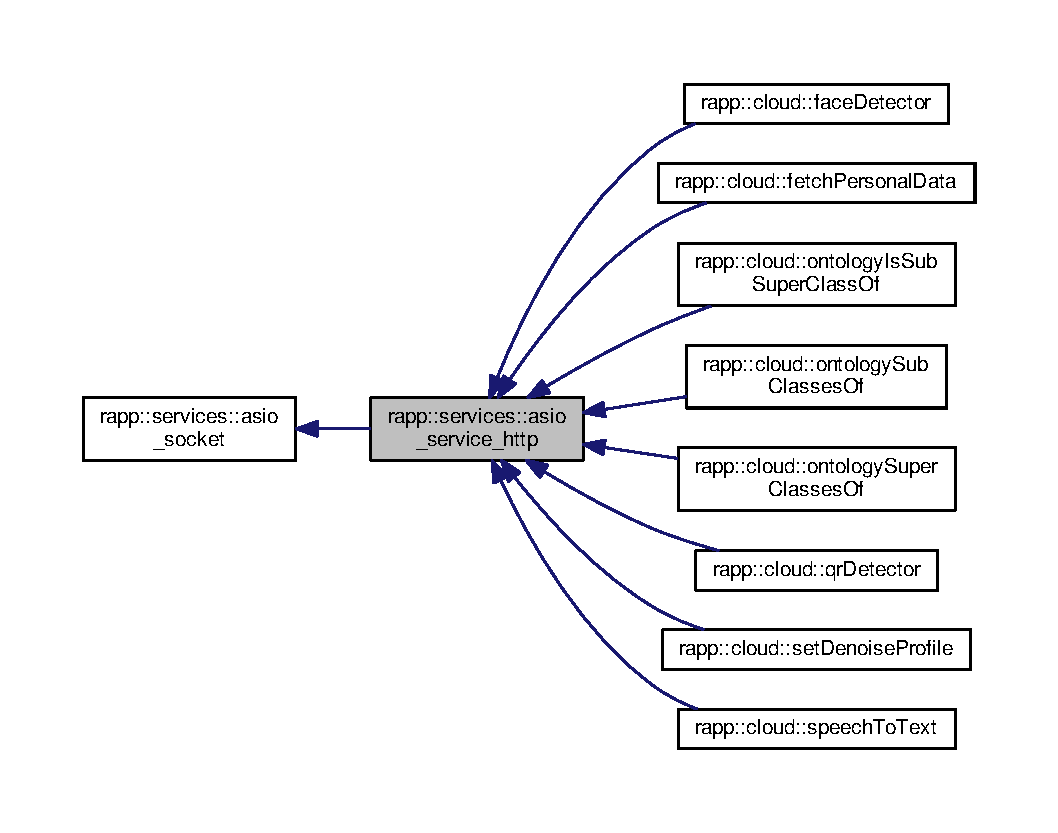
\includegraphics[width=350pt]{classrapp_1_1services_1_1asio__service__http__inherit__graph}
\end{center}
\end{figure}


Collaboration diagram for rapp\-:\-:services\-:\-:asio\-\_\-service\-\_\-http\-:
\nopagebreak
\begin{figure}[H]
\begin{center}
\leavevmode
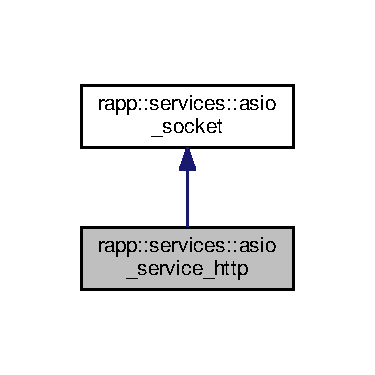
\includegraphics[width=180pt]{classrapp_1_1services_1_1asio__service__http__coll__graph}
\end{center}
\end{figure}
\subsection*{Public Member Functions}
\begin{DoxyCompactItemize}
\item 
void \hyperlink{classrapp_1_1services_1_1asio__service__http_ad95e973eef8650c5bbc8b90a95feac76}{Schedule} (boost\-::asio\-::ip\-::tcp\-::resolver\-::query \&query, boost\-::asio\-::ip\-::tcp\-::resolver \&resolver, boost\-::asio\-::io\-\_\-service \&io\-\_\-service)
\end{DoxyCompactItemize}
\subsection*{Protected Member Functions}
\begin{DoxyCompactItemize}
\item 
\hyperlink{classrapp_1_1services_1_1asio__service__http_a3ee5112e8a2d1f93e1a29e1ae97e0945}{asio\-\_\-service\-\_\-http} ()=default
\begin{DoxyCompactList}\small\item\em Hidden empty constructor is meant to be used only by inheriting classes. \end{DoxyCompactList}\item 
void \hyperlink{classrapp_1_1services_1_1asio__service__http_a3a8aeeda896612a34fbf519b5688aaa7}{error\-\_\-handler} (const boost\-::system\-::error\-\_\-code \&error)
\begin{DoxyCompactList}\small\item\em Handle an Error. \end{DoxyCompactList}\item 
void \hyperlink{classrapp_1_1services_1_1asio__service__http_a3a168f20797b06f722ebed12ad526e9b}{handle\-\_\-connect} (const boost\-::system\-::error\-\_\-code \&err, boost\-::asio\-::ip\-::tcp\-::resolver\-::iterator endpoint\-\_\-iterator)
\item 
void \hyperlink{classrapp_1_1services_1_1asio__service__http_ad8cdddec917928c476ce1f05205b6254}{handle\-\_\-read\-\_\-content} (const boost\-::system\-::error\-\_\-code \&err)
\begin{DoxyCompactList}\small\item\em Callback for Handling Actual Data Contents. \end{DoxyCompactList}\item 
void \hyperlink{classrapp_1_1services_1_1asio__service__http_a868568846ed87d1b551ce3e489e83754}{handle\-\_\-read\-\_\-headers} (const boost\-::system\-::error\-\_\-code \&err)
\begin{DoxyCompactList}\small\item\em Callback for Handling Headers. \end{DoxyCompactList}\item 
void \hyperlink{classrapp_1_1services_1_1asio__service__http_ad226cd37d18a2a67aad14e4d33f36ad1}{handle\-\_\-read\-\_\-status\-\_\-line} (const boost\-::system\-::error\-\_\-code \&err)
\begin{DoxyCompactList}\small\item\em Callback for handling H\-T\-T\-P Header Response Data. \end{DoxyCompactList}\item 
void \hyperlink{classrapp_1_1services_1_1asio__service__http_a046d89a8bca90438e131aae591cdc593}{handle\-\_\-resolve} (const boost\-::system\-::error\-\_\-code \&err, boost\-::asio\-::ip\-::tcp\-::resolver\-::iterator endpoint\-\_\-iterator)
\begin{DoxyCompactList}\small\item\em Callback for Handling Address Resolution. \end{DoxyCompactList}\item 
void \hyperlink{classrapp_1_1services_1_1asio__service__http_a2f1e6bf1f287798b48c671ce9596948a}{handle\-\_\-write\-\_\-request} (const boost\-::system\-::error\-\_\-code \&err)
\begin{DoxyCompactList}\small\item\em Callback for handling request and waiting for response. \end{DoxyCompactList}\item 
void \hyperlink{classrapp_1_1services_1_1asio__service__http_abcf7c541c4bf587da464ef24fa446743}{invalid\-\_\-request} (const std\-::string message)
\begin{DoxyCompactList}\small\item\em Handle Invalid Query -\/ e.\-g.\-: response which states our query was invalid. \end{DoxyCompactList}\item 
std\-::string \hyperlink{classrapp_1_1services_1_1asio__service__http_a11439cf4cd0a2a943bce9e91018fe8e0}{random\-Boundary} () const 
\begin{DoxyCompactList}\small\item\em Create a random boundary for the multipart/form in H\-T\-T\-P. \end{DoxyCompactList}\end{DoxyCompactItemize}
\subsection*{Protected Attributes}
\begin{DoxyCompactItemize}
\item 
std\-::function$<$ void(std\-::string)$>$ \hyperlink{classrapp_1_1services_1_1asio__service__http_a7ad60e0e171d8953da18e0c4e3974a80}{callback\-\_\-}
\begin{DoxyCompactList}\small\item\em Callback Handler -\/ use with std\-::bind or boost variant. \end{DoxyCompactList}\item 
std\-::string \hyperlink{classrapp_1_1services_1_1asio__service__http_ad2fbb8fb1f17c8ad6022ecbf13bc769c}{header\-\_\-}
\begin{DoxyCompactList}\small\item\em Header that will be used. \end{DoxyCompactList}\item 
std\-::string \hyperlink{classrapp_1_1services_1_1asio__service__http_a08e5b2c94340f528191e7840656be121}{post\-\_\-}
\begin{DoxyCompactList}\small\item\em Actual post Data. \end{DoxyCompactList}\item 
boost\-::asio\-::streambuf \hyperlink{classrapp_1_1services_1_1asio__service__http_a003a0577751d30d2370bff9a20d46746}{request\-\_\-}
\begin{DoxyCompactList}\small\item\em Request Container. \end{DoxyCompactList}\item 
boost\-::asio\-::streambuf \hyperlink{classrapp_1_1services_1_1asio__service__http_a5b1a5c59d1407fec9f0ccbe372bdac3a}{response\-\_\-}
\begin{DoxyCompactList}\small\item\em Response Container. \end{DoxyCompactList}\item 
std\-::unique\-\_\-ptr\\*
$<$ boost\-::asio\-::ip\-::tcp\-::socket $>$ \hyperlink{classrapp_1_1services_1_1asio__service__http_ad3411584026eb6c31ac78943266e7858}{socket\-\_\-}
\begin{DoxyCompactList}\small\item\em Actual Socket. \end{DoxyCompactList}\end{DoxyCompactItemize}


\subsection{Detailed Description}
base class for asynchronous http websockets used for connecting to cloud services 

\begin{DoxyVersion}{Version}
6 
\end{DoxyVersion}
\begin{DoxyDate}{Date}
26-\/\-April-\/2015 
\end{DoxyDate}
\begin{DoxyAuthor}{Author}
Alex Gkiokas \href{mailto:a.gkiokas@ortelio.co.uk}{\tt a.\-gkiokas@ortelio.\-co.\-uk}
\end{DoxyAuthor}
\begin{DoxySeeAlso}{See Also}
\href{http://www.jmarshall.com/easy/http/#postmethod}{\tt http\-://www.\-jmarshall.\-com/easy/http/\#postmethod} for H\-T\-T\-P Protocol details 
\end{DoxySeeAlso}
\begin{DoxyWarning}{Warning}
this class does not support S\-S\-L/\-T\-L\-S sockets 
\end{DoxyWarning}


Definition at line 18 of file asio\-\_\-service\-\_\-http.\-hpp.



\subsection{Constructor \& Destructor Documentation}
\hypertarget{classrapp_1_1services_1_1asio__service__http_a3ee5112e8a2d1f93e1a29e1ae97e0945}{\index{rapp\-::services\-::asio\-\_\-service\-\_\-http@{rapp\-::services\-::asio\-\_\-service\-\_\-http}!asio\-\_\-service\-\_\-http@{asio\-\_\-service\-\_\-http}}
\index{asio\-\_\-service\-\_\-http@{asio\-\_\-service\-\_\-http}!rapp::services::asio_service_http@{rapp\-::services\-::asio\-\_\-service\-\_\-http}}
\subsubsection[{asio\-\_\-service\-\_\-http}]{\setlength{\rightskip}{0pt plus 5cm}rapp\-::services\-::asio\-\_\-service\-\_\-http\-::asio\-\_\-service\-\_\-http (
\begin{DoxyParamCaption}
{}
\end{DoxyParamCaption}
)\hspace{0.3cm}{\ttfamily [protected]}, {\ttfamily [default]}}}\label{classrapp_1_1services_1_1asio__service__http_a3ee5112e8a2d1f93e1a29e1ae97e0945}


Hidden empty constructor is meant to be used only by inheriting classes. 



\subsection{Member Function Documentation}
\hypertarget{classrapp_1_1services_1_1asio__service__http_a3a8aeeda896612a34fbf519b5688aaa7}{\index{rapp\-::services\-::asio\-\_\-service\-\_\-http@{rapp\-::services\-::asio\-\_\-service\-\_\-http}!error\-\_\-handler@{error\-\_\-handler}}
\index{error\-\_\-handler@{error\-\_\-handler}!rapp::services::asio_service_http@{rapp\-::services\-::asio\-\_\-service\-\_\-http}}
\subsubsection[{error\-\_\-handler}]{\setlength{\rightskip}{0pt plus 5cm}void rapp\-::services\-::asio\-\_\-service\-\_\-http\-::error\-\_\-handler (
\begin{DoxyParamCaption}
\item[{const boost\-::system\-::error\-\_\-code \&}]{error}
\end{DoxyParamCaption}
)\hspace{0.3cm}{\ttfamily [protected]}}}\label{classrapp_1_1services_1_1asio__service__http_a3a8aeeda896612a34fbf519b5688aaa7}


Handle an Error. 


\begin{DoxyParams}{Parameters}
{\em error} & is the raised error from the client \\
\hline
\end{DoxyParams}


Definition at line 53 of file asio\-\_\-service\-\_\-http.\-hpp.

\hypertarget{classrapp_1_1services_1_1asio__service__http_a3a168f20797b06f722ebed12ad526e9b}{\index{rapp\-::services\-::asio\-\_\-service\-\_\-http@{rapp\-::services\-::asio\-\_\-service\-\_\-http}!handle\-\_\-connect@{handle\-\_\-connect}}
\index{handle\-\_\-connect@{handle\-\_\-connect}!rapp::services::asio_service_http@{rapp\-::services\-::asio\-\_\-service\-\_\-http}}
\subsubsection[{handle\-\_\-connect}]{\setlength{\rightskip}{0pt plus 5cm}void rapp\-::services\-::asio\-\_\-service\-\_\-http\-::handle\-\_\-connect (
\begin{DoxyParamCaption}
\item[{const boost\-::system\-::error\-\_\-code \&}]{err, }
\item[{boost\-::asio\-::ip\-::tcp\-::resolver\-::iterator}]{endpoint\-\_\-iterator}
\end{DoxyParamCaption}
)\hspace{0.3cm}{\ttfamily [protected]}}}\label{classrapp_1_1services_1_1asio__service__http_a3a168f20797b06f722ebed12ad526e9b}
Callback for Handling Connection Events 
\begin{DoxyParams}{Parameters}
{\em err} & is a possible error \\
\hline
{\em endpoint\-\_\-iterator} & is boosts' hostname address handler \\
\hline
\end{DoxyParams}


Definition at line 93 of file asio\-\_\-service\-\_\-http.\-hpp.

\hypertarget{classrapp_1_1services_1_1asio__service__http_ad8cdddec917928c476ce1f05205b6254}{\index{rapp\-::services\-::asio\-\_\-service\-\_\-http@{rapp\-::services\-::asio\-\_\-service\-\_\-http}!handle\-\_\-read\-\_\-content@{handle\-\_\-read\-\_\-content}}
\index{handle\-\_\-read\-\_\-content@{handle\-\_\-read\-\_\-content}!rapp::services::asio_service_http@{rapp\-::services\-::asio\-\_\-service\-\_\-http}}
\subsubsection[{handle\-\_\-read\-\_\-content}]{\setlength{\rightskip}{0pt plus 5cm}void rapp\-::services\-::asio\-\_\-service\-\_\-http\-::handle\-\_\-read\-\_\-content (
\begin{DoxyParamCaption}
\item[{const boost\-::system\-::error\-\_\-code \&}]{err}
\end{DoxyParamCaption}
)\hspace{0.3cm}{\ttfamily [protected]}}}\label{classrapp_1_1services_1_1asio__service__http_ad8cdddec917928c476ce1f05205b6254}


Callback for Handling Actual Data Contents. 


\begin{DoxyParams}{Parameters}
{\em err} & is a possible error message \\
\hline
\end{DoxyParams}


Definition at line 193 of file asio\-\_\-service\-\_\-http.\-hpp.

\hypertarget{classrapp_1_1services_1_1asio__service__http_a868568846ed87d1b551ce3e489e83754}{\index{rapp\-::services\-::asio\-\_\-service\-\_\-http@{rapp\-::services\-::asio\-\_\-service\-\_\-http}!handle\-\_\-read\-\_\-headers@{handle\-\_\-read\-\_\-headers}}
\index{handle\-\_\-read\-\_\-headers@{handle\-\_\-read\-\_\-headers}!rapp::services::asio_service_http@{rapp\-::services\-::asio\-\_\-service\-\_\-http}}
\subsubsection[{handle\-\_\-read\-\_\-headers}]{\setlength{\rightskip}{0pt plus 5cm}void rapp\-::services\-::asio\-\_\-service\-\_\-http\-::handle\-\_\-read\-\_\-headers (
\begin{DoxyParamCaption}
\item[{const boost\-::system\-::error\-\_\-code \&}]{err}
\end{DoxyParamCaption}
)\hspace{0.3cm}{\ttfamily [protected]}}}\label{classrapp_1_1services_1_1asio__service__http_a868568846ed87d1b551ce3e489e83754}


Callback for Handling Headers. 


\begin{DoxyParams}{Parameters}
{\em err} & is a possible error message \\
\hline
\end{DoxyParams}


Definition at line 176 of file asio\-\_\-service\-\_\-http.\-hpp.

\hypertarget{classrapp_1_1services_1_1asio__service__http_ad226cd37d18a2a67aad14e4d33f36ad1}{\index{rapp\-::services\-::asio\-\_\-service\-\_\-http@{rapp\-::services\-::asio\-\_\-service\-\_\-http}!handle\-\_\-read\-\_\-status\-\_\-line@{handle\-\_\-read\-\_\-status\-\_\-line}}
\index{handle\-\_\-read\-\_\-status\-\_\-line@{handle\-\_\-read\-\_\-status\-\_\-line}!rapp::services::asio_service_http@{rapp\-::services\-::asio\-\_\-service\-\_\-http}}
\subsubsection[{handle\-\_\-read\-\_\-status\-\_\-line}]{\setlength{\rightskip}{0pt plus 5cm}void rapp\-::services\-::asio\-\_\-service\-\_\-http\-::handle\-\_\-read\-\_\-status\-\_\-line (
\begin{DoxyParamCaption}
\item[{const boost\-::system\-::error\-\_\-code \&}]{err}
\end{DoxyParamCaption}
)\hspace{0.3cm}{\ttfamily [protected]}}}\label{classrapp_1_1services_1_1asio__service__http_ad226cd37d18a2a67aad14e4d33f36ad1}


Callback for handling H\-T\-T\-P Header Response Data. 


\begin{DoxyParams}{Parameters}
{\em err} & is a possible error message \\
\hline
\end{DoxyParams}


Definition at line 139 of file asio\-\_\-service\-\_\-http.\-hpp.

\hypertarget{classrapp_1_1services_1_1asio__service__http_a046d89a8bca90438e131aae591cdc593}{\index{rapp\-::services\-::asio\-\_\-service\-\_\-http@{rapp\-::services\-::asio\-\_\-service\-\_\-http}!handle\-\_\-resolve@{handle\-\_\-resolve}}
\index{handle\-\_\-resolve@{handle\-\_\-resolve}!rapp::services::asio_service_http@{rapp\-::services\-::asio\-\_\-service\-\_\-http}}
\subsubsection[{handle\-\_\-resolve}]{\setlength{\rightskip}{0pt plus 5cm}void rapp\-::services\-::asio\-\_\-service\-\_\-http\-::handle\-\_\-resolve (
\begin{DoxyParamCaption}
\item[{const boost\-::system\-::error\-\_\-code \&}]{err, }
\item[{boost\-::asio\-::ip\-::tcp\-::resolver\-::iterator}]{endpoint\-\_\-iterator}
\end{DoxyParamCaption}
)\hspace{0.3cm}{\ttfamily [protected]}}}\label{classrapp_1_1services_1_1asio__service__http_a046d89a8bca90438e131aae591cdc593}


Callback for Handling Address Resolution. 


\begin{DoxyParams}{Parameters}
{\em err} & is a possible error \\
\hline
{\em endpoint\-\_\-iterator} & is boost's hostname address handler \\
\hline
\end{DoxyParams}


Definition at line 69 of file asio\-\_\-service\-\_\-http.\-hpp.

\hypertarget{classrapp_1_1services_1_1asio__service__http_a2f1e6bf1f287798b48c671ce9596948a}{\index{rapp\-::services\-::asio\-\_\-service\-\_\-http@{rapp\-::services\-::asio\-\_\-service\-\_\-http}!handle\-\_\-write\-\_\-request@{handle\-\_\-write\-\_\-request}}
\index{handle\-\_\-write\-\_\-request@{handle\-\_\-write\-\_\-request}!rapp::services::asio_service_http@{rapp\-::services\-::asio\-\_\-service\-\_\-http}}
\subsubsection[{handle\-\_\-write\-\_\-request}]{\setlength{\rightskip}{0pt plus 5cm}void rapp\-::services\-::asio\-\_\-service\-\_\-http\-::handle\-\_\-write\-\_\-request (
\begin{DoxyParamCaption}
\item[{const boost\-::system\-::error\-\_\-code \&}]{err}
\end{DoxyParamCaption}
)\hspace{0.3cm}{\ttfamily [protected]}}}\label{classrapp_1_1services_1_1asio__service__http_a2f1e6bf1f287798b48c671ce9596948a}


Callback for handling request and waiting for response. 


\begin{DoxyParams}{Parameters}
{\em err} & is a possible error \\
\hline
\end{DoxyParams}


Definition at line 121 of file asio\-\_\-service\-\_\-http.\-hpp.

\hypertarget{classrapp_1_1services_1_1asio__service__http_abcf7c541c4bf587da464ef24fa446743}{\index{rapp\-::services\-::asio\-\_\-service\-\_\-http@{rapp\-::services\-::asio\-\_\-service\-\_\-http}!invalid\-\_\-request@{invalid\-\_\-request}}
\index{invalid\-\_\-request@{invalid\-\_\-request}!rapp::services::asio_service_http@{rapp\-::services\-::asio\-\_\-service\-\_\-http}}
\subsubsection[{invalid\-\_\-request}]{\setlength{\rightskip}{0pt plus 5cm}void rapp\-::services\-::asio\-\_\-service\-\_\-http\-::invalid\-\_\-request (
\begin{DoxyParamCaption}
\item[{const std\-::string}]{message}
\end{DoxyParamCaption}
)\hspace{0.3cm}{\ttfamily [protected]}}}\label{classrapp_1_1services_1_1asio__service__http_abcf7c541c4bf587da464ef24fa446743}


Handle Invalid Query -\/ e.\-g.\-: response which states our query was invalid. 


\begin{DoxyParams}{Parameters}
{\em message} & is the message received from the service \\
\hline
\end{DoxyParams}


Definition at line 59 of file asio\-\_\-service\-\_\-http.\-hpp.

\hypertarget{classrapp_1_1services_1_1asio__service__http_a11439cf4cd0a2a943bce9e91018fe8e0}{\index{rapp\-::services\-::asio\-\_\-service\-\_\-http@{rapp\-::services\-::asio\-\_\-service\-\_\-http}!random\-Boundary@{random\-Boundary}}
\index{random\-Boundary@{random\-Boundary}!rapp::services::asio_service_http@{rapp\-::services\-::asio\-\_\-service\-\_\-http}}
\subsubsection[{random\-Boundary}]{\setlength{\rightskip}{0pt plus 5cm}std\-::string rapp\-::services\-::asio\-\_\-service\-\_\-http\-::random\-Boundary (
\begin{DoxyParamCaption}
{}
\end{DoxyParamCaption}
) const\hspace{0.3cm}{\ttfamily [protected]}}}\label{classrapp_1_1services_1_1asio__service__http_a11439cf4cd0a2a943bce9e91018fe8e0}


Create a random boundary for the multipart/form in H\-T\-T\-P. 



Definition at line 226 of file asio\-\_\-service\-\_\-http.\-hpp.

\hypertarget{classrapp_1_1services_1_1asio__service__http_ad95e973eef8650c5bbc8b90a95feac76}{\index{rapp\-::services\-::asio\-\_\-service\-\_\-http@{rapp\-::services\-::asio\-\_\-service\-\_\-http}!Schedule@{Schedule}}
\index{Schedule@{Schedule}!rapp::services::asio_service_http@{rapp\-::services\-::asio\-\_\-service\-\_\-http}}
\subsubsection[{Schedule}]{\setlength{\rightskip}{0pt plus 5cm}void rapp\-::services\-::asio\-\_\-service\-\_\-http\-::\-Schedule (
\begin{DoxyParamCaption}
\item[{boost\-::asio\-::ip\-::tcp\-::resolver\-::query \&}]{query, }
\item[{boost\-::asio\-::ip\-::tcp\-::resolver \&}]{resolver, }
\item[{boost\-::asio\-::io\-\_\-service \&}]{io\-\_\-service}
\end{DoxyParamCaption}
)\hspace{0.3cm}{\ttfamily [virtual]}}}\label{classrapp_1_1services_1_1asio__service__http_ad95e973eef8650c5bbc8b90a95feac76}
Schedule this client as a job for execution using 
\begin{DoxyParams}{Parameters}
{\em query} & defines the actual U\-R\-L/\-U\-R\-I \\
\hline
{\em resolver} & is the U\-R\-L/\-U\-R\-I resolver reference \\
\hline
{\em io\-\_\-service} & is the service queue on which this job will be scheduled to run \\
\hline
\end{DoxyParams}


Implements \hyperlink{classrapp_1_1services_1_1asio__socket_a1241f0694fea6c2f13c361ddef13360b}{rapp\-::services\-::asio\-\_\-socket}.



Definition at line 28 of file asio\-\_\-service\-\_\-http.\-hpp.



\subsection{Member Data Documentation}
\hypertarget{classrapp_1_1services_1_1asio__service__http_a7ad60e0e171d8953da18e0c4e3974a80}{\index{rapp\-::services\-::asio\-\_\-service\-\_\-http@{rapp\-::services\-::asio\-\_\-service\-\_\-http}!callback\-\_\-@{callback\-\_\-}}
\index{callback\-\_\-@{callback\-\_\-}!rapp::services::asio_service_http@{rapp\-::services\-::asio\-\_\-service\-\_\-http}}
\subsubsection[{callback\-\_\-}]{\setlength{\rightskip}{0pt plus 5cm}std\-::function$<$void( std\-::string )$>$ rapp\-::services\-::asio\-\_\-service\-\_\-http\-::callback\-\_\-\hspace{0.3cm}{\ttfamily [protected]}}}\label{classrapp_1_1services_1_1asio__service__http_a7ad60e0e171d8953da18e0c4e3974a80}


Callback Handler -\/ use with std\-::bind or boost variant. 



Definition at line 251 of file asio\-\_\-service\-\_\-http.\-hpp.

\hypertarget{classrapp_1_1services_1_1asio__service__http_ad2fbb8fb1f17c8ad6022ecbf13bc769c}{\index{rapp\-::services\-::asio\-\_\-service\-\_\-http@{rapp\-::services\-::asio\-\_\-service\-\_\-http}!header\-\_\-@{header\-\_\-}}
\index{header\-\_\-@{header\-\_\-}!rapp::services::asio_service_http@{rapp\-::services\-::asio\-\_\-service\-\_\-http}}
\subsubsection[{header\-\_\-}]{\setlength{\rightskip}{0pt plus 5cm}std\-::string rapp\-::services\-::asio\-\_\-service\-\_\-http\-::header\-\_\-\hspace{0.3cm}{\ttfamily [protected]}}}\label{classrapp_1_1services_1_1asio__service__http_ad2fbb8fb1f17c8ad6022ecbf13bc769c}


Header that will be used. 



Definition at line 245 of file asio\-\_\-service\-\_\-http.\-hpp.

\hypertarget{classrapp_1_1services_1_1asio__service__http_a08e5b2c94340f528191e7840656be121}{\index{rapp\-::services\-::asio\-\_\-service\-\_\-http@{rapp\-::services\-::asio\-\_\-service\-\_\-http}!post\-\_\-@{post\-\_\-}}
\index{post\-\_\-@{post\-\_\-}!rapp::services::asio_service_http@{rapp\-::services\-::asio\-\_\-service\-\_\-http}}
\subsubsection[{post\-\_\-}]{\setlength{\rightskip}{0pt plus 5cm}std\-::string rapp\-::services\-::asio\-\_\-service\-\_\-http\-::post\-\_\-\hspace{0.3cm}{\ttfamily [protected]}}}\label{classrapp_1_1services_1_1asio__service__http_a08e5b2c94340f528191e7840656be121}


Actual post Data. 



Definition at line 248 of file asio\-\_\-service\-\_\-http.\-hpp.

\hypertarget{classrapp_1_1services_1_1asio__service__http_a003a0577751d30d2370bff9a20d46746}{\index{rapp\-::services\-::asio\-\_\-service\-\_\-http@{rapp\-::services\-::asio\-\_\-service\-\_\-http}!request\-\_\-@{request\-\_\-}}
\index{request\-\_\-@{request\-\_\-}!rapp::services::asio_service_http@{rapp\-::services\-::asio\-\_\-service\-\_\-http}}
\subsubsection[{request\-\_\-}]{\setlength{\rightskip}{0pt plus 5cm}boost\-::asio\-::streambuf rapp\-::services\-::asio\-\_\-service\-\_\-http\-::request\-\_\-\hspace{0.3cm}{\ttfamily [protected]}}}\label{classrapp_1_1services_1_1asio__service__http_a003a0577751d30d2370bff9a20d46746}


Request Container. 



Definition at line 257 of file asio\-\_\-service\-\_\-http.\-hpp.

\hypertarget{classrapp_1_1services_1_1asio__service__http_a5b1a5c59d1407fec9f0ccbe372bdac3a}{\index{rapp\-::services\-::asio\-\_\-service\-\_\-http@{rapp\-::services\-::asio\-\_\-service\-\_\-http}!response\-\_\-@{response\-\_\-}}
\index{response\-\_\-@{response\-\_\-}!rapp::services::asio_service_http@{rapp\-::services\-::asio\-\_\-service\-\_\-http}}
\subsubsection[{response\-\_\-}]{\setlength{\rightskip}{0pt plus 5cm}boost\-::asio\-::streambuf rapp\-::services\-::asio\-\_\-service\-\_\-http\-::response\-\_\-\hspace{0.3cm}{\ttfamily [protected]}}}\label{classrapp_1_1services_1_1asio__service__http_a5b1a5c59d1407fec9f0ccbe372bdac3a}


Response Container. 



Definition at line 260 of file asio\-\_\-service\-\_\-http.\-hpp.

\hypertarget{classrapp_1_1services_1_1asio__service__http_ad3411584026eb6c31ac78943266e7858}{\index{rapp\-::services\-::asio\-\_\-service\-\_\-http@{rapp\-::services\-::asio\-\_\-service\-\_\-http}!socket\-\_\-@{socket\-\_\-}}
\index{socket\-\_\-@{socket\-\_\-}!rapp::services::asio_service_http@{rapp\-::services\-::asio\-\_\-service\-\_\-http}}
\subsubsection[{socket\-\_\-}]{\setlength{\rightskip}{0pt plus 5cm}std\-::unique\-\_\-ptr$<$boost\-::asio\-::ip\-::tcp\-::socket$>$ rapp\-::services\-::asio\-\_\-service\-\_\-http\-::socket\-\_\-\hspace{0.3cm}{\ttfamily [protected]}}}\label{classrapp_1_1services_1_1asio__service__http_ad3411584026eb6c31ac78943266e7858}


Actual Socket. 



Definition at line 254 of file asio\-\_\-service\-\_\-http.\-hpp.



The documentation for this class was generated from the following file\-:\begin{DoxyCompactItemize}
\item 
/home/travis/rapp\-\_\-temp/rapp-\/api/cpp/includes/service/asio\-\_\-service\-\_\-http/\hyperlink{asio__service__http_8hpp}{asio\-\_\-service\-\_\-http.\-hpp}\end{DoxyCompactItemize}

\hypertarget{classrapp_1_1services_1_1asio__service__raw}{\section{rapp\-:\-:services\-:\-:asio\-\_\-service\-\_\-raw Class Reference}
\label{classrapp_1_1services_1_1asio__service__raw}\index{rapp\-::services\-::asio\-\_\-service\-\_\-raw@{rapp\-::services\-::asio\-\_\-service\-\_\-raw}}
}


base class for asynchronous sockets used for connecting to cloud services  




{\ttfamily \#include $<$asio\-\_\-service\-\_\-raw.\-hpp$>$}



Inheritance diagram for rapp\-:\-:services\-:\-:asio\-\_\-service\-\_\-raw\-:
\nopagebreak
\begin{figure}[H]
\begin{center}
\leavevmode
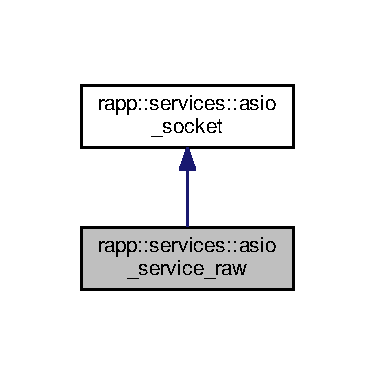
\includegraphics[width=180pt]{classrapp_1_1services_1_1asio__service__raw__inherit__graph}
\end{center}
\end{figure}


Collaboration diagram for rapp\-:\-:services\-:\-:asio\-\_\-service\-\_\-raw\-:
\nopagebreak
\begin{figure}[H]
\begin{center}
\leavevmode
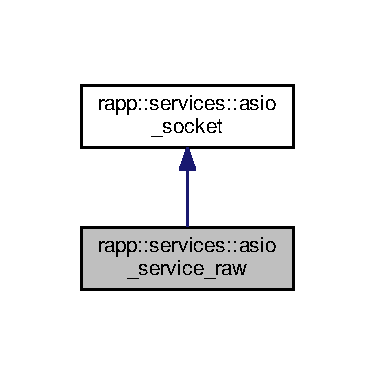
\includegraphics[width=180pt]{classrapp_1_1services_1_1asio__service__raw__coll__graph}
\end{center}
\end{figure}
\subsection*{Public Member Functions}
\begin{DoxyCompactItemize}
\item 
\hyperlink{classrapp_1_1services_1_1asio__service__raw_a9f6dc2b1905cd926ef7cef5c2616aefc}{asio\-\_\-service\-\_\-raw} (const std\-::vector$<$ \hyperlink{namespacerapp_1_1types_a1dbc9dc2ab4507d8fb58ac3a204d307b}{rapp\-::types\-::byte} $>$ \&bytearray)
\begin{DoxyCompactList}\small\item\em Construct an Asynchronous Socket Client without H\-T\-T\-P stuff, only X\-M\-L delimiters. \end{DoxyCompactList}\item 
\hyperlink{classrapp_1_1services_1_1asio__service__raw_aafd14d12bd6cb0000380263e454b3f26}{asio\-\_\-service\-\_\-raw} (const std\-::vector$<$ \hyperlink{namespacerapp_1_1types_a1dbc9dc2ab4507d8fb58ac3a204d307b}{rapp\-::types\-::byte} $>$ \&bytearray, std\-::function$<$ void(boost\-::asio\-::streambuf \&)$>$ callback)
\begin{DoxyCompactList}\small\item\em Construct an Asynchronous Socket Client without H\-T\-T\-P stuff, only X\-M\-L delimiters. \end{DoxyCompactList}\item 
void \hyperlink{classrapp_1_1services_1_1asio__service__raw_a11078ec812461792f81bca299db468ce}{Schedule} (boost\-::asio\-::ip\-::tcp\-::resolver\-::query \&query, boost\-::asio\-::ip\-::tcp\-::resolver \&resolver, boost\-::asio\-::io\-\_\-service \&io\-\_\-service)
\end{DoxyCompactItemize}
\subsection*{Protected Member Functions}
\begin{DoxyCompactItemize}
\item 
virtual void \hyperlink{classrapp_1_1services_1_1asio__service__raw_a96fe160b9973c6316df16d0ec2939104}{error\-\_\-handler} (const boost\-::system\-::error\-\_\-code \&error)
\item 
void \hyperlink{classrapp_1_1services_1_1asio__service__raw_a8be2c6ac66884d8d3f3779c2c70651c1}{handle\-\_\-connect} (const boost\-::system\-::error\-\_\-code \&err, boost\-::asio\-::ip\-::tcp\-::resolver\-::iterator endpoint\-\_\-iterator)
\item 
void \hyperlink{classrapp_1_1services_1_1asio__service__raw_a053752763ff279a21718da71b317aa6f}{handle\-\_\-read\-\_\-response} (const boost\-::system\-::error\-\_\-code \&err)
\item 
virtual void \hyperlink{classrapp_1_1services_1_1asio__service__raw_a16180f18d857607b862e5a63793e8faf}{handle\-\_\-reply} ()
\item 
void \hyperlink{classrapp_1_1services_1_1asio__service__raw_afe3816c68db5367968f237e863b5ecb4}{handle\-\_\-resolve} (const boost\-::system\-::error\-\_\-code \&err, boost\-::asio\-::ip\-::tcp\-::resolver\-::iterator endpoint\-\_\-iterator)
\item 
void \hyperlink{classrapp_1_1services_1_1asio__service__raw_a44819785fc02d1583d2325ea4ddfd93d}{handle\-\_\-write\-\_\-request} (const boost\-::system\-::error\-\_\-code \&err)
\end{DoxyCompactItemize}
\subsection*{Protected Attributes}
\begin{DoxyCompactItemize}
\item 
std\-::vector$<$ \hyperlink{namespacerapp_1_1types_a1dbc9dc2ab4507d8fb58ac3a204d307b}{rapp\-::types\-::byte} $>$ \hyperlink{classrapp_1_1services_1_1asio__service__raw_a79ed79443645b99131fb7d1b215e14bc}{bytes\-\_\-}
\begin{DoxyCompactList}\small\item\em Actual bytestream that will be sent over the socket -\/. \end{DoxyCompactList}\item 
std\-::function$<$ void(boost\-::asio\-::streambuf \&)$>$ \hyperlink{classrapp_1_1services_1_1asio__service__raw_a045f535c43a9fa18df911b7d73332358}{callback\-\_\-}
\begin{DoxyCompactList}\small\item\em Optional Callback Handler. \end{DoxyCompactList}\item 
bool \hyperlink{classrapp_1_1services_1_1asio__service__raw_a24f0666266885acbe7a2fa260f7a5383}{complete\-\_\-} = false
\begin{DoxyCompactList}\small\item\em Operation complete? \end{DoxyCompactList}\item 
boost\-::asio\-::streambuf \hyperlink{classrapp_1_1services_1_1asio__service__raw_a6d53e73589def6049fda150fab228df8}{request\-\_\-}
\begin{DoxyCompactList}\small\item\em Request buffer stream. \end{DoxyCompactList}\item 
boost\-::asio\-::streambuf \hyperlink{classrapp_1_1services_1_1asio__service__raw_a94d17ec39af125c8cfaef0db42ae1aac}{response\-\_\-}
\begin{DoxyCompactList}\small\item\em Response buffer stream. \end{DoxyCompactList}\item 
std\-::unique\-\_\-ptr\\*
$<$ boost\-::asio\-::ip\-::tcp\-::socket $>$ \hyperlink{classrapp_1_1services_1_1asio__service__raw_a070f217b7642bd28f122bd3fb29e9540}{socket\-\_\-}
\begin{DoxyCompactList}\small\item\em Actual Socket. \end{DoxyCompactList}\end{DoxyCompactItemize}


\subsection{Detailed Description}
base class for asynchronous sockets used for connecting to cloud services 

\begin{DoxyVersion}{Version}
2 
\end{DoxyVersion}
\begin{DoxyDate}{Date}
6-\/\-February-\/2015 
\end{DoxyDate}
\begin{DoxyAuthor}{Author}
Alex Gkiokas \href{mailto:a.gkiokas@ortelio.co.uk}{\tt a.\-gkiokas@ortelio.\-co.\-uk} 
\end{DoxyAuthor}
\begin{DoxyWarning}{Warning}
this class does not support S\-S\-L/\-T\-L\-S sockets
\end{DoxyWarning}
W\-A\-R\-N\-I\-N\-G R\-E\-S\-T\-R\-U\-C\-T\-U\-R\-E A\-S H\-E\-A\-D\-E\-R O\-N\-L\-Y !!!! F\-A\-C\-I\-L\-I\-A\-T\-E T\-H\-E U\-S\-A\-G\-E O\-F S\-T\-R\-E\-A\-M\-I\-N\-G B\-U\-F\-F\-E\-R\-S F\-R\-O\-M C\-L\-I\-E\-N\-T T\-O S\-E\-R\-V\-E\-R A\-S T\-H\-I\-S I\-S T\-H\-E O\-N\-L\-Y T\-H\-I\-N\-G W\-E W\-I\-L\-L U\-S\-E T\-H\-I\-S C\-L\-A\-S\-S F\-O\-R !!!

W\-A\-R\-N\-I\-N\-G T\-H\-E virtual methods below are of no use -\/ see how \hyperlink{classrapp_1_1services_1_1asio__service__http}{asio\-\_\-service\-\_\-http} has been reworked and do the same here 

Definition at line 19 of file asio\-\_\-service\-\_\-raw.\-hpp.



\subsection{Constructor \& Destructor Documentation}
\hypertarget{classrapp_1_1services_1_1asio__service__raw_a9f6dc2b1905cd926ef7cef5c2616aefc}{\index{rapp\-::services\-::asio\-\_\-service\-\_\-raw@{rapp\-::services\-::asio\-\_\-service\-\_\-raw}!asio\-\_\-service\-\_\-raw@{asio\-\_\-service\-\_\-raw}}
\index{asio\-\_\-service\-\_\-raw@{asio\-\_\-service\-\_\-raw}!rapp::services::asio_service_raw@{rapp\-::services\-::asio\-\_\-service\-\_\-raw}}
\subsubsection[{asio\-\_\-service\-\_\-raw}]{\setlength{\rightskip}{0pt plus 5cm}rapp\-::services\-::asio\-\_\-service\-\_\-raw\-::asio\-\_\-service\-\_\-raw (
\begin{DoxyParamCaption}
\item[{const std\-::vector$<$ {\bf rapp\-::types\-::byte} $>$ \&}]{bytearray}
\end{DoxyParamCaption}
)}}\label{classrapp_1_1services_1_1asio__service__raw_a9f6dc2b1905cd926ef7cef5c2616aefc}


Construct an Asynchronous Socket Client without H\-T\-T\-P stuff, only X\-M\-L delimiters. 


\begin{DoxyParams}{Parameters}
{\em bytearray} & is a vector which contains raw byte (char) values \\
\hline
\end{DoxyParams}


Definition at line 7 of file asio\-\_\-service\-\_\-raw.\-cpp.

\hypertarget{classrapp_1_1services_1_1asio__service__raw_aafd14d12bd6cb0000380263e454b3f26}{\index{rapp\-::services\-::asio\-\_\-service\-\_\-raw@{rapp\-::services\-::asio\-\_\-service\-\_\-raw}!asio\-\_\-service\-\_\-raw@{asio\-\_\-service\-\_\-raw}}
\index{asio\-\_\-service\-\_\-raw@{asio\-\_\-service\-\_\-raw}!rapp::services::asio_service_raw@{rapp\-::services\-::asio\-\_\-service\-\_\-raw}}
\subsubsection[{asio\-\_\-service\-\_\-raw}]{\setlength{\rightskip}{0pt plus 5cm}rapp\-::services\-::asio\-\_\-service\-\_\-raw\-::asio\-\_\-service\-\_\-raw (
\begin{DoxyParamCaption}
\item[{const std\-::vector$<$ {\bf rapp\-::types\-::byte} $>$ \&}]{bytearray, }
\item[{std\-::function$<$ void(boost\-::asio\-::streambuf \&)$>$}]{callback}
\end{DoxyParamCaption}
)}}\label{classrapp_1_1services_1_1asio__service__raw_aafd14d12bd6cb0000380263e454b3f26}


Construct an Asynchronous Socket Client without H\-T\-T\-P stuff, only X\-M\-L delimiters. 


\begin{DoxyParams}{Parameters}
{\em bytearray} & is a vector which contains raw byte (char) values \\
\hline
{\em callback} & is a lamda or function pointer with the specific signature, that is invoked upon reply acquisition \\
\hline
\end{DoxyParams}


Definition at line 12 of file asio\-\_\-service\-\_\-raw.\-cpp.



\subsection{Member Function Documentation}
\hypertarget{classrapp_1_1services_1_1asio__service__raw_a96fe160b9973c6316df16d0ec2939104}{\index{rapp\-::services\-::asio\-\_\-service\-\_\-raw@{rapp\-::services\-::asio\-\_\-service\-\_\-raw}!error\-\_\-handler@{error\-\_\-handler}}
\index{error\-\_\-handler@{error\-\_\-handler}!rapp::services::asio_service_raw@{rapp\-::services\-::asio\-\_\-service\-\_\-raw}}
\subsubsection[{error\-\_\-handler}]{\setlength{\rightskip}{0pt plus 5cm}void rapp\-::services\-::asio\-\_\-service\-\_\-raw\-::error\-\_\-handler (
\begin{DoxyParamCaption}
\item[{const boost\-::system\-::error\-\_\-code \&}]{error}
\end{DoxyParamCaption}
)\hspace{0.3cm}{\ttfamily [protected]}, {\ttfamily [virtual]}}}\label{classrapp_1_1services_1_1asio__service__raw_a96fe160b9973c6316df16d0ec2939104}
Handle an Error 
\begin{DoxyParams}{Parameters}
{\em error} & is the raised error from the client \\
\hline
\end{DoxyParams}


Definition at line 52 of file asio\-\_\-service\-\_\-raw.\-cpp.

\hypertarget{classrapp_1_1services_1_1asio__service__raw_a8be2c6ac66884d8d3f3779c2c70651c1}{\index{rapp\-::services\-::asio\-\_\-service\-\_\-raw@{rapp\-::services\-::asio\-\_\-service\-\_\-raw}!handle\-\_\-connect@{handle\-\_\-connect}}
\index{handle\-\_\-connect@{handle\-\_\-connect}!rapp::services::asio_service_raw@{rapp\-::services\-::asio\-\_\-service\-\_\-raw}}
\subsubsection[{handle\-\_\-connect}]{\setlength{\rightskip}{0pt plus 5cm}void rapp\-::services\-::asio\-\_\-service\-\_\-raw\-::handle\-\_\-connect (
\begin{DoxyParamCaption}
\item[{const boost\-::system\-::error\-\_\-code \&}]{err, }
\item[{boost\-::asio\-::ip\-::tcp\-::resolver\-::iterator}]{endpoint\-\_\-iterator}
\end{DoxyParamCaption}
)\hspace{0.3cm}{\ttfamily [protected]}}}\label{classrapp_1_1services_1_1asio__service__raw_a8be2c6ac66884d8d3f3779c2c70651c1}
Callback for Handling Connection Events 
\begin{DoxyParams}{Parameters}
{\em err} & is a possible error \\
\hline
{\em endpoint\-\_\-iterator} & is boosts' hostname address handler \\
\hline
\end{DoxyParams}
W\-A\-R\-N\-I\-N\-G -\/ Make this time-\/out 

Definition at line 80 of file asio\-\_\-service\-\_\-raw.\-cpp.

\hypertarget{classrapp_1_1services_1_1asio__service__raw_a053752763ff279a21718da71b317aa6f}{\index{rapp\-::services\-::asio\-\_\-service\-\_\-raw@{rapp\-::services\-::asio\-\_\-service\-\_\-raw}!handle\-\_\-read\-\_\-response@{handle\-\_\-read\-\_\-response}}
\index{handle\-\_\-read\-\_\-response@{handle\-\_\-read\-\_\-response}!rapp::services::asio_service_raw@{rapp\-::services\-::asio\-\_\-service\-\_\-raw}}
\subsubsection[{handle\-\_\-read\-\_\-response}]{\setlength{\rightskip}{0pt plus 5cm}void rapp\-::services\-::asio\-\_\-service\-\_\-raw\-::handle\-\_\-read\-\_\-response (
\begin{DoxyParamCaption}
\item[{const boost\-::system\-::error\-\_\-code \&}]{err}
\end{DoxyParamCaption}
)\hspace{0.3cm}{\ttfamily [protected]}}}\label{classrapp_1_1services_1_1asio__service__raw_a053752763ff279a21718da71b317aa6f}
Callback for handling reading the reponse from the server 

Definition at line 134 of file asio\-\_\-service\-\_\-raw.\-cpp.

\hypertarget{classrapp_1_1services_1_1asio__service__raw_a16180f18d857607b862e5a63793e8faf}{\index{rapp\-::services\-::asio\-\_\-service\-\_\-raw@{rapp\-::services\-::asio\-\_\-service\-\_\-raw}!handle\-\_\-reply@{handle\-\_\-reply}}
\index{handle\-\_\-reply@{handle\-\_\-reply}!rapp::services::asio_service_raw@{rapp\-::services\-::asio\-\_\-service\-\_\-raw}}
\subsubsection[{handle\-\_\-reply}]{\setlength{\rightskip}{0pt plus 5cm}void rapp\-::services\-::asio\-\_\-service\-\_\-raw\-::handle\-\_\-reply (
\begin{DoxyParamCaption}
{}
\end{DoxyParamCaption}
)\hspace{0.3cm}{\ttfamily [protected]}, {\ttfamily [virtual]}}}\label{classrapp_1_1services_1_1asio__service__raw_a16180f18d857607b862e5a63793e8faf}
Handle the Reply \begin{DoxyNote}{Note}
you have to override this method if inheriting 
\end{DoxyNote}


Definition at line 45 of file asio\-\_\-service\-\_\-raw.\-cpp.

\hypertarget{classrapp_1_1services_1_1asio__service__raw_afe3816c68db5367968f237e863b5ecb4}{\index{rapp\-::services\-::asio\-\_\-service\-\_\-raw@{rapp\-::services\-::asio\-\_\-service\-\_\-raw}!handle\-\_\-resolve@{handle\-\_\-resolve}}
\index{handle\-\_\-resolve@{handle\-\_\-resolve}!rapp::services::asio_service_raw@{rapp\-::services\-::asio\-\_\-service\-\_\-raw}}
\subsubsection[{handle\-\_\-resolve}]{\setlength{\rightskip}{0pt plus 5cm}void rapp\-::services\-::asio\-\_\-service\-\_\-raw\-::handle\-\_\-resolve (
\begin{DoxyParamCaption}
\item[{const boost\-::system\-::error\-\_\-code \&}]{err, }
\item[{boost\-::asio\-::ip\-::tcp\-::resolver\-::iterator}]{endpoint\-\_\-iterator}
\end{DoxyParamCaption}
)\hspace{0.3cm}{\ttfamily [protected]}}}\label{classrapp_1_1services_1_1asio__service__raw_afe3816c68db5367968f237e863b5ecb4}
Callback for Handling Address Resolution 
\begin{DoxyParams}{Parameters}
{\em err} & is a possible error \\
\hline
{\em endpoint\-\_\-iterator} & is boost's hostname address handler \\
\hline
\end{DoxyParams}


Definition at line 57 of file asio\-\_\-service\-\_\-raw.\-cpp.

\hypertarget{classrapp_1_1services_1_1asio__service__raw_a44819785fc02d1583d2325ea4ddfd93d}{\index{rapp\-::services\-::asio\-\_\-service\-\_\-raw@{rapp\-::services\-::asio\-\_\-service\-\_\-raw}!handle\-\_\-write\-\_\-request@{handle\-\_\-write\-\_\-request}}
\index{handle\-\_\-write\-\_\-request@{handle\-\_\-write\-\_\-request}!rapp::services::asio_service_raw@{rapp\-::services\-::asio\-\_\-service\-\_\-raw}}
\subsubsection[{handle\-\_\-write\-\_\-request}]{\setlength{\rightskip}{0pt plus 5cm}void rapp\-::services\-::asio\-\_\-service\-\_\-raw\-::handle\-\_\-write\-\_\-request (
\begin{DoxyParamCaption}
\item[{const boost\-::system\-::error\-\_\-code \&}]{err}
\end{DoxyParamCaption}
)\hspace{0.3cm}{\ttfamily [protected]}}}\label{classrapp_1_1services_1_1asio__service__raw_a44819785fc02d1583d2325ea4ddfd93d}
Callback for handling sending request and waiting for a response 
\begin{DoxyParams}{Parameters}
{\em err} & is a possible error \\
\hline
\end{DoxyParams}
N\-O\-T\-E\-: Make this time-\/out, we don't want to wait forever for a reply! 

Definition at line 113 of file asio\-\_\-service\-\_\-raw.\-cpp.

\hypertarget{classrapp_1_1services_1_1asio__service__raw_a11078ec812461792f81bca299db468ce}{\index{rapp\-::services\-::asio\-\_\-service\-\_\-raw@{rapp\-::services\-::asio\-\_\-service\-\_\-raw}!Schedule@{Schedule}}
\index{Schedule@{Schedule}!rapp::services::asio_service_raw@{rapp\-::services\-::asio\-\_\-service\-\_\-raw}}
\subsubsection[{Schedule}]{\setlength{\rightskip}{0pt plus 5cm}void rapp\-::services\-::asio\-\_\-service\-\_\-raw\-::\-Schedule (
\begin{DoxyParamCaption}
\item[{boost\-::asio\-::ip\-::tcp\-::resolver\-::query \&}]{query, }
\item[{boost\-::asio\-::ip\-::tcp\-::resolver \&}]{resolver, }
\item[{boost\-::asio\-::io\-\_\-service \&}]{io\-\_\-service}
\end{DoxyParamCaption}
)\hspace{0.3cm}{\ttfamily [virtual]}}}\label{classrapp_1_1services_1_1asio__service__raw_a11078ec812461792f81bca299db468ce}
Schedule this client as a job for execution using 
\begin{DoxyParams}{Parameters}
{\em query} & defines the actual U\-R\-L/\-U\-R\-I \\
\hline
{\em resolver} & is the U\-R\-L/\-U\-R\-I resolver reference \\
\hline
{\em io\-\_\-service} & is the service queue on which this job will be scheduled to run \\
\hline
\end{DoxyParams}


Implements \hyperlink{classrapp_1_1services_1_1asio__socket_a1241f0694fea6c2f13c361ddef13360b}{rapp\-::services\-::asio\-\_\-socket}.



Definition at line 21 of file asio\-\_\-service\-\_\-raw.\-cpp.



\subsection{Member Data Documentation}
\hypertarget{classrapp_1_1services_1_1asio__service__raw_a79ed79443645b99131fb7d1b215e14bc}{\index{rapp\-::services\-::asio\-\_\-service\-\_\-raw@{rapp\-::services\-::asio\-\_\-service\-\_\-raw}!bytes\-\_\-@{bytes\-\_\-}}
\index{bytes\-\_\-@{bytes\-\_\-}!rapp::services::asio_service_raw@{rapp\-::services\-::asio\-\_\-service\-\_\-raw}}
\subsubsection[{bytes\-\_\-}]{\setlength{\rightskip}{0pt plus 5cm}std\-::vector$<${\bf rapp\-::types\-::byte}$>$ rapp\-::services\-::asio\-\_\-service\-\_\-raw\-::bytes\-\_\-\hspace{0.3cm}{\ttfamily [protected]}}}\label{classrapp_1_1services_1_1asio__service__raw_a79ed79443645b99131fb7d1b215e14bc}


Actual bytestream that will be sent over the socket -\/. 

\begin{DoxyNote}{Note}
\-: be careful not to consume it prematurely! 
\end{DoxyNote}


Definition at line 99 of file asio\-\_\-service\-\_\-raw.\-hpp.

\hypertarget{classrapp_1_1services_1_1asio__service__raw_a045f535c43a9fa18df911b7d73332358}{\index{rapp\-::services\-::asio\-\_\-service\-\_\-raw@{rapp\-::services\-::asio\-\_\-service\-\_\-raw}!callback\-\_\-@{callback\-\_\-}}
\index{callback\-\_\-@{callback\-\_\-}!rapp::services::asio_service_raw@{rapp\-::services\-::asio\-\_\-service\-\_\-raw}}
\subsubsection[{callback\-\_\-}]{\setlength{\rightskip}{0pt plus 5cm}std\-::function$<$void( boost\-::asio\-::streambuf \& )$>$ rapp\-::services\-::asio\-\_\-service\-\_\-raw\-::callback\-\_\-\hspace{0.3cm}{\ttfamily [protected]}}}\label{classrapp_1_1services_1_1asio__service__raw_a045f535c43a9fa18df911b7d73332358}


Optional Callback Handler. 



Definition at line 102 of file asio\-\_\-service\-\_\-raw.\-hpp.

\hypertarget{classrapp_1_1services_1_1asio__service__raw_a24f0666266885acbe7a2fa260f7a5383}{\index{rapp\-::services\-::asio\-\_\-service\-\_\-raw@{rapp\-::services\-::asio\-\_\-service\-\_\-raw}!complete\-\_\-@{complete\-\_\-}}
\index{complete\-\_\-@{complete\-\_\-}!rapp::services::asio_service_raw@{rapp\-::services\-::asio\-\_\-service\-\_\-raw}}
\subsubsection[{complete\-\_\-}]{\setlength{\rightskip}{0pt plus 5cm}bool rapp\-::services\-::asio\-\_\-service\-\_\-raw\-::complete\-\_\- = false\hspace{0.3cm}{\ttfamily [protected]}}}\label{classrapp_1_1services_1_1asio__service__raw_a24f0666266885acbe7a2fa260f7a5383}


Operation complete? 



Definition at line 114 of file asio\-\_\-service\-\_\-raw.\-hpp.

\hypertarget{classrapp_1_1services_1_1asio__service__raw_a6d53e73589def6049fda150fab228df8}{\index{rapp\-::services\-::asio\-\_\-service\-\_\-raw@{rapp\-::services\-::asio\-\_\-service\-\_\-raw}!request\-\_\-@{request\-\_\-}}
\index{request\-\_\-@{request\-\_\-}!rapp::services::asio_service_raw@{rapp\-::services\-::asio\-\_\-service\-\_\-raw}}
\subsubsection[{request\-\_\-}]{\setlength{\rightskip}{0pt plus 5cm}boost\-::asio\-::streambuf rapp\-::services\-::asio\-\_\-service\-\_\-raw\-::request\-\_\-\hspace{0.3cm}{\ttfamily [protected]}}}\label{classrapp_1_1services_1_1asio__service__raw_a6d53e73589def6049fda150fab228df8}


Request buffer stream. 



Definition at line 108 of file asio\-\_\-service\-\_\-raw.\-hpp.

\hypertarget{classrapp_1_1services_1_1asio__service__raw_a94d17ec39af125c8cfaef0db42ae1aac}{\index{rapp\-::services\-::asio\-\_\-service\-\_\-raw@{rapp\-::services\-::asio\-\_\-service\-\_\-raw}!response\-\_\-@{response\-\_\-}}
\index{response\-\_\-@{response\-\_\-}!rapp::services::asio_service_raw@{rapp\-::services\-::asio\-\_\-service\-\_\-raw}}
\subsubsection[{response\-\_\-}]{\setlength{\rightskip}{0pt plus 5cm}boost\-::asio\-::streambuf rapp\-::services\-::asio\-\_\-service\-\_\-raw\-::response\-\_\-\hspace{0.3cm}{\ttfamily [protected]}}}\label{classrapp_1_1services_1_1asio__service__raw_a94d17ec39af125c8cfaef0db42ae1aac}


Response buffer stream. 



Definition at line 111 of file asio\-\_\-service\-\_\-raw.\-hpp.

\hypertarget{classrapp_1_1services_1_1asio__service__raw_a070f217b7642bd28f122bd3fb29e9540}{\index{rapp\-::services\-::asio\-\_\-service\-\_\-raw@{rapp\-::services\-::asio\-\_\-service\-\_\-raw}!socket\-\_\-@{socket\-\_\-}}
\index{socket\-\_\-@{socket\-\_\-}!rapp::services::asio_service_raw@{rapp\-::services\-::asio\-\_\-service\-\_\-raw}}
\subsubsection[{socket\-\_\-}]{\setlength{\rightskip}{0pt plus 5cm}std\-::unique\-\_\-ptr$<$boost\-::asio\-::ip\-::tcp\-::socket$>$ rapp\-::services\-::asio\-\_\-service\-\_\-raw\-::socket\-\_\-\hspace{0.3cm}{\ttfamily [protected]}}}\label{classrapp_1_1services_1_1asio__service__raw_a070f217b7642bd28f122bd3fb29e9540}


Actual Socket. 



Definition at line 105 of file asio\-\_\-service\-\_\-raw.\-hpp.



The documentation for this class was generated from the following files\-:\begin{DoxyCompactItemize}
\item 
/home/travis/rapp\-\_\-temp/rapp-\/api/cpp/includes/service/asio\-\_\-service\-\_\-raw/\hyperlink{asio__service__raw_8hpp}{asio\-\_\-service\-\_\-raw.\-hpp}\item 
/home/travis/rapp\-\_\-temp/rapp-\/api/cpp/includes/service/asio\-\_\-service\-\_\-raw/\hyperlink{asio__service__raw_8cpp}{asio\-\_\-service\-\_\-raw.\-cpp}\end{DoxyCompactItemize}

\hypertarget{classrapp_1_1services_1_1asio__socket}{\section{rapp\-:\-:services\-:\-:asio\-\_\-socket Class Reference}
\label{classrapp_1_1services_1_1asio__socket}\index{rapp\-::services\-::asio\-\_\-socket@{rapp\-::services\-::asio\-\_\-socket}}
}


Abstract Base A\-S\-I\-O Socket class.  




{\ttfamily \#include $<$asio\-\_\-socket.\-hpp$>$}



Inheritance diagram for rapp\-:\-:services\-:\-:asio\-\_\-socket\-:
\nopagebreak
\begin{figure}[H]
\begin{center}
\leavevmode
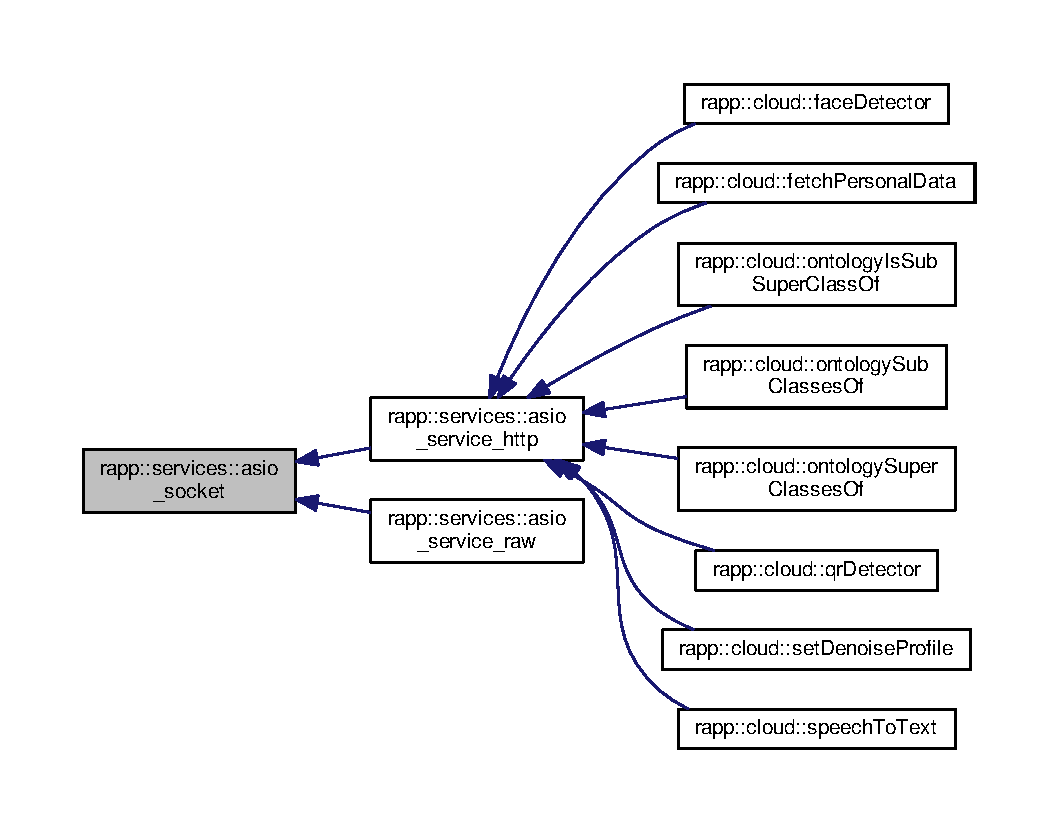
\includegraphics[width=350pt]{classrapp_1_1services_1_1asio__socket__inherit__graph}
\end{center}
\end{figure}
\subsection*{Public Member Functions}
\begin{DoxyCompactItemize}
\item 
virtual void \hyperlink{classrapp_1_1services_1_1asio__socket_a1241f0694fea6c2f13c361ddef13360b}{Schedule} (boost\-::asio\-::ip\-::tcp\-::resolver\-::query \&, boost\-::asio\-::ip\-::tcp\-::resolver \&, boost\-::asio\-::io\-\_\-service \&)=0
\end{DoxyCompactItemize}


\subsection{Detailed Description}
Abstract Base A\-S\-I\-O Socket class. 

Use for passing around the service controller, various types of sockets This Interface is needed, so that different services, can be passed to the scheduler transparently

\begin{DoxyVersion}{Version}
2 
\end{DoxyVersion}
\begin{DoxyDate}{Date}
26-\/\-April-\/2015 
\end{DoxyDate}
\begin{DoxyAuthor}{Author}
Alex Gkiokas \href{mailto:a.gkiokas@ortelio.co.uk}{\tt a.\-gkiokas@ortelio.\-co.\-uk} 
\end{DoxyAuthor}


Definition at line 19 of file asio\-\_\-socket.\-hpp.



\subsection{Member Function Documentation}
\hypertarget{classrapp_1_1services_1_1asio__socket_a1241f0694fea6c2f13c361ddef13360b}{\index{rapp\-::services\-::asio\-\_\-socket@{rapp\-::services\-::asio\-\_\-socket}!Schedule@{Schedule}}
\index{Schedule@{Schedule}!rapp::services::asio_socket@{rapp\-::services\-::asio\-\_\-socket}}
\subsubsection[{Schedule}]{\setlength{\rightskip}{0pt plus 5cm}virtual void rapp\-::services\-::asio\-\_\-socket\-::\-Schedule (
\begin{DoxyParamCaption}
\item[{boost\-::asio\-::ip\-::tcp\-::resolver\-::query \&}]{, }
\item[{boost\-::asio\-::ip\-::tcp\-::resolver \&}]{, }
\item[{boost\-::asio\-::io\-\_\-service \&}]{}
\end{DoxyParamCaption}
)\hspace{0.3cm}{\ttfamily [pure virtual]}}}\label{classrapp_1_1services_1_1asio__socket_a1241f0694fea6c2f13c361ddef13360b}
Schedule this client as a job for execution using 
\begin{DoxyParams}{Parameters}
{\em query} & defines the actual U\-R\-L/\-U\-R\-I \\
\hline
{\em resolver} & is the U\-R\-L/\-U\-R\-I resolver reference \\
\hline
{\em io\-\_\-service} & is the service queue on which this job will be scheduled to run \\
\hline
\end{DoxyParams}


Implemented in \hyperlink{classrapp_1_1services_1_1asio__service__raw_a11078ec812461792f81bca299db468ce}{rapp\-::services\-::asio\-\_\-service\-\_\-raw}, and \hyperlink{classrapp_1_1services_1_1asio__service__http_ad95e973eef8650c5bbc8b90a95feac76}{rapp\-::services\-::asio\-\_\-service\-\_\-http}.



The documentation for this class was generated from the following file\-:\begin{DoxyCompactItemize}
\item 
/home/travis/rapp\-\_\-temp/rapp-\/api/cpp/includes/service/asio\-\_\-socket/\hyperlink{asio__socket_8hpp}{asio\-\_\-socket.\-hpp}\end{DoxyCompactItemize}

\hypertarget{classrapp_1_1object_1_1audio}{\section{rapp\-:\-:object\-:\-:audio Class Reference}
\label{classrapp_1_1object_1_1audio}\index{rapp\-::object\-::audio@{rapp\-::object\-::audio}}
}


class which wraps around raw bytes of an audiofile  




{\ttfamily \#include $<$audio.\-hpp$>$}



Inheritance diagram for rapp\-:\-:object\-:\-:audio\-:
\nopagebreak
\begin{figure}[H]
\begin{center}
\leavevmode
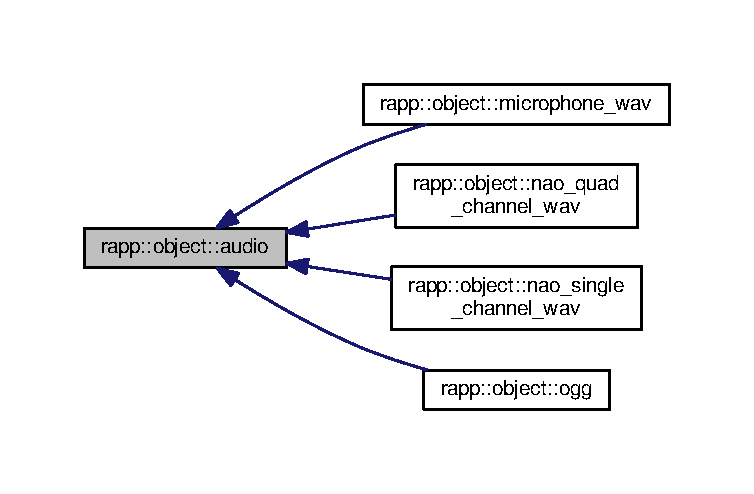
\includegraphics[width=350pt]{classrapp_1_1object_1_1audio__inherit__graph}
\end{center}
\end{figure}
\subsection*{Public Member Functions}
\begin{DoxyCompactItemize}
\item 
\hyperlink{classrapp_1_1object_1_1audio_a01c7492e030076cf3f579fee73990b96}{audio} (const std\-::string filepath)
\begin{DoxyCompactList}\small\item\em Construct from a file on disk. \end{DoxyCompactList}\item 
\hyperlink{classrapp_1_1object_1_1audio_a5f8b8dea6ffe4c30bb7af66244a3cd48}{audio} (std\-::ifstream \&bytestream)
\begin{DoxyCompactList}\small\item\em Construct using an open file stream. \end{DoxyCompactList}\item 
\hyperlink{classrapp_1_1object_1_1audio_af6cb71fb68efdfa45194b640d6076d94}{audio} (std\-::vector$<$ \hyperlink{namespacerapp_1_1types_a1dbc9dc2ab4507d8fb58ac3a204d307b}{rapp\-::types\-::byte} $>$ \hyperlink{classrapp_1_1object_1_1audio_aa2a7060842d1c1109ef2f0962c8351d4}{bytearray})
\begin{DoxyCompactList}\small\item\em construct using an existing byte-\/array \end{DoxyCompactList}\item 
\hyperlink{classrapp_1_1object_1_1audio_a55ba2b7c267b6e6ad168611d7141e239}{audio} (const \hyperlink{classrapp_1_1object_1_1audio}{audio} \&)=default
\begin{DoxyCompactList}\small\item\em Copy constructor. \end{DoxyCompactList}\item 
virtual std\-::string \hyperlink{classrapp_1_1object_1_1audio_a6eddc8038cd4fc4bff131175f7072893}{audio\-\_\-source} () const 
\item 
std\-::vector$<$ \hyperlink{namespacerapp_1_1types_a1dbc9dc2ab4507d8fb58ac3a204d307b}{rapp\-::types\-::byte} $>$ \hyperlink{classrapp_1_1object_1_1audio_aa2a7060842d1c1109ef2f0962c8351d4}{bytearray} () const 
\begin{DoxyCompactList}\small\item\em Get audio as array of bytes. \end{DoxyCompactList}\item 
virtual std\-::string \hyperlink{classrapp_1_1object_1_1audio_a7ee90cb61007fd9104e3349f5525ee47}{extension} () const 
\item 
\hyperlink{classrapp_1_1object_1_1audio}{audio} \& \hyperlink{classrapp_1_1object_1_1audio_a24f8fec829056bc30d9ec0fe0f23cac3}{operator=} (const \hyperlink{classrapp_1_1object_1_1audio}{audio} \&)=default
\begin{DoxyCompactList}\small\item\em Assignment operator. \end{DoxyCompactList}\item 
bool \hyperlink{classrapp_1_1object_1_1audio_ab8b7346c6154da6b265b904a1a23d576}{operator==} (const \hyperlink{classrapp_1_1object_1_1audio}{audio} \&rhs) const 
\begin{DoxyCompactList}\small\item\em Are audios same ? \end{DoxyCompactList}\item 
bool \hyperlink{classrapp_1_1object_1_1audio_a5181e49b76ea2e1de3e384faca2ec3e2}{save} (const std\-::string filepath)
\begin{DoxyCompactList}\small\item\em Save audio to filepath. \end{DoxyCompactList}\end{DoxyCompactItemize}
\subsection*{Private Member Functions}
\begin{DoxyCompactItemize}
\item 
\hyperlink{classrapp_1_1object_1_1audio_abd9bb56f1a4395059f8e2cde05e8a909}{audio} ()=delete
\item 
void \hyperlink{classrapp_1_1object_1_1audio_a528d4cbe9e092cdb8bfb293878c4717c}{read\-\_\-bytes} (std\-::ifstream \&bytestream)
\end{DoxyCompactItemize}
\subsection*{Private Attributes}
\begin{DoxyCompactItemize}
\item 
std\-::vector$<$ \hyperlink{namespacerapp_1_1types_a1dbc9dc2ab4507d8fb58ac3a204d307b}{rapp\-::types\-::byte} $>$ \hyperlink{classrapp_1_1object_1_1audio_a1ccd44fcbf55525739ef0c2f41de6878}{bytearray\-\_\-}
\end{DoxyCompactItemize}


\subsection{Detailed Description}
class which wraps around raw bytes of an audiofile 

\begin{DoxyVersion}{Version}
2 
\end{DoxyVersion}
\begin{DoxyDate}{Date}
January-\/2016 
\end{DoxyDate}
\begin{DoxyAuthor}{Author}
Alex Gkiokas \href{mailto:a.gkiokas@ortelio.co.uk}{\tt a.\-gkiokas@ortelio.\-co.\-uk} 
\end{DoxyAuthor}


Definition at line 13 of file audio.\-hpp.



\subsection{Constructor \& Destructor Documentation}
\hypertarget{classrapp_1_1object_1_1audio_a01c7492e030076cf3f579fee73990b96}{\index{rapp\-::object\-::audio@{rapp\-::object\-::audio}!audio@{audio}}
\index{audio@{audio}!rapp::object::audio@{rapp\-::object\-::audio}}
\subsubsection[{audio}]{\setlength{\rightskip}{0pt plus 5cm}rapp\-::object\-::audio\-::audio (
\begin{DoxyParamCaption}
\item[{const std\-::string}]{filepath}
\end{DoxyParamCaption}
)}}\label{classrapp_1_1object_1_1audio_a01c7492e030076cf3f579fee73990b96}


Construct from a file on disk. 



Definition at line 17 of file audio.\-hpp.

\hypertarget{classrapp_1_1object_1_1audio_a5f8b8dea6ffe4c30bb7af66244a3cd48}{\index{rapp\-::object\-::audio@{rapp\-::object\-::audio}!audio@{audio}}
\index{audio@{audio}!rapp::object::audio@{rapp\-::object\-::audio}}
\subsubsection[{audio}]{\setlength{\rightskip}{0pt plus 5cm}rapp\-::object\-::audio\-::audio (
\begin{DoxyParamCaption}
\item[{std\-::ifstream \&}]{bytestream}
\end{DoxyParamCaption}
)}}\label{classrapp_1_1object_1_1audio_a5f8b8dea6ffe4c30bb7af66244a3cd48}


Construct using an open file stream. 


\begin{DoxyParams}{Parameters}
{\em bytestream} & will be {\bfseries consumed} by the object \\
\hline
\end{DoxyParams}


Definition at line 33 of file audio.\-hpp.

\hypertarget{classrapp_1_1object_1_1audio_af6cb71fb68efdfa45194b640d6076d94}{\index{rapp\-::object\-::audio@{rapp\-::object\-::audio}!audio@{audio}}
\index{audio@{audio}!rapp::object::audio@{rapp\-::object\-::audio}}
\subsubsection[{audio}]{\setlength{\rightskip}{0pt plus 5cm}rapp\-::object\-::audio\-::audio (
\begin{DoxyParamCaption}
\item[{std\-::vector$<$ {\bf rapp\-::types\-::byte} $>$}]{bytearray}
\end{DoxyParamCaption}
)}}\label{classrapp_1_1object_1_1audio_af6cb71fb68efdfa45194b640d6076d94}


construct using an existing byte-\/array 


\begin{DoxyParams}{Parameters}
{\em bytearray} & should contain the audio data \\
\hline
\end{DoxyParams}


Definition at line 40 of file audio.\-hpp.

\hypertarget{classrapp_1_1object_1_1audio_a55ba2b7c267b6e6ad168611d7141e239}{\index{rapp\-::object\-::audio@{rapp\-::object\-::audio}!audio@{audio}}
\index{audio@{audio}!rapp::object::audio@{rapp\-::object\-::audio}}
\subsubsection[{audio}]{\setlength{\rightskip}{0pt plus 5cm}rapp\-::object\-::audio\-::audio (
\begin{DoxyParamCaption}
\item[{const {\bf audio} \&}]{}
\end{DoxyParamCaption}
)\hspace{0.3cm}{\ttfamily [default]}}}\label{classrapp_1_1object_1_1audio_a55ba2b7c267b6e6ad168611d7141e239}


Copy constructor. 

\hypertarget{classrapp_1_1object_1_1audio_abd9bb56f1a4395059f8e2cde05e8a909}{\index{rapp\-::object\-::audio@{rapp\-::object\-::audio}!audio@{audio}}
\index{audio@{audio}!rapp::object::audio@{rapp\-::object\-::audio}}
\subsubsection[{audio}]{\setlength{\rightskip}{0pt plus 5cm}rapp\-::object\-::audio\-::audio (
\begin{DoxyParamCaption}
{}
\end{DoxyParamCaption}
)\hspace{0.3cm}{\ttfamily [private]}, {\ttfamily [delete]}}}\label{classrapp_1_1object_1_1audio_abd9bb56f1a4395059f8e2cde05e8a909}


\subsection{Member Function Documentation}
\hypertarget{classrapp_1_1object_1_1audio_a6eddc8038cd4fc4bff131175f7072893}{\index{rapp\-::object\-::audio@{rapp\-::object\-::audio}!audio\-\_\-source@{audio\-\_\-source}}
\index{audio\-\_\-source@{audio\-\_\-source}!rapp::object::audio@{rapp\-::object\-::audio}}
\subsubsection[{audio\-\_\-source}]{\setlength{\rightskip}{0pt plus 5cm}virtual std\-::string rapp\-::object\-::audio\-::audio\-\_\-source (
\begin{DoxyParamCaption}
{}
\end{DoxyParamCaption}
) const\hspace{0.3cm}{\ttfamily [virtual]}}}\label{classrapp_1_1object_1_1audio_a6eddc8038cd4fc4bff131175f7072893}


Reimplemented in \hyperlink{classrapp_1_1object_1_1microphone__wav_a2342026e444e5cc08d31c4be598f7802}{rapp\-::object\-::microphone\-\_\-wav}, \hyperlink{classrapp_1_1object_1_1nao__quad__channel__wav_ade8c246f19eed5111d5946daeebec5ca}{rapp\-::object\-::nao\-\_\-quad\-\_\-channel\-\_\-wav}, \hyperlink{classrapp_1_1object_1_1nao__single__channel__wav_ab2f2352541061e3f4d66e549a588c197}{rapp\-::object\-::nao\-\_\-single\-\_\-channel\-\_\-wav}, and \hyperlink{classrapp_1_1object_1_1ogg_aa90df9567b6e09fef51d3c7f60df9d39}{rapp\-::object\-::ogg}.



Definition at line 78 of file audio.\-hpp.

\hypertarget{classrapp_1_1object_1_1audio_aa2a7060842d1c1109ef2f0962c8351d4}{\index{rapp\-::object\-::audio@{rapp\-::object\-::audio}!bytearray@{bytearray}}
\index{bytearray@{bytearray}!rapp::object::audio@{rapp\-::object\-::audio}}
\subsubsection[{bytearray}]{\setlength{\rightskip}{0pt plus 5cm}std\-::vector$<${\bf rapp\-::types\-::byte}$>$ rapp\-::object\-::audio\-::bytearray (
\begin{DoxyParamCaption}
{}
\end{DoxyParamCaption}
) const}}\label{classrapp_1_1object_1_1audio_aa2a7060842d1c1109ef2f0962c8351d4}


Get audio as array of bytes. 



Definition at line 48 of file audio.\-hpp.

\hypertarget{classrapp_1_1object_1_1audio_a7ee90cb61007fd9104e3349f5525ee47}{\index{rapp\-::object\-::audio@{rapp\-::object\-::audio}!extension@{extension}}
\index{extension@{extension}!rapp::object::audio@{rapp\-::object\-::audio}}
\subsubsection[{extension}]{\setlength{\rightskip}{0pt plus 5cm}virtual std\-::string rapp\-::object\-::audio\-::extension (
\begin{DoxyParamCaption}
{}
\end{DoxyParamCaption}
) const\hspace{0.3cm}{\ttfamily [virtual]}}}\label{classrapp_1_1object_1_1audio_a7ee90cb61007fd9104e3349f5525ee47}


Reimplemented in \hyperlink{classrapp_1_1object_1_1microphone__wav_aa6bd3fcfba97df55ef01ac41eb8ea65f}{rapp\-::object\-::microphone\-\_\-wav}, \hyperlink{classrapp_1_1object_1_1nao__quad__channel__wav_adb9adb9f8704b1ac1ac8fd9d7148e5b8}{rapp\-::object\-::nao\-\_\-quad\-\_\-channel\-\_\-wav}, \hyperlink{classrapp_1_1object_1_1nao__single__channel__wav_a747c61b5de738b34f7a8bd549775bb57}{rapp\-::object\-::nao\-\_\-single\-\_\-channel\-\_\-wav}, and \hyperlink{classrapp_1_1object_1_1ogg_a58ef4781ddac8bfe114c8b7f2c12ebed}{rapp\-::object\-::ogg}.



Definition at line 81 of file audio.\-hpp.

\hypertarget{classrapp_1_1object_1_1audio_a24f8fec829056bc30d9ec0fe0f23cac3}{\index{rapp\-::object\-::audio@{rapp\-::object\-::audio}!operator=@{operator=}}
\index{operator=@{operator=}!rapp::object::audio@{rapp\-::object\-::audio}}
\subsubsection[{operator=}]{\setlength{\rightskip}{0pt plus 5cm}{\bf audio}\& rapp\-::object\-::audio\-::operator= (
\begin{DoxyParamCaption}
\item[{const {\bf audio} \&}]{}
\end{DoxyParamCaption}
)\hspace{0.3cm}{\ttfamily [default]}}}\label{classrapp_1_1object_1_1audio_a24f8fec829056bc30d9ec0fe0f23cac3}


Assignment operator. 

\hypertarget{classrapp_1_1object_1_1audio_ab8b7346c6154da6b265b904a1a23d576}{\index{rapp\-::object\-::audio@{rapp\-::object\-::audio}!operator==@{operator==}}
\index{operator==@{operator==}!rapp::object::audio@{rapp\-::object\-::audio}}
\subsubsection[{operator==}]{\setlength{\rightskip}{0pt plus 5cm}bool rapp\-::object\-::audio\-::operator== (
\begin{DoxyParamCaption}
\item[{const {\bf audio} \&}]{rhs}
\end{DoxyParamCaption}
) const}}\label{classrapp_1_1object_1_1audio_ab8b7346c6154da6b265b904a1a23d576}


Are audios same ? 



Definition at line 54 of file audio.\-hpp.

\hypertarget{classrapp_1_1object_1_1audio_a528d4cbe9e092cdb8bfb293878c4717c}{\index{rapp\-::object\-::audio@{rapp\-::object\-::audio}!read\-\_\-bytes@{read\-\_\-bytes}}
\index{read\-\_\-bytes@{read\-\_\-bytes}!rapp::object::audio@{rapp\-::object\-::audio}}
\subsubsection[{read\-\_\-bytes}]{\setlength{\rightskip}{0pt plus 5cm}void rapp\-::object\-::audio\-::read\-\_\-bytes (
\begin{DoxyParamCaption}
\item[{std\-::ifstream \&}]{bytestream}
\end{DoxyParamCaption}
)\hspace{0.3cm}{\ttfamily [private]}}}\label{classrapp_1_1object_1_1audio_a528d4cbe9e092cdb8bfb293878c4717c}


Definition at line 90 of file audio.\-hpp.

\hypertarget{classrapp_1_1object_1_1audio_a5181e49b76ea2e1de3e384faca2ec3e2}{\index{rapp\-::object\-::audio@{rapp\-::object\-::audio}!save@{save}}
\index{save@{save}!rapp::object::audio@{rapp\-::object\-::audio}}
\subsubsection[{save}]{\setlength{\rightskip}{0pt plus 5cm}bool rapp\-::object\-::audio\-::save (
\begin{DoxyParamCaption}
\item[{const std\-::string}]{filepath}
\end{DoxyParamCaption}
)}}\label{classrapp_1_1object_1_1audio_a5181e49b76ea2e1de3e384faca2ec3e2}


Save audio to filepath. 



Definition at line 64 of file audio.\-hpp.



\subsection{Member Data Documentation}
\hypertarget{classrapp_1_1object_1_1audio_a1ccd44fcbf55525739ef0c2f41de6878}{\index{rapp\-::object\-::audio@{rapp\-::object\-::audio}!bytearray\-\_\-@{bytearray\-\_\-}}
\index{bytearray\-\_\-@{bytearray\-\_\-}!rapp::object::audio@{rapp\-::object\-::audio}}
\subsubsection[{bytearray\-\_\-}]{\setlength{\rightskip}{0pt plus 5cm}std\-::vector$<${\bf rapp\-::types\-::byte}$>$ rapp\-::object\-::audio\-::bytearray\-\_\-\hspace{0.3cm}{\ttfamily [private]}}}\label{classrapp_1_1object_1_1audio_a1ccd44fcbf55525739ef0c2f41de6878}


Definition at line 100 of file audio.\-hpp.



The documentation for this class was generated from the following file\-:\begin{DoxyCompactItemize}
\item 
/home/travis/rapp\-\_\-temp/rapp-\/api/cpp/includes/objects/audio/\hyperlink{audio_8hpp}{audio.\-hpp}\end{DoxyCompactItemize}

\hypertarget{classRappCloud_1_1CloudInterface_1_1CloudInterface_1_1CloudInterface}{\section{Rapp\-Cloud.\-Cloud\-Interface.\-Cloud\-Interface.\-Cloud\-Interface Class Reference}
\label{classRappCloud_1_1CloudInterface_1_1CloudInterface_1_1CloudInterface}\index{Rapp\-Cloud.\-Cloud\-Interface.\-Cloud\-Interface.\-Cloud\-Interface@{Rapp\-Cloud.\-Cloud\-Interface.\-Cloud\-Interface.\-Cloud\-Interface}}
}


Cloud Interface class.  


\subsection*{Static Public Member Functions}
\begin{DoxyCompactItemize}
\item 
def \hyperlink{classRappCloud_1_1CloudInterface_1_1CloudInterface_1_1CloudInterface_a65afc3f6348cecf7ea910e7500d6216d}{call\-Service}
\begin{DoxyCompactList}\small\item\em Performs Platform's H\-O\-P Web Service request. \end{DoxyCompactList}\item 
def \hyperlink{classRappCloud_1_1CloudInterface_1_1CloudInterface_1_1CloudInterface_a9789e50a5ecd0978f7ea9d9fdef75c48}{is\-Json}
\begin{DoxyCompactList}\small\item\em Check if an object (literal) is in json representation format. \end{DoxyCompactList}\end{DoxyCompactItemize}


\subsection{Detailed Description}
Cloud Interface class. 

Service controller for H\-O\-P Web Services requests Static class. 

Definition at line 41 of file Cloud\-Interface.\-py.



\subsection{Member Function Documentation}
\hypertarget{classRappCloud_1_1CloudInterface_1_1CloudInterface_1_1CloudInterface_a65afc3f6348cecf7ea910e7500d6216d}{\index{Rapp\-Cloud\-::\-Cloud\-Interface\-::\-Cloud\-Interface\-::\-Cloud\-Interface@{Rapp\-Cloud\-::\-Cloud\-Interface\-::\-Cloud\-Interface\-::\-Cloud\-Interface}!call\-Service@{call\-Service}}
\index{call\-Service@{call\-Service}!RappCloud::CloudInterface::CloudInterface::CloudInterface@{Rapp\-Cloud\-::\-Cloud\-Interface\-::\-Cloud\-Interface\-::\-Cloud\-Interface}}
\subsubsection[{call\-Service}]{\setlength{\rightskip}{0pt plus 5cm}def Rapp\-Cloud.\-Cloud\-Interface.\-Cloud\-Interface.\-Cloud\-Interface.\-call\-Service (
\begin{DoxyParamCaption}
\item[{}]{url, }
\item[{}]{payload, }
\item[{}]{files, }
\item[{}]{basic\-Auth}
\end{DoxyParamCaption}
)\hspace{0.3cm}{\ttfamily [static]}}}\label{classRappCloud_1_1CloudInterface_1_1CloudInterface_1_1CloudInterface_a65afc3f6348cecf7ea910e7500d6216d}


Performs Platform's H\-O\-P Web Service request. 


\begin{DoxyParams}{Parameters}
{\em basic\-Auth} & Basic http authentication credentials \{'username'\-: '', 'password'\-: ''\} \\
\hline
{\em url} & Post request destination Url. \\
\hline
{\em payload} & data payload of the post request. \\
\hline
{\em files} & multipart post file field.\\
\hline
\end{DoxyParams}
\begin{DoxyReturn}{Returns}
Rapp Platform Service response object. 
\end{DoxyReturn}


Definition at line 54 of file Cloud\-Interface.\-py.

\hypertarget{classRappCloud_1_1CloudInterface_1_1CloudInterface_1_1CloudInterface_a9789e50a5ecd0978f7ea9d9fdef75c48}{\index{Rapp\-Cloud\-::\-Cloud\-Interface\-::\-Cloud\-Interface\-::\-Cloud\-Interface@{Rapp\-Cloud\-::\-Cloud\-Interface\-::\-Cloud\-Interface\-::\-Cloud\-Interface}!is\-Json@{is\-Json}}
\index{is\-Json@{is\-Json}!RappCloud::CloudInterface::CloudInterface::CloudInterface@{Rapp\-Cloud\-::\-Cloud\-Interface\-::\-Cloud\-Interface\-::\-Cloud\-Interface}}
\subsubsection[{is\-Json}]{\setlength{\rightskip}{0pt plus 5cm}def Rapp\-Cloud.\-Cloud\-Interface.\-Cloud\-Interface.\-Cloud\-Interface.\-is\-Json (
\begin{DoxyParamCaption}
\item[{}]{obj}
\end{DoxyParamCaption}
)\hspace{0.3cm}{\ttfamily [static]}}}\label{classRappCloud_1_1CloudInterface_1_1CloudInterface_1_1CloudInterface_a9789e50a5ecd0978f7ea9d9fdef75c48}


Check if an object (literal) is in json representation format. 


\begin{DoxyParams}{Parameters}
{\em obj} & Object (literal).\\
\hline
\end{DoxyParams}
\begin{DoxyReturn}{Returns}
True if object is a json object. False otherwise. 
\end{DoxyReturn}


Definition at line 105 of file Cloud\-Interface.\-py.



The documentation for this class was generated from the following file\-:\begin{DoxyCompactItemize}
\item 
/home/travis/rapp\-\_\-temp/rapp-\/api/python/\-Rapp\-Cloud/\-Cloud\-Interface/\hyperlink{CloudInterface_8py}{Cloud\-Interface.\-py}\end{DoxyCompactItemize}

\hypertarget{classrapp_1_1robot_1_1communication}{\section{rapp\-:\-:robot\-:\-:communication Class Reference}
\label{classrapp_1_1robot_1_1communication}\index{rapp\-::robot\-::communication@{rapp\-::robot\-::communication}}
}


Abstract Base Class (A\-B\-C) Interface for Robot Communication.  




{\ttfamily \#include $<$communication.\-hpp$>$}

\subsection*{Public Types}
\begin{DoxyCompactItemize}
\item 
enum \hyperlink{classrapp_1_1robot_1_1communication_aa68950f71c5f18df6816725b50c3c62e}{Language} \{ \\*
\hyperlink{classrapp_1_1robot_1_1communication_aa68950f71c5f18df6816725b50c3c62ea11040bd29db4ec9964af9fd3f9a24f17}{Language\-::\-E\-N\-G\-L\-I\-S\-H}, 
\\*
\hyperlink{classrapp_1_1robot_1_1communication_aa68950f71c5f18df6816725b50c3c62ead4cacc28e56302bcec9d7af4bba8c9a7}{Language\-::\-G\-R\-E\-E\-K}
 \}
\end{DoxyCompactItemize}
\subsection*{Public Member Functions}
\begin{DoxyCompactItemize}
\item 
virtual bool \hyperlink{classrapp_1_1robot_1_1communication_ab33428a7ba5c82056fe5942efbd2ce2d}{capture\-Audio} (std\-::shared\-\_\-ptr$<$ \hyperlink{classrapp_1_1object_1_1audio}{rapp\-:object\-::audio} $>$ buffer, float waiting\-\_\-time, float microphone\-\_\-energy)=0
\begin{DoxyCompactList}\small\item\em Record audio. \end{DoxyCompactList}\item 
virtual bool \hyperlink{classrapp_1_1robot_1_1communication_ab38cea79d2b7fdeecdeebf02ddad3341}{play\-Audio} (const std\-::string \&file\-\_\-path, double position, double volume, double balance, bool play\-\_\-in\-\_\-loop)=0
\begin{DoxyCompactList}\small\item\em Produce Audio from robot's speakers. \end{DoxyCompactList}\item 
virtual bool \hyperlink{classrapp_1_1robot_1_1communication_a04d8ae71d953aa66a4c00149548ad750}{text\-To\-Speech} (const std\-::string str, \hyperlink{classrapp_1_1robot_1_1communication_aa68950f71c5f18df6816725b50c3c62e}{Language} language=\hyperlink{classrapp_1_1robot_1_1communication_aa68950f71c5f18df6816725b50c3c62ea11040bd29db4ec9964af9fd3f9a24f17}{Language\-::\-E\-N\-G\-L\-I\-S\-H})=0
\begin{DoxyCompactList}\small\item\em Produce speec from text. \end{DoxyCompactList}\item 
virtual std\-::string \hyperlink{classrapp_1_1robot_1_1communication_aeddb446d64faad99717229870caa9927}{word\-Spotting} (std\-::array$<$ std\-::string $>$ dictionary, unsigned int size)=0
\begin{DoxyCompactList}\small\item\em ? \end{DoxyCompactList}\end{DoxyCompactItemize}
\begin{Indent}{\bf used for?}\par
{\em Get Microphone Energy -\/ N\-O\-T\-E what is the Param }\begin{DoxyCompactItemize}
\item 
virtual float \hyperlink{classrapp_1_1robot_1_1communication_a8baa4b3616a74e22bbf0455122eb695d}{get\-Microphone\-Energy} (std\-::string name) const =0
\item 
virtual bool \hyperlink{classrapp_1_1robot_1_1communication_ac47da76d51faee1744d0521e1f7aac25}{voice\-Record} (const std\-::shared\-\_\-ptr$<$ \hyperlink{classrapp_1_1object_1_1audio}{rapp\-::object\-::audio} $>$)=0
\end{DoxyCompactItemize}
\end{Indent}


\subsection{Detailed Description}
Abstract Base Class (A\-B\-C) Interface for Robot Communication. 

\begin{DoxyVersion}{Version}
1 
\end{DoxyVersion}
\begin{DoxyDate}{Date}
20-\/\-September-\/2015 
\end{DoxyDate}
\begin{DoxyAuthor}{Author}
Alex Giokas \href{mailto:a.gkiokas@ortelio.co.uk}{\tt a.\-gkiokas@ortelio.\-co.\-uk}
\end{DoxyAuthor}
This class specifies the interface for all communications. It is your responsibility to implement them appropriately. 

Definition at line 16 of file communication.\-hpp.



\subsection{Member Enumeration Documentation}
\hypertarget{classrapp_1_1robot_1_1communication_aa68950f71c5f18df6816725b50c3c62e}{\index{rapp\-::robot\-::communication@{rapp\-::robot\-::communication}!Language@{Language}}
\index{Language@{Language}!rapp::robot::communication@{rapp\-::robot\-::communication}}
\subsubsection[{Language}]{\setlength{\rightskip}{0pt plus 5cm}enum {\bf rapp\-::robot\-::communication\-::\-Language}\hspace{0.3cm}{\ttfamily [strong]}}}\label{classrapp_1_1robot_1_1communication_aa68950f71c5f18df6816725b50c3c62e}
\begin{Desc}
\item[Enumerator]\par
\begin{description}
\index{E\-N\-G\-L\-I\-S\-H@{E\-N\-G\-L\-I\-S\-H}!rapp\-::robot\-::communication@{rapp\-::robot\-::communication}}\index{rapp\-::robot\-::communication@{rapp\-::robot\-::communication}!E\-N\-G\-L\-I\-S\-H@{E\-N\-G\-L\-I\-S\-H}}\item[{\em 
\hypertarget{classrapp_1_1robot_1_1communication_aa68950f71c5f18df6816725b50c3c62ea11040bd29db4ec9964af9fd3f9a24f17}{E\-N\-G\-L\-I\-S\-H}\label{classrapp_1_1robot_1_1communication_aa68950f71c5f18df6816725b50c3c62ea11040bd29db4ec9964af9fd3f9a24f17}
}]\index{G\-R\-E\-E\-K@{G\-R\-E\-E\-K}!rapp\-::robot\-::communication@{rapp\-::robot\-::communication}}\index{rapp\-::robot\-::communication@{rapp\-::robot\-::communication}!G\-R\-E\-E\-K@{G\-R\-E\-E\-K}}\item[{\em 
\hypertarget{classrapp_1_1robot_1_1communication_aa68950f71c5f18df6816725b50c3c62ead4cacc28e56302bcec9d7af4bba8c9a7}{G\-R\-E\-E\-K}\label{classrapp_1_1robot_1_1communication_aa68950f71c5f18df6816725b50c3c62ead4cacc28e56302bcec9d7af4bba8c9a7}
}]\end{description}
\end{Desc}


Definition at line 20 of file communication.\-hpp.



\subsection{Member Function Documentation}
\hypertarget{classrapp_1_1robot_1_1communication_ab33428a7ba5c82056fe5942efbd2ce2d}{\index{rapp\-::robot\-::communication@{rapp\-::robot\-::communication}!capture\-Audio@{capture\-Audio}}
\index{capture\-Audio@{capture\-Audio}!rapp::robot::communication@{rapp\-::robot\-::communication}}
\subsubsection[{capture\-Audio}]{\setlength{\rightskip}{0pt plus 5cm}virtual bool rapp\-::robot\-::communication\-::capture\-Audio (
\begin{DoxyParamCaption}
\item[{std\-::shared\-\_\-ptr$<$ {\bf rapp\-:object\-::audio} $>$}]{buffer, }
\item[{float}]{waiting\-\_\-time, }
\item[{float}]{microphone\-\_\-energy}
\end{DoxyParamCaption}
)\hspace{0.3cm}{\ttfamily [pure virtual]}}}\label{classrapp_1_1robot_1_1communication_ab33428a7ba5c82056fe5942efbd2ce2d}


Record audio. 

\hypertarget{classrapp_1_1robot_1_1communication_a8baa4b3616a74e22bbf0455122eb695d}{\index{rapp\-::robot\-::communication@{rapp\-::robot\-::communication}!get\-Microphone\-Energy@{get\-Microphone\-Energy}}
\index{get\-Microphone\-Energy@{get\-Microphone\-Energy}!rapp::robot::communication@{rapp\-::robot\-::communication}}
\subsubsection[{get\-Microphone\-Energy}]{\setlength{\rightskip}{0pt plus 5cm}virtual float rapp\-::robot\-::communication\-::get\-Microphone\-Energy (
\begin{DoxyParamCaption}
\item[{std\-::string}]{name}
\end{DoxyParamCaption}
) const\hspace{0.3cm}{\ttfamily [pure virtual]}}}\label{classrapp_1_1robot_1_1communication_a8baa4b3616a74e22bbf0455122eb695d}
\hypertarget{classrapp_1_1robot_1_1communication_ab38cea79d2b7fdeecdeebf02ddad3341}{\index{rapp\-::robot\-::communication@{rapp\-::robot\-::communication}!play\-Audio@{play\-Audio}}
\index{play\-Audio@{play\-Audio}!rapp::robot::communication@{rapp\-::robot\-::communication}}
\subsubsection[{play\-Audio}]{\setlength{\rightskip}{0pt plus 5cm}virtual bool rapp\-::robot\-::communication\-::play\-Audio (
\begin{DoxyParamCaption}
\item[{const std\-::string \&}]{file\-\_\-path, }
\item[{double}]{position, }
\item[{double}]{volume, }
\item[{double}]{balance, }
\item[{bool}]{play\-\_\-in\-\_\-loop}
\end{DoxyParamCaption}
)\hspace{0.3cm}{\ttfamily [pure virtual]}}}\label{classrapp_1_1robot_1_1communication_ab38cea79d2b7fdeecdeebf02ddad3341}


Produce Audio from robot's speakers. 

\hypertarget{classrapp_1_1robot_1_1communication_a04d8ae71d953aa66a4c00149548ad750}{\index{rapp\-::robot\-::communication@{rapp\-::robot\-::communication}!text\-To\-Speech@{text\-To\-Speech}}
\index{text\-To\-Speech@{text\-To\-Speech}!rapp::robot::communication@{rapp\-::robot\-::communication}}
\subsubsection[{text\-To\-Speech}]{\setlength{\rightskip}{0pt plus 5cm}virtual bool rapp\-::robot\-::communication\-::text\-To\-Speech (
\begin{DoxyParamCaption}
\item[{const std\-::string}]{str, }
\item[{{\bf Language}}]{language = {\ttfamily {\bf Language\-::\-E\-N\-G\-L\-I\-S\-H}}}
\end{DoxyParamCaption}
)\hspace{0.3cm}{\ttfamily [pure virtual]}}}\label{classrapp_1_1robot_1_1communication_a04d8ae71d953aa66a4c00149548ad750}


Produce speec from text. 

\hypertarget{classrapp_1_1robot_1_1communication_ac47da76d51faee1744d0521e1f7aac25}{\index{rapp\-::robot\-::communication@{rapp\-::robot\-::communication}!voice\-Record@{voice\-Record}}
\index{voice\-Record@{voice\-Record}!rapp::robot::communication@{rapp\-::robot\-::communication}}
\subsubsection[{voice\-Record}]{\setlength{\rightskip}{0pt plus 5cm}virtual bool rapp\-::robot\-::communication\-::voice\-Record (
\begin{DoxyParamCaption}
\item[{const std\-::shared\-\_\-ptr$<$ {\bf rapp\-::object\-::audio} $>$}]{}
\end{DoxyParamCaption}
)\hspace{0.3cm}{\ttfamily [pure virtual]}}}\label{classrapp_1_1robot_1_1communication_ac47da76d51faee1744d0521e1f7aac25}
Record Voice -\/ N\-O\-T\-E\-: 
\begin{DoxyParams}{Parameters}
{\em audio} & pointer will be updated If this method is asynchronous or multi-\/threaded, then you need to lock the pointer in your implementation. \\
\hline
\end{DoxyParams}
\hypertarget{classrapp_1_1robot_1_1communication_aeddb446d64faad99717229870caa9927}{\index{rapp\-::robot\-::communication@{rapp\-::robot\-::communication}!word\-Spotting@{word\-Spotting}}
\index{word\-Spotting@{word\-Spotting}!rapp::robot::communication@{rapp\-::robot\-::communication}}
\subsubsection[{word\-Spotting}]{\setlength{\rightskip}{0pt plus 5cm}virtual std\-::string rapp\-::robot\-::communication\-::word\-Spotting (
\begin{DoxyParamCaption}
\item[{std\-::array$<$ std\-::string $>$}]{dictionary, }
\item[{unsigned int}]{size}
\end{DoxyParamCaption}
)\hspace{0.3cm}{\ttfamily [pure virtual]}}}\label{classrapp_1_1robot_1_1communication_aeddb446d64faad99717229870caa9927}


? 



The documentation for this class was generated from the following file\-:\begin{DoxyCompactItemize}
\item 
/home/travis/rapp\-\_\-temp/rapp-\/api/cpp/includes/robot/communication/\hyperlink{communication_8hpp}{communication.\-hpp}\end{DoxyCompactItemize}

\hypertarget{classrapp_1_1object_1_1face}{\section{rapp\-:\-:object\-:\-:face Class Reference}
\label{classrapp_1_1object_1_1face}\index{rapp\-::object\-::face@{rapp\-::object\-::face}}
}


{\ttfamily \#include $<$face.\-hpp$>$}

\subsection*{Public Member Functions}
\begin{DoxyCompactItemize}
\item 
\hyperlink{classrapp_1_1object_1_1face_ab69a3ccafd0519c4c4a72af1142b4b07}{face} (float top\-\_\-left\-\_\-x, float top\-\_\-left\-\_\-y, float top\-\_\-left\-\_\-z, float bottom\-\_\-right\-\_\-x, float bottom\-\_\-right\-\_\-y, float bottom\-\_\-right\-\_\-z)
\begin{DoxyCompactList}\small\item\em Consruct using face coordinates (a rectangle) \end{DoxyCompactList}\item 
\hyperlink{classrapp_1_1object_1_1face_a94a6ba1f4f7e3e8b1398d5dbdd76acc9}{face} ()=default
\item 
\hyperlink{classrapp_1_1object_1_1face_a10fb28c9941145226e99111e73ed21ac}{face} (const \hyperlink{classrapp_1_1object_1_1face}{face} \&)=default
\begin{DoxyCompactList}\small\item\em Copy constructor. \end{DoxyCompactList}\item 
bool \hyperlink{classrapp_1_1object_1_1face_a8f1e247f980687e40969c159e7308ecd}{operator==} (const \hyperlink{classrapp_1_1object_1_1face}{face} \&rhs) const 
\begin{DoxyCompactList}\small\item\em Assignment Constructor. \end{DoxyCompactList}\end{DoxyCompactItemize}
\subsection*{Private Attributes}
\begin{DoxyCompactItemize}
\item 
float \hyperlink{classrapp_1_1object_1_1face_afc08b0adb766ef20c60bcd8c21d07852}{bottom\-\_\-right\-\_\-x\-\_\-\-\_\-} = -\/1.
\item 
float \hyperlink{classrapp_1_1object_1_1face_a228058127dbd3077c97edbed509865b8}{bottom\-\_\-right\-\_\-y\-\_\-\-\_\-} = -\/1.
\item 
float \hyperlink{classrapp_1_1object_1_1face_aa2e04032673a342f092f3a47a2419505}{bottom\-\_\-right\-\_\-z\-\_\-\-\_\-} = -\/1.
\item 
float \hyperlink{classrapp_1_1object_1_1face_a9d04cd084b62af674516aa71b8c8a142}{top\-\_\-left\-\_\-x\-\_\-\-\_\-} = -\/1.
\item 
float \hyperlink{classrapp_1_1object_1_1face_a49bd8f68f0c9a4a6dd14c315edc72d50}{top\-\_\-left\-\_\-y\-\_\-\-\_\-} = -\/1.
\item 
float \hyperlink{classrapp_1_1object_1_1face_ac11e89d2ed6a03ba5112a5a2ba308c56}{top\-\_\-left\-\_\-z\-\_\-\-\_\-} = -\/1.
\end{DoxyCompactItemize}


\subsection{Detailed Description}


Definition at line 16 of file face.\-hpp.



\subsection{Constructor \& Destructor Documentation}
\hypertarget{classrapp_1_1object_1_1face_ab69a3ccafd0519c4c4a72af1142b4b07}{\index{rapp\-::object\-::face@{rapp\-::object\-::face}!face@{face}}
\index{face@{face}!rapp::object::face@{rapp\-::object\-::face}}
\subsubsection[{face}]{\setlength{\rightskip}{0pt plus 5cm}rapp\-::object\-::face\-::face (
\begin{DoxyParamCaption}
\item[{float}]{top\-\_\-left\-\_\-x, }
\item[{float}]{top\-\_\-left\-\_\-y, }
\item[{float}]{top\-\_\-left\-\_\-z, }
\item[{float}]{bottom\-\_\-right\-\_\-x, }
\item[{float}]{bottom\-\_\-right\-\_\-y, }
\item[{float}]{bottom\-\_\-right\-\_\-z}
\end{DoxyParamCaption}
)}}\label{classrapp_1_1object_1_1face_ab69a3ccafd0519c4c4a72af1142b4b07}


Consruct using face coordinates (a rectangle) 



Definition at line 23 of file face.\-hpp.

\hypertarget{classrapp_1_1object_1_1face_a94a6ba1f4f7e3e8b1398d5dbdd76acc9}{\index{rapp\-::object\-::face@{rapp\-::object\-::face}!face@{face}}
\index{face@{face}!rapp::object::face@{rapp\-::object\-::face}}
\subsubsection[{face}]{\setlength{\rightskip}{0pt plus 5cm}rapp\-::object\-::face\-::face (
\begin{DoxyParamCaption}
{}
\end{DoxyParamCaption}
)\hspace{0.3cm}{\ttfamily [default]}}}\label{classrapp_1_1object_1_1face_a94a6ba1f4f7e3e8b1398d5dbdd76acc9}
\hypertarget{classrapp_1_1object_1_1face_a10fb28c9941145226e99111e73ed21ac}{\index{rapp\-::object\-::face@{rapp\-::object\-::face}!face@{face}}
\index{face@{face}!rapp::object::face@{rapp\-::object\-::face}}
\subsubsection[{face}]{\setlength{\rightskip}{0pt plus 5cm}rapp\-::object\-::face\-::face (
\begin{DoxyParamCaption}
\item[{const {\bf face} \&}]{}
\end{DoxyParamCaption}
)\hspace{0.3cm}{\ttfamily [default]}}}\label{classrapp_1_1object_1_1face_a10fb28c9941145226e99111e73ed21ac}


Copy constructor. 



\subsection{Member Function Documentation}
\hypertarget{classrapp_1_1object_1_1face_a8f1e247f980687e40969c159e7308ecd}{\index{rapp\-::object\-::face@{rapp\-::object\-::face}!operator==@{operator==}}
\index{operator==@{operator==}!rapp::object::face@{rapp\-::object\-::face}}
\subsubsection[{operator==}]{\setlength{\rightskip}{0pt plus 5cm}bool rapp\-::object\-::face\-::operator== (
\begin{DoxyParamCaption}
\item[{const {\bf face} \&}]{rhs}
\end{DoxyParamCaption}
) const}}\label{classrapp_1_1object_1_1face_a8f1e247f980687e40969c159e7308ecd}


Assignment Constructor. 

Equality operator 

Definition at line 49 of file face.\-hpp.



\subsection{Member Data Documentation}
\hypertarget{classrapp_1_1object_1_1face_afc08b0adb766ef20c60bcd8c21d07852}{\index{rapp\-::object\-::face@{rapp\-::object\-::face}!bottom\-\_\-right\-\_\-x\-\_\-\-\_\-@{bottom\-\_\-right\-\_\-x\-\_\-\-\_\-}}
\index{bottom\-\_\-right\-\_\-x\-\_\-\-\_\-@{bottom\-\_\-right\-\_\-x\-\_\-\-\_\-}!rapp::object::face@{rapp\-::object\-::face}}
\subsubsection[{bottom\-\_\-right\-\_\-x\-\_\-\-\_\-}]{\setlength{\rightskip}{0pt plus 5cm}float rapp\-::object\-::face\-::bottom\-\_\-right\-\_\-x\-\_\-\-\_\- = -\/1.\hspace{0.3cm}{\ttfamily [private]}}}\label{classrapp_1_1object_1_1face_afc08b0adb766ef20c60bcd8c21d07852}


Definition at line 64 of file face.\-hpp.

\hypertarget{classrapp_1_1object_1_1face_a228058127dbd3077c97edbed509865b8}{\index{rapp\-::object\-::face@{rapp\-::object\-::face}!bottom\-\_\-right\-\_\-y\-\_\-\-\_\-@{bottom\-\_\-right\-\_\-y\-\_\-\-\_\-}}
\index{bottom\-\_\-right\-\_\-y\-\_\-\-\_\-@{bottom\-\_\-right\-\_\-y\-\_\-\-\_\-}!rapp::object::face@{rapp\-::object\-::face}}
\subsubsection[{bottom\-\_\-right\-\_\-y\-\_\-\-\_\-}]{\setlength{\rightskip}{0pt plus 5cm}float rapp\-::object\-::face\-::bottom\-\_\-right\-\_\-y\-\_\-\-\_\- = -\/1.\hspace{0.3cm}{\ttfamily [private]}}}\label{classrapp_1_1object_1_1face_a228058127dbd3077c97edbed509865b8}


Definition at line 65 of file face.\-hpp.

\hypertarget{classrapp_1_1object_1_1face_aa2e04032673a342f092f3a47a2419505}{\index{rapp\-::object\-::face@{rapp\-::object\-::face}!bottom\-\_\-right\-\_\-z\-\_\-\-\_\-@{bottom\-\_\-right\-\_\-z\-\_\-\-\_\-}}
\index{bottom\-\_\-right\-\_\-z\-\_\-\-\_\-@{bottom\-\_\-right\-\_\-z\-\_\-\-\_\-}!rapp::object::face@{rapp\-::object\-::face}}
\subsubsection[{bottom\-\_\-right\-\_\-z\-\_\-\-\_\-}]{\setlength{\rightskip}{0pt plus 5cm}float rapp\-::object\-::face\-::bottom\-\_\-right\-\_\-z\-\_\-\-\_\- = -\/1.\hspace{0.3cm}{\ttfamily [private]}}}\label{classrapp_1_1object_1_1face_aa2e04032673a342f092f3a47a2419505}


Definition at line 66 of file face.\-hpp.

\hypertarget{classrapp_1_1object_1_1face_a9d04cd084b62af674516aa71b8c8a142}{\index{rapp\-::object\-::face@{rapp\-::object\-::face}!top\-\_\-left\-\_\-x\-\_\-\-\_\-@{top\-\_\-left\-\_\-x\-\_\-\-\_\-}}
\index{top\-\_\-left\-\_\-x\-\_\-\-\_\-@{top\-\_\-left\-\_\-x\-\_\-\-\_\-}!rapp::object::face@{rapp\-::object\-::face}}
\subsubsection[{top\-\_\-left\-\_\-x\-\_\-\-\_\-}]{\setlength{\rightskip}{0pt plus 5cm}float rapp\-::object\-::face\-::top\-\_\-left\-\_\-x\-\_\-\-\_\- = -\/1.\hspace{0.3cm}{\ttfamily [private]}}}\label{classrapp_1_1object_1_1face_a9d04cd084b62af674516aa71b8c8a142}


Definition at line 61 of file face.\-hpp.

\hypertarget{classrapp_1_1object_1_1face_a49bd8f68f0c9a4a6dd14c315edc72d50}{\index{rapp\-::object\-::face@{rapp\-::object\-::face}!top\-\_\-left\-\_\-y\-\_\-\-\_\-@{top\-\_\-left\-\_\-y\-\_\-\-\_\-}}
\index{top\-\_\-left\-\_\-y\-\_\-\-\_\-@{top\-\_\-left\-\_\-y\-\_\-\-\_\-}!rapp::object::face@{rapp\-::object\-::face}}
\subsubsection[{top\-\_\-left\-\_\-y\-\_\-\-\_\-}]{\setlength{\rightskip}{0pt plus 5cm}float rapp\-::object\-::face\-::top\-\_\-left\-\_\-y\-\_\-\-\_\- = -\/1.\hspace{0.3cm}{\ttfamily [private]}}}\label{classrapp_1_1object_1_1face_a49bd8f68f0c9a4a6dd14c315edc72d50}


Definition at line 62 of file face.\-hpp.

\hypertarget{classrapp_1_1object_1_1face_ac11e89d2ed6a03ba5112a5a2ba308c56}{\index{rapp\-::object\-::face@{rapp\-::object\-::face}!top\-\_\-left\-\_\-z\-\_\-\-\_\-@{top\-\_\-left\-\_\-z\-\_\-\-\_\-}}
\index{top\-\_\-left\-\_\-z\-\_\-\-\_\-@{top\-\_\-left\-\_\-z\-\_\-\-\_\-}!rapp::object::face@{rapp\-::object\-::face}}
\subsubsection[{top\-\_\-left\-\_\-z\-\_\-\-\_\-}]{\setlength{\rightskip}{0pt plus 5cm}float rapp\-::object\-::face\-::top\-\_\-left\-\_\-z\-\_\-\-\_\- = -\/1.\hspace{0.3cm}{\ttfamily [private]}}}\label{classrapp_1_1object_1_1face_ac11e89d2ed6a03ba5112a5a2ba308c56}


Definition at line 63 of file face.\-hpp.



The documentation for this class was generated from the following file\-:\begin{DoxyCompactItemize}
\item 
/home/travis/rapp\-\_\-temp/rapp-\/api/cpp/includes/objects/face/\hyperlink{face_8hpp}{face.\-hpp}\end{DoxyCompactItemize}

\hypertarget{classface}{\section{face Class Reference}
\label{classface}\index{face@{face}}
}


class which should somehow encapsulate a face  




{\ttfamily \#include $<$face.\-hpp$>$}



\subsection{Detailed Description}
class which should somehow encapsulate a face 

\begin{DoxyVersion}{Version}
1 
\end{DoxyVersion}
\begin{DoxyDate}{Date}
13-\/\-Feburary-\/2015 
\end{DoxyDate}
\begin{DoxyAuthor}{Author}
Alex Gkiokas \href{mailto:a.gkiokas@ortelio.co.uk}{\tt a.\-gkiokas@ortelio.\-co.\-uk} 
\end{DoxyAuthor}


The documentation for this class was generated from the following file\-:\begin{DoxyCompactItemize}
\item 
/home/travis/rapp\-\_\-temp/rapp-\/api/cpp/includes/objects/face/\hyperlink{face_8hpp}{face.\-hpp}\end{DoxyCompactItemize}

\hypertarget{classrapp_1_1cloud_1_1faceDetector}{\section{rapp\-:\-:cloud\-:\-:face\-Detector Class Reference}
\label{classrapp_1_1cloud_1_1faceDetector}\index{rapp\-::cloud\-::face\-Detector@{rapp\-::cloud\-::face\-Detector}}
}


Asynchronous Service which will request the cloud to detect faces.  




{\ttfamily \#include $<$face\-Detector.\-hpp$>$}



Inheritance diagram for rapp\-:\-:cloud\-:\-:face\-Detector\-:
\nopagebreak
\begin{figure}[H]
\begin{center}
\leavevmode
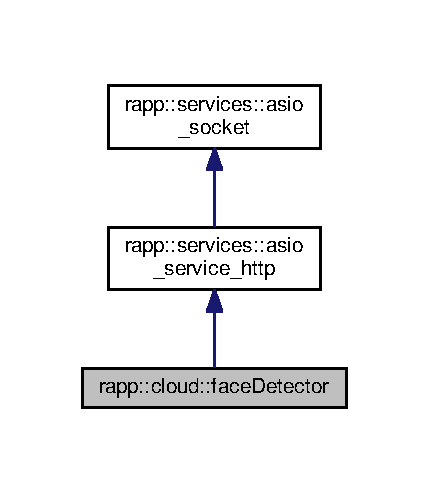
\includegraphics[width=206pt]{classrapp_1_1cloud_1_1faceDetector__inherit__graph}
\end{center}
\end{figure}


Collaboration diagram for rapp\-:\-:cloud\-:\-:face\-Detector\-:
\nopagebreak
\begin{figure}[H]
\begin{center}
\leavevmode
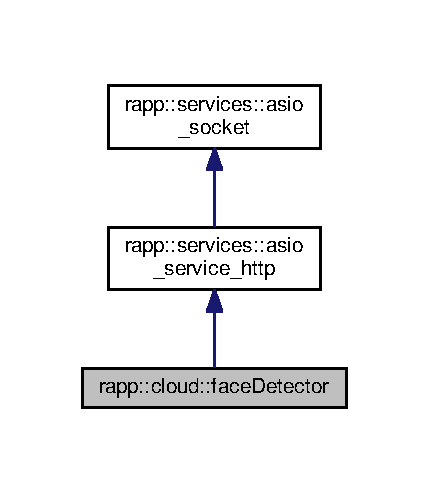
\includegraphics[width=206pt]{classrapp_1_1cloud_1_1faceDetector__coll__graph}
\end{center}
\end{figure}
\subsection*{Public Member Functions}
\begin{DoxyCompactItemize}
\item 
\hyperlink{classrapp_1_1cloud_1_1faceDetector_af693e139e042aaa52c235fcd768712bc}{face\-Detector} (const std\-::shared\-\_\-ptr$<$ \hyperlink{classrapp_1_1object_1_1picture}{rapp\-::object\-::picture} $>$ image, const std\-::string image\-\_\-format, std\-::function$<$ void(std\-::vector$<$ \hyperlink{classrapp_1_1object_1_1face}{rapp\-::object\-::face} $>$) $>$ callback)
\begin{DoxyCompactList}\small\item\em Constructor. \end{DoxyCompactList}\end{DoxyCompactItemize}
\subsection*{Private Member Functions}
\begin{DoxyCompactItemize}
\item 
void \hyperlink{classrapp_1_1cloud_1_1faceDetector_aa62da7d9f2fb7e45fabd5612ae139e46}{handle\-\_\-reply} (std\-::string json)
\end{DoxyCompactItemize}
\subsection*{Private Attributes}
\begin{DoxyCompactItemize}
\item 
std\-::function$<$ void(std\-::vector\\*
$<$ \hyperlink{classrapp_1_1object_1_1face}{rapp\-::object\-::face} $>$) $>$ \hyperlink{classrapp_1_1cloud_1_1faceDetector_ac55aa1de64dec76c3d330e9ce5da9556}{delegate\-\_\-}
\begin{DoxyCompactList}\small\item\em The callback called upon completion of receiving the detected faces. \end{DoxyCompactList}\end{DoxyCompactItemize}
\subsection*{Additional Inherited Members}


\subsection{Detailed Description}
Asynchronous Service which will request the cloud to detect faces. 

\begin{DoxyVersion}{Version}
6 
\end{DoxyVersion}
\begin{DoxyDate}{Date}
26-\/\-April-\/2015 
\end{DoxyDate}
\begin{DoxyAuthor}{Author}
Alex Gkiokas \href{mailto:a.gkiokas@ortelio.co.uk}{\tt a.\-gkiokas@ortelio.\-co.\-uk} 
\end{DoxyAuthor}


Definition at line 13 of file face\-Detector.\-hpp.



\subsection{Constructor \& Destructor Documentation}
\hypertarget{classrapp_1_1cloud_1_1faceDetector_af693e139e042aaa52c235fcd768712bc}{\index{rapp\-::cloud\-::face\-Detector@{rapp\-::cloud\-::face\-Detector}!face\-Detector@{face\-Detector}}
\index{face\-Detector@{face\-Detector}!rapp::cloud::faceDetector@{rapp\-::cloud\-::face\-Detector}}
\subsubsection[{face\-Detector}]{\setlength{\rightskip}{0pt plus 5cm}rapp\-::cloud\-::face\-Detector\-::face\-Detector (
\begin{DoxyParamCaption}
\item[{const std\-::shared\-\_\-ptr$<$ {\bf rapp\-::object\-::picture} $>$}]{image, }
\item[{const std\-::string}]{image\-\_\-format, }
\item[{std\-::function$<$ void(std\-::vector$<$ {\bf rapp\-::object\-::face} $>$) $>$}]{callback}
\end{DoxyParamCaption}
)}}\label{classrapp_1_1cloud_1_1faceDetector_af693e139e042aaa52c235fcd768712bc}


Constructor. 


\begin{DoxyParams}{Parameters}
{\em image} & is the input image \\
\hline
\end{DoxyParams}
\begin{DoxySeeAlso}{See Also}
\hyperlink{classrapp_1_1object_1_1picture}{rapp\-::object\-::picture} 
\end{DoxySeeAlso}

\begin{DoxyParams}{Parameters}
{\em image\-\_\-format} & is the image format \\
\hline
{\em callback} & is the function that will receive a vector of the detected \hyperlink{classface}{face(s)} coordinates \\
\hline
\end{DoxyParams}


Definition at line 23 of file face\-Detector.\-hpp.



\subsection{Member Function Documentation}
\hypertarget{classrapp_1_1cloud_1_1faceDetector_aa62da7d9f2fb7e45fabd5612ae139e46}{\index{rapp\-::cloud\-::face\-Detector@{rapp\-::cloud\-::face\-Detector}!handle\-\_\-reply@{handle\-\_\-reply}}
\index{handle\-\_\-reply@{handle\-\_\-reply}!rapp::cloud::faceDetector@{rapp\-::cloud\-::face\-Detector}}
\subsubsection[{handle\-\_\-reply}]{\setlength{\rightskip}{0pt plus 5cm}void rapp\-::cloud\-::face\-Detector\-::handle\-\_\-reply (
\begin{DoxyParamCaption}
\item[{std\-::string}]{json}
\end{DoxyParamCaption}
)\hspace{0.3cm}{\ttfamily [private]}}}\label{classrapp_1_1cloud_1_1faceDetector_aa62da7d9f2fb7e45fabd5612ae139e46}


Definition at line 66 of file face\-Detector.\-hpp.



\subsection{Member Data Documentation}
\hypertarget{classrapp_1_1cloud_1_1faceDetector_ac55aa1de64dec76c3d330e9ce5da9556}{\index{rapp\-::cloud\-::face\-Detector@{rapp\-::cloud\-::face\-Detector}!delegate\-\_\-@{delegate\-\_\-}}
\index{delegate\-\_\-@{delegate\-\_\-}!rapp::cloud::faceDetector@{rapp\-::cloud\-::face\-Detector}}
\subsubsection[{delegate\-\_\-}]{\setlength{\rightskip}{0pt plus 5cm}std\-::function$<$ void ( std\-::vector$<$ {\bf rapp\-::object\-::face} $>$ ) $>$ rapp\-::cloud\-::face\-Detector\-::delegate\-\_\-\hspace{0.3cm}{\ttfamily [private]}}}\label{classrapp_1_1cloud_1_1faceDetector_ac55aa1de64dec76c3d330e9ce5da9556}


The callback called upon completion of receiving the detected faces. 



Definition at line 131 of file face\-Detector.\-hpp.



The documentation for this class was generated from the following file\-:\begin{DoxyCompactItemize}
\item 
/home/travis/rapp\-\_\-temp/rapp-\/api/cpp/includes/cloud/face\-Detector/\hyperlink{faceDetector_8hpp}{face\-Detector.\-hpp}\end{DoxyCompactItemize}

\hypertarget{classrapp_1_1cloud_1_1fetchPersonalData}{\section{rapp\-:\-:cloud\-:\-:fetch\-Personal\-Data Class Reference}
\label{classrapp_1_1cloud_1_1fetchPersonalData}\index{rapp\-::cloud\-::fetch\-Personal\-Data@{rapp\-::cloud\-::fetch\-Personal\-Data}}
}


Get all personal data for a specific user.  




{\ttfamily \#include $<$fetch\-Personal\-Data.\-hpp$>$}



Inheritance diagram for rapp\-:\-:cloud\-:\-:fetch\-Personal\-Data\-:
\nopagebreak
\begin{figure}[H]
\begin{center}
\leavevmode
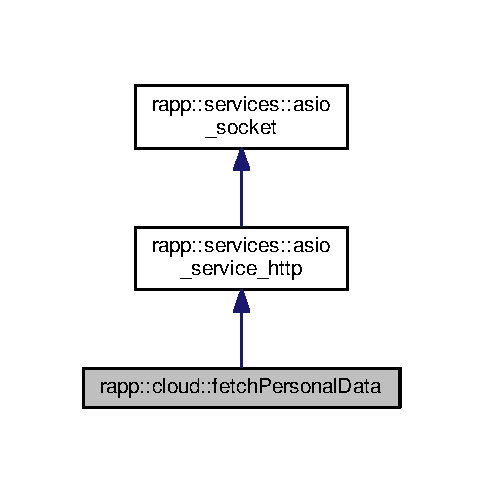
\includegraphics[width=232pt]{classrapp_1_1cloud_1_1fetchPersonalData__inherit__graph}
\end{center}
\end{figure}


Collaboration diagram for rapp\-:\-:cloud\-:\-:fetch\-Personal\-Data\-:
\nopagebreak
\begin{figure}[H]
\begin{center}
\leavevmode
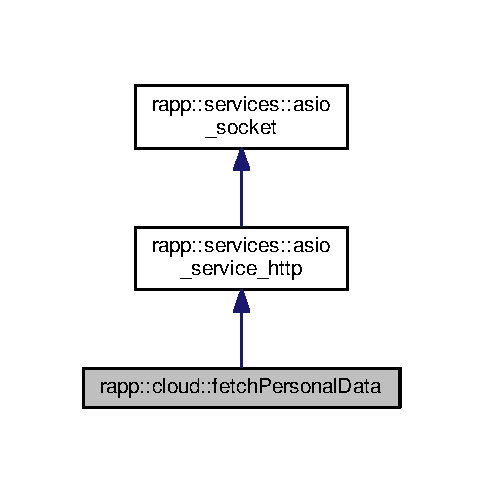
\includegraphics[width=232pt]{classrapp_1_1cloud_1_1fetchPersonalData__coll__graph}
\end{center}
\end{figure}
\subsection*{Public Member Functions}
\begin{DoxyCompactItemize}
\item 
\hyperlink{classrapp_1_1cloud_1_1fetchPersonalData_aeb9e23b12728550bc41683cded3174ad}{fetch\-Personal\-Data} (const std\-::string user, std\-::function$<$ void(const std\-::string) $>$ callback)
\begin{DoxyCompactList}\small\item\em Constructor for obtained personal (J\-S\-O\-N) data for a specific user. \end{DoxyCompactList}\end{DoxyCompactItemize}
\subsection*{Private Member Functions}
\begin{DoxyCompactItemize}
\item 
void \hyperlink{classrapp_1_1cloud_1_1fetchPersonalData_aa8df18d0cafd269ec4dcfbf5c4f44aa1}{handle\-\_\-reply} (std\-::string json)
\end{DoxyCompactItemize}
\subsection*{Private Attributes}
\begin{DoxyCompactItemize}
\item 
std\-::function$<$ void(const \\*
std\-::string) $>$ \hyperlink{classrapp_1_1cloud_1_1fetchPersonalData_a5ab89d0793a2d34182b13b4a4031e93d}{delegate\-\_\-\-\_\-}
\begin{DoxyCompactList}\small\item\em The callback called upon completion of receiving the detected faces. \end{DoxyCompactList}\end{DoxyCompactItemize}
\subsection*{Additional Inherited Members}


\subsection{Detailed Description}
Get all personal data for a specific user. 

\begin{DoxyVersion}{Version}
1 
\end{DoxyVersion}
\begin{DoxyDate}{Date}
18-\/\-April-\/2015 
\end{DoxyDate}
\begin{DoxyAuthor}{Author}
Alex Gkiokas \href{mailto:a.gkiokas@ortelio.co.uk}{\tt a.\-gkiokas@ortelio.\-co.\-uk} 
\end{DoxyAuthor}


Definition at line 14 of file fetch\-Personal\-Data.\-hpp.



\subsection{Constructor \& Destructor Documentation}
\hypertarget{classrapp_1_1cloud_1_1fetchPersonalData_aeb9e23b12728550bc41683cded3174ad}{\index{rapp\-::cloud\-::fetch\-Personal\-Data@{rapp\-::cloud\-::fetch\-Personal\-Data}!fetch\-Personal\-Data@{fetch\-Personal\-Data}}
\index{fetch\-Personal\-Data@{fetch\-Personal\-Data}!rapp::cloud::fetchPersonalData@{rapp\-::cloud\-::fetch\-Personal\-Data}}
\subsubsection[{fetch\-Personal\-Data}]{\setlength{\rightskip}{0pt plus 5cm}rapp\-::cloud\-::fetch\-Personal\-Data\-::fetch\-Personal\-Data (
\begin{DoxyParamCaption}
\item[{const std\-::string}]{user, }
\item[{std\-::function$<$ void(const std\-::string) $>$}]{callback}
\end{DoxyParamCaption}
)}}\label{classrapp_1_1cloud_1_1fetchPersonalData_aeb9e23b12728550bc41683cded3174ad}


Constructor for obtained personal (J\-S\-O\-N) data for a specific user. 


\begin{DoxyParams}{Parameters}
{\em user} & is the string username as stored in the database \\
\hline
{\em callback} & is the functor that will received the obtained data \\
\hline
\end{DoxyParams}
\begin{DoxyNote}{Note}
this is asynchronous, not serial, execution time may vary 
\end{DoxyNote}


Definition at line 24 of file fetch\-Personal\-Data.\-hpp.



\subsection{Member Function Documentation}
\hypertarget{classrapp_1_1cloud_1_1fetchPersonalData_aa8df18d0cafd269ec4dcfbf5c4f44aa1}{\index{rapp\-::cloud\-::fetch\-Personal\-Data@{rapp\-::cloud\-::fetch\-Personal\-Data}!handle\-\_\-reply@{handle\-\_\-reply}}
\index{handle\-\_\-reply@{handle\-\_\-reply}!rapp::cloud::fetchPersonalData@{rapp\-::cloud\-::fetch\-Personal\-Data}}
\subsubsection[{handle\-\_\-reply}]{\setlength{\rightskip}{0pt plus 5cm}void rapp\-::cloud\-::fetch\-Personal\-Data\-::handle\-\_\-reply (
\begin{DoxyParamCaption}
\item[{std\-::string}]{json}
\end{DoxyParamCaption}
)\hspace{0.3cm}{\ttfamily [private]}}}\label{classrapp_1_1cloud_1_1fetchPersonalData_aa8df18d0cafd269ec4dcfbf5c4f44aa1}
Get reply and send it directly to delegate \begin{DoxyNote}{Note}
we do not do any parsing at all here 
\end{DoxyNote}


Definition at line 51 of file fetch\-Personal\-Data.\-hpp.



\subsection{Member Data Documentation}
\hypertarget{classrapp_1_1cloud_1_1fetchPersonalData_a5ab89d0793a2d34182b13b4a4031e93d}{\index{rapp\-::cloud\-::fetch\-Personal\-Data@{rapp\-::cloud\-::fetch\-Personal\-Data}!delegate\-\_\-\-\_\-@{delegate\-\_\-\-\_\-}}
\index{delegate\-\_\-\-\_\-@{delegate\-\_\-\-\_\-}!rapp::cloud::fetchPersonalData@{rapp\-::cloud\-::fetch\-Personal\-Data}}
\subsubsection[{delegate\-\_\-\-\_\-}]{\setlength{\rightskip}{0pt plus 5cm}std\-::function$<$ void( const std\-::string ) $>$ rapp\-::cloud\-::fetch\-Personal\-Data\-::delegate\-\_\-\-\_\-\hspace{0.3cm}{\ttfamily [private]}}}\label{classrapp_1_1cloud_1_1fetchPersonalData_a5ab89d0793a2d34182b13b4a4031e93d}


The callback called upon completion of receiving the detected faces. 



Definition at line 57 of file fetch\-Personal\-Data.\-hpp.



The documentation for this class was generated from the following file\-:\begin{DoxyCompactItemize}
\item 
/home/travis/rapp\-\_\-temp/rapp-\/api/cpp/includes/cloud/fetch\-Personal\-Data/\hyperlink{fetchPersonalData_8hpp}{fetch\-Personal\-Data.\-hpp}\end{DoxyCompactItemize}

\hypertarget{classrapp_1_1robot_1_1nao}{\section{rapp\-:\-:robot\-:\-:nao Class Reference}
\label{classrapp_1_1robot_1_1nao}\index{rapp\-::robot\-::nao@{rapp\-::robot\-::nao}}
}


Implementation Class for Aldearan's N\-A\-O robot.  




{\ttfamily \#include $<$nao.\-hpp$>$}



Inheritance diagram for rapp\-:\-:robot\-:\-:nao\-:
\nopagebreak
\begin{figure}[H]
\begin{center}
\leavevmode
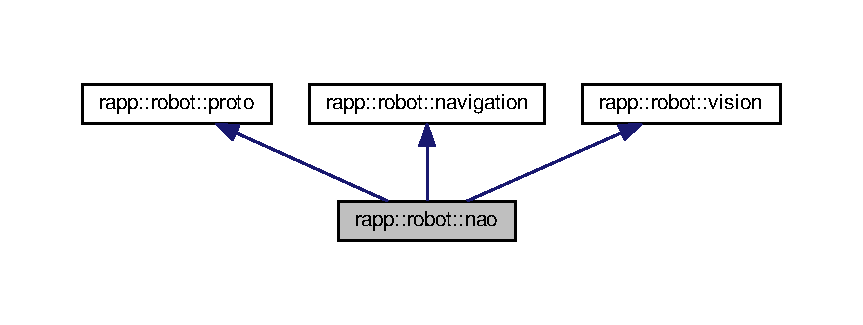
\includegraphics[width=350pt]{classrapp_1_1robot_1_1nao__inherit__graph}
\end{center}
\end{figure}


Collaboration diagram for rapp\-:\-:robot\-:\-:nao\-:
\nopagebreak
\begin{figure}[H]
\begin{center}
\leavevmode
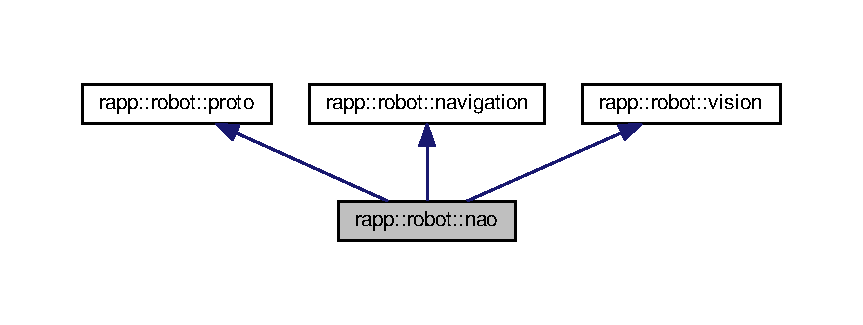
\includegraphics[width=350pt]{classrapp_1_1robot_1_1nao__coll__graph}
\end{center}
\end{figure}
\subsection*{Public Member Functions}
\begin{DoxyCompactItemize}
\item 
\hyperlink{classrapp_1_1robot_1_1nao_a00956d04e6061d875e0352c360e4d8a6}{nao} ()=default
\begin{DoxyCompactList}\small\item\em Constructor ? \end{DoxyCompactList}\item 
std\-::shared\-\_\-pointr\\*
$<$ \hyperlink{classrapp_1_1object_1_1picture}{rapp\-::object\-::picture} $>$ \hyperlink{classrapp_1_1robot_1_1nao_a276172d720ce8387a3fe695e02753af0}{capture\-Image} (std\-::string camera\-Id, int camera\-Resolution) const 
\begin{DoxyCompactList}\small\item\em N\-O\-T\-E\-: What about format? \end{DoxyCompactList}\item 
void move \hyperlink{classrapp_1_1robot_1_1nao_a4b99876e6fa503830cd1a8c93267eb9f}{Head} (float yaw, float pitch)
\item 
void \hyperlink{classrapp_1_1robot_1_1nao_a8a3d202cdc642ffcc0d6678a0b3b62c5}{look\-At\-Point} (float x, float y, float z)
\item 
std\-::string \hyperlink{classrapp_1_1robot_1_1nao_aed3ffea92e69e9e0fba684c42f5f7cfd}{model} () const 
\begin{DoxyCompactList}\small\item\em Get Robot's Model. \end{DoxyCompactList}\item 
void \hyperlink{classrapp_1_1robot_1_1nao_a313e2ddb5b0d08e96bf79b29542f0b40}{move\-Joint} (std\-::string joint, float angle)
\item 
void \hyperlink{classrapp_1_1robot_1_1nao_a50e3841d836ccaa74852c083297beb7b}{move\-Stop} ()
\item 
void \hyperlink{classrapp_1_1robot_1_1nao_a7404089508af1b7a2872a29990fc6dc2}{move\-To} (float x, float y, float z)
\begin{DoxyCompactList}\small\item\em T\-O\-D\-O\-: Describe each parameter and explain what it is. \end{DoxyCompactList}\item 
void \hyperlink{classrapp_1_1robot_1_1nao_a8b2a03a5e46e86d0aedb1d239ffcdcf9}{move\-Vel} (float x, float y, float z)
\item 
void \hyperlink{classrapp_1_1robot_1_1nao_a707430d6f61a7eb24a020498d9fef841}{remove\-Stiffness} (std\-::string joint)
\item 
std\-::string \hyperlink{classrapp_1_1robot_1_1nao_a0eb438d37b7958554ba43b7b3cddf131}{ruid} () const 
\begin{DoxyCompactList}\small\item\em Get Robot's Unique I\-D. \end{DoxyCompactList}\item 
void \hyperlink{classrapp_1_1robot_1_1nao_a96e6289bc1c1782a79ba0ca4d82fb828}{take\-Predefined\-Posture} (std\-::string pose)
\item 
void \hyperlink{classrapp_1_1robot_1_1nao_a8810ac769c75fa2f4723770c9e58a17e}{vis\-Odom} ()
\end{DoxyCompactItemize}


\subsection{Detailed Description}
Implementation Class for Aldearan's N\-A\-O robot. 

\begin{DoxyVersion}{Version}
1 
\end{DoxyVersion}
\begin{DoxyDate}{Date}
20-\/\-September-\/2015 
\end{DoxyDate}
\begin{DoxyAuthor}{Author}
Alex Gkiokas \href{mailto:a.gkiokas@ortelio.co.uk}{\tt a.\-gkiokas@ortelio.\-co.\-uk} 
\end{DoxyAuthor}


Definition at line 13 of file nao.\-hpp.



\subsection{Constructor \& Destructor Documentation}
\hypertarget{classrapp_1_1robot_1_1nao_a00956d04e6061d875e0352c360e4d8a6}{\index{rapp\-::robot\-::nao@{rapp\-::robot\-::nao}!nao@{nao}}
\index{nao@{nao}!rapp::robot::nao@{rapp\-::robot\-::nao}}
\subsubsection[{nao}]{\setlength{\rightskip}{0pt plus 5cm}rapp\-::robot\-::nao\-::nao (
\begin{DoxyParamCaption}
{}
\end{DoxyParamCaption}
)\hspace{0.3cm}{\ttfamily [default]}}}\label{classrapp_1_1robot_1_1nao_a00956d04e6061d875e0352c360e4d8a6}


Constructor ? 



\subsection{Member Function Documentation}
\hypertarget{classrapp_1_1robot_1_1nao_a276172d720ce8387a3fe695e02753af0}{\index{rapp\-::robot\-::nao@{rapp\-::robot\-::nao}!capture\-Image@{capture\-Image}}
\index{capture\-Image@{capture\-Image}!rapp::robot::nao@{rapp\-::robot\-::nao}}
\subsubsection[{capture\-Image}]{\setlength{\rightskip}{0pt plus 5cm}std\-::shared\-\_\-pointr$<${\bf rapp\-::object\-::picture}$>$ rapp\-::robot\-::nao\-::capture\-Image (
\begin{DoxyParamCaption}
\item[{std\-::string}]{camera\-Id, }
\item[{int}]{camera\-Resolution}
\end{DoxyParamCaption}
) const\hspace{0.3cm}{\ttfamily [virtual]}}}\label{classrapp_1_1robot_1_1nao_a276172d720ce8387a3fe695e02753af0}


N\-O\-T\-E\-: What about format? 



Implements \hyperlink{classrapp_1_1robot_1_1vision_ac6f224f2da0d9512b8c6700de3eded85}{rapp\-::robot\-::vision}.

\hypertarget{classrapp_1_1robot_1_1nao_a4b99876e6fa503830cd1a8c93267eb9f}{\index{rapp\-::robot\-::nao@{rapp\-::robot\-::nao}!Head@{Head}}
\index{Head@{Head}!rapp::robot::nao@{rapp\-::robot\-::nao}}
\subsubsection[{Head}]{\setlength{\rightskip}{0pt plus 5cm}void move rapp\-::robot\-::nao\-::\-Head (
\begin{DoxyParamCaption}
\item[{float}]{yaw, }
\item[{float}]{pitch}
\end{DoxyParamCaption}
)}}\label{classrapp_1_1robot_1_1nao_a4b99876e6fa503830cd1a8c93267eb9f}
\hypertarget{classrapp_1_1robot_1_1nao_a8a3d202cdc642ffcc0d6678a0b3b62c5}{\index{rapp\-::robot\-::nao@{rapp\-::robot\-::nao}!look\-At\-Point@{look\-At\-Point}}
\index{look\-At\-Point@{look\-At\-Point}!rapp::robot::nao@{rapp\-::robot\-::nao}}
\subsubsection[{look\-At\-Point}]{\setlength{\rightskip}{0pt plus 5cm}void rapp\-::robot\-::nao\-::look\-At\-Point (
\begin{DoxyParamCaption}
\item[{float}]{x, }
\item[{float}]{y, }
\item[{float}]{z}
\end{DoxyParamCaption}
)\hspace{0.3cm}{\ttfamily [virtual]}}}\label{classrapp_1_1robot_1_1nao_a8a3d202cdc642ffcc0d6678a0b3b62c5}


Implements \hyperlink{classrapp_1_1robot_1_1navigation_a3b9fa18bda273730de4439f324c1bcfb}{rapp\-::robot\-::navigation}.

\hypertarget{classrapp_1_1robot_1_1nao_aed3ffea92e69e9e0fba684c42f5f7cfd}{\index{rapp\-::robot\-::nao@{rapp\-::robot\-::nao}!model@{model}}
\index{model@{model}!rapp::robot::nao@{rapp\-::robot\-::nao}}
\subsubsection[{model}]{\setlength{\rightskip}{0pt plus 5cm}std\-::string rapp\-::robot\-::nao\-::model (
\begin{DoxyParamCaption}
{}
\end{DoxyParamCaption}
) const\hspace{0.3cm}{\ttfamily [virtual]}}}\label{classrapp_1_1robot_1_1nao_aed3ffea92e69e9e0fba684c42f5f7cfd}


Get Robot's Model. 



Implements \hyperlink{classrapp_1_1robot_1_1proto_ace501b12c79698041f37a90306163aa9}{rapp\-::robot\-::proto}.

\hypertarget{classrapp_1_1robot_1_1nao_a313e2ddb5b0d08e96bf79b29542f0b40}{\index{rapp\-::robot\-::nao@{rapp\-::robot\-::nao}!move\-Joint@{move\-Joint}}
\index{move\-Joint@{move\-Joint}!rapp::robot::nao@{rapp\-::robot\-::nao}}
\subsubsection[{move\-Joint}]{\setlength{\rightskip}{0pt plus 5cm}void rapp\-::robot\-::nao\-::move\-Joint (
\begin{DoxyParamCaption}
\item[{std\-::string}]{joint, }
\item[{float}]{angle}
\end{DoxyParamCaption}
)\hspace{0.3cm}{\ttfamily [virtual]}}}\label{classrapp_1_1robot_1_1nao_a313e2ddb5b0d08e96bf79b29542f0b40}


Implements \hyperlink{classrapp_1_1robot_1_1navigation_ae23002930f3df05efea1db90b7ede477}{rapp\-::robot\-::navigation}.

\hypertarget{classrapp_1_1robot_1_1nao_a50e3841d836ccaa74852c083297beb7b}{\index{rapp\-::robot\-::nao@{rapp\-::robot\-::nao}!move\-Stop@{move\-Stop}}
\index{move\-Stop@{move\-Stop}!rapp::robot::nao@{rapp\-::robot\-::nao}}
\subsubsection[{move\-Stop}]{\setlength{\rightskip}{0pt plus 5cm}void rapp\-::robot\-::nao\-::move\-Stop (
\begin{DoxyParamCaption}
{}
\end{DoxyParamCaption}
)\hspace{0.3cm}{\ttfamily [virtual]}}}\label{classrapp_1_1robot_1_1nao_a50e3841d836ccaa74852c083297beb7b}


Implements \hyperlink{classrapp_1_1robot_1_1navigation_a1ed5e2e425e54f18ff1708ff4f91423e}{rapp\-::robot\-::navigation}.

\hypertarget{classrapp_1_1robot_1_1nao_a7404089508af1b7a2872a29990fc6dc2}{\index{rapp\-::robot\-::nao@{rapp\-::robot\-::nao}!move\-To@{move\-To}}
\index{move\-To@{move\-To}!rapp::robot::nao@{rapp\-::robot\-::nao}}
\subsubsection[{move\-To}]{\setlength{\rightskip}{0pt plus 5cm}void rapp\-::robot\-::nao\-::move\-To (
\begin{DoxyParamCaption}
\item[{float}]{x, }
\item[{float}]{y, }
\item[{float}]{theta}
\end{DoxyParamCaption}
)\hspace{0.3cm}{\ttfamily [virtual]}}}\label{classrapp_1_1robot_1_1nao_a7404089508af1b7a2872a29990fc6dc2}


T\-O\-D\-O\-: Describe each parameter and explain what it is. 



Implements \hyperlink{classrapp_1_1robot_1_1navigation_ab9015aedc583ec4a86cf3c4a28a9eede}{rapp\-::robot\-::navigation}.

\hypertarget{classrapp_1_1robot_1_1nao_a8b2a03a5e46e86d0aedb1d239ffcdcf9}{\index{rapp\-::robot\-::nao@{rapp\-::robot\-::nao}!move\-Vel@{move\-Vel}}
\index{move\-Vel@{move\-Vel}!rapp::robot::nao@{rapp\-::robot\-::nao}}
\subsubsection[{move\-Vel}]{\setlength{\rightskip}{0pt plus 5cm}void rapp\-::robot\-::nao\-::move\-Vel (
\begin{DoxyParamCaption}
\item[{float}]{x, }
\item[{float}]{y, }
\item[{float}]{z}
\end{DoxyParamCaption}
)\hspace{0.3cm}{\ttfamily [virtual]}}}\label{classrapp_1_1robot_1_1nao_a8b2a03a5e46e86d0aedb1d239ffcdcf9}


Implements \hyperlink{classrapp_1_1robot_1_1navigation_ad9edf8af6a0ed5660c4ff1cb93752f3d}{rapp\-::robot\-::navigation}.

\hypertarget{classrapp_1_1robot_1_1nao_a707430d6f61a7eb24a020498d9fef841}{\index{rapp\-::robot\-::nao@{rapp\-::robot\-::nao}!remove\-Stiffness@{remove\-Stiffness}}
\index{remove\-Stiffness@{remove\-Stiffness}!rapp::robot::nao@{rapp\-::robot\-::nao}}
\subsubsection[{remove\-Stiffness}]{\setlength{\rightskip}{0pt plus 5cm}void rapp\-::robot\-::nao\-::remove\-Stiffness (
\begin{DoxyParamCaption}
\item[{std\-::string}]{joint}
\end{DoxyParamCaption}
)}}\label{classrapp_1_1robot_1_1nao_a707430d6f61a7eb24a020498d9fef841}
\hypertarget{classrapp_1_1robot_1_1nao_a0eb438d37b7958554ba43b7b3cddf131}{\index{rapp\-::robot\-::nao@{rapp\-::robot\-::nao}!ruid@{ruid}}
\index{ruid@{ruid}!rapp::robot::nao@{rapp\-::robot\-::nao}}
\subsubsection[{ruid}]{\setlength{\rightskip}{0pt plus 5cm}std\-::string rapp\-::robot\-::nao\-::ruid (
\begin{DoxyParamCaption}
{}
\end{DoxyParamCaption}
) const\hspace{0.3cm}{\ttfamily [virtual]}}}\label{classrapp_1_1robot_1_1nao_a0eb438d37b7958554ba43b7b3cddf131}


Get Robot's Unique I\-D. 



Implements \hyperlink{classrapp_1_1robot_1_1proto_a2d0dd7d28350e8a7c6ffb7616c0a6f5f}{rapp\-::robot\-::proto}.

\hypertarget{classrapp_1_1robot_1_1nao_a96e6289bc1c1782a79ba0ca4d82fb828}{\index{rapp\-::robot\-::nao@{rapp\-::robot\-::nao}!take\-Predefined\-Posture@{take\-Predefined\-Posture}}
\index{take\-Predefined\-Posture@{take\-Predefined\-Posture}!rapp::robot::nao@{rapp\-::robot\-::nao}}
\subsubsection[{take\-Predefined\-Posture}]{\setlength{\rightskip}{0pt plus 5cm}void rapp\-::robot\-::nao\-::take\-Predefined\-Posture (
\begin{DoxyParamCaption}
\item[{std\-::string}]{pose}
\end{DoxyParamCaption}
)\hspace{0.3cm}{\ttfamily [virtual]}}}\label{classrapp_1_1robot_1_1nao_a96e6289bc1c1782a79ba0ca4d82fb828}
N\-O\-T\-E\-: parameter pose could be a class of its own, because it encapsulates some kind of Robot State. 

Implements \hyperlink{classrapp_1_1robot_1_1navigation_a135033e445d05cc3e50c3942d47e296e}{rapp\-::robot\-::navigation}.

\hypertarget{classrapp_1_1robot_1_1nao_a8810ac769c75fa2f4723770c9e58a17e}{\index{rapp\-::robot\-::nao@{rapp\-::robot\-::nao}!vis\-Odom@{vis\-Odom}}
\index{vis\-Odom@{vis\-Odom}!rapp::robot::nao@{rapp\-::robot\-::nao}}
\subsubsection[{vis\-Odom}]{\setlength{\rightskip}{0pt plus 5cm}void rapp\-::robot\-::nao\-::vis\-Odom (
\begin{DoxyParamCaption}
{}
\end{DoxyParamCaption}
)\hspace{0.3cm}{\ttfamily [virtual]}}}\label{classrapp_1_1robot_1_1nao_a8810ac769c75fa2f4723770c9e58a17e}


Implements \hyperlink{classrapp_1_1robot_1_1navigation_aefd121347fad3dabed99dae344067ca4}{rapp\-::robot\-::navigation}.



The documentation for this class was generated from the following file\-:\begin{DoxyCompactItemize}
\item 
/home/travis/rapp\-\_\-temp/rapp-\/api/cpp/includes/robot/nao/\hyperlink{nao_8hpp}{nao.\-hpp}\end{DoxyCompactItemize}

\hypertarget{classrapp_1_1robot_1_1navigation}{\section{rapp\-:\-:robot\-:\-:navigation Class Reference}
\label{classrapp_1_1robot_1_1navigation}\index{rapp\-::robot\-::navigation@{rapp\-::robot\-::navigation}}
}


Abstract Base Class (A\-B\-C) Interface for Navigation.  




{\ttfamily \#include $<$navigation.\-hpp$>$}



Inheritance diagram for rapp\-:\-:robot\-:\-:navigation\-:
\nopagebreak
\begin{figure}[H]
\begin{center}
\leavevmode
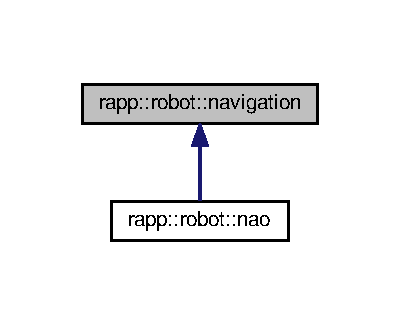
\includegraphics[width=192pt]{classrapp_1_1robot_1_1navigation__inherit__graph}
\end{center}
\end{figure}
\subsection*{Public Member Functions}
\begin{DoxyCompactItemize}
\item 
virtual void \hyperlink{classrapp_1_1robot_1_1navigation_a3b9fa18bda273730de4439f324c1bcfb}{look\-At\-Point} (float x, float y, float z)=0
\item 
virtual void \hyperlink{classrapp_1_1robot_1_1navigation_afb8024b5245696ea13c2143912fe1bb2}{move\-Head} (float yaw, float pitch)=0
\item 
virtual void \hyperlink{classrapp_1_1robot_1_1navigation_ae23002930f3df05efea1db90b7ede477}{move\-Joint} (std\-::string joint, float angle)=0
\item 
virtual void \hyperlink{classrapp_1_1robot_1_1navigation_a1ed5e2e425e54f18ff1708ff4f91423e}{move\-Stop} ()=0
\item 
virtual void \hyperlink{classrapp_1_1robot_1_1navigation_ab9015aedc583ec4a86cf3c4a28a9eede}{move\-To} (float x, float y, float theta)=0
\begin{DoxyCompactList}\small\item\em T\-O\-D\-O\-: Describe each parameter and explain what it is. \end{DoxyCompactList}\item 
virtual void \hyperlink{classrapp_1_1robot_1_1navigation_ad9edf8af6a0ed5660c4ff1cb93752f3d}{move\-Vel} (float x, float y, float theta)=0
\item 
virtual void \hyperlink{classrapp_1_1robot_1_1navigation_ae8585c277d4e0f967f4a3a5555ca15d4}{remove\-Stiffness} (std\-::string joint) const =0
\item 
virtual void \hyperlink{classrapp_1_1robot_1_1navigation_a135033e445d05cc3e50c3942d47e296e}{take\-Predefined\-Posture} (std\-::string pose)=0
\item 
virtual void \hyperlink{classrapp_1_1robot_1_1navigation_aefd121347fad3dabed99dae344067ca4}{vis\-Odom} ()=0
\end{DoxyCompactItemize}


\subsection{Detailed Description}
Abstract Base Class (A\-B\-C) Interface for Navigation. 

\begin{DoxyVersion}{Version}
1 
\end{DoxyVersion}
\begin{DoxyDate}{Date}
20-\/\-September-\/2015 
\end{DoxyDate}
\begin{DoxyAuthor}{Author}
Alex Gkiokas \href{mailto:a.gkiokas@ortelio.co.uk}{\tt a.\-gkiokas@ortelio.\-co.\-uk} 
\end{DoxyAuthor}


Definition at line 13 of file navigation.\-hpp.



\subsection{Member Function Documentation}
\hypertarget{classrapp_1_1robot_1_1navigation_a3b9fa18bda273730de4439f324c1bcfb}{\index{rapp\-::robot\-::navigation@{rapp\-::robot\-::navigation}!look\-At\-Point@{look\-At\-Point}}
\index{look\-At\-Point@{look\-At\-Point}!rapp::robot::navigation@{rapp\-::robot\-::navigation}}
\subsubsection[{look\-At\-Point}]{\setlength{\rightskip}{0pt plus 5cm}virtual void rapp\-::robot\-::navigation\-::look\-At\-Point (
\begin{DoxyParamCaption}
\item[{float}]{x, }
\item[{float}]{y, }
\item[{float}]{z}
\end{DoxyParamCaption}
)\hspace{0.3cm}{\ttfamily [pure virtual]}}}\label{classrapp_1_1robot_1_1navigation_a3b9fa18bda273730de4439f324c1bcfb}


Implemented in \hyperlink{classrapp_1_1robot_1_1nao_a8a3d202cdc642ffcc0d6678a0b3b62c5}{rapp\-::robot\-::nao}.

\hypertarget{classrapp_1_1robot_1_1navigation_afb8024b5245696ea13c2143912fe1bb2}{\index{rapp\-::robot\-::navigation@{rapp\-::robot\-::navigation}!move\-Head@{move\-Head}}
\index{move\-Head@{move\-Head}!rapp::robot::navigation@{rapp\-::robot\-::navigation}}
\subsubsection[{move\-Head}]{\setlength{\rightskip}{0pt plus 5cm}virtual void rapp\-::robot\-::navigation\-::move\-Head (
\begin{DoxyParamCaption}
\item[{float}]{yaw, }
\item[{float}]{pitch}
\end{DoxyParamCaption}
)\hspace{0.3cm}{\ttfamily [pure virtual]}}}\label{classrapp_1_1robot_1_1navigation_afb8024b5245696ea13c2143912fe1bb2}
\hypertarget{classrapp_1_1robot_1_1navigation_ae23002930f3df05efea1db90b7ede477}{\index{rapp\-::robot\-::navigation@{rapp\-::robot\-::navigation}!move\-Joint@{move\-Joint}}
\index{move\-Joint@{move\-Joint}!rapp::robot::navigation@{rapp\-::robot\-::navigation}}
\subsubsection[{move\-Joint}]{\setlength{\rightskip}{0pt plus 5cm}virtual void rapp\-::robot\-::navigation\-::move\-Joint (
\begin{DoxyParamCaption}
\item[{std\-::string}]{joint, }
\item[{float}]{angle}
\end{DoxyParamCaption}
)\hspace{0.3cm}{\ttfamily [pure virtual]}}}\label{classrapp_1_1robot_1_1navigation_ae23002930f3df05efea1db90b7ede477}


Implemented in \hyperlink{classrapp_1_1robot_1_1nao_a313e2ddb5b0d08e96bf79b29542f0b40}{rapp\-::robot\-::nao}.

\hypertarget{classrapp_1_1robot_1_1navigation_a1ed5e2e425e54f18ff1708ff4f91423e}{\index{rapp\-::robot\-::navigation@{rapp\-::robot\-::navigation}!move\-Stop@{move\-Stop}}
\index{move\-Stop@{move\-Stop}!rapp::robot::navigation@{rapp\-::robot\-::navigation}}
\subsubsection[{move\-Stop}]{\setlength{\rightskip}{0pt plus 5cm}virtual void rapp\-::robot\-::navigation\-::move\-Stop (
\begin{DoxyParamCaption}
{}
\end{DoxyParamCaption}
)\hspace{0.3cm}{\ttfamily [pure virtual]}}}\label{classrapp_1_1robot_1_1navigation_a1ed5e2e425e54f18ff1708ff4f91423e}


Implemented in \hyperlink{classrapp_1_1robot_1_1nao_a50e3841d836ccaa74852c083297beb7b}{rapp\-::robot\-::nao}.

\hypertarget{classrapp_1_1robot_1_1navigation_ab9015aedc583ec4a86cf3c4a28a9eede}{\index{rapp\-::robot\-::navigation@{rapp\-::robot\-::navigation}!move\-To@{move\-To}}
\index{move\-To@{move\-To}!rapp::robot::navigation@{rapp\-::robot\-::navigation}}
\subsubsection[{move\-To}]{\setlength{\rightskip}{0pt plus 5cm}virtual void rapp\-::robot\-::navigation\-::move\-To (
\begin{DoxyParamCaption}
\item[{float}]{x, }
\item[{float}]{y, }
\item[{float}]{theta}
\end{DoxyParamCaption}
)\hspace{0.3cm}{\ttfamily [pure virtual]}}}\label{classrapp_1_1robot_1_1navigation_ab9015aedc583ec4a86cf3c4a28a9eede}


T\-O\-D\-O\-: Describe each parameter and explain what it is. 



Implemented in \hyperlink{classrapp_1_1robot_1_1nao_a7404089508af1b7a2872a29990fc6dc2}{rapp\-::robot\-::nao}.

\hypertarget{classrapp_1_1robot_1_1navigation_ad9edf8af6a0ed5660c4ff1cb93752f3d}{\index{rapp\-::robot\-::navigation@{rapp\-::robot\-::navigation}!move\-Vel@{move\-Vel}}
\index{move\-Vel@{move\-Vel}!rapp::robot::navigation@{rapp\-::robot\-::navigation}}
\subsubsection[{move\-Vel}]{\setlength{\rightskip}{0pt plus 5cm}virtual void rapp\-::robot\-::navigation\-::move\-Vel (
\begin{DoxyParamCaption}
\item[{float}]{x, }
\item[{float}]{y, }
\item[{float}]{theta}
\end{DoxyParamCaption}
)\hspace{0.3cm}{\ttfamily [pure virtual]}}}\label{classrapp_1_1robot_1_1navigation_ad9edf8af6a0ed5660c4ff1cb93752f3d}


Implemented in \hyperlink{classrapp_1_1robot_1_1nao_a8b2a03a5e46e86d0aedb1d239ffcdcf9}{rapp\-::robot\-::nao}.

\hypertarget{classrapp_1_1robot_1_1navigation_ae8585c277d4e0f967f4a3a5555ca15d4}{\index{rapp\-::robot\-::navigation@{rapp\-::robot\-::navigation}!remove\-Stiffness@{remove\-Stiffness}}
\index{remove\-Stiffness@{remove\-Stiffness}!rapp::robot::navigation@{rapp\-::robot\-::navigation}}
\subsubsection[{remove\-Stiffness}]{\setlength{\rightskip}{0pt plus 5cm}virtual void rapp\-::robot\-::navigation\-::remove\-Stiffness (
\begin{DoxyParamCaption}
\item[{std\-::string}]{joint}
\end{DoxyParamCaption}
) const\hspace{0.3cm}{\ttfamily [pure virtual]}}}\label{classrapp_1_1robot_1_1navigation_ae8585c277d4e0f967f4a3a5555ca15d4}
\hypertarget{classrapp_1_1robot_1_1navigation_a135033e445d05cc3e50c3942d47e296e}{\index{rapp\-::robot\-::navigation@{rapp\-::robot\-::navigation}!take\-Predefined\-Posture@{take\-Predefined\-Posture}}
\index{take\-Predefined\-Posture@{take\-Predefined\-Posture}!rapp::robot::navigation@{rapp\-::robot\-::navigation}}
\subsubsection[{take\-Predefined\-Posture}]{\setlength{\rightskip}{0pt plus 5cm}virtual void rapp\-::robot\-::navigation\-::take\-Predefined\-Posture (
\begin{DoxyParamCaption}
\item[{std\-::string}]{pose}
\end{DoxyParamCaption}
)\hspace{0.3cm}{\ttfamily [pure virtual]}}}\label{classrapp_1_1robot_1_1navigation_a135033e445d05cc3e50c3942d47e296e}
N\-O\-T\-E\-: parameter pose could be a class of its own, because it encapsulates some kind of Robot State. 

Implemented in \hyperlink{classrapp_1_1robot_1_1nao_a96e6289bc1c1782a79ba0ca4d82fb828}{rapp\-::robot\-::nao}.

\hypertarget{classrapp_1_1robot_1_1navigation_aefd121347fad3dabed99dae344067ca4}{\index{rapp\-::robot\-::navigation@{rapp\-::robot\-::navigation}!vis\-Odom@{vis\-Odom}}
\index{vis\-Odom@{vis\-Odom}!rapp::robot::navigation@{rapp\-::robot\-::navigation}}
\subsubsection[{vis\-Odom}]{\setlength{\rightskip}{0pt plus 5cm}virtual void rapp\-::robot\-::navigation\-::vis\-Odom (
\begin{DoxyParamCaption}
{}
\end{DoxyParamCaption}
)\hspace{0.3cm}{\ttfamily [pure virtual]}}}\label{classrapp_1_1robot_1_1navigation_aefd121347fad3dabed99dae344067ca4}


Implemented in \hyperlink{classrapp_1_1robot_1_1nao_a8810ac769c75fa2f4723770c9e58a17e}{rapp\-::robot\-::nao}.



The documentation for this class was generated from the following file\-:\begin{DoxyCompactItemize}
\item 
/home/travis/rapp\-\_\-temp/rapp-\/api/cpp/includes/robot/navigation/\hyperlink{navigation_8hpp}{navigation.\-hpp}\end{DoxyCompactItemize}

\hypertarget{classrapp_1_1cloud_1_1ontologyIsSubSuperClassOf}{\section{rapp\-:\-:cloud\-:\-:ontology\-Is\-Sub\-Super\-Class\-Of Class Reference}
\label{classrapp_1_1cloud_1_1ontologyIsSubSuperClassOf}\index{rapp\-::cloud\-::ontology\-Is\-Sub\-Super\-Class\-Of@{rapp\-::cloud\-::ontology\-Is\-Sub\-Super\-Class\-Of}}
}


{\ttfamily \#include $<$ontology\-Is\-Sub\-Super\-Class\-Of.\-hpp$>$}



Inheritance diagram for rapp\-:\-:cloud\-:\-:ontology\-Is\-Sub\-Super\-Class\-Of\-:
\nopagebreak
\begin{figure}[H]
\begin{center}
\leavevmode
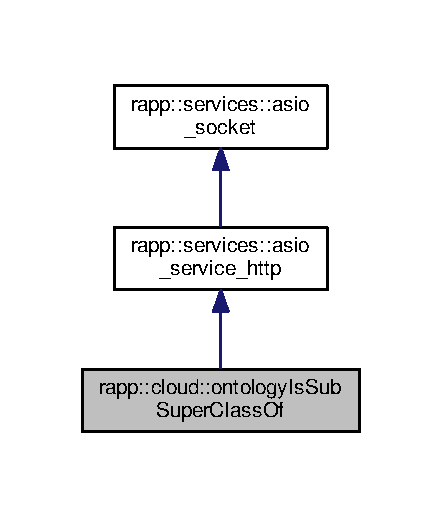
\includegraphics[width=212pt]{classrapp_1_1cloud_1_1ontologyIsSubSuperClassOf__inherit__graph}
\end{center}
\end{figure}


Collaboration diagram for rapp\-:\-:cloud\-:\-:ontology\-Is\-Sub\-Super\-Class\-Of\-:
\nopagebreak
\begin{figure}[H]
\begin{center}
\leavevmode
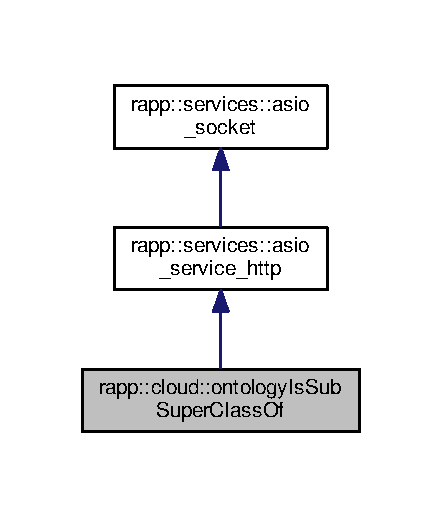
\includegraphics[width=212pt]{classrapp_1_1cloud_1_1ontologyIsSubSuperClassOf__coll__graph}
\end{center}
\end{figure}
\subsection*{Public Member Functions}
\begin{DoxyCompactItemize}
\item 
\hyperlink{classrapp_1_1cloud_1_1ontologyIsSubSuperClassOf_ae498a2ccfc4db700c39b163b73870d72}{ontology\-Is\-Sub\-Super\-Class\-Of} (const std\-::string parent, const std\-::string child, bool recursive, std\-::function$<$ void(bool result) $>$ callback)
\begin{DoxyCompactList}\small\item\em Constructor for this handler. \end{DoxyCompactList}\end{DoxyCompactItemize}
\subsection*{Private Member Functions}
\begin{DoxyCompactItemize}
\item 
void \hyperlink{classrapp_1_1cloud_1_1ontologyIsSubSuperClassOf_a579c9d44e2017b2a9db3ff938672645e}{handle\-\_\-reply} (std\-::string json)
\end{DoxyCompactItemize}
\subsection*{Private Attributes}
\begin{DoxyCompactItemize}
\item 
std\-::function$<$ void(bool result) $>$ \hyperlink{classrapp_1_1cloud_1_1ontologyIsSubSuperClassOf_a119bd48f23d64fc2f652cb53d2b21151}{delegate\-\_\-\-\_\-}
\begin{DoxyCompactList}\small\item\em The callback called upon completion of receiving the detected faces. \end{DoxyCompactList}\end{DoxyCompactItemize}
\subsection*{Additional Inherited Members}


\subsection{Detailed Description}


Definition at line 13 of file ontology\-Is\-Sub\-Super\-Class\-Of.\-hpp.



\subsection{Constructor \& Destructor Documentation}
\hypertarget{classrapp_1_1cloud_1_1ontologyIsSubSuperClassOf_ae498a2ccfc4db700c39b163b73870d72}{\index{rapp\-::cloud\-::ontology\-Is\-Sub\-Super\-Class\-Of@{rapp\-::cloud\-::ontology\-Is\-Sub\-Super\-Class\-Of}!ontology\-Is\-Sub\-Super\-Class\-Of@{ontology\-Is\-Sub\-Super\-Class\-Of}}
\index{ontology\-Is\-Sub\-Super\-Class\-Of@{ontology\-Is\-Sub\-Super\-Class\-Of}!rapp::cloud::ontologyIsSubSuperClassOf@{rapp\-::cloud\-::ontology\-Is\-Sub\-Super\-Class\-Of}}
\subsubsection[{ontology\-Is\-Sub\-Super\-Class\-Of}]{\setlength{\rightskip}{0pt plus 5cm}rapp\-::cloud\-::ontology\-Is\-Sub\-Super\-Class\-Of\-::ontology\-Is\-Sub\-Super\-Class\-Of (
\begin{DoxyParamCaption}
\item[{const std\-::string}]{parent, }
\item[{const std\-::string}]{child, }
\item[{bool}]{recursive, }
\item[{std\-::function$<$ void(bool result) $>$}]{callback}
\end{DoxyParamCaption}
)}}\label{classrapp_1_1cloud_1_1ontologyIsSubSuperClassOf_ae498a2ccfc4db700c39b163b73870d72}


Constructor for this handler. 


\begin{DoxyParams}{Parameters}
{\em query} & is the entity for which we will try to acquire its ? \\
\hline
{\em callback} & is the functor that will receive the classes discovered \\
\hline
\end{DoxyParams}


Definition at line 22 of file ontology\-Is\-Sub\-Super\-Class\-Of.\-hpp.



\subsection{Member Function Documentation}
\hypertarget{classrapp_1_1cloud_1_1ontologyIsSubSuperClassOf_a579c9d44e2017b2a9db3ff938672645e}{\index{rapp\-::cloud\-::ontology\-Is\-Sub\-Super\-Class\-Of@{rapp\-::cloud\-::ontology\-Is\-Sub\-Super\-Class\-Of}!handle\-\_\-reply@{handle\-\_\-reply}}
\index{handle\-\_\-reply@{handle\-\_\-reply}!rapp::cloud::ontologyIsSubSuperClassOf@{rapp\-::cloud\-::ontology\-Is\-Sub\-Super\-Class\-Of}}
\subsubsection[{handle\-\_\-reply}]{\setlength{\rightskip}{0pt plus 5cm}void rapp\-::cloud\-::ontology\-Is\-Sub\-Super\-Class\-Of\-::handle\-\_\-reply (
\begin{DoxyParamCaption}
\item[{std\-::string}]{json}
\end{DoxyParamCaption}
)\hspace{0.3cm}{\ttfamily [private]}}}\label{classrapp_1_1cloud_1_1ontologyIsSubSuperClassOf_a579c9d44e2017b2a9db3ff938672645e}


Definition at line 43 of file ontology\-Is\-Sub\-Super\-Class\-Of.\-hpp.



\subsection{Member Data Documentation}
\hypertarget{classrapp_1_1cloud_1_1ontologyIsSubSuperClassOf_a119bd48f23d64fc2f652cb53d2b21151}{\index{rapp\-::cloud\-::ontology\-Is\-Sub\-Super\-Class\-Of@{rapp\-::cloud\-::ontology\-Is\-Sub\-Super\-Class\-Of}!delegate\-\_\-\-\_\-@{delegate\-\_\-\-\_\-}}
\index{delegate\-\_\-\-\_\-@{delegate\-\_\-\-\_\-}!rapp::cloud::ontologyIsSubSuperClassOf@{rapp\-::cloud\-::ontology\-Is\-Sub\-Super\-Class\-Of}}
\subsubsection[{delegate\-\_\-\-\_\-}]{\setlength{\rightskip}{0pt plus 5cm}std\-::function$<$ void( bool result ) $>$ rapp\-::cloud\-::ontology\-Is\-Sub\-Super\-Class\-Of\-::delegate\-\_\-\-\_\-\hspace{0.3cm}{\ttfamily [private]}}}\label{classrapp_1_1cloud_1_1ontologyIsSubSuperClassOf_a119bd48f23d64fc2f652cb53d2b21151}


The callback called upon completion of receiving the detected faces. 



Definition at line 77 of file ontology\-Is\-Sub\-Super\-Class\-Of.\-hpp.



The documentation for this class was generated from the following file\-:\begin{DoxyCompactItemize}
\item 
/home/travis/rapp\-\_\-temp/rapp-\/api/cpp/includes/cloud/ontology\-Is\-Sub\-Super\-Class\-Of/\hyperlink{ontologyIsSubSuperClassOf_8hpp}{ontology\-Is\-Sub\-Super\-Class\-Of.\-hpp}\end{DoxyCompactItemize}

\hypertarget{classrapp_1_1cloud_1_1ontologySubClassesOf}{\section{rapp\-:\-:cloud\-:\-:ontology\-Sub\-Classes\-Of Class Reference}
\label{classrapp_1_1cloud_1_1ontologySubClassesOf}\index{rapp\-::cloud\-::ontology\-Sub\-Classes\-Of@{rapp\-::cloud\-::ontology\-Sub\-Classes\-Of}}
}


{\ttfamily \#include $<$ontology\-Sub\-Classes\-Of.\-hpp$>$}



Inheritance diagram for rapp\-:\-:cloud\-:\-:ontology\-Sub\-Classes\-Of\-:
\nopagebreak
\begin{figure}[H]
\begin{center}
\leavevmode
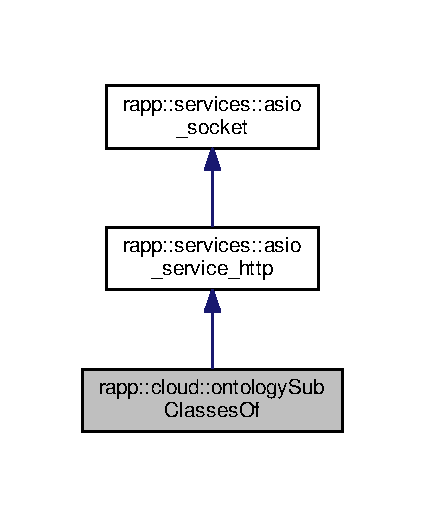
\includegraphics[width=204pt]{classrapp_1_1cloud_1_1ontologySubClassesOf__inherit__graph}
\end{center}
\end{figure}


Collaboration diagram for rapp\-:\-:cloud\-:\-:ontology\-Sub\-Classes\-Of\-:
\nopagebreak
\begin{figure}[H]
\begin{center}
\leavevmode
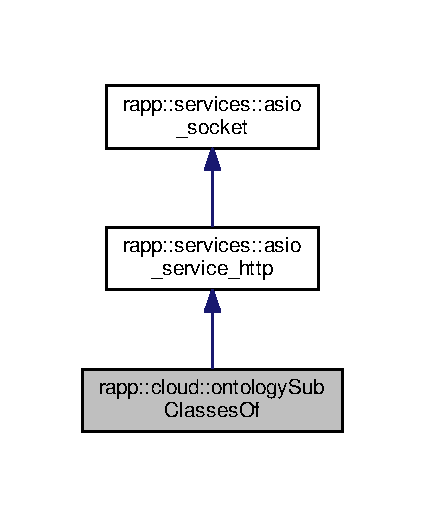
\includegraphics[width=204pt]{classrapp_1_1cloud_1_1ontologySubClassesOf__coll__graph}
\end{center}
\end{figure}
\subsection*{Public Member Functions}
\begin{DoxyCompactItemize}
\item 
\hyperlink{classrapp_1_1cloud_1_1ontologySubClassesOf_a2da927fee24f214627ab82532d772cd4}{ontology\-Sub\-Classes\-Of} (std\-::string query, std\-::function$<$ void(std\-::vector$<$ std\-::string $>$) $>$ callback)
\begin{DoxyCompactList}\small\item\em Constructor for this handler. \end{DoxyCompactList}\end{DoxyCompactItemize}
\subsection*{Private Member Functions}
\begin{DoxyCompactItemize}
\item 
void \hyperlink{classrapp_1_1cloud_1_1ontologySubClassesOf_addae350460d397612af1101f7b2baee9}{handle\-\_\-reply} (std\-::string json)
\end{DoxyCompactItemize}
\subsection*{Private Attributes}
\begin{DoxyCompactItemize}
\item 
std\-::function$<$ void(std\-::vector\\*
$<$ std\-::string $>$ classes) $>$ \hyperlink{classrapp_1_1cloud_1_1ontologySubClassesOf_a5f4e4ad83ac61ccd91871f1c3d4147b8}{delegate\-\_\-\-\_\-}
\begin{DoxyCompactList}\small\item\em The callback called upon completion of receiving the detected faces. \end{DoxyCompactList}\end{DoxyCompactItemize}
\subsection*{Additional Inherited Members}


\subsection{Detailed Description}


Definition at line 15 of file ontology\-Sub\-Classes\-Of.\-hpp.



\subsection{Constructor \& Destructor Documentation}
\hypertarget{classrapp_1_1cloud_1_1ontologySubClassesOf_a2da927fee24f214627ab82532d772cd4}{\index{rapp\-::cloud\-::ontology\-Sub\-Classes\-Of@{rapp\-::cloud\-::ontology\-Sub\-Classes\-Of}!ontology\-Sub\-Classes\-Of@{ontology\-Sub\-Classes\-Of}}
\index{ontology\-Sub\-Classes\-Of@{ontology\-Sub\-Classes\-Of}!rapp::cloud::ontologySubClassesOf@{rapp\-::cloud\-::ontology\-Sub\-Classes\-Of}}
\subsubsection[{ontology\-Sub\-Classes\-Of}]{\setlength{\rightskip}{0pt plus 5cm}rapp\-::cloud\-::ontology\-Sub\-Classes\-Of\-::ontology\-Sub\-Classes\-Of (
\begin{DoxyParamCaption}
\item[{std\-::string}]{query, }
\item[{std\-::function$<$ void(std\-::vector$<$ std\-::string $>$) $>$}]{callback}
\end{DoxyParamCaption}
)}}\label{classrapp_1_1cloud_1_1ontologySubClassesOf_a2da927fee24f214627ab82532d772cd4}


Constructor for this handler. 


\begin{DoxyParams}{Parameters}
{\em query} & is the entity for which we will try to acquire its Super-\/\-Ordinates \\
\hline
{\em callback} & is the functor that will receive the classes discovered \\
\hline
\end{DoxyParams}


Definition at line 25 of file ontology\-Sub\-Classes\-Of.\-hpp.



\subsection{Member Function Documentation}
\hypertarget{classrapp_1_1cloud_1_1ontologySubClassesOf_addae350460d397612af1101f7b2baee9}{\index{rapp\-::cloud\-::ontology\-Sub\-Classes\-Of@{rapp\-::cloud\-::ontology\-Sub\-Classes\-Of}!handle\-\_\-reply@{handle\-\_\-reply}}
\index{handle\-\_\-reply@{handle\-\_\-reply}!rapp::cloud::ontologySubClassesOf@{rapp\-::cloud\-::ontology\-Sub\-Classes\-Of}}
\subsubsection[{handle\-\_\-reply}]{\setlength{\rightskip}{0pt plus 5cm}void rapp\-::cloud\-::ontology\-Sub\-Classes\-Of\-::handle\-\_\-reply (
\begin{DoxyParamCaption}
\item[{std\-::string}]{json}
\end{DoxyParamCaption}
)\hspace{0.3cm}{\ttfamily [private]}}}\label{classrapp_1_1cloud_1_1ontologySubClassesOf_addae350460d397612af1101f7b2baee9}


Definition at line 44 of file ontology\-Sub\-Classes\-Of.\-hpp.



\subsection{Member Data Documentation}
\hypertarget{classrapp_1_1cloud_1_1ontologySubClassesOf_a5f4e4ad83ac61ccd91871f1c3d4147b8}{\index{rapp\-::cloud\-::ontology\-Sub\-Classes\-Of@{rapp\-::cloud\-::ontology\-Sub\-Classes\-Of}!delegate\-\_\-\-\_\-@{delegate\-\_\-\-\_\-}}
\index{delegate\-\_\-\-\_\-@{delegate\-\_\-\-\_\-}!rapp::cloud::ontologySubClassesOf@{rapp\-::cloud\-::ontology\-Sub\-Classes\-Of}}
\subsubsection[{delegate\-\_\-\-\_\-}]{\setlength{\rightskip}{0pt plus 5cm}std\-::function$<$ void( std\-::vector$<$std\-::string$>$ classes ) $>$ rapp\-::cloud\-::ontology\-Sub\-Classes\-Of\-::delegate\-\_\-\-\_\-\hspace{0.3cm}{\ttfamily [private]}}}\label{classrapp_1_1cloud_1_1ontologySubClassesOf_a5f4e4ad83ac61ccd91871f1c3d4147b8}


The callback called upon completion of receiving the detected faces. 



Definition at line 76 of file ontology\-Sub\-Classes\-Of.\-hpp.



The documentation for this class was generated from the following file\-:\begin{DoxyCompactItemize}
\item 
/home/travis/rapp\-\_\-temp/rapp-\/api/cpp/includes/cloud/ontology\-Sub\-Classes\-Of/\hyperlink{ontologySubClassesOf_8hpp}{ontology\-Sub\-Classes\-Of.\-hpp}\end{DoxyCompactItemize}

\hypertarget{classontologySubclassOf}{\section{ontology\-Subclass\-Of Class Reference}
\label{classontologySubclassOf}\index{ontology\-Subclass\-Of@{ontology\-Subclass\-Of}}
}


Asynchronous Service which will request the Ontology Subclass of/for an Input.  




{\ttfamily \#include $<$ontology\-Sub\-Classes\-Of.\-hpp$>$}



\subsection{Detailed Description}
Asynchronous Service which will request the Ontology Subclass of/for an Input. 

\begin{DoxyVersion}{Version}
3 
\end{DoxyVersion}
\begin{DoxyDate}{Date}
19-\/\-September-\/2015 
\end{DoxyDate}
\begin{DoxyAuthor}{Author}
Alex Gkiokas \href{mailto:a.gkiokas@ortelio.co.uk}{\tt a.\-gkiokas@ortelio.\-co.\-uk} H\-T\-T\-P P\-O\-S\-T R\-F\-C\-: \href{http://www.w3.org/Protocols/rfc2616/rfc2616-sec9.html}{\tt http\-://www.\-w3.\-org/\-Protocols/rfc2616/rfc2616-\/sec9.\-html} H\-T\-T\-P Transfer requirements\-: \href{http://www.w3.org/Protocols/rfc2616/rfc2616-sec8.html}{\tt http\-://www.\-w3.\-org/\-Protocols/rfc2616/rfc2616-\/sec8.\-html} 
\end{DoxyAuthor}


The documentation for this class was generated from the following file\-:\begin{DoxyCompactItemize}
\item 
/home/travis/rapp\-\_\-temp/rapp-\/api/cpp/includes/cloud/ontology\-Sub\-Classes\-Of/\hyperlink{ontologySubClassesOf_8hpp}{ontology\-Sub\-Classes\-Of.\-hpp}\end{DoxyCompactItemize}

\hypertarget{classontologySubSuperclassOf}{\section{ontology\-Sub\-Superclass\-Of Class Reference}
\label{classontologySubSuperclassOf}\index{ontology\-Sub\-Superclass\-Of@{ontology\-Sub\-Superclass\-Of}}
}


{\ttfamily \#include $<$ontology\-Is\-Sub\-Super\-Class\-Of.\-hpp$>$}



\subsection{Detailed Description}
\begin{DoxyVersion}{Version}

\end{DoxyVersion}
\begin{DoxyDate}{Date}

\end{DoxyDate}
\begin{DoxyAuthor}{Author}
Alex Gkiokas \href{mailto:a.gkiokas@ortelio.co.uk}{\tt a.\-gkiokas@ortelio.\-co.\-uk} 
\end{DoxyAuthor}


The documentation for this class was generated from the following file\-:\begin{DoxyCompactItemize}
\item 
/home/travis/rapp\-\_\-temp/rapp-\/api/cpp/includes/cloud/ontology\-Is\-Sub\-Super\-Class\-Of/\hyperlink{ontologyIsSubSuperClassOf_8hpp}{ontology\-Is\-Sub\-Super\-Class\-Of.\-hpp}\end{DoxyCompactItemize}

\hypertarget{classrapp_1_1cloud_1_1ontologySuperClassesOf}{\section{rapp\-:\-:cloud\-:\-:ontology\-Super\-Classes\-Of Class Reference}
\label{classrapp_1_1cloud_1_1ontologySuperClassesOf}\index{rapp\-::cloud\-::ontology\-Super\-Classes\-Of@{rapp\-::cloud\-::ontology\-Super\-Classes\-Of}}
}


{\ttfamily \#include $<$ontology\-Super\-Classes\-Of.\-hpp$>$}



Inheritance diagram for rapp\-:\-:cloud\-:\-:ontology\-Super\-Classes\-Of\-:
\nopagebreak
\begin{figure}[H]
\begin{center}
\leavevmode
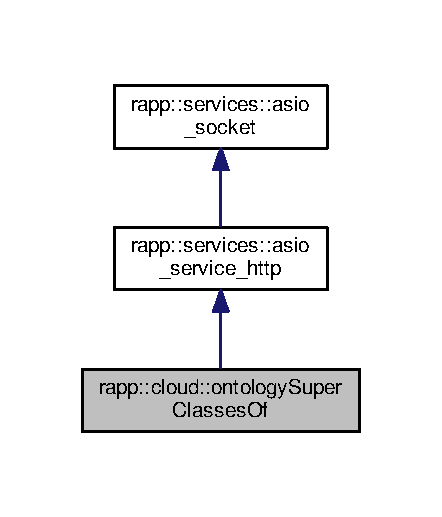
\includegraphics[width=212pt]{classrapp_1_1cloud_1_1ontologySuperClassesOf__inherit__graph}
\end{center}
\end{figure}


Collaboration diagram for rapp\-:\-:cloud\-:\-:ontology\-Super\-Classes\-Of\-:
\nopagebreak
\begin{figure}[H]
\begin{center}
\leavevmode
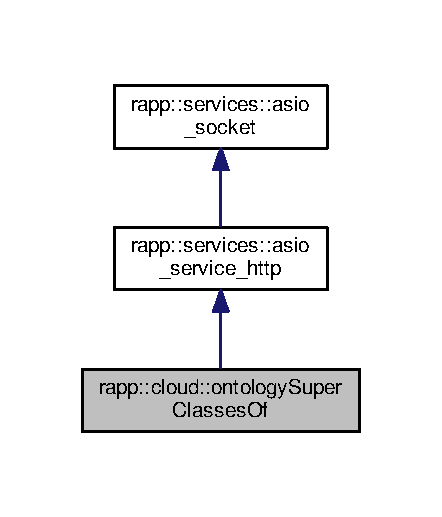
\includegraphics[width=212pt]{classrapp_1_1cloud_1_1ontologySuperClassesOf__coll__graph}
\end{center}
\end{figure}
\subsection*{Public Member Functions}
\begin{DoxyCompactItemize}
\item 
\hyperlink{classrapp_1_1cloud_1_1ontologySuperClassesOf_ad3deb8a1a1f303c6f721d92b9ee2553c}{ontology\-Super\-Classes\-Of} (const std\-::string query, std\-::function$<$ void(std\-::vector$<$ std\-::string $>$) $>$ callback)
\begin{DoxyCompactList}\small\item\em Constructor for this handler. \end{DoxyCompactList}\end{DoxyCompactItemize}
\subsection*{Private Member Functions}
\begin{DoxyCompactItemize}
\item 
void \hyperlink{classrapp_1_1cloud_1_1ontologySuperClassesOf_a4f4933a8220fde2be18e180be5ade709}{handle\-\_\-reply} (std\-::string json)
\end{DoxyCompactItemize}
\subsection*{Private Attributes}
\begin{DoxyCompactItemize}
\item 
std\-::function$<$ void(std\-::vector\\*
$<$ std\-::string $>$ classes) $>$ \hyperlink{classrapp_1_1cloud_1_1ontologySuperClassesOf_a44ae0e4c6d33f39b3161ee263b585604}{delegate\-\_\-\-\_\-}
\begin{DoxyCompactList}\small\item\em The callback called upon completion of receiving the detected faces. \end{DoxyCompactList}\end{DoxyCompactItemize}
\subsection*{Additional Inherited Members}


\subsection{Detailed Description}


Definition at line 13 of file ontology\-Super\-Classes\-Of.\-hpp.



\subsection{Constructor \& Destructor Documentation}
\hypertarget{classrapp_1_1cloud_1_1ontologySuperClassesOf_ad3deb8a1a1f303c6f721d92b9ee2553c}{\index{rapp\-::cloud\-::ontology\-Super\-Classes\-Of@{rapp\-::cloud\-::ontology\-Super\-Classes\-Of}!ontology\-Super\-Classes\-Of@{ontology\-Super\-Classes\-Of}}
\index{ontology\-Super\-Classes\-Of@{ontology\-Super\-Classes\-Of}!rapp::cloud::ontologySuperClassesOf@{rapp\-::cloud\-::ontology\-Super\-Classes\-Of}}
\subsubsection[{ontology\-Super\-Classes\-Of}]{\setlength{\rightskip}{0pt plus 5cm}rapp\-::cloud\-::ontology\-Super\-Classes\-Of\-::ontology\-Super\-Classes\-Of (
\begin{DoxyParamCaption}
\item[{const std\-::string}]{query, }
\item[{std\-::function$<$ void(std\-::vector$<$ std\-::string $>$) $>$}]{callback}
\end{DoxyParamCaption}
)}}\label{classrapp_1_1cloud_1_1ontologySuperClassesOf_ad3deb8a1a1f303c6f721d92b9ee2553c}


Constructor for this handler. 


\begin{DoxyParams}{Parameters}
{\em query} & is the entity for which we will try to acquire its Super-\/\-Ordinates \\
\hline
{\em callback} & is the functor that will receive the classes discovered \\
\hline
\end{DoxyParams}


Definition at line 22 of file ontology\-Super\-Classes\-Of.\-hpp.



\subsection{Member Function Documentation}
\hypertarget{classrapp_1_1cloud_1_1ontologySuperClassesOf_a4f4933a8220fde2be18e180be5ade709}{\index{rapp\-::cloud\-::ontology\-Super\-Classes\-Of@{rapp\-::cloud\-::ontology\-Super\-Classes\-Of}!handle\-\_\-reply@{handle\-\_\-reply}}
\index{handle\-\_\-reply@{handle\-\_\-reply}!rapp::cloud::ontologySuperClassesOf@{rapp\-::cloud\-::ontology\-Super\-Classes\-Of}}
\subsubsection[{handle\-\_\-reply}]{\setlength{\rightskip}{0pt plus 5cm}void rapp\-::cloud\-::ontology\-Super\-Classes\-Of\-::handle\-\_\-reply (
\begin{DoxyParamCaption}
\item[{std\-::string}]{json}
\end{DoxyParamCaption}
)\hspace{0.3cm}{\ttfamily [private]}}}\label{classrapp_1_1cloud_1_1ontologySuperClassesOf_a4f4933a8220fde2be18e180be5ade709}


Definition at line 40 of file ontology\-Super\-Classes\-Of.\-hpp.



\subsection{Member Data Documentation}
\hypertarget{classrapp_1_1cloud_1_1ontologySuperClassesOf_a44ae0e4c6d33f39b3161ee263b585604}{\index{rapp\-::cloud\-::ontology\-Super\-Classes\-Of@{rapp\-::cloud\-::ontology\-Super\-Classes\-Of}!delegate\-\_\-\-\_\-@{delegate\-\_\-\-\_\-}}
\index{delegate\-\_\-\-\_\-@{delegate\-\_\-\-\_\-}!rapp::cloud::ontologySuperClassesOf@{rapp\-::cloud\-::ontology\-Super\-Classes\-Of}}
\subsubsection[{delegate\-\_\-\-\_\-}]{\setlength{\rightskip}{0pt plus 5cm}std\-::function$<$ void( std\-::vector$<$std\-::string$>$ classes ) $>$ rapp\-::cloud\-::ontology\-Super\-Classes\-Of\-::delegate\-\_\-\-\_\-\hspace{0.3cm}{\ttfamily [private]}}}\label{classrapp_1_1cloud_1_1ontologySuperClassesOf_a44ae0e4c6d33f39b3161ee263b585604}


The callback called upon completion of receiving the detected faces. 



Definition at line 73 of file ontology\-Super\-Classes\-Of.\-hpp.



The documentation for this class was generated from the following file\-:\begin{DoxyCompactItemize}
\item 
/home/travis/rapp\-\_\-temp/rapp-\/api/cpp/includes/cloud/ontology\-Super\-Classes\-Of/\hyperlink{ontologySuperClassesOf_8hpp}{ontology\-Super\-Classes\-Of.\-hpp}\end{DoxyCompactItemize}

\hypertarget{classontologySuperclassesOf}{\section{ontology\-Superclasses\-Of Class Reference}
\label{classontologySuperclassesOf}\index{ontology\-Superclasses\-Of@{ontology\-Superclasses\-Of}}
}


{\ttfamily \#include $<$ontology\-Super\-Classes\-Of.\-hpp$>$}



\subsection{Detailed Description}
\begin{DoxyVersion}{Version}

\end{DoxyVersion}
\begin{DoxyDate}{Date}

\end{DoxyDate}
\begin{DoxyAuthor}{Author}
Alex Gkiokas \href{mailto:a.gkiokas@ortelio.co.uk}{\tt a.\-gkiokas@ortelio.\-co.\-uk} 
\end{DoxyAuthor}


The documentation for this class was generated from the following file\-:\begin{DoxyCompactItemize}
\item 
/home/travis/rapp\-\_\-temp/rapp-\/api/cpp/includes/cloud/ontology\-Super\-Classes\-Of/\hyperlink{ontologySuperClassesOf_8hpp}{ontology\-Super\-Classes\-Of.\-hpp}\end{DoxyCompactItemize}

\hypertarget{classrapp_1_1object_1_1picture}{\section{rapp\-:\-:object\-:\-:picture Class Reference}
\label{classrapp_1_1object_1_1picture}\index{rapp\-::object\-::picture@{rapp\-::object\-::picture}}
}


class which wraps around raw bytes of a picture  




{\ttfamily \#include $<$picture.\-hpp$>$}

\subsection*{Public Member Functions}
\begin{DoxyCompactItemize}
\item 
\hyperlink{classrapp_1_1object_1_1picture_a037d64b0a69603a9ad624760cf2b1072}{picture} (const std\-::string filepath)
\begin{DoxyCompactList}\small\item\em Construct from a file-\/path. \end{DoxyCompactList}\item 
\hyperlink{classrapp_1_1object_1_1picture_a20da2075d7f03172258584b2ad8f2fb3}{picture} (std\-::ifstream \&bytestream)
\begin{DoxyCompactList}\small\item\em Construct using an open file stream. \end{DoxyCompactList}\item 
\hyperlink{classrapp_1_1object_1_1picture_a9e0aa9a62b6455d542eb14705d2be6fe}{picture} (const \hyperlink{classrapp_1_1object_1_1picture}{picture} \&)=default
\begin{DoxyCompactList}\small\item\em Copy constructor. \end{DoxyCompactList}\item 
std\-::vector$<$ \hyperlink{namespacerapp_1_1types_a1dbc9dc2ab4507d8fb58ac3a204d307b}{rapp\-::types\-::byte} $>$ \hyperlink{classrapp_1_1object_1_1picture_a27bd4bd6bb318e2a1866c3aa7c4d66a5}{bytearray} () const 
\begin{DoxyCompactList}\small\item\em Get picture as array of bytes. \end{DoxyCompactList}\item 
\hyperlink{classrapp_1_1object_1_1picture}{picture} \& \hyperlink{classrapp_1_1object_1_1picture_a312b1e70d3e4af4f4a8ce8fc98b19afa}{operator=} (const \hyperlink{classrapp_1_1object_1_1picture}{picture} \&)=default
\begin{DoxyCompactList}\small\item\em Assignment operator. \end{DoxyCompactList}\item 
bool \hyperlink{classrapp_1_1object_1_1picture_aad6e18da0e6be9ad7d195ee34b79bf2c}{operator==} (const \hyperlink{classrapp_1_1object_1_1picture}{picture} \&rhs) const 
\begin{DoxyCompactList}\small\item\em Are pictures same ? \end{DoxyCompactList}\item 
bool \hyperlink{classrapp_1_1object_1_1picture_afc2c1e50bd6192da8ee1588e3969a669}{save} (const std\-::string filepath)
\begin{DoxyCompactList}\small\item\em Save picture to filepath. \end{DoxyCompactList}\end{DoxyCompactItemize}
\subsection*{Private Member Functions}
\begin{DoxyCompactItemize}
\item 
\hyperlink{classrapp_1_1object_1_1picture_a4edfc5d343a51a181c743d76d18c10f9}{picture} ()=delete
\item 
void \hyperlink{classrapp_1_1object_1_1picture_aefe39dd6c7f1ef438e8232881c6450e1}{open\-Copy\-\_\-} (std\-::ifstream \&bytestream)
\end{DoxyCompactItemize}
\subsection*{Private Attributes}
\begin{DoxyCompactItemize}
\item 
std\-::vector$<$ \hyperlink{namespacerapp_1_1types_a1dbc9dc2ab4507d8fb58ac3a204d307b}{rapp\-::types\-::byte} $>$ \hyperlink{classrapp_1_1object_1_1picture_a4c6377918f2286dbbe320cd9a1d8767c}{bytearray\-\_\-}
\end{DoxyCompactItemize}


\subsection{Detailed Description}
class which wraps around raw bytes of a picture 

\begin{DoxyVersion}{Version}
2 
\end{DoxyVersion}
\begin{DoxyDate}{Date}
6-\/\-February-\/2015 
\end{DoxyDate}
\begin{DoxyAuthor}{Author}
Alex Gkiokas \href{mailto:a.gkiokas@ortelio.co.uk}{\tt a.\-gkiokas@ortelio.\-co.\-uk} 
\end{DoxyAuthor}


Definition at line 13 of file picture.\-hpp.



\subsection{Constructor \& Destructor Documentation}
\hypertarget{classrapp_1_1object_1_1picture_a037d64b0a69603a9ad624760cf2b1072}{\index{rapp\-::object\-::picture@{rapp\-::object\-::picture}!picture@{picture}}
\index{picture@{picture}!rapp::object::picture@{rapp\-::object\-::picture}}
\subsubsection[{picture}]{\setlength{\rightskip}{0pt plus 5cm}rapp\-::object\-::picture\-::picture (
\begin{DoxyParamCaption}
\item[{const std\-::string}]{filepath}
\end{DoxyParamCaption}
)}}\label{classrapp_1_1object_1_1picture_a037d64b0a69603a9ad624760cf2b1072}


Construct from a file-\/path. 



Definition at line 18 of file picture.\-hpp.

\hypertarget{classrapp_1_1object_1_1picture_a20da2075d7f03172258584b2ad8f2fb3}{\index{rapp\-::object\-::picture@{rapp\-::object\-::picture}!picture@{picture}}
\index{picture@{picture}!rapp::object::picture@{rapp\-::object\-::picture}}
\subsubsection[{picture}]{\setlength{\rightskip}{0pt plus 5cm}rapp\-::object\-::picture\-::picture (
\begin{DoxyParamCaption}
\item[{std\-::ifstream \&}]{bytestream}
\end{DoxyParamCaption}
)}}\label{classrapp_1_1object_1_1picture_a20da2075d7f03172258584b2ad8f2fb3}


Construct using an open file stream. 



Definition at line 29 of file picture.\-hpp.

\hypertarget{classrapp_1_1object_1_1picture_a9e0aa9a62b6455d542eb14705d2be6fe}{\index{rapp\-::object\-::picture@{rapp\-::object\-::picture}!picture@{picture}}
\index{picture@{picture}!rapp::object::picture@{rapp\-::object\-::picture}}
\subsubsection[{picture}]{\setlength{\rightskip}{0pt plus 5cm}rapp\-::object\-::picture\-::picture (
\begin{DoxyParamCaption}
\item[{const {\bf picture} \&}]{}
\end{DoxyParamCaption}
)\hspace{0.3cm}{\ttfamily [default]}}}\label{classrapp_1_1object_1_1picture_a9e0aa9a62b6455d542eb14705d2be6fe}


Copy constructor. 

\hypertarget{classrapp_1_1object_1_1picture_a4edfc5d343a51a181c743d76d18c10f9}{\index{rapp\-::object\-::picture@{rapp\-::object\-::picture}!picture@{picture}}
\index{picture@{picture}!rapp::object::picture@{rapp\-::object\-::picture}}
\subsubsection[{picture}]{\setlength{\rightskip}{0pt plus 5cm}rapp\-::object\-::picture\-::picture (
\begin{DoxyParamCaption}
{}
\end{DoxyParamCaption}
)\hspace{0.3cm}{\ttfamily [private]}, {\ttfamily [delete]}}}\label{classrapp_1_1object_1_1picture_a4edfc5d343a51a181c743d76d18c10f9}


\subsection{Member Function Documentation}
\hypertarget{classrapp_1_1object_1_1picture_a27bd4bd6bb318e2a1866c3aa7c4d66a5}{\index{rapp\-::object\-::picture@{rapp\-::object\-::picture}!bytearray@{bytearray}}
\index{bytearray@{bytearray}!rapp::object::picture@{rapp\-::object\-::picture}}
\subsubsection[{bytearray}]{\setlength{\rightskip}{0pt plus 5cm}std\-::vector$<${\bf rapp\-::types\-::byte}$>$ rapp\-::object\-::picture\-::bytearray (
\begin{DoxyParamCaption}
{}
\end{DoxyParamCaption}
) const}}\label{classrapp_1_1object_1_1picture_a27bd4bd6bb318e2a1866c3aa7c4d66a5}


Get picture as array of bytes. 



Definition at line 38 of file picture.\-hpp.

\hypertarget{classrapp_1_1object_1_1picture_aefe39dd6c7f1ef438e8232881c6450e1}{\index{rapp\-::object\-::picture@{rapp\-::object\-::picture}!open\-Copy\-\_\-@{open\-Copy\-\_\-}}
\index{open\-Copy\-\_\-@{open\-Copy\-\_\-}!rapp::object::picture@{rapp\-::object\-::picture}}
\subsubsection[{open\-Copy\-\_\-}]{\setlength{\rightskip}{0pt plus 5cm}void rapp\-::object\-::picture\-::open\-Copy\-\_\- (
\begin{DoxyParamCaption}
\item[{std\-::ifstream \&}]{bytestream}
\end{DoxyParamCaption}
)\hspace{0.3cm}{\ttfamily [private]}}}\label{classrapp_1_1object_1_1picture_aefe39dd6c7f1ef438e8232881c6450e1}


Definition at line 73 of file picture.\-hpp.

\hypertarget{classrapp_1_1object_1_1picture_a312b1e70d3e4af4f4a8ce8fc98b19afa}{\index{rapp\-::object\-::picture@{rapp\-::object\-::picture}!operator=@{operator=}}
\index{operator=@{operator=}!rapp::object::picture@{rapp\-::object\-::picture}}
\subsubsection[{operator=}]{\setlength{\rightskip}{0pt plus 5cm}{\bf picture}\& rapp\-::object\-::picture\-::operator= (
\begin{DoxyParamCaption}
\item[{const {\bf picture} \&}]{}
\end{DoxyParamCaption}
)\hspace{0.3cm}{\ttfamily [default]}}}\label{classrapp_1_1object_1_1picture_a312b1e70d3e4af4f4a8ce8fc98b19afa}


Assignment operator. 

\hypertarget{classrapp_1_1object_1_1picture_aad6e18da0e6be9ad7d195ee34b79bf2c}{\index{rapp\-::object\-::picture@{rapp\-::object\-::picture}!operator==@{operator==}}
\index{operator==@{operator==}!rapp::object::picture@{rapp\-::object\-::picture}}
\subsubsection[{operator==}]{\setlength{\rightskip}{0pt plus 5cm}bool rapp\-::object\-::picture\-::operator== (
\begin{DoxyParamCaption}
\item[{const {\bf picture} \&}]{rhs}
\end{DoxyParamCaption}
) const}}\label{classrapp_1_1object_1_1picture_aad6e18da0e6be9ad7d195ee34b79bf2c}


Are pictures same ? 



Definition at line 44 of file picture.\-hpp.

\hypertarget{classrapp_1_1object_1_1picture_afc2c1e50bd6192da8ee1588e3969a669}{\index{rapp\-::object\-::picture@{rapp\-::object\-::picture}!save@{save}}
\index{save@{save}!rapp::object::picture@{rapp\-::object\-::picture}}
\subsubsection[{save}]{\setlength{\rightskip}{0pt plus 5cm}bool rapp\-::object\-::picture\-::save (
\begin{DoxyParamCaption}
\item[{const std\-::string}]{filepath}
\end{DoxyParamCaption}
)}}\label{classrapp_1_1object_1_1picture_afc2c1e50bd6192da8ee1588e3969a669}


Save picture to filepath. 



Definition at line 53 of file picture.\-hpp.



\subsection{Member Data Documentation}
\hypertarget{classrapp_1_1object_1_1picture_a4c6377918f2286dbbe320cd9a1d8767c}{\index{rapp\-::object\-::picture@{rapp\-::object\-::picture}!bytearray\-\_\-@{bytearray\-\_\-}}
\index{bytearray\-\_\-@{bytearray\-\_\-}!rapp::object::picture@{rapp\-::object\-::picture}}
\subsubsection[{bytearray\-\_\-}]{\setlength{\rightskip}{0pt plus 5cm}std\-::vector$<${\bf rapp\-::types\-::byte}$>$ rapp\-::object\-::picture\-::bytearray\-\_\-\hspace{0.3cm}{\ttfamily [private]}}}\label{classrapp_1_1object_1_1picture_a4c6377918f2286dbbe320cd9a1d8767c}


Definition at line 83 of file picture.\-hpp.



The documentation for this class was generated from the following file\-:\begin{DoxyCompactItemize}
\item 
/home/travis/rapp\-\_\-temp/rapp-\/api/cpp/includes/objects/picture/\hyperlink{picture_8hpp}{picture.\-hpp}\end{DoxyCompactItemize}

\hypertarget{classrapp_1_1robot_1_1proto}{\section{rapp\-:\-:robot\-:\-:proto Class Reference}
\label{classrapp_1_1robot_1_1proto}\index{rapp\-::robot\-::proto@{rapp\-::robot\-::proto}}
}


Abstract Base Class (A\-B\-C) Interface Prototype for all Robots.  




{\ttfamily \#include $<$proto.\-hpp$>$}



Inheritance diagram for rapp\-:\-:robot\-:\-:proto\-:
\nopagebreak
\begin{figure}[H]
\begin{center}
\leavevmode
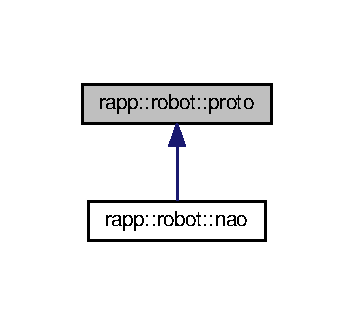
\includegraphics[width=170pt]{classrapp_1_1robot_1_1proto__inherit__graph}
\end{center}
\end{figure}
\subsection*{Public Member Functions}
\begin{DoxyCompactItemize}
\item 
virtual std\-::string \hyperlink{classrapp_1_1robot_1_1proto_ace501b12c79698041f37a90306163aa9}{model} () const =0
\begin{DoxyCompactList}\small\item\em Get Robot's Model. \end{DoxyCompactList}\item 
virtual std\-::string \hyperlink{classrapp_1_1robot_1_1proto_a2d0dd7d28350e8a7c6ffb7616c0a6f5f}{ruid} () const =0
\begin{DoxyCompactList}\small\item\em Get Robot's Unique I\-D. \end{DoxyCompactList}\end{DoxyCompactItemize}


\subsection{Detailed Description}
Abstract Base Class (A\-B\-C) Interface Prototype for all Robots. 

\begin{DoxyVersion}{Version}
1 
\end{DoxyVersion}
\begin{DoxyDate}{Date}
20-\/\-September-\/2015 
\end{DoxyDate}
\begin{DoxyAuthor}{Author}
Alex Gkiokas \href{mailto:a.gkiokas@ortelio.co.uk}{\tt a.\-gkiokas@ortelio.\-co.\-uk} 
\end{DoxyAuthor}


Definition at line 13 of file proto.\-hpp.



\subsection{Member Function Documentation}
\hypertarget{classrapp_1_1robot_1_1proto_ace501b12c79698041f37a90306163aa9}{\index{rapp\-::robot\-::proto@{rapp\-::robot\-::proto}!model@{model}}
\index{model@{model}!rapp::robot::proto@{rapp\-::robot\-::proto}}
\subsubsection[{model}]{\setlength{\rightskip}{0pt plus 5cm}virtual std\-::string rapp\-::robot\-::proto\-::model (
\begin{DoxyParamCaption}
{}
\end{DoxyParamCaption}
) const\hspace{0.3cm}{\ttfamily [pure virtual]}}}\label{classrapp_1_1robot_1_1proto_ace501b12c79698041f37a90306163aa9}


Get Robot's Model. 



Implemented in \hyperlink{classrapp_1_1robot_1_1nao_aed3ffea92e69e9e0fba684c42f5f7cfd}{rapp\-::robot\-::nao}.

\hypertarget{classrapp_1_1robot_1_1proto_a2d0dd7d28350e8a7c6ffb7616c0a6f5f}{\index{rapp\-::robot\-::proto@{rapp\-::robot\-::proto}!ruid@{ruid}}
\index{ruid@{ruid}!rapp::robot::proto@{rapp\-::robot\-::proto}}
\subsubsection[{ruid}]{\setlength{\rightskip}{0pt plus 5cm}virtual std\-::string rapp\-::robot\-::proto\-::ruid (
\begin{DoxyParamCaption}
{}
\end{DoxyParamCaption}
) const\hspace{0.3cm}{\ttfamily [pure virtual]}}}\label{classrapp_1_1robot_1_1proto_a2d0dd7d28350e8a7c6ffb7616c0a6f5f}


Get Robot's Unique I\-D. 



Implemented in \hyperlink{classrapp_1_1robot_1_1nao_a0eb438d37b7958554ba43b7b3cddf131}{rapp\-::robot\-::nao}.



The documentation for this class was generated from the following file\-:\begin{DoxyCompactItemize}
\item 
/home/travis/rapp\-\_\-temp/rapp-\/api/cpp/includes/robot/proto/\hyperlink{proto_8hpp}{proto.\-hpp}\end{DoxyCompactItemize}

\hypertarget{classrapp_1_1object_1_1qrCode}{\section{rapp\-:\-:object\-:\-:qr\-Code Class Reference}
\label{classrapp_1_1object_1_1qrCode}\index{rapp\-::object\-::qr\-Code@{rapp\-::object\-::qr\-Code}}
}


class which should encapsulate a Q\-R code  




{\ttfamily \#include $<$qr\-Code.\-hpp$>$}

\subsection*{Public Member Functions}
\begin{DoxyCompactItemize}
\item 
\hyperlink{classrapp_1_1object_1_1qrCode_a554b8eae4e757f48bc4b8448e81e59a1}{qr\-Code} (float centre\-\_\-x, float centre\-\_\-y, std\-::string \hyperlink{classrapp_1_1object_1_1qrCode_aa794b7ec326c02e576d18f4eefb1728b}{label})
\begin{DoxyCompactList}\small\item\em Consruct using code coordinates (a rectangle) and a label (U\-R\-L, email, string, etc) \end{DoxyCompactList}\item 
\hyperlink{classrapp_1_1object_1_1qrCode_ae1be3ca19c3264e6963ec8ccfdfb5c76}{qr\-Code} ()=default
\begin{DoxyCompactList}\small\item\em Allow Empty Consructor. \end{DoxyCompactList}\item 
\hyperlink{classrapp_1_1object_1_1qrCode_a3b640b791a571346951967a8971f8a65}{qr\-Code} (const \hyperlink{classrapp_1_1object_1_1qrCode}{qr\-Code} \&)=default
\begin{DoxyCompactList}\small\item\em Copy Conatructor. \end{DoxyCompactList}\item 
std\-::string \hyperlink{classrapp_1_1object_1_1qrCode_aa794b7ec326c02e576d18f4eefb1728b}{label} () const 
\begin{DoxyCompactList}\small\item\em Get the qr Label. \end{DoxyCompactList}\item 
bool \hyperlink{classrapp_1_1object_1_1qrCode_a5bee3345d72a2c9f72c1bc6f681264fb}{operator==} (const \hyperlink{classrapp_1_1object_1_1qrCode}{qr\-Code} \&rhs) const 
\begin{DoxyCompactList}\small\item\em Assignment Constructor. \end{DoxyCompactList}\end{DoxyCompactItemize}
\subsection*{Private Attributes}
\begin{DoxyCompactItemize}
\item 
float \hyperlink{classrapp_1_1object_1_1qrCode_a731e64161861c6dbcd83729564bf04c7}{centre\-\_\-x\-\_\-\-\_\-} = -\/1
\item 
float \hyperlink{classrapp_1_1object_1_1qrCode_ae6d1a8dcfd971d39405f11566613f4ec}{centre\-\_\-y\-\_\-\-\_\-} = -\/1
\item 
std\-::string \hyperlink{classrapp_1_1object_1_1qrCode_a890dfabeb0190571784cea1df0ca36b7}{message\-\_\-\-\_\-}
\end{DoxyCompactItemize}


\subsection{Detailed Description}
class which should encapsulate a Q\-R code 

\begin{DoxyVersion}{Version}
1 
\end{DoxyVersion}
\begin{DoxyDate}{Date}
13-\/\-February-\/2015 
\end{DoxyDate}
\begin{DoxyAuthor}{Author}
Alex Gkiokas \href{mailto:a.gkiokas@ortelio.co.uk}{\tt a.\-gkiokas@ortelio.\-co.\-uk} 
\end{DoxyAuthor}


Definition at line 16 of file qr\-Code.\-hpp.



\subsection{Constructor \& Destructor Documentation}
\hypertarget{classrapp_1_1object_1_1qrCode_a554b8eae4e757f48bc4b8448e81e59a1}{\index{rapp\-::object\-::qr\-Code@{rapp\-::object\-::qr\-Code}!qr\-Code@{qr\-Code}}
\index{qr\-Code@{qr\-Code}!rapp::object::qrCode@{rapp\-::object\-::qr\-Code}}
\subsubsection[{qr\-Code}]{\setlength{\rightskip}{0pt plus 5cm}rapp\-::object\-::qr\-Code\-::qr\-Code (
\begin{DoxyParamCaption}
\item[{float}]{centre\-\_\-x, }
\item[{float}]{centre\-\_\-y, }
\item[{std\-::string}]{label}
\end{DoxyParamCaption}
)}}\label{classrapp_1_1object_1_1qrCode_a554b8eae4e757f48bc4b8448e81e59a1}


Consruct using code coordinates (a rectangle) and a label (U\-R\-L, email, string, etc) 


\begin{DoxyParams}{Parameters}
{\em centre\-\_\-x} & is coordinate \\
\hline
{\em centre\-\_\-y} & is coordinate \\
\hline
{\em label} & is message embedded in Q\-R \\
\hline
\end{DoxyParams}


Definition at line 26 of file qr\-Code.\-hpp.

\hypertarget{classrapp_1_1object_1_1qrCode_ae1be3ca19c3264e6963ec8ccfdfb5c76}{\index{rapp\-::object\-::qr\-Code@{rapp\-::object\-::qr\-Code}!qr\-Code@{qr\-Code}}
\index{qr\-Code@{qr\-Code}!rapp::object::qrCode@{rapp\-::object\-::qr\-Code}}
\subsubsection[{qr\-Code}]{\setlength{\rightskip}{0pt plus 5cm}rapp\-::object\-::qr\-Code\-::qr\-Code (
\begin{DoxyParamCaption}
{}
\end{DoxyParamCaption}
)\hspace{0.3cm}{\ttfamily [default]}}}\label{classrapp_1_1object_1_1qrCode_ae1be3ca19c3264e6963ec8ccfdfb5c76}


Allow Empty Consructor. 

\hypertarget{classrapp_1_1object_1_1qrCode_a3b640b791a571346951967a8971f8a65}{\index{rapp\-::object\-::qr\-Code@{rapp\-::object\-::qr\-Code}!qr\-Code@{qr\-Code}}
\index{qr\-Code@{qr\-Code}!rapp::object::qrCode@{rapp\-::object\-::qr\-Code}}
\subsubsection[{qr\-Code}]{\setlength{\rightskip}{0pt plus 5cm}rapp\-::object\-::qr\-Code\-::qr\-Code (
\begin{DoxyParamCaption}
\item[{const {\bf qr\-Code} \&}]{}
\end{DoxyParamCaption}
)\hspace{0.3cm}{\ttfamily [default]}}}\label{classrapp_1_1object_1_1qrCode_a3b640b791a571346951967a8971f8a65}


Copy Conatructor. 



\subsection{Member Function Documentation}
\hypertarget{classrapp_1_1object_1_1qrCode_aa794b7ec326c02e576d18f4eefb1728b}{\index{rapp\-::object\-::qr\-Code@{rapp\-::object\-::qr\-Code}!label@{label}}
\index{label@{label}!rapp::object::qrCode@{rapp\-::object\-::qr\-Code}}
\subsubsection[{label}]{\setlength{\rightskip}{0pt plus 5cm}std\-::string rapp\-::object\-::qr\-Code\-::label (
\begin{DoxyParamCaption}
{}
\end{DoxyParamCaption}
) const}}\label{classrapp_1_1object_1_1qrCode_aa794b7ec326c02e576d18f4eefb1728b}


Get the qr Label. 



Definition at line 57 of file qr\-Code.\-hpp.

\hypertarget{classrapp_1_1object_1_1qrCode_a5bee3345d72a2c9f72c1bc6f681264fb}{\index{rapp\-::object\-::qr\-Code@{rapp\-::object\-::qr\-Code}!operator==@{operator==}}
\index{operator==@{operator==}!rapp::object::qrCode@{rapp\-::object\-::qr\-Code}}
\subsubsection[{operator==}]{\setlength{\rightskip}{0pt plus 5cm}bool rapp\-::object\-::qr\-Code\-::operator== (
\begin{DoxyParamCaption}
\item[{const {\bf qr\-Code} \&}]{rhs}
\end{DoxyParamCaption}
) const}}\label{classrapp_1_1object_1_1qrCode_a5bee3345d72a2c9f72c1bc6f681264fb}


Assignment Constructor. 

Equality operator \begin{DoxyNote}{Note}
only the message is compared (insensitive case), not the coordinates! 
\end{DoxyNote}


Definition at line 49 of file qr\-Code.\-hpp.



\subsection{Member Data Documentation}
\hypertarget{classrapp_1_1object_1_1qrCode_a731e64161861c6dbcd83729564bf04c7}{\index{rapp\-::object\-::qr\-Code@{rapp\-::object\-::qr\-Code}!centre\-\_\-x\-\_\-\-\_\-@{centre\-\_\-x\-\_\-\-\_\-}}
\index{centre\-\_\-x\-\_\-\-\_\-@{centre\-\_\-x\-\_\-\-\_\-}!rapp::object::qrCode@{rapp\-::object\-::qr\-Code}}
\subsubsection[{centre\-\_\-x\-\_\-\-\_\-}]{\setlength{\rightskip}{0pt plus 5cm}float rapp\-::object\-::qr\-Code\-::centre\-\_\-x\-\_\-\-\_\- = -\/1\hspace{0.3cm}{\ttfamily [private]}}}\label{classrapp_1_1object_1_1qrCode_a731e64161861c6dbcd83729564bf04c7}


Definition at line 64 of file qr\-Code.\-hpp.

\hypertarget{classrapp_1_1object_1_1qrCode_ae6d1a8dcfd971d39405f11566613f4ec}{\index{rapp\-::object\-::qr\-Code@{rapp\-::object\-::qr\-Code}!centre\-\_\-y\-\_\-\-\_\-@{centre\-\_\-y\-\_\-\-\_\-}}
\index{centre\-\_\-y\-\_\-\-\_\-@{centre\-\_\-y\-\_\-\-\_\-}!rapp::object::qrCode@{rapp\-::object\-::qr\-Code}}
\subsubsection[{centre\-\_\-y\-\_\-\-\_\-}]{\setlength{\rightskip}{0pt plus 5cm}float rapp\-::object\-::qr\-Code\-::centre\-\_\-y\-\_\-\-\_\- = -\/1\hspace{0.3cm}{\ttfamily [private]}}}\label{classrapp_1_1object_1_1qrCode_ae6d1a8dcfd971d39405f11566613f4ec}


Definition at line 66 of file qr\-Code.\-hpp.

\hypertarget{classrapp_1_1object_1_1qrCode_a890dfabeb0190571784cea1df0ca36b7}{\index{rapp\-::object\-::qr\-Code@{rapp\-::object\-::qr\-Code}!message\-\_\-\-\_\-@{message\-\_\-\-\_\-}}
\index{message\-\_\-\-\_\-@{message\-\_\-\-\_\-}!rapp::object::qrCode@{rapp\-::object\-::qr\-Code}}
\subsubsection[{message\-\_\-\-\_\-}]{\setlength{\rightskip}{0pt plus 5cm}std\-::string rapp\-::object\-::qr\-Code\-::message\-\_\-\-\_\-\hspace{0.3cm}{\ttfamily [private]}}}\label{classrapp_1_1object_1_1qrCode_a890dfabeb0190571784cea1df0ca36b7}


Definition at line 68 of file qr\-Code.\-hpp.



The documentation for this class was generated from the following file\-:\begin{DoxyCompactItemize}
\item 
/home/travis/rapp\-\_\-temp/rapp-\/api/cpp/includes/objects/qr\-Code/\hyperlink{qrCode_8hpp}{qr\-Code.\-hpp}\end{DoxyCompactItemize}

\hypertarget{classrapp_1_1cloud_1_1qrDetector}{\section{rapp\-:\-:cloud\-:\-:qr\-Detector Class Reference}
\label{classrapp_1_1cloud_1_1qrDetector}\index{rapp\-::cloud\-::qr\-Detector@{rapp\-::cloud\-::qr\-Detector}}
}


Asynchronous Service which will request the cloud to detect Q\-R codes.  




{\ttfamily \#include $<$qr\-Detector.\-hpp$>$}



Inheritance diagram for rapp\-:\-:cloud\-:\-:qr\-Detector\-:
\nopagebreak
\begin{figure}[H]
\begin{center}
\leavevmode
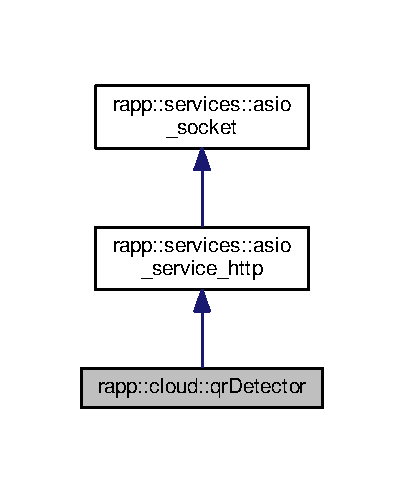
\includegraphics[width=194pt]{classrapp_1_1cloud_1_1qrDetector__inherit__graph}
\end{center}
\end{figure}


Collaboration diagram for rapp\-:\-:cloud\-:\-:qr\-Detector\-:
\nopagebreak
\begin{figure}[H]
\begin{center}
\leavevmode
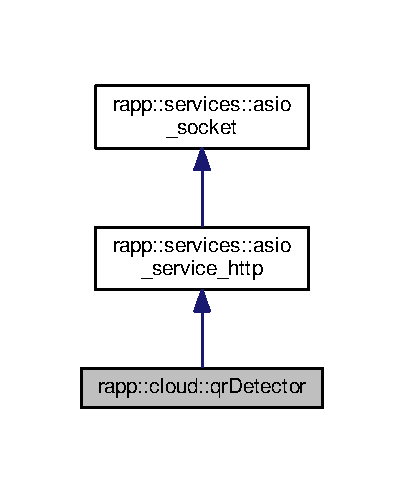
\includegraphics[width=194pt]{classrapp_1_1cloud_1_1qrDetector__coll__graph}
\end{center}
\end{figure}
\subsection*{Public Member Functions}
\begin{DoxyCompactItemize}
\item 
\hyperlink{classrapp_1_1cloud_1_1qrDetector_aec014d825c4cc07867efbc9ed68570eb}{qr\-Detector} (const std\-::shared\-\_\-ptr$<$ \hyperlink{classrapp_1_1object_1_1picture}{rapp\-::object\-::picture} $>$ image, const std\-::string image\-\_\-format, std\-::function$<$ void(std\-::vector$<$ \hyperlink{classrapp_1_1object_1_1qrCode}{rapp\-::object\-::qr\-Code} $>$) $>$ callback)
\begin{DoxyCompactList}\small\item\em Constructor. \end{DoxyCompactList}\end{DoxyCompactItemize}
\subsection*{Private Member Functions}
\begin{DoxyCompactItemize}
\item 
void \hyperlink{classrapp_1_1cloud_1_1qrDetector_ae604fb59970ea287bff8be0fc8c5eb4c}{handle\-\_\-reply} (std\-::string json)
\end{DoxyCompactItemize}
\subsection*{Private Attributes}
\begin{DoxyCompactItemize}
\item 
std\-::function$<$ void(std\-::vector\\*
$<$ \hyperlink{classrapp_1_1object_1_1qrCode}{rapp\-::object\-::qr\-Code} $>$) $>$ \hyperlink{classrapp_1_1cloud_1_1qrDetector_a5a835964ee4db7bac1fe7412d242c445}{delegate\-\_\-\-\_\-}
\begin{DoxyCompactList}\small\item\em The callback called upon completion of receiving the detected faces. \end{DoxyCompactList}\end{DoxyCompactItemize}
\subsection*{Additional Inherited Members}


\subsection{Detailed Description}
Asynchronous Service which will request the cloud to detect Q\-R codes. 

\begin{DoxyVersion}{Version}
2 
\end{DoxyVersion}
\begin{DoxyDate}{Date}
26-\/\-April-\/2015 
\end{DoxyDate}
\begin{DoxyAuthor}{Author}
Alex Gkiokas \href{mailto:a.gkiokas@ortelio.co.uk}{\tt a.\-gkiokas@ortelio.\-co.\-uk} 
\end{DoxyAuthor}


Definition at line 13 of file qr\-Detector.\-hpp.



\subsection{Constructor \& Destructor Documentation}
\hypertarget{classrapp_1_1cloud_1_1qrDetector_aec014d825c4cc07867efbc9ed68570eb}{\index{rapp\-::cloud\-::qr\-Detector@{rapp\-::cloud\-::qr\-Detector}!qr\-Detector@{qr\-Detector}}
\index{qr\-Detector@{qr\-Detector}!rapp::cloud::qrDetector@{rapp\-::cloud\-::qr\-Detector}}
\subsubsection[{qr\-Detector}]{\setlength{\rightskip}{0pt plus 5cm}rapp\-::cloud\-::qr\-Detector\-::qr\-Detector (
\begin{DoxyParamCaption}
\item[{const std\-::shared\-\_\-ptr$<$ {\bf rapp\-::object\-::picture} $>$}]{image, }
\item[{const std\-::string}]{image\-\_\-format, }
\item[{std\-::function$<$ void(std\-::vector$<$ {\bf rapp\-::object\-::qr\-Code} $>$) $>$}]{callback}
\end{DoxyParamCaption}
)}}\label{classrapp_1_1cloud_1_1qrDetector_aec014d825c4cc07867efbc9ed68570eb}


Constructor. 


\begin{DoxyParams}{Parameters}
{\em image} & is a picture object pointer \\
\hline
{\em callback} & is the function that will receive a vector of detected qr(s) \\
\hline
{\em image\-\_\-format} & must be defined, e.\-g.\-: jpeg, png, gif, etc. \\
\hline
\end{DoxyParams}


Definition at line 23 of file qr\-Detector.\-hpp.



\subsection{Member Function Documentation}
\hypertarget{classrapp_1_1cloud_1_1qrDetector_ae604fb59970ea287bff8be0fc8c5eb4c}{\index{rapp\-::cloud\-::qr\-Detector@{rapp\-::cloud\-::qr\-Detector}!handle\-\_\-reply@{handle\-\_\-reply}}
\index{handle\-\_\-reply@{handle\-\_\-reply}!rapp::cloud::qrDetector@{rapp\-::cloud\-::qr\-Detector}}
\subsubsection[{handle\-\_\-reply}]{\setlength{\rightskip}{0pt plus 5cm}void rapp\-::cloud\-::qr\-Detector\-::handle\-\_\-reply (
\begin{DoxyParamCaption}
\item[{std\-::string}]{json}
\end{DoxyParamCaption}
)\hspace{0.3cm}{\ttfamily [private]}}}\label{classrapp_1_1cloud_1_1qrDetector_ae604fb59970ea287bff8be0fc8c5eb4c}


Definition at line 66 of file qr\-Detector.\-hpp.



\subsection{Member Data Documentation}
\hypertarget{classrapp_1_1cloud_1_1qrDetector_a5a835964ee4db7bac1fe7412d242c445}{\index{rapp\-::cloud\-::qr\-Detector@{rapp\-::cloud\-::qr\-Detector}!delegate\-\_\-\-\_\-@{delegate\-\_\-\-\_\-}}
\index{delegate\-\_\-\-\_\-@{delegate\-\_\-\-\_\-}!rapp::cloud::qrDetector@{rapp\-::cloud\-::qr\-Detector}}
\subsubsection[{delegate\-\_\-\-\_\-}]{\setlength{\rightskip}{0pt plus 5cm}std\-::function$<$ void ( std\-::vector$<$ {\bf rapp\-::object\-::qr\-Code}$>$ ) $>$ rapp\-::cloud\-::qr\-Detector\-::delegate\-\_\-\-\_\-\hspace{0.3cm}{\ttfamily [private]}}}\label{classrapp_1_1cloud_1_1qrDetector_a5a835964ee4db7bac1fe7412d242c445}


The callback called upon completion of receiving the detected faces. 



Definition at line 106 of file qr\-Detector.\-hpp.



The documentation for this class was generated from the following file\-:\begin{DoxyCompactItemize}
\item 
/home/travis/rapp\-\_\-temp/rapp-\/api/cpp/includes/cloud/qr\-Detector/\hyperlink{qrDetector_8hpp}{qr\-Detector.\-hpp}\end{DoxyCompactItemize}

\hypertarget{classRappCloud_1_1RandStrGen_1_1RandStrGen_1_1RandStrGen}{\section{Rapp\-Cloud.\-Rand\-Str\-Gen.\-Rand\-Str\-Gen.\-Rand\-Str\-Gen Class Reference}
\label{classRappCloud_1_1RandStrGen_1_1RandStrGen_1_1RandStrGen}\index{Rapp\-Cloud.\-Rand\-Str\-Gen.\-Rand\-Str\-Gen.\-Rand\-Str\-Gen@{Rapp\-Cloud.\-Rand\-Str\-Gen.\-Rand\-Str\-Gen.\-Rand\-Str\-Gen}}
}


Random String Generator class.  


\subsection*{Static Public Member Functions}
\begin{DoxyCompactItemize}
\item 
def \hyperlink{classRappCloud_1_1RandStrGen_1_1RandStrGen_1_1RandStrGen_a01ff220df1c78e9327cd457488238dd8}{create}
\begin{DoxyCompactList}\small\item\em Generate a new random string. \end{DoxyCompactList}\end{DoxyCompactItemize}
\subsection*{Static Private Attributes}
\begin{DoxyCompactItemize}
\item 
string \hyperlink{classRappCloud_1_1RandStrGen_1_1RandStrGen_1_1RandStrGen_a32d1c283b60428c2496f00682437b4fc}{\-\_\-\-\_\-chars\-Array} = \char`\"{}0123456789\-A\-B\-C\-D\-E\-F\-G\-H\-I\-J\-K\-L\-M\-N\-O\-P\-Q\-R\-S\-T\-U\-V\-W\-X\-Y\-Zabcdefghijklmnopqrstuvwxyz\char`\"{}
\item 
int \hyperlink{classRappCloud_1_1RandStrGen_1_1RandStrGen_1_1RandStrGen_a7925ff32ee60a9ba23e585c4a96f050c}{\-\_\-\-\_\-default\-Size} = 5
\end{DoxyCompactItemize}


\subsection{Detailed Description}
Random String Generator class. 

Generate random strings. Static class. 

Definition at line 37 of file Rand\-Str\-Gen.\-py.



\subsection{Member Function Documentation}
\hypertarget{classRappCloud_1_1RandStrGen_1_1RandStrGen_1_1RandStrGen_a01ff220df1c78e9327cd457488238dd8}{\index{Rapp\-Cloud\-::\-Rand\-Str\-Gen\-::\-Rand\-Str\-Gen\-::\-Rand\-Str\-Gen@{Rapp\-Cloud\-::\-Rand\-Str\-Gen\-::\-Rand\-Str\-Gen\-::\-Rand\-Str\-Gen}!create@{create}}
\index{create@{create}!RappCloud::RandStrGen::RandStrGen::RandStrGen@{Rapp\-Cloud\-::\-Rand\-Str\-Gen\-::\-Rand\-Str\-Gen\-::\-Rand\-Str\-Gen}}
\subsubsection[{create}]{\setlength{\rightskip}{0pt plus 5cm}def Rapp\-Cloud.\-Rand\-Str\-Gen.\-Rand\-Str\-Gen.\-Rand\-Str\-Gen.\-create (
\begin{DoxyParamCaption}
\item[{}]{size}
\end{DoxyParamCaption}
)\hspace{0.3cm}{\ttfamily [static]}}}\label{classRappCloud_1_1RandStrGen_1_1RandStrGen_1_1RandStrGen_a01ff220df1c78e9327cd457488238dd8}


Generate a new random string. 


\begin{DoxyParams}{Parameters}
{\em size} & String size. \\
\hline
\end{DoxyParams}


Definition at line 49 of file Rand\-Str\-Gen.\-py.



\subsection{Member Data Documentation}
\hypertarget{classRappCloud_1_1RandStrGen_1_1RandStrGen_1_1RandStrGen_a32d1c283b60428c2496f00682437b4fc}{\index{Rapp\-Cloud\-::\-Rand\-Str\-Gen\-::\-Rand\-Str\-Gen\-::\-Rand\-Str\-Gen@{Rapp\-Cloud\-::\-Rand\-Str\-Gen\-::\-Rand\-Str\-Gen\-::\-Rand\-Str\-Gen}!\-\_\-\-\_\-chars\-Array@{\-\_\-\-\_\-chars\-Array}}
\index{\-\_\-\-\_\-chars\-Array@{\-\_\-\-\_\-chars\-Array}!RappCloud::RandStrGen::RandStrGen::RandStrGen@{Rapp\-Cloud\-::\-Rand\-Str\-Gen\-::\-Rand\-Str\-Gen\-::\-Rand\-Str\-Gen}}
\subsubsection[{\-\_\-\-\_\-chars\-Array}]{\setlength{\rightskip}{0pt plus 5cm}string Rapp\-Cloud.\-Rand\-Str\-Gen.\-Rand\-Str\-Gen.\-Rand\-Str\-Gen.\-\_\-\-\_\-chars\-Array = \char`\"{}0123456789\-A\-B\-C\-D\-E\-F\-G\-H\-I\-J\-K\-L\-M\-N\-O\-P\-Q\-R\-S\-T\-U\-V\-W\-X\-Y\-Zabcdefghijklmnopqrstuvwxyz\char`\"{}\hspace{0.3cm}{\ttfamily [static]}, {\ttfamily [private]}}}\label{classRappCloud_1_1RandStrGen_1_1RandStrGen_1_1RandStrGen_a32d1c283b60428c2496f00682437b4fc}


Definition at line 39 of file Rand\-Str\-Gen.\-py.

\hypertarget{classRappCloud_1_1RandStrGen_1_1RandStrGen_1_1RandStrGen_a7925ff32ee60a9ba23e585c4a96f050c}{\index{Rapp\-Cloud\-::\-Rand\-Str\-Gen\-::\-Rand\-Str\-Gen\-::\-Rand\-Str\-Gen@{Rapp\-Cloud\-::\-Rand\-Str\-Gen\-::\-Rand\-Str\-Gen\-::\-Rand\-Str\-Gen}!\-\_\-\-\_\-default\-Size@{\-\_\-\-\_\-default\-Size}}
\index{\-\_\-\-\_\-default\-Size@{\-\_\-\-\_\-default\-Size}!RappCloud::RandStrGen::RandStrGen::RandStrGen@{Rapp\-Cloud\-::\-Rand\-Str\-Gen\-::\-Rand\-Str\-Gen\-::\-Rand\-Str\-Gen}}
\subsubsection[{\-\_\-\-\_\-default\-Size}]{\setlength{\rightskip}{0pt plus 5cm}int Rapp\-Cloud.\-Rand\-Str\-Gen.\-Rand\-Str\-Gen.\-Rand\-Str\-Gen.\-\_\-\-\_\-default\-Size = 5\hspace{0.3cm}{\ttfamily [static]}, {\ttfamily [private]}}}\label{classRappCloud_1_1RandStrGen_1_1RandStrGen_1_1RandStrGen_a7925ff32ee60a9ba23e585c4a96f050c}


Definition at line 41 of file Rand\-Str\-Gen.\-py.



The documentation for this class was generated from the following file\-:\begin{DoxyCompactItemize}
\item 
/home/travis/rapp\-\_\-temp/rapp-\/api/python/\-Rapp\-Cloud/\-Rand\-Str\-Gen/\hyperlink{RandStrGen_8py}{Rand\-Str\-Gen.\-py}\end{DoxyCompactItemize}

\hypertarget{classRappCloud_1_1RappCloud_1_1RappCloud}{\section{Rapp\-Cloud.\-Rapp\-Cloud.\-Rapp\-Cloud Class Reference}
\label{classRappCloud_1_1RappCloud_1_1RappCloud}\index{Rapp\-Cloud.\-Rapp\-Cloud.\-Rapp\-Cloud@{Rapp\-Cloud.\-Rapp\-Cloud.\-Rapp\-Cloud}}
}


Rapp Platform A\-P\-I class.  


\subsection*{Public Member Functions}
\begin{DoxyCompactItemize}
\item 
def \hyperlink{classRappCloud_1_1RappCloud_1_1RappCloud_aa3170142dc12a575b87c036246cabe10}{\-\_\-\-\_\-init\-\_\-\-\_\-}
\begin{DoxyCompactList}\small\item\em Default constructor. \end{DoxyCompactList}\item 
def \hyperlink{classRappCloud_1_1RappCloud_1_1RappCloud_a265179658383582052a2da99fc27643b}{available\-\_\-services}
\begin{DoxyCompactList}\small\item\em A\-P\-I call for Ontology-\/\-Subsuperclass-\/\-Of R\-A\-P\-P Platform front-\/end service. \end{DoxyCompactList}\item 
def \hyperlink{classRappCloud_1_1RappCloud_1_1RappCloud_af7e5ca28a797737da3f26d1fe88c9b45}{call\-\_\-service}
\begin{DoxyCompactList}\small\item\em Call different services throught a single method. \end{DoxyCompactList}\item 
def \hyperlink{classRappCloud_1_1RappCloud_1_1RappCloud_a029c05ed6a8c461203d754267d56d3d4}{cognitive\-\_\-test\-\_\-chooser}
\begin{DoxyCompactList}\small\item\em A\-P\-I call for Cognitive-\/\-Test-\/\-Chooser R\-A\-P\-P Platform front-\/end service. \end{DoxyCompactList}\item 
def \hyperlink{classRappCloud_1_1RappCloud_1_1RappCloud_a5c2b6941020f07d435f07a5a7b10517d}{detect\-\_\-objects}
\begin{DoxyCompactList}\small\item\em N\-O\-T S\-U\-P\-P\-O\-R\-T\-E\-D. \end{DoxyCompactList}\item 
def \hyperlink{classRappCloud_1_1RappCloud_1_1RappCloud_a9b587dd2a3fb6f76107b4221fc64441a}{face\-\_\-detection}
\begin{DoxyCompactList}\small\item\em A\-P\-I call for Face-\/\-Detection R\-A\-P\-P Platform front-\/end service. \end{DoxyCompactList}\item 
def \hyperlink{classRappCloud_1_1RappCloud_1_1RappCloud_a395db38a4457e11d7cc796cde6ce0836}{get\-\_\-platform\-\_\-services}
\begin{DoxyCompactList}\small\item\em Returns a list with the available R\-A\-P\-P Platform services. \end{DoxyCompactList}\item 
def \hyperlink{classRappCloud_1_1RappCloud_1_1RappCloud_a5e492f2f9d4ef4c41e4e74d695671180}{ontology\-\_\-is\-\_\-subsuperclass\-\_\-of}
\begin{DoxyCompactList}\small\item\em A\-P\-I call for Ontology-\/\-Subsuperclass-\/\-Of R\-A\-P\-P Platform front-\/end service. \end{DoxyCompactList}\item 
def \hyperlink{classRappCloud_1_1RappCloud_1_1RappCloud_ab9baeea56df92e1fabaca94a0108ce76}{ontology\-\_\-subclasses\-\_\-of}
\begin{DoxyCompactList}\small\item\em A\-P\-I call for Ontology-\/\-Subclasses-\/\-Of R\-A\-P\-P Platform front-\/end service. \end{DoxyCompactList}\item 
def \hyperlink{classRappCloud_1_1RappCloud_1_1RappCloud_ab19555a7a68ec5a4e637f21056fee2af}{ontology\-\_\-superclasses\-\_\-of}
\begin{DoxyCompactList}\small\item\em A\-P\-I call for Ontology-\/\-Superclasses-\/\-Of R\-A\-P\-P Platform front-\/end service. \end{DoxyCompactList}\item 
def \hyperlink{classRappCloud_1_1RappCloud_1_1RappCloud_a48cdf2409b0d5bcd2be12b7fadbcea86}{qr\-\_\-detection}
\begin{DoxyCompactList}\small\item\em A\-P\-I call for Qr-\/\-Detection R\-A\-P\-P Platform front-\/end service. \end{DoxyCompactList}\item 
def \hyperlink{classRappCloud_1_1RappCloud_1_1RappCloud_a7bd686d774419142ba54c8f070da83e9}{record\-\_\-cognitive\-\_\-test\-\_\-performance}
\begin{DoxyCompactList}\small\item\em A\-P\-I call for Record-\/\-Cognitive-\/\-Test-\/\-Performance R\-A\-P\-P Platform front-\/end service. \end{DoxyCompactList}\item 
def \hyperlink{classRappCloud_1_1RappCloud_1_1RappCloud_a3c25548dc4fb730ee4988073ccaa730a}{set\-\_\-noise\-\_\-profile}
\begin{DoxyCompactList}\small\item\em A\-P\-I call for Set-\/\-Noise-\/\-Profile R\-A\-P\-P Platform front-\/end service. \end{DoxyCompactList}\item 
def \hyperlink{classRappCloud_1_1RappCloud_1_1RappCloud_a10caf8c212c903995a7ae5a8bb1965d6}{speech\-\_\-detection\-\_\-google}
\begin{DoxyCompactList}\small\item\em A\-P\-I call for Speech-\/\-Detection-\/\-Google R\-A\-P\-P Platform front-\/end service. \end{DoxyCompactList}\item 
def \hyperlink{classRappCloud_1_1RappCloud_1_1RappCloud_a74952a602245edad07cecc5d94923624}{speech\-\_\-detection\-\_\-sphinx4}
\begin{DoxyCompactList}\small\item\em A\-P\-I call for Speech-\/\-Detection-\/\-Sphinx4 R\-A\-P\-P Platform front-\/end service. \end{DoxyCompactList}\item 
def \hyperlink{classRappCloud_1_1RappCloud_1_1RappCloud_ab4f3cfb7321b9cf6dd126f53ff9a20ab}{text\-\_\-to\-\_\-speech}
\begin{DoxyCompactList}\small\item\em A\-P\-I call for Text-\/\-To-\/\-Speech R\-A\-P\-P Platform front-\/end service. \end{DoxyCompactList}\end{DoxyCompactItemize}
\subsection*{Public Attributes}
\begin{DoxyCompactItemize}
\item 
\hyperlink{classRappCloud_1_1RappCloud_1_1RappCloud_a25b6e93981b99843ada1073abc2725d6}{auth\-\_\-}
\item 
\hyperlink{classRappCloud_1_1RappCloud_1_1RappCloud_a72701504206c4cf9ba7648061c024bf6}{cfg\-File\-Dir\-\_\-}
\item 
\hyperlink{classRappCloud_1_1RappCloud_1_1RappCloud_a2f9a4dc57603f431e1253e3b3e875b2e}{cfg\-Parser\-\_\-}
\item 
\hyperlink{classRappCloud_1_1RappCloud_1_1RappCloud_a2b520886fb7ab3eebfab76aeb34cef97}{platform\-\_\-params\-\_\-}
\item 
\hyperlink{classRappCloud_1_1RappCloud_1_1RappCloud_ae942be1659a3c338b5488fbc55c79ad0}{platform\-I\-P\-\_\-}
\begin{DoxyCompactList}\small\item\em Catch exceptions on loading configuration file \#\# T\-O\-D\-O Enhance Exception handling. \end{DoxyCompactList}\item 
\hyperlink{classRappCloud_1_1RappCloud_1_1RappCloud_a29102a58a5aaf453f7cb05901cb424c4}{service\-Port\-\_\-}
\item 
\hyperlink{classRappCloud_1_1RappCloud_1_1RappCloud_a342b68e2b06009953fe2ba715242f167}{services\-\_\-}
\item 
\hyperlink{classRappCloud_1_1RappCloud_1_1RappCloud_a69edf9cbb678486d4b4f02d4f4dee62e}{service\-Url\-\_\-}
\end{DoxyCompactItemize}
\subsection*{Private Member Functions}
\begin{DoxyCompactItemize}
\item 
def \hyperlink{classRappCloud_1_1RappCloud_1_1RappCloud_a4b2f0fedd03068cc9fff44616d28670f}{\-\_\-\-\_\-append\-Rand\-Str}
\begin{DoxyCompactList}\small\item\em Append a random string as a post\-Fix to the input file\-Path. \end{DoxyCompactList}\item 
def \hyperlink{classRappCloud_1_1RappCloud_1_1RappCloud_aa7f38a539016bb8db70495c32b5fa888}{\-\_\-\-\_\-parse\-\_\-auth\-\_\-cfg}
\begin{DoxyCompactList}\small\item\em Parse and load Rapp Platform authentication parameters. \end{DoxyCompactList}\item 
def \hyperlink{classRappCloud_1_1RappCloud_1_1RappCloud_a39647e3e1f12ef6e3509b4b7975de8a0}{\-\_\-\-\_\-parse\-\_\-platform\-\_\-cfg}
\begin{DoxyCompactList}\small\item\em Parse and load Rapp Platform parameters. \end{DoxyCompactList}\item 
def \hyperlink{classRappCloud_1_1RappCloud_1_1RappCloud_a531043e4e783fd1a09efdd6c8529de89}{\-\_\-\-\_\-parse\-\_\-services\-\_\-cfg}
\begin{DoxyCompactList}\small\item\em Parse and load Rapp Platform Web Services info. \end{DoxyCompactList}\end{DoxyCompactItemize}
\subsection*{Private Attributes}
\begin{DoxyCompactItemize}
\item 
\hyperlink{classRappCloud_1_1RappCloud_1_1RappCloud_a65a3a87c5465d4f5c428dc0fc85c2078}{\-\_\-\-\_\-rand\-Str\-Size}
\end{DoxyCompactItemize}


\subsection{Detailed Description}
Rapp Platform A\-P\-I class. 

A\-P\-I calls for Platform H\-O\-P Web Services. 

Definition at line 46 of file Rapp\-Cloud.\-py.



\subsection{Constructor \& Destructor Documentation}
\hypertarget{classRappCloud_1_1RappCloud_1_1RappCloud_aa3170142dc12a575b87c036246cabe10}{\index{Rapp\-Cloud\-::\-Rapp\-Cloud\-::\-Rapp\-Cloud@{Rapp\-Cloud\-::\-Rapp\-Cloud\-::\-Rapp\-Cloud}!\-\_\-\-\_\-init\-\_\-\-\_\-@{\-\_\-\-\_\-init\-\_\-\-\_\-}}
\index{\-\_\-\-\_\-init\-\_\-\-\_\-@{\-\_\-\-\_\-init\-\_\-\-\_\-}!RappCloud::RappCloud::RappCloud@{Rapp\-Cloud\-::\-Rapp\-Cloud\-::\-Rapp\-Cloud}}
\subsubsection[{\-\_\-\-\_\-init\-\_\-\-\_\-}]{\setlength{\rightskip}{0pt plus 5cm}def Rapp\-Cloud.\-Rapp\-Cloud.\-Rapp\-Cloud.\-\_\-\-\_\-init\-\_\-\-\_\- (
\begin{DoxyParamCaption}
\item[{}]{self}
\end{DoxyParamCaption}
)}}\label{classRappCloud_1_1RappCloud_1_1RappCloud_aa3170142dc12a575b87c036246cabe10}


Default constructor. 



Definition at line 49 of file Rapp\-Cloud.\-py.



\subsection{Member Function Documentation}
\hypertarget{classRappCloud_1_1RappCloud_1_1RappCloud_a4b2f0fedd03068cc9fff44616d28670f}{\index{Rapp\-Cloud\-::\-Rapp\-Cloud\-::\-Rapp\-Cloud@{Rapp\-Cloud\-::\-Rapp\-Cloud\-::\-Rapp\-Cloud}!\-\_\-\-\_\-append\-Rand\-Str@{\-\_\-\-\_\-append\-Rand\-Str}}
\index{\-\_\-\-\_\-append\-Rand\-Str@{\-\_\-\-\_\-append\-Rand\-Str}!RappCloud::RappCloud::RappCloud@{Rapp\-Cloud\-::\-Rapp\-Cloud\-::\-Rapp\-Cloud}}
\subsubsection[{\-\_\-\-\_\-append\-Rand\-Str}]{\setlength{\rightskip}{0pt plus 5cm}def Rapp\-Cloud.\-Rapp\-Cloud.\-Rapp\-Cloud.\-\_\-\-\_\-append\-Rand\-Str (
\begin{DoxyParamCaption}
\item[{}]{self, }
\item[{}]{file\-Path}
\end{DoxyParamCaption}
)\hspace{0.3cm}{\ttfamily [private]}}}\label{classRappCloud_1_1RappCloud_1_1RappCloud_a4b2f0fedd03068cc9fff44616d28670f}


Append a random string as a post\-Fix to the input file\-Path. 


\begin{DoxyParams}{Parameters}
{\em self} & The object pointer. \\
\hline
{\em file\-Path} & File's system path to append the random postfix string.\\
\hline
\end{DoxyParams}
\begin{DoxyReturn}{Returns}
The new file name. 
\end{DoxyReturn}


Definition at line 167 of file Rapp\-Cloud.\-py.

\hypertarget{classRappCloud_1_1RappCloud_1_1RappCloud_aa7f38a539016bb8db70495c32b5fa888}{\index{Rapp\-Cloud\-::\-Rapp\-Cloud\-::\-Rapp\-Cloud@{Rapp\-Cloud\-::\-Rapp\-Cloud\-::\-Rapp\-Cloud}!\-\_\-\-\_\-parse\-\_\-auth\-\_\-cfg@{\-\_\-\-\_\-parse\-\_\-auth\-\_\-cfg}}
\index{\-\_\-\-\_\-parse\-\_\-auth\-\_\-cfg@{\-\_\-\-\_\-parse\-\_\-auth\-\_\-cfg}!RappCloud::RappCloud::RappCloud@{Rapp\-Cloud\-::\-Rapp\-Cloud\-::\-Rapp\-Cloud}}
\subsubsection[{\-\_\-\-\_\-parse\-\_\-auth\-\_\-cfg}]{\setlength{\rightskip}{0pt plus 5cm}def Rapp\-Cloud.\-Rapp\-Cloud.\-Rapp\-Cloud.\-\_\-\-\_\-parse\-\_\-auth\-\_\-cfg (
\begin{DoxyParamCaption}
\item[{}]{self}
\end{DoxyParamCaption}
)\hspace{0.3cm}{\ttfamily [private]}}}\label{classRappCloud_1_1RappCloud_1_1RappCloud_aa7f38a539016bb8db70495c32b5fa888}


Parse and load Rapp Platform authentication parameters. 


\begin{DoxyParams}{Parameters}
{\em self} & The object pointer. \\
\hline
\end{DoxyParams}


Definition at line 69 of file Rapp\-Cloud.\-py.

\hypertarget{classRappCloud_1_1RappCloud_1_1RappCloud_a39647e3e1f12ef6e3509b4b7975de8a0}{\index{Rapp\-Cloud\-::\-Rapp\-Cloud\-::\-Rapp\-Cloud@{Rapp\-Cloud\-::\-Rapp\-Cloud\-::\-Rapp\-Cloud}!\-\_\-\-\_\-parse\-\_\-platform\-\_\-cfg@{\-\_\-\-\_\-parse\-\_\-platform\-\_\-cfg}}
\index{\-\_\-\-\_\-parse\-\_\-platform\-\_\-cfg@{\-\_\-\-\_\-parse\-\_\-platform\-\_\-cfg}!RappCloud::RappCloud::RappCloud@{Rapp\-Cloud\-::\-Rapp\-Cloud\-::\-Rapp\-Cloud}}
\subsubsection[{\-\_\-\-\_\-parse\-\_\-platform\-\_\-cfg}]{\setlength{\rightskip}{0pt plus 5cm}def Rapp\-Cloud.\-Rapp\-Cloud.\-Rapp\-Cloud.\-\_\-\-\_\-parse\-\_\-platform\-\_\-cfg (
\begin{DoxyParamCaption}
\item[{}]{self}
\end{DoxyParamCaption}
)\hspace{0.3cm}{\ttfamily [private]}}}\label{classRappCloud_1_1RappCloud_1_1RappCloud_a39647e3e1f12ef6e3509b4b7975de8a0}


Parse and load Rapp Platform parameters. 


\begin{DoxyParams}{Parameters}
{\em self} & The object pointer. \\
\hline
\end{DoxyParams}


Definition at line 122 of file Rapp\-Cloud.\-py.

\hypertarget{classRappCloud_1_1RappCloud_1_1RappCloud_a531043e4e783fd1a09efdd6c8529de89}{\index{Rapp\-Cloud\-::\-Rapp\-Cloud\-::\-Rapp\-Cloud@{Rapp\-Cloud\-::\-Rapp\-Cloud\-::\-Rapp\-Cloud}!\-\_\-\-\_\-parse\-\_\-services\-\_\-cfg@{\-\_\-\-\_\-parse\-\_\-services\-\_\-cfg}}
\index{\-\_\-\-\_\-parse\-\_\-services\-\_\-cfg@{\-\_\-\-\_\-parse\-\_\-services\-\_\-cfg}!RappCloud::RappCloud::RappCloud@{Rapp\-Cloud\-::\-Rapp\-Cloud\-::\-Rapp\-Cloud}}
\subsubsection[{\-\_\-\-\_\-parse\-\_\-services\-\_\-cfg}]{\setlength{\rightskip}{0pt plus 5cm}def Rapp\-Cloud.\-Rapp\-Cloud.\-Rapp\-Cloud.\-\_\-\-\_\-parse\-\_\-services\-\_\-cfg (
\begin{DoxyParamCaption}
\item[{}]{self}
\end{DoxyParamCaption}
)\hspace{0.3cm}{\ttfamily [private]}}}\label{classRappCloud_1_1RappCloud_1_1RappCloud_a531043e4e783fd1a09efdd6c8529de89}


Parse and load Rapp Platform Web Services info. 


\begin{DoxyParams}{Parameters}
{\em self} & The object pointer. \\
\hline
\end{DoxyParams}


Definition at line 101 of file Rapp\-Cloud.\-py.

\hypertarget{classRappCloud_1_1RappCloud_1_1RappCloud_a265179658383582052a2da99fc27643b}{\index{Rapp\-Cloud\-::\-Rapp\-Cloud\-::\-Rapp\-Cloud@{Rapp\-Cloud\-::\-Rapp\-Cloud\-::\-Rapp\-Cloud}!available\-\_\-services@{available\-\_\-services}}
\index{available\-\_\-services@{available\-\_\-services}!RappCloud::RappCloud::RappCloud@{Rapp\-Cloud\-::\-Rapp\-Cloud\-::\-Rapp\-Cloud}}
\subsubsection[{available\-\_\-services}]{\setlength{\rightskip}{0pt plus 5cm}def Rapp\-Cloud.\-Rapp\-Cloud.\-Rapp\-Cloud.\-available\-\_\-services (
\begin{DoxyParamCaption}
\item[{}]{self}
\end{DoxyParamCaption}
)}}\label{classRappCloud_1_1RappCloud_1_1RappCloud_a265179658383582052a2da99fc27643b}


A\-P\-I call for Ontology-\/\-Subsuperclass-\/\-Of R\-A\-P\-P Platform front-\/end service. 


\begin{DoxyParams}{Parameters}
{\em self} & The object pointer.\\
\hline
\end{DoxyParams}
\begin{DoxyReturn}{Returns}
Rapp Platform Service response object. 
\end{DoxyReturn}


Definition at line 429 of file Rapp\-Cloud.\-py.

\hypertarget{classRappCloud_1_1RappCloud_1_1RappCloud_af7e5ca28a797737da3f26d1fe88c9b45}{\index{Rapp\-Cloud\-::\-Rapp\-Cloud\-::\-Rapp\-Cloud@{Rapp\-Cloud\-::\-Rapp\-Cloud\-::\-Rapp\-Cloud}!call\-\_\-service@{call\-\_\-service}}
\index{call\-\_\-service@{call\-\_\-service}!RappCloud::RappCloud::RappCloud@{Rapp\-Cloud\-::\-Rapp\-Cloud\-::\-Rapp\-Cloud}}
\subsubsection[{call\-\_\-service}]{\setlength{\rightskip}{0pt plus 5cm}def Rapp\-Cloud.\-Rapp\-Cloud.\-Rapp\-Cloud.\-call\-\_\-service (
\begin{DoxyParamCaption}
\item[{}]{self, }
\item[{}]{service\-\_\-name, }
\item[{}]{args}
\end{DoxyParamCaption}
)}}\label{classRappCloud_1_1RappCloud_1_1RappCloud_af7e5ca28a797737da3f26d1fe88c9b45}


Call different services throught a single method. 

Not implemented yet! This method will be fully implemented on v0.\-6.\-0


\begin{DoxyParams}{Parameters}
{\em self} & The object pointer. \\
\hline
{\em service\-\_\-name} & The Rapp Platform Service to call. \\
\hline
{\em args} & \\
\hline
\end{DoxyParams}


Definition at line 182 of file Rapp\-Cloud.\-py.

\hypertarget{classRappCloud_1_1RappCloud_1_1RappCloud_a029c05ed6a8c461203d754267d56d3d4}{\index{Rapp\-Cloud\-::\-Rapp\-Cloud\-::\-Rapp\-Cloud@{Rapp\-Cloud\-::\-Rapp\-Cloud\-::\-Rapp\-Cloud}!cognitive\-\_\-test\-\_\-chooser@{cognitive\-\_\-test\-\_\-chooser}}
\index{cognitive\-\_\-test\-\_\-chooser@{cognitive\-\_\-test\-\_\-chooser}!RappCloud::RappCloud::RappCloud@{Rapp\-Cloud\-::\-Rapp\-Cloud\-::\-Rapp\-Cloud}}
\subsubsection[{cognitive\-\_\-test\-\_\-chooser}]{\setlength{\rightskip}{0pt plus 5cm}def Rapp\-Cloud.\-Rapp\-Cloud.\-Rapp\-Cloud.\-cognitive\-\_\-test\-\_\-chooser (
\begin{DoxyParamCaption}
\item[{}]{self, }
\item[{}]{user, }
\item[{}]{test\-Type}
\end{DoxyParamCaption}
)}}\label{classRappCloud_1_1RappCloud_1_1RappCloud_a029c05ed6a8c461203d754267d56d3d4}


A\-P\-I call for Cognitive-\/\-Test-\/\-Chooser R\-A\-P\-P Platform front-\/end service. 


\begin{DoxyParams}{Parameters}
{\em self} & The object pointer. \\
\hline
{\em test\-Type} & Cognitive Test Type. Arithmetic\-Cts, Awareness\-Cts, Reasoning\-Cts. \\
\hline
{\em user} & User's name, a.\-k.\-a username.\\
\hline
\end{DoxyParams}
\begin{DoxyReturn}{Returns}
Rapp Platform Service A\-P\-I call response object. 
\end{DoxyReturn}


Definition at line 514 of file Rapp\-Cloud.\-py.

\hypertarget{classRappCloud_1_1RappCloud_1_1RappCloud_a5c2b6941020f07d435f07a5a7b10517d}{\index{Rapp\-Cloud\-::\-Rapp\-Cloud\-::\-Rapp\-Cloud@{Rapp\-Cloud\-::\-Rapp\-Cloud\-::\-Rapp\-Cloud}!detect\-\_\-objects@{detect\-\_\-objects}}
\index{detect\-\_\-objects@{detect\-\_\-objects}!RappCloud::RappCloud::RappCloud@{Rapp\-Cloud\-::\-Rapp\-Cloud\-::\-Rapp\-Cloud}}
\subsubsection[{detect\-\_\-objects}]{\setlength{\rightskip}{0pt plus 5cm}def Rapp\-Cloud.\-Rapp\-Cloud.\-Rapp\-Cloud.\-detect\-\_\-objects (
\begin{DoxyParamCaption}
\item[{}]{self, }
\item[{}]{file\-Uri, }
\item[{}]{limit}
\end{DoxyParamCaption}
)}}\label{classRappCloud_1_1RappCloud_1_1RappCloud_a5c2b6941020f07d435f07a5a7b10517d}


N\-O\-T S\-U\-P\-P\-O\-R\-T\-E\-D. 

D\-E\-P\-R\-E\-C\-A\-T\-E\-D!!! 

Definition at line 408 of file Rapp\-Cloud.\-py.

\hypertarget{classRappCloud_1_1RappCloud_1_1RappCloud_a9b587dd2a3fb6f76107b4221fc64441a}{\index{Rapp\-Cloud\-::\-Rapp\-Cloud\-::\-Rapp\-Cloud@{Rapp\-Cloud\-::\-Rapp\-Cloud\-::\-Rapp\-Cloud}!face\-\_\-detection@{face\-\_\-detection}}
\index{face\-\_\-detection@{face\-\_\-detection}!RappCloud::RappCloud::RappCloud@{Rapp\-Cloud\-::\-Rapp\-Cloud\-::\-Rapp\-Cloud}}
\subsubsection[{face\-\_\-detection}]{\setlength{\rightskip}{0pt plus 5cm}def Rapp\-Cloud.\-Rapp\-Cloud.\-Rapp\-Cloud.\-face\-\_\-detection (
\begin{DoxyParamCaption}
\item[{}]{self, }
\item[{}]{file\-\_\-uri}
\end{DoxyParamCaption}
)}}\label{classRappCloud_1_1RappCloud_1_1RappCloud_a9b587dd2a3fb6f76107b4221fc64441a}


A\-P\-I call for Face-\/\-Detection R\-A\-P\-P Platform front-\/end service. 


\begin{DoxyParams}{Parameters}
{\em self} & The object pointer. \\
\hline
{\em file\-\_\-uri} & Path to the image file to be given as input to the face\-\_\-detection Platform Service.\\
\hline
\end{DoxyParams}
\begin{DoxyReturn}{Returns}
Rapp Platform Service response object. 
\end{DoxyReturn}


Definition at line 332 of file Rapp\-Cloud.\-py.

\hypertarget{classRappCloud_1_1RappCloud_1_1RappCloud_a395db38a4457e11d7cc796cde6ce0836}{\index{Rapp\-Cloud\-::\-Rapp\-Cloud\-::\-Rapp\-Cloud@{Rapp\-Cloud\-::\-Rapp\-Cloud\-::\-Rapp\-Cloud}!get\-\_\-platform\-\_\-services@{get\-\_\-platform\-\_\-services}}
\index{get\-\_\-platform\-\_\-services@{get\-\_\-platform\-\_\-services}!RappCloud::RappCloud::RappCloud@{Rapp\-Cloud\-::\-Rapp\-Cloud\-::\-Rapp\-Cloud}}
\subsubsection[{get\-\_\-platform\-\_\-services}]{\setlength{\rightskip}{0pt plus 5cm}def Rapp\-Cloud.\-Rapp\-Cloud.\-Rapp\-Cloud.\-get\-\_\-platform\-\_\-services (
\begin{DoxyParamCaption}
\item[{}]{self}
\end{DoxyParamCaption}
)}}\label{classRappCloud_1_1RappCloud_1_1RappCloud_a395db38a4457e11d7cc796cde6ce0836}


Returns a list with the available R\-A\-P\-P Platform services. 


\begin{DoxyParams}{Parameters}
{\em self} & The object pointer\\
\hline
\end{DoxyParams}
\begin{DoxyReturn}{Returns}
The Platform Services supported by the Rapp-\/\-A\-P\-I 
\end{DoxyReturn}


Definition at line 198 of file Rapp\-Cloud.\-py.

\hypertarget{classRappCloud_1_1RappCloud_1_1RappCloud_a5e492f2f9d4ef4c41e4e74d695671180}{\index{Rapp\-Cloud\-::\-Rapp\-Cloud\-::\-Rapp\-Cloud@{Rapp\-Cloud\-::\-Rapp\-Cloud\-::\-Rapp\-Cloud}!ontology\-\_\-is\-\_\-subsuperclass\-\_\-of@{ontology\-\_\-is\-\_\-subsuperclass\-\_\-of}}
\index{ontology\-\_\-is\-\_\-subsuperclass\-\_\-of@{ontology\-\_\-is\-\_\-subsuperclass\-\_\-of}!RappCloud::RappCloud::RappCloud@{Rapp\-Cloud\-::\-Rapp\-Cloud\-::\-Rapp\-Cloud}}
\subsubsection[{ontology\-\_\-is\-\_\-subsuperclass\-\_\-of}]{\setlength{\rightskip}{0pt plus 5cm}def Rapp\-Cloud.\-Rapp\-Cloud.\-Rapp\-Cloud.\-ontology\-\_\-is\-\_\-subsuperclass\-\_\-of (
\begin{DoxyParamCaption}
\item[{}]{self, }
\item[{}]{parent\-\_\-class, }
\item[{}]{child\-\_\-class, }
\item[{}]{recursive}
\end{DoxyParamCaption}
)}}\label{classRappCloud_1_1RappCloud_1_1RappCloud_a5e492f2f9d4ef4c41e4e74d695671180}


A\-P\-I call for Ontology-\/\-Subsuperclass-\/\-Of R\-A\-P\-P Platform front-\/end service. 


\begin{DoxyParams}{Parameters}
{\em self} & The object pointer. \\
\hline
{\em parent\-\_\-class} & Ontology parent class name. \\
\hline
{\em child\-\_\-class} & Ontology child calss name. \\
\hline
{\em recursive} & Defines if a recursive procedure will be used (bool).\\
\hline
\end{DoxyParams}
\begin{DoxyReturn}{Returns}
Rapp Platform Service response object. 
\end{DoxyReturn}


Definition at line 390 of file Rapp\-Cloud.\-py.

\hypertarget{classRappCloud_1_1RappCloud_1_1RappCloud_ab9baeea56df92e1fabaca94a0108ce76}{\index{Rapp\-Cloud\-::\-Rapp\-Cloud\-::\-Rapp\-Cloud@{Rapp\-Cloud\-::\-Rapp\-Cloud\-::\-Rapp\-Cloud}!ontology\-\_\-subclasses\-\_\-of@{ontology\-\_\-subclasses\-\_\-of}}
\index{ontology\-\_\-subclasses\-\_\-of@{ontology\-\_\-subclasses\-\_\-of}!RappCloud::RappCloud::RappCloud@{Rapp\-Cloud\-::\-Rapp\-Cloud\-::\-Rapp\-Cloud}}
\subsubsection[{ontology\-\_\-subclasses\-\_\-of}]{\setlength{\rightskip}{0pt plus 5cm}def Rapp\-Cloud.\-Rapp\-Cloud.\-Rapp\-Cloud.\-ontology\-\_\-subclasses\-\_\-of (
\begin{DoxyParamCaption}
\item[{}]{self, }
\item[{}]{query}
\end{DoxyParamCaption}
)}}\label{classRappCloud_1_1RappCloud_1_1RappCloud_ab9baeea56df92e1fabaca94a0108ce76}


A\-P\-I call for Ontology-\/\-Subclasses-\/\-Of R\-A\-P\-P Platform front-\/end service. 


\begin{DoxyParams}{Parameters}
{\em self} & The object pointer. \\
\hline
{\em query} & Ontology query string.\\
\hline
\end{DoxyParams}
\begin{DoxyReturn}{Returns}
Rapp Platform Service response object. 
\end{DoxyReturn}


Definition at line 352 of file Rapp\-Cloud.\-py.

\hypertarget{classRappCloud_1_1RappCloud_1_1RappCloud_ab19555a7a68ec5a4e637f21056fee2af}{\index{Rapp\-Cloud\-::\-Rapp\-Cloud\-::\-Rapp\-Cloud@{Rapp\-Cloud\-::\-Rapp\-Cloud\-::\-Rapp\-Cloud}!ontology\-\_\-superclasses\-\_\-of@{ontology\-\_\-superclasses\-\_\-of}}
\index{ontology\-\_\-superclasses\-\_\-of@{ontology\-\_\-superclasses\-\_\-of}!RappCloud::RappCloud::RappCloud@{Rapp\-Cloud\-::\-Rapp\-Cloud\-::\-Rapp\-Cloud}}
\subsubsection[{ontology\-\_\-superclasses\-\_\-of}]{\setlength{\rightskip}{0pt plus 5cm}def Rapp\-Cloud.\-Rapp\-Cloud.\-Rapp\-Cloud.\-ontology\-\_\-superclasses\-\_\-of (
\begin{DoxyParamCaption}
\item[{}]{self, }
\item[{}]{query}
\end{DoxyParamCaption}
)}}\label{classRappCloud_1_1RappCloud_1_1RappCloud_ab19555a7a68ec5a4e637f21056fee2af}


A\-P\-I call for Ontology-\/\-Superclasses-\/\-Of R\-A\-P\-P Platform front-\/end service. 


\begin{DoxyParams}{Parameters}
{\em self} & The object pointer. \\
\hline
{\em query} & Ontology query string.\\
\hline
\end{DoxyParams}
\begin{DoxyReturn}{Returns}
Rapp Platform Service response object. 
\end{DoxyReturn}


Definition at line 370 of file Rapp\-Cloud.\-py.

\hypertarget{classRappCloud_1_1RappCloud_1_1RappCloud_a48cdf2409b0d5bcd2be12b7fadbcea86}{\index{Rapp\-Cloud\-::\-Rapp\-Cloud\-::\-Rapp\-Cloud@{Rapp\-Cloud\-::\-Rapp\-Cloud\-::\-Rapp\-Cloud}!qr\-\_\-detection@{qr\-\_\-detection}}
\index{qr\-\_\-detection@{qr\-\_\-detection}!RappCloud::RappCloud::RappCloud@{Rapp\-Cloud\-::\-Rapp\-Cloud\-::\-Rapp\-Cloud}}
\subsubsection[{qr\-\_\-detection}]{\setlength{\rightskip}{0pt plus 5cm}def Rapp\-Cloud.\-Rapp\-Cloud.\-Rapp\-Cloud.\-qr\-\_\-detection (
\begin{DoxyParamCaption}
\item[{}]{self, }
\item[{}]{file\-\_\-uri}
\end{DoxyParamCaption}
)}}\label{classRappCloud_1_1RappCloud_1_1RappCloud_a48cdf2409b0d5bcd2be12b7fadbcea86}


A\-P\-I call for Qr-\/\-Detection R\-A\-P\-P Platform front-\/end service. 


\begin{DoxyParams}{Parameters}
{\em self} & The object pointer. \\
\hline
{\em file\-\_\-uri} & Path to the image file to be given as input to the qr\-\_\-detection Platform Service.\\
\hline
\end{DoxyParams}
\begin{DoxyReturn}{Returns}
Rapp Platform Service response object. 
\end{DoxyReturn}


Definition at line 311 of file Rapp\-Cloud.\-py.

\hypertarget{classRappCloud_1_1RappCloud_1_1RappCloud_a7bd686d774419142ba54c8f070da83e9}{\index{Rapp\-Cloud\-::\-Rapp\-Cloud\-::\-Rapp\-Cloud@{Rapp\-Cloud\-::\-Rapp\-Cloud\-::\-Rapp\-Cloud}!record\-\_\-cognitive\-\_\-test\-\_\-performance@{record\-\_\-cognitive\-\_\-test\-\_\-performance}}
\index{record\-\_\-cognitive\-\_\-test\-\_\-performance@{record\-\_\-cognitive\-\_\-test\-\_\-performance}!RappCloud::RappCloud::RappCloud@{Rapp\-Cloud\-::\-Rapp\-Cloud\-::\-Rapp\-Cloud}}
\subsubsection[{record\-\_\-cognitive\-\_\-test\-\_\-performance}]{\setlength{\rightskip}{0pt plus 5cm}def Rapp\-Cloud.\-Rapp\-Cloud.\-Rapp\-Cloud.\-record\-\_\-cognitive\-\_\-test\-\_\-performance (
\begin{DoxyParamCaption}
\item[{}]{self, }
\item[{}]{user, }
\item[{}]{test, }
\item[{}]{score}
\end{DoxyParamCaption}
)}}\label{classRappCloud_1_1RappCloud_1_1RappCloud_a7bd686d774419142ba54c8f070da83e9}


A\-P\-I call for Record-\/\-Cognitive-\/\-Test-\/\-Performance R\-A\-P\-P Platform front-\/end service. 


\begin{DoxyParams}{Parameters}
{\em self} & The object pointer. \\
\hline
{\em user} & User's name, a.\-k.\-a username. \\
\hline
{\em test} & Test full name as obtained from a call to cognitive\-\_\-test\-\_\-chooser Platform service. \\
\hline
{\em score} & User's score for given test in range \mbox{[}0-\/100\mbox{]}.\\
\hline
\end{DoxyParams}
\begin{DoxyReturn}{Returns}
Rapp Platform Service A\-P\-I call response object. 
\end{DoxyReturn}


Definition at line 537 of file Rapp\-Cloud.\-py.

\hypertarget{classRappCloud_1_1RappCloud_1_1RappCloud_a3c25548dc4fb730ee4988073ccaa730a}{\index{Rapp\-Cloud\-::\-Rapp\-Cloud\-::\-Rapp\-Cloud@{Rapp\-Cloud\-::\-Rapp\-Cloud\-::\-Rapp\-Cloud}!set\-\_\-noise\-\_\-profile@{set\-\_\-noise\-\_\-profile}}
\index{set\-\_\-noise\-\_\-profile@{set\-\_\-noise\-\_\-profile}!RappCloud::RappCloud::RappCloud@{Rapp\-Cloud\-::\-Rapp\-Cloud\-::\-Rapp\-Cloud}}
\subsubsection[{set\-\_\-noise\-\_\-profile}]{\setlength{\rightskip}{0pt plus 5cm}def Rapp\-Cloud.\-Rapp\-Cloud.\-Rapp\-Cloud.\-set\-\_\-noise\-\_\-profile (
\begin{DoxyParamCaption}
\item[{}]{self, }
\item[{}]{file\-\_\-uri, }
\item[{}]{audio\-\_\-source, }
\item[{}]{user}
\end{DoxyParamCaption}
)}}\label{classRappCloud_1_1RappCloud_1_1RappCloud_a3c25548dc4fb730ee4988073ccaa730a}


A\-P\-I call for Set-\/\-Noise-\/\-Profile R\-A\-P\-P Platform front-\/end service. 


\begin{DoxyParams}{Parameters}
{\em self} & The object pointer. \\
\hline
{\em audio\-\_\-source} & A value that presents the information for the audio source data. e.\-g \char`\"{}nao\-\_\-wav\-\_\-1\-\_\-ch\char`\"{}. \\
\hline
{\em file\-\_\-uri} & Path to the audio/speech file to be given as input to the speech\-\_\-detection\-\_\-google Platform Service. \\
\hline
{\em user} & User's name, a.\-k.\-a username.\\
\hline
\end{DoxyParams}
\begin{DoxyReturn}{Returns}
Rapp Platform Service response object. 
\end{DoxyReturn}


Definition at line 286 of file Rapp\-Cloud.\-py.

\hypertarget{classRappCloud_1_1RappCloud_1_1RappCloud_a10caf8c212c903995a7ae5a8bb1965d6}{\index{Rapp\-Cloud\-::\-Rapp\-Cloud\-::\-Rapp\-Cloud@{Rapp\-Cloud\-::\-Rapp\-Cloud\-::\-Rapp\-Cloud}!speech\-\_\-detection\-\_\-google@{speech\-\_\-detection\-\_\-google}}
\index{speech\-\_\-detection\-\_\-google@{speech\-\_\-detection\-\_\-google}!RappCloud::RappCloud::RappCloud@{Rapp\-Cloud\-::\-Rapp\-Cloud\-::\-Rapp\-Cloud}}
\subsubsection[{speech\-\_\-detection\-\_\-google}]{\setlength{\rightskip}{0pt plus 5cm}def Rapp\-Cloud.\-Rapp\-Cloud.\-Rapp\-Cloud.\-speech\-\_\-detection\-\_\-google (
\begin{DoxyParamCaption}
\item[{}]{self, }
\item[{}]{file\-\_\-uri, }
\item[{}]{audio\-\_\-source, }
\item[{}]{user, }
\item[{}]{language}
\end{DoxyParamCaption}
)}}\label{classRappCloud_1_1RappCloud_1_1RappCloud_a10caf8c212c903995a7ae5a8bb1965d6}


A\-P\-I call for Speech-\/\-Detection-\/\-Google R\-A\-P\-P Platform front-\/end service. 


\begin{DoxyParams}{Parameters}
{\em self} & The object pointer. \\
\hline
{\em language} & Language to be used by the speech\-\_\-detection\-\_\-sphinx4 module. Currently valid language values are ‘gr’ for Greek and ‘en’ for English. \\
\hline
{\em audio\-\_\-source} & A value that presents the information for the audio source data. e.\-g \char`\"{}nao\-\_\-wav\-\_\-1\-\_\-ch\char`\"{}. \\
\hline
{\em file\-\_\-uri} & Path to the audio/speech file to be given as input to the speech\-\_\-detection\-\_\-google Platform Service. \\
\hline
{\em user} & User's name, a.\-k.\-a username.\\
\hline
\end{DoxyParams}
\begin{DoxyReturn}{Returns}
Rapp Platform Service response object. 
\end{DoxyReturn}


Definition at line 256 of file Rapp\-Cloud.\-py.

\hypertarget{classRappCloud_1_1RappCloud_1_1RappCloud_a74952a602245edad07cecc5d94923624}{\index{Rapp\-Cloud\-::\-Rapp\-Cloud\-::\-Rapp\-Cloud@{Rapp\-Cloud\-::\-Rapp\-Cloud\-::\-Rapp\-Cloud}!speech\-\_\-detection\-\_\-sphinx4@{speech\-\_\-detection\-\_\-sphinx4}}
\index{speech\-\_\-detection\-\_\-sphinx4@{speech\-\_\-detection\-\_\-sphinx4}!RappCloud::RappCloud::RappCloud@{Rapp\-Cloud\-::\-Rapp\-Cloud\-::\-Rapp\-Cloud}}
\subsubsection[{speech\-\_\-detection\-\_\-sphinx4}]{\setlength{\rightskip}{0pt plus 5cm}def Rapp\-Cloud.\-Rapp\-Cloud.\-Rapp\-Cloud.\-speech\-\_\-detection\-\_\-sphinx4 (
\begin{DoxyParamCaption}
\item[{}]{self, }
\item[{}]{language, }
\item[{}]{audio\-\_\-source, }
\item[{}]{words, }
\item[{}]{sentences, }
\item[{}]{grammar, }
\item[{}]{file\-\_\-uri, }
\item[{}]{user}
\end{DoxyParamCaption}
)}}\label{classRappCloud_1_1RappCloud_1_1RappCloud_a74952a602245edad07cecc5d94923624}


A\-P\-I call for Speech-\/\-Detection-\/\-Sphinx4 R\-A\-P\-P Platform front-\/end service. 


\begin{DoxyParams}{Parameters}
{\em self} & The object pointer. \\
\hline
{\em language} & Language to be used by the speech\-\_\-detection\-\_\-sphinx4 module. Currently valid language values are ‘gr’ for Greek and ‘en’ for English. \\
\hline
{\em audio\-\_\-source} & A value that presents the information for the audio source data. e.\-g \char`\"{}nao\-\_\-wav\-\_\-1\-\_\-ch\char`\"{}. \\
\hline
{\em words} & A vector that carries the \char`\"{}under-\/detection\char`\"{} words. \\
\hline
{\em sentences} & The under consideration sentences. \\
\hline
{\em grammar} & Grammar to be used. \\
\hline
{\em file\-\_\-uri} & Path to the audio/speech file to be given as input to the speech\-\_\-detection\-\_\-sphinx4 Platform Service. \\
\hline
{\em user} & User's name, a.\-k.\-a username.\\
\hline
\end{DoxyParams}
\begin{DoxyReturn}{Returns}
Rapp Platform Service response object. 
\end{DoxyReturn}


Definition at line 220 of file Rapp\-Cloud.\-py.

\hypertarget{classRappCloud_1_1RappCloud_1_1RappCloud_ab4f3cfb7321b9cf6dd126f53ff9a20ab}{\index{Rapp\-Cloud\-::\-Rapp\-Cloud\-::\-Rapp\-Cloud@{Rapp\-Cloud\-::\-Rapp\-Cloud\-::\-Rapp\-Cloud}!text\-\_\-to\-\_\-speech@{text\-\_\-to\-\_\-speech}}
\index{text\-\_\-to\-\_\-speech@{text\-\_\-to\-\_\-speech}!RappCloud::RappCloud::RappCloud@{Rapp\-Cloud\-::\-Rapp\-Cloud\-::\-Rapp\-Cloud}}
\subsubsection[{text\-\_\-to\-\_\-speech}]{\setlength{\rightskip}{0pt plus 5cm}def Rapp\-Cloud.\-Rapp\-Cloud.\-Rapp\-Cloud.\-text\-\_\-to\-\_\-speech (
\begin{DoxyParamCaption}
\item[{}]{self, }
\item[{}]{text, }
\item[{}]{language, }
\item[{}]{dest}
\end{DoxyParamCaption}
)}}\label{classRappCloud_1_1RappCloud_1_1RappCloud_ab4f3cfb7321b9cf6dd126f53ff9a20ab}


A\-P\-I call for Text-\/\-To-\/\-Speech R\-A\-P\-P Platform front-\/end service. 


\begin{DoxyParams}{Parameters}
{\em self} & The object pointer. \\
\hline
{\em text} & String to perform T\-T\-S on. \\
\hline
{\em language} & Supported translation language. 'el' -\/$>$ Greek, 'en' -\/$>$ English. \\
\hline
{\em dest} & If provided the returned audio data will be stored in this destination file. Otherwise the audio data are returned as part of return object.\\
\hline
\end{DoxyParams}
\begin{DoxyReturn}{Returns}
Rapp Platform Service A\-P\-I call response object. 
\end{DoxyReturn}


Definition at line 457 of file Rapp\-Cloud.\-py.



\subsection{Member Data Documentation}
\hypertarget{classRappCloud_1_1RappCloud_1_1RappCloud_a65a3a87c5465d4f5c428dc0fc85c2078}{\index{Rapp\-Cloud\-::\-Rapp\-Cloud\-::\-Rapp\-Cloud@{Rapp\-Cloud\-::\-Rapp\-Cloud\-::\-Rapp\-Cloud}!\-\_\-\-\_\-rand\-Str\-Size@{\-\_\-\-\_\-rand\-Str\-Size}}
\index{\-\_\-\-\_\-rand\-Str\-Size@{\-\_\-\-\_\-rand\-Str\-Size}!RappCloud::RappCloud::RappCloud@{Rapp\-Cloud\-::\-Rapp\-Cloud\-::\-Rapp\-Cloud}}
\subsubsection[{\-\_\-\-\_\-rand\-Str\-Size}]{\setlength{\rightskip}{0pt plus 5cm}Rapp\-Cloud.\-Rapp\-Cloud.\-Rapp\-Cloud.\-\_\-\-\_\-rand\-Str\-Size\hspace{0.3cm}{\ttfamily [private]}}}\label{classRappCloud_1_1RappCloud_1_1RappCloud_a65a3a87c5465d4f5c428dc0fc85c2078}


Definition at line 62 of file Rapp\-Cloud.\-py.

\hypertarget{classRappCloud_1_1RappCloud_1_1RappCloud_a25b6e93981b99843ada1073abc2725d6}{\index{Rapp\-Cloud\-::\-Rapp\-Cloud\-::\-Rapp\-Cloud@{Rapp\-Cloud\-::\-Rapp\-Cloud\-::\-Rapp\-Cloud}!auth\-\_\-@{auth\-\_\-}}
\index{auth\-\_\-@{auth\-\_\-}!RappCloud::RappCloud::RappCloud@{Rapp\-Cloud\-::\-Rapp\-Cloud\-::\-Rapp\-Cloud}}
\subsubsection[{auth\-\_\-}]{\setlength{\rightskip}{0pt plus 5cm}Rapp\-Cloud.\-Rapp\-Cloud.\-Rapp\-Cloud.\-auth\-\_\-}}\label{classRappCloud_1_1RappCloud_1_1RappCloud_a25b6e93981b99843ada1073abc2725d6}


Definition at line 58 of file Rapp\-Cloud.\-py.

\hypertarget{classRappCloud_1_1RappCloud_1_1RappCloud_a72701504206c4cf9ba7648061c024bf6}{\index{Rapp\-Cloud\-::\-Rapp\-Cloud\-::\-Rapp\-Cloud@{Rapp\-Cloud\-::\-Rapp\-Cloud\-::\-Rapp\-Cloud}!cfg\-File\-Dir\-\_\-@{cfg\-File\-Dir\-\_\-}}
\index{cfg\-File\-Dir\-\_\-@{cfg\-File\-Dir\-\_\-}!RappCloud::RappCloud::RappCloud@{Rapp\-Cloud\-::\-Rapp\-Cloud\-::\-Rapp\-Cloud}}
\subsubsection[{cfg\-File\-Dir\-\_\-}]{\setlength{\rightskip}{0pt plus 5cm}Rapp\-Cloud.\-Rapp\-Cloud.\-Rapp\-Cloud.\-cfg\-File\-Dir\-\_\-}}\label{classRappCloud_1_1RappCloud_1_1RappCloud_a72701504206c4cf9ba7648061c024bf6}


Definition at line 51 of file Rapp\-Cloud.\-py.

\hypertarget{classRappCloud_1_1RappCloud_1_1RappCloud_a2f9a4dc57603f431e1253e3b3e875b2e}{\index{Rapp\-Cloud\-::\-Rapp\-Cloud\-::\-Rapp\-Cloud@{Rapp\-Cloud\-::\-Rapp\-Cloud\-::\-Rapp\-Cloud}!cfg\-Parser\-\_\-@{cfg\-Parser\-\_\-}}
\index{cfg\-Parser\-\_\-@{cfg\-Parser\-\_\-}!RappCloud::RappCloud::RappCloud@{Rapp\-Cloud\-::\-Rapp\-Cloud\-::\-Rapp\-Cloud}}
\subsubsection[{cfg\-Parser\-\_\-}]{\setlength{\rightskip}{0pt plus 5cm}Rapp\-Cloud.\-Rapp\-Cloud.\-Rapp\-Cloud.\-cfg\-Parser\-\_\-}}\label{classRappCloud_1_1RappCloud_1_1RappCloud_a2f9a4dc57603f431e1253e3b3e875b2e}


Definition at line 52 of file Rapp\-Cloud.\-py.

\hypertarget{classRappCloud_1_1RappCloud_1_1RappCloud_a2b520886fb7ab3eebfab76aeb34cef97}{\index{Rapp\-Cloud\-::\-Rapp\-Cloud\-::\-Rapp\-Cloud@{Rapp\-Cloud\-::\-Rapp\-Cloud\-::\-Rapp\-Cloud}!platform\-\_\-params\-\_\-@{platform\-\_\-params\-\_\-}}
\index{platform\-\_\-params\-\_\-@{platform\-\_\-params\-\_\-}!RappCloud::RappCloud::RappCloud@{Rapp\-Cloud\-::\-Rapp\-Cloud\-::\-Rapp\-Cloud}}
\subsubsection[{platform\-\_\-params\-\_\-}]{\setlength{\rightskip}{0pt plus 5cm}Rapp\-Cloud.\-Rapp\-Cloud.\-Rapp\-Cloud.\-platform\-\_\-params\-\_\-}}\label{classRappCloud_1_1RappCloud_1_1RappCloud_a2b520886fb7ab3eebfab76aeb34cef97}


Definition at line 53 of file Rapp\-Cloud.\-py.

\hypertarget{classRappCloud_1_1RappCloud_1_1RappCloud_ae942be1659a3c338b5488fbc55c79ad0}{\index{Rapp\-Cloud\-::\-Rapp\-Cloud\-::\-Rapp\-Cloud@{Rapp\-Cloud\-::\-Rapp\-Cloud\-::\-Rapp\-Cloud}!platform\-I\-P\-\_\-@{platform\-I\-P\-\_\-}}
\index{platform\-I\-P\-\_\-@{platform\-I\-P\-\_\-}!RappCloud::RappCloud::RappCloud@{Rapp\-Cloud\-::\-Rapp\-Cloud\-::\-Rapp\-Cloud}}
\subsubsection[{platform\-I\-P\-\_\-}]{\setlength{\rightskip}{0pt plus 5cm}Rapp\-Cloud.\-Rapp\-Cloud.\-Rapp\-Cloud.\-platform\-I\-P\-\_\-}}\label{classRappCloud_1_1RappCloud_1_1RappCloud_ae942be1659a3c338b5488fbc55c79ad0}


Catch exceptions on loading configuration file \#\# T\-O\-D\-O Enhance Exception handling. 



Definition at line 54 of file Rapp\-Cloud.\-py.

\hypertarget{classRappCloud_1_1RappCloud_1_1RappCloud_a29102a58a5aaf453f7cb05901cb424c4}{\index{Rapp\-Cloud\-::\-Rapp\-Cloud\-::\-Rapp\-Cloud@{Rapp\-Cloud\-::\-Rapp\-Cloud\-::\-Rapp\-Cloud}!service\-Port\-\_\-@{service\-Port\-\_\-}}
\index{service\-Port\-\_\-@{service\-Port\-\_\-}!RappCloud::RappCloud::RappCloud@{Rapp\-Cloud\-::\-Rapp\-Cloud\-::\-Rapp\-Cloud}}
\subsubsection[{service\-Port\-\_\-}]{\setlength{\rightskip}{0pt plus 5cm}Rapp\-Cloud.\-Rapp\-Cloud.\-Rapp\-Cloud.\-service\-Port\-\_\-}}\label{classRappCloud_1_1RappCloud_1_1RappCloud_a29102a58a5aaf453f7cb05901cb424c4}


Definition at line 55 of file Rapp\-Cloud.\-py.

\hypertarget{classRappCloud_1_1RappCloud_1_1RappCloud_a342b68e2b06009953fe2ba715242f167}{\index{Rapp\-Cloud\-::\-Rapp\-Cloud\-::\-Rapp\-Cloud@{Rapp\-Cloud\-::\-Rapp\-Cloud\-::\-Rapp\-Cloud}!services\-\_\-@{services\-\_\-}}
\index{services\-\_\-@{services\-\_\-}!RappCloud::RappCloud::RappCloud@{Rapp\-Cloud\-::\-Rapp\-Cloud\-::\-Rapp\-Cloud}}
\subsubsection[{services\-\_\-}]{\setlength{\rightskip}{0pt plus 5cm}Rapp\-Cloud.\-Rapp\-Cloud.\-Rapp\-Cloud.\-services\-\_\-}}\label{classRappCloud_1_1RappCloud_1_1RappCloud_a342b68e2b06009953fe2ba715242f167}


Definition at line 56 of file Rapp\-Cloud.\-py.

\hypertarget{classRappCloud_1_1RappCloud_1_1RappCloud_a69edf9cbb678486d4b4f02d4f4dee62e}{\index{Rapp\-Cloud\-::\-Rapp\-Cloud\-::\-Rapp\-Cloud@{Rapp\-Cloud\-::\-Rapp\-Cloud\-::\-Rapp\-Cloud}!service\-Url\-\_\-@{service\-Url\-\_\-}}
\index{service\-Url\-\_\-@{service\-Url\-\_\-}!RappCloud::RappCloud::RappCloud@{Rapp\-Cloud\-::\-Rapp\-Cloud\-::\-Rapp\-Cloud}}
\subsubsection[{service\-Url\-\_\-}]{\setlength{\rightskip}{0pt plus 5cm}Rapp\-Cloud.\-Rapp\-Cloud.\-Rapp\-Cloud.\-service\-Url\-\_\-}}\label{classRappCloud_1_1RappCloud_1_1RappCloud_a69edf9cbb678486d4b4f02d4f4dee62e}


Definition at line 57 of file Rapp\-Cloud.\-py.



The documentation for this class was generated from the following file\-:\begin{DoxyCompactItemize}
\item 
/home/travis/rapp\-\_\-temp/rapp-\/api/python/\-Rapp\-Cloud/\hyperlink{RappCloud_8py}{Rapp\-Cloud.\-py}\end{DoxyCompactItemize}

\hypertarget{classrapp_1_1services_1_1service__controller}{\section{rapp\-:\-:services\-:\-:service\-\_\-controller Class Reference}
\label{classrapp_1_1services_1_1service__controller}\index{rapp\-::services\-::service\-\_\-controller@{rapp\-::services\-::service\-\_\-controller}}
}


Main class that controllers R\-A\-P\-P Services.  




{\ttfamily \#include $<$service\-\_\-controller.\-hpp$>$}

\subsection*{Public Member Functions}
\begin{DoxyCompactItemize}
\item 
\hyperlink{classrapp_1_1services_1_1service__controller_a415c0e1572347e62a222cfbcfebaa882}{service\-\_\-controller} ()
\item 
boost\-::asio\-::io\-\_\-service \& \hyperlink{classrapp_1_1services_1_1service__controller_a200b57341d45404f38c3d5879dbaae9a}{queue} ()
\begin{DoxyCompactList}\small\item\em The Service Queue. \end{DoxyCompactList}\item 
void \hyperlink{classrapp_1_1services_1_1service__controller_a9a3617c5d622c8571a0306a6cc451fdb}{run\-Job} (const std\-::shared\-\_\-ptr$<$ \hyperlink{classrapp_1_1services_1_1asio__socket}{asio\-\_\-socket} $>$ job)
\begin{DoxyCompactList}\small\item\em Run one service job. \end{DoxyCompactList}\item 
void \hyperlink{classrapp_1_1services_1_1service__controller_a306a21f43ecad411f459227cf4500fb2}{run\-Jobs} (std\-::vector$<$ std\-::shared\-\_\-ptr$<$ \hyperlink{classrapp_1_1services_1_1asio__socket}{asio\-\_\-socket} $>$$>$ jobs)
\begin{DoxyCompactList}\small\item\em Run a group of jobs in a batch. \end{DoxyCompactList}\end{DoxyCompactItemize}
\subsection*{Private Attributes}
\begin{DoxyCompactItemize}
\item 
const std\-::string \hyperlink{classrapp_1_1services_1_1service__controller_abce9746f68bc23fa140453e7af539bee}{auth\-\_\-base64\-\_\-} = \char`\"{}cm\-Fwc\-G\-Rldjpy\-Y\-X\-Bw\-Z\-G\-V2\char`\"{}
\item 
boost\-::asio\-::io\-\_\-service \hyperlink{classrapp_1_1services_1_1service__controller_a83182ff1f01ebf6df3c9504638141f3b}{io\-\_\-service\-\_\-}
\begin{DoxyCompactList}\small\item\em I\-O service. \end{DoxyCompactList}\item 
std\-::mutex \hyperlink{classrapp_1_1services_1_1service__controller_aebff63a67dbf4e9ca76398ea96bd769a}{mutex\-\_\-}
\begin{DoxyCompactList}\small\item\em Service Mutex. \end{DoxyCompactList}\item 
const std\-::string \hyperlink{classrapp_1_1services_1_1service__controller_a7e10e406506cc0540c89eef268b64eca}{password\-\_\-}
\begin{DoxyCompactList}\small\item\em Authentication token. \end{DoxyCompactList}\item 
boost\-::asio\-::ip\-::tcp\-::resolver\-::query \hyperlink{classrapp_1_1services_1_1service__controller_adee18fff2cac5e4e95cf36ee20b568c0}{query\-\_\-}
\begin{DoxyCompactList}\small\item\em Endpoint Resolver. \end{DoxyCompactList}\item 
boost\-::asio\-::ip\-::tcp\-::resolver \hyperlink{classrapp_1_1services_1_1service__controller_a79b1ff3db2397d6a47a20e4b50c3dcef}{resolver\-\_\-}
\begin{DoxyCompactList}\small\item\em Resolution for T\-C\-P. \end{DoxyCompactList}\item 
const std\-::string \hyperlink{classrapp_1_1services_1_1service__controller_af66fa6736ac155e664704dc46c2ebc4f}{server\-\_\-}
\begin{DoxyCompactList}\small\item\em Cloud Server Address. \end{DoxyCompactList}\item 
const std\-::string \hyperlink{classrapp_1_1services_1_1service__controller_ae2ad65d02bb9323d281c898502eec110}{username\-\_\-}
\begin{DoxyCompactList}\small\item\em Username token. \end{DoxyCompactList}\item 
std\-::shared\-\_\-ptr\\*
$<$ boost\-::asio\-::io\-\_\-service\-::work $>$ \hyperlink{classrapp_1_1services_1_1service__controller_ad328559c88362e93794640dc56b1739e}{work\-\_\-}
\begin{DoxyCompactList}\small\item\em Work queue. \end{DoxyCompactList}\end{DoxyCompactItemize}


\subsection{Detailed Description}
Main class that controllers R\-A\-P\-P Services. 

\begin{DoxyVersion}{Version}
2 
\end{DoxyVersion}
\begin{DoxyDate}{Date}
20-\/\-April-\/2014 
\end{DoxyDate}
\begin{DoxyAuthor}{Author}
Alex Gkiokas \href{mailto:a.gkiokas@ortelio.co.uk}{\tt a.\-gkiokas@ortelio.\-co.\-uk}
\end{DoxyAuthor}
This class controls services (be it on cloud or robot). A service is a callable function which offers some type of functionality to the callee. Whilst most services reside on the cloud (rapp\-::services\-::cloud) some may reside on the robot (rapp\-::services\-::robot)

The service controller is used for either clour or robot, as it essentially controlls the socket connections. This is low-\/level stuff, and is of little concern to external developers, and is to be used only by developers who wish to create or extend services.

Ideally, one should be used for accessing the cloud services, and another one for accessing the robot services. 

Definition at line 26 of file service\-\_\-controller.\-hpp.



\subsection{Constructor \& Destructor Documentation}
\hypertarget{classrapp_1_1services_1_1service__controller_a415c0e1572347e62a222cfbcfebaa882}{\index{rapp\-::services\-::service\-\_\-controller@{rapp\-::services\-::service\-\_\-controller}!service\-\_\-controller@{service\-\_\-controller}}
\index{service\-\_\-controller@{service\-\_\-controller}!rapp::services::service_controller@{rapp\-::services\-::service\-\_\-controller}}
\subsubsection[{service\-\_\-controller}]{\setlength{\rightskip}{0pt plus 5cm}rapp\-::services\-::service\-\_\-controller\-::service\-\_\-controller (
\begin{DoxyParamCaption}
{}
\end{DoxyParamCaption}
)}}\label{classrapp_1_1services_1_1service__controller_a415c0e1572347e62a222cfbcfebaa882}


Definition at line 30 of file service\-\_\-controller.\-hpp.



\subsection{Member Function Documentation}
\hypertarget{classrapp_1_1services_1_1service__controller_a200b57341d45404f38c3d5879dbaae9a}{\index{rapp\-::services\-::service\-\_\-controller@{rapp\-::services\-::service\-\_\-controller}!queue@{queue}}
\index{queue@{queue}!rapp::services::service_controller@{rapp\-::services\-::service\-\_\-controller}}
\subsubsection[{queue}]{\setlength{\rightskip}{0pt plus 5cm}boost\-::asio\-::io\-\_\-service\& rapp\-::services\-::service\-\_\-controller\-::queue (
\begin{DoxyParamCaption}
{}
\end{DoxyParamCaption}
)}}\label{classrapp_1_1services_1_1service__controller_a200b57341d45404f38c3d5879dbaae9a}


The Service Queue. 



Definition at line 35 of file service\-\_\-controller.\-hpp.

\hypertarget{classrapp_1_1services_1_1service__controller_a9a3617c5d622c8571a0306a6cc451fdb}{\index{rapp\-::services\-::service\-\_\-controller@{rapp\-::services\-::service\-\_\-controller}!run\-Job@{run\-Job}}
\index{run\-Job@{run\-Job}!rapp::services::service_controller@{rapp\-::services\-::service\-\_\-controller}}
\subsubsection[{run\-Job}]{\setlength{\rightskip}{0pt plus 5cm}void rapp\-::services\-::service\-\_\-controller\-::run\-Job (
\begin{DoxyParamCaption}
\item[{const std\-::shared\-\_\-ptr$<$ {\bf asio\-\_\-socket} $>$}]{job}
\end{DoxyParamCaption}
)}}\label{classrapp_1_1services_1_1service__controller_a9a3617c5d622c8571a0306a6cc451fdb}


Run one service job. 


\begin{DoxyParams}{Parameters}
{\em client} & is the actual object pointer that will be executed in a single operation \\
\hline
\end{DoxyParams}
\begin{DoxyNote}{Note}
upon completion, the object's handler will be invoked 

this method will block, until job is finished 
\end{DoxyNote}


Definition at line 46 of file service\-\_\-controller.\-hpp.

\hypertarget{classrapp_1_1services_1_1service__controller_a306a21f43ecad411f459227cf4500fb2}{\index{rapp\-::services\-::service\-\_\-controller@{rapp\-::services\-::service\-\_\-controller}!run\-Jobs@{run\-Jobs}}
\index{run\-Jobs@{run\-Jobs}!rapp::services::service_controller@{rapp\-::services\-::service\-\_\-controller}}
\subsubsection[{run\-Jobs}]{\setlength{\rightskip}{0pt plus 5cm}void rapp\-::services\-::service\-\_\-controller\-::run\-Jobs (
\begin{DoxyParamCaption}
\item[{std\-::vector$<$ std\-::shared\-\_\-ptr$<$ {\bf asio\-\_\-socket} $>$$>$}]{jobs}
\end{DoxyParamCaption}
)}}\label{classrapp_1_1services_1_1service__controller_a306a21f43ecad411f459227cf4500fb2}


Run a group of jobs in a batch. 


\begin{DoxyParams}{Parameters}
{\em jobs} & is vector of constant pointers to client services \\
\hline
\end{DoxyParams}
\begin{DoxyNote}{Note}
upon completion, the each object's handler will be invoked 
\end{DoxyNote}
\begin{DoxyWarning}{Warning}
upon completion, the queue schedule will be reset. 
\end{DoxyWarning}


Definition at line 61 of file service\-\_\-controller.\-hpp.



\subsection{Member Data Documentation}
\hypertarget{classrapp_1_1services_1_1service__controller_abce9746f68bc23fa140453e7af539bee}{\index{rapp\-::services\-::service\-\_\-controller@{rapp\-::services\-::service\-\_\-controller}!auth\-\_\-base64\-\_\-@{auth\-\_\-base64\-\_\-}}
\index{auth\-\_\-base64\-\_\-@{auth\-\_\-base64\-\_\-}!rapp::services::service_controller@{rapp\-::services\-::service\-\_\-controller}}
\subsubsection[{auth\-\_\-base64\-\_\-}]{\setlength{\rightskip}{0pt plus 5cm}const std\-::string rapp\-::services\-::service\-\_\-controller\-::auth\-\_\-base64\-\_\- = \char`\"{}cm\-Fwc\-G\-Rldjpy\-Y\-X\-Bw\-Z\-G\-V2\char`\"{}\hspace{0.3cm}{\ttfamily [private]}}}\label{classrapp_1_1services_1_1service__controller_abce9746f68bc23fa140453e7af539bee}


Definition at line 87 of file service\-\_\-controller.\-hpp.

\hypertarget{classrapp_1_1services_1_1service__controller_a83182ff1f01ebf6df3c9504638141f3b}{\index{rapp\-::services\-::service\-\_\-controller@{rapp\-::services\-::service\-\_\-controller}!io\-\_\-service\-\_\-@{io\-\_\-service\-\_\-}}
\index{io\-\_\-service\-\_\-@{io\-\_\-service\-\_\-}!rapp::services::service_controller@{rapp\-::services\-::service\-\_\-controller}}
\subsubsection[{io\-\_\-service\-\_\-}]{\setlength{\rightskip}{0pt plus 5cm}boost\-::asio\-::io\-\_\-service rapp\-::services\-::service\-\_\-controller\-::io\-\_\-service\-\_\-\hspace{0.3cm}{\ttfamily [private]}}}\label{classrapp_1_1services_1_1service__controller_a83182ff1f01ebf6df3c9504638141f3b}


I\-O service. 



Definition at line 93 of file service\-\_\-controller.\-hpp.

\hypertarget{classrapp_1_1services_1_1service__controller_aebff63a67dbf4e9ca76398ea96bd769a}{\index{rapp\-::services\-::service\-\_\-controller@{rapp\-::services\-::service\-\_\-controller}!mutex\-\_\-@{mutex\-\_\-}}
\index{mutex\-\_\-@{mutex\-\_\-}!rapp::services::service_controller@{rapp\-::services\-::service\-\_\-controller}}
\subsubsection[{mutex\-\_\-}]{\setlength{\rightskip}{0pt plus 5cm}std\-::mutex rapp\-::services\-::service\-\_\-controller\-::mutex\-\_\-\hspace{0.3cm}{\ttfamily [private]}}}\label{classrapp_1_1services_1_1service__controller_aebff63a67dbf4e9ca76398ea96bd769a}


Service Mutex. 



Definition at line 105 of file service\-\_\-controller.\-hpp.

\hypertarget{classrapp_1_1services_1_1service__controller_a7e10e406506cc0540c89eef268b64eca}{\index{rapp\-::services\-::service\-\_\-controller@{rapp\-::services\-::service\-\_\-controller}!password\-\_\-@{password\-\_\-}}
\index{password\-\_\-@{password\-\_\-}!rapp::services::service_controller@{rapp\-::services\-::service\-\_\-controller}}
\subsubsection[{password\-\_\-}]{\setlength{\rightskip}{0pt plus 5cm}const std\-::string rapp\-::services\-::service\-\_\-controller\-::password\-\_\-\hspace{0.3cm}{\ttfamily [private]}}}\label{classrapp_1_1services_1_1service__controller_a7e10e406506cc0540c89eef268b64eca}


Authentication token. 



Definition at line 90 of file service\-\_\-controller.\-hpp.

\hypertarget{classrapp_1_1services_1_1service__controller_adee18fff2cac5e4e95cf36ee20b568c0}{\index{rapp\-::services\-::service\-\_\-controller@{rapp\-::services\-::service\-\_\-controller}!query\-\_\-@{query\-\_\-}}
\index{query\-\_\-@{query\-\_\-}!rapp::services::service_controller@{rapp\-::services\-::service\-\_\-controller}}
\subsubsection[{query\-\_\-}]{\setlength{\rightskip}{0pt plus 5cm}boost\-::asio\-::ip\-::tcp\-::resolver\-::query rapp\-::services\-::service\-\_\-controller\-::query\-\_\-\hspace{0.3cm}{\ttfamily [private]}}}\label{classrapp_1_1services_1_1service__controller_adee18fff2cac5e4e95cf36ee20b568c0}


Endpoint Resolver. 



Definition at line 96 of file service\-\_\-controller.\-hpp.

\hypertarget{classrapp_1_1services_1_1service__controller_a79b1ff3db2397d6a47a20e4b50c3dcef}{\index{rapp\-::services\-::service\-\_\-controller@{rapp\-::services\-::service\-\_\-controller}!resolver\-\_\-@{resolver\-\_\-}}
\index{resolver\-\_\-@{resolver\-\_\-}!rapp::services::service_controller@{rapp\-::services\-::service\-\_\-controller}}
\subsubsection[{resolver\-\_\-}]{\setlength{\rightskip}{0pt plus 5cm}boost\-::asio\-::ip\-::tcp\-::resolver rapp\-::services\-::service\-\_\-controller\-::resolver\-\_\-\hspace{0.3cm}{\ttfamily [private]}}}\label{classrapp_1_1services_1_1service__controller_a79b1ff3db2397d6a47a20e4b50c3dcef}


Resolution for T\-C\-P. 



Definition at line 99 of file service\-\_\-controller.\-hpp.

\hypertarget{classrapp_1_1services_1_1service__controller_af66fa6736ac155e664704dc46c2ebc4f}{\index{rapp\-::services\-::service\-\_\-controller@{rapp\-::services\-::service\-\_\-controller}!server\-\_\-@{server\-\_\-}}
\index{server\-\_\-@{server\-\_\-}!rapp::services::service_controller@{rapp\-::services\-::service\-\_\-controller}}
\subsubsection[{server\-\_\-}]{\setlength{\rightskip}{0pt plus 5cm}const std\-::string rapp\-::services\-::service\-\_\-controller\-::server\-\_\-\hspace{0.3cm}{\ttfamily [private]}}}\label{classrapp_1_1services_1_1service__controller_af66fa6736ac155e664704dc46c2ebc4f}


Cloud Server Address. 



Definition at line 81 of file service\-\_\-controller.\-hpp.

\hypertarget{classrapp_1_1services_1_1service__controller_ae2ad65d02bb9323d281c898502eec110}{\index{rapp\-::services\-::service\-\_\-controller@{rapp\-::services\-::service\-\_\-controller}!username\-\_\-@{username\-\_\-}}
\index{username\-\_\-@{username\-\_\-}!rapp::services::service_controller@{rapp\-::services\-::service\-\_\-controller}}
\subsubsection[{username\-\_\-}]{\setlength{\rightskip}{0pt plus 5cm}const std\-::string rapp\-::services\-::service\-\_\-controller\-::username\-\_\-\hspace{0.3cm}{\ttfamily [private]}}}\label{classrapp_1_1services_1_1service__controller_ae2ad65d02bb9323d281c898502eec110}


Username token. 



Definition at line 84 of file service\-\_\-controller.\-hpp.

\hypertarget{classrapp_1_1services_1_1service__controller_ad328559c88362e93794640dc56b1739e}{\index{rapp\-::services\-::service\-\_\-controller@{rapp\-::services\-::service\-\_\-controller}!work\-\_\-@{work\-\_\-}}
\index{work\-\_\-@{work\-\_\-}!rapp::services::service_controller@{rapp\-::services\-::service\-\_\-controller}}
\subsubsection[{work\-\_\-}]{\setlength{\rightskip}{0pt plus 5cm}std\-::shared\-\_\-ptr$<$boost\-::asio\-::io\-\_\-service\-::work$>$ rapp\-::services\-::service\-\_\-controller\-::work\-\_\-\hspace{0.3cm}{\ttfamily [private]}}}\label{classrapp_1_1services_1_1service__controller_ad328559c88362e93794640dc56b1739e}


Work queue. 



Definition at line 102 of file service\-\_\-controller.\-hpp.



The documentation for this class was generated from the following file\-:\begin{DoxyCompactItemize}
\item 
/home/travis/rapp\-\_\-temp/rapp-\/api/cpp/includes/service/service\-\_\-controller/\hyperlink{service__controller_8hpp}{service\-\_\-controller.\-hpp}\end{DoxyCompactItemize}

\hypertarget{classrapp_1_1cloud_1_1setDenoiseProfile}{\section{rapp\-:\-:cloud\-:\-:set\-Denoise\-Profile Class Reference}
\label{classrapp_1_1cloud_1_1setDenoiseProfile}\index{rapp\-::cloud\-::set\-Denoise\-Profile@{rapp\-::cloud\-::set\-Denoise\-Profile}}
}


setting the denoising audio profile for speech recognition  




{\ttfamily \#include $<$set\-Denoise\-Profile.\-hpp$>$}



Inheritance diagram for rapp\-:\-:cloud\-:\-:set\-Denoise\-Profile\-:
\nopagebreak
\begin{figure}[H]
\begin{center}
\leavevmode
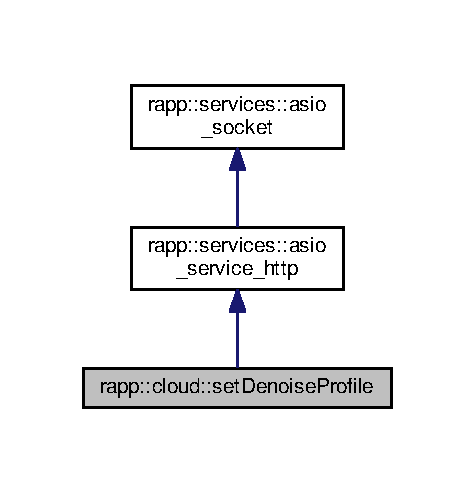
\includegraphics[width=228pt]{classrapp_1_1cloud_1_1setDenoiseProfile__inherit__graph}
\end{center}
\end{figure}


Collaboration diagram for rapp\-:\-:cloud\-:\-:set\-Denoise\-Profile\-:
\nopagebreak
\begin{figure}[H]
\begin{center}
\leavevmode
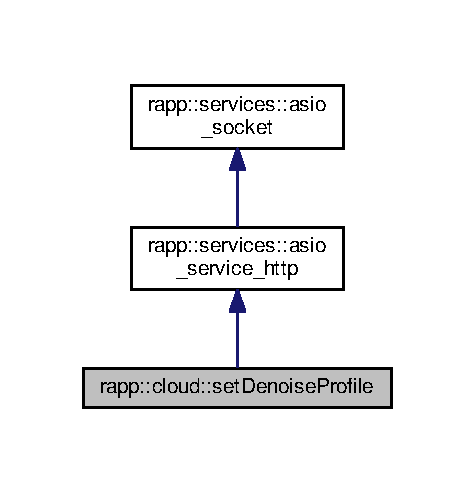
\includegraphics[width=228pt]{classrapp_1_1cloud_1_1setDenoiseProfile__coll__graph}
\end{center}
\end{figure}
\subsection*{Public Member Functions}
\begin{DoxyCompactItemize}
\item 
\hyperlink{classrapp_1_1cloud_1_1setDenoiseProfile_a2a4b101d2ff4b203cfc847b3cc69c50e}{set\-Denoise\-Profile} (const std\-::shared\-\_\-ptr$<$ \hyperlink{classrapp_1_1object_1_1audio}{rapp\-::object\-::audio} $>$ file, const std\-::string user, const std\-::string audio\-\_\-source)
\end{DoxyCompactItemize}
\subsection*{Private Member Functions}
\begin{DoxyCompactItemize}
\item 
void \hyperlink{classrapp_1_1cloud_1_1setDenoiseProfile_af30fee56946fd59af9bccce83a60d32a}{handle\-\_\-reply} (std\-::string json)
\end{DoxyCompactItemize}
\subsection*{Additional Inherited Members}


\subsection{Detailed Description}
setting the denoising audio profile for speech recognition 

\begin{DoxyVersion}{Version}
2 
\end{DoxyVersion}
\begin{DoxyDate}{Date}
20-\/\-September-\/2015 
\end{DoxyDate}
\begin{DoxyAuthor}{Author}
Alex Gkiokas \href{mailto:a.gkiokas@ortelio.co.uk}{\tt a.\-gkiokas@ortelio.\-co.\-uk} 
\end{DoxyAuthor}


Definition at line 13 of file set\-Denoise\-Profile.\-hpp.



\subsection{Constructor \& Destructor Documentation}
\hypertarget{classrapp_1_1cloud_1_1setDenoiseProfile_a2a4b101d2ff4b203cfc847b3cc69c50e}{\index{rapp\-::cloud\-::set\-Denoise\-Profile@{rapp\-::cloud\-::set\-Denoise\-Profile}!set\-Denoise\-Profile@{set\-Denoise\-Profile}}
\index{set\-Denoise\-Profile@{set\-Denoise\-Profile}!rapp::cloud::setDenoiseProfile@{rapp\-::cloud\-::set\-Denoise\-Profile}}
\subsubsection[{set\-Denoise\-Profile}]{\setlength{\rightskip}{0pt plus 5cm}rapp\-::cloud\-::set\-Denoise\-Profile\-::set\-Denoise\-Profile (
\begin{DoxyParamCaption}
\item[{const std\-::shared\-\_\-ptr$<$ {\bf rapp\-::object\-::audio} $>$}]{file, }
\item[{const std\-::string}]{user, }
\item[{const std\-::string}]{audio\-\_\-source}
\end{DoxyParamCaption}
)}}\label{classrapp_1_1cloud_1_1setDenoiseProfile_a2a4b101d2ff4b203cfc847b3cc69c50e}
This class does not return something, it only captures an error 

Definition at line 20 of file set\-Denoise\-Profile.\-hpp.



\subsection{Member Function Documentation}
\hypertarget{classrapp_1_1cloud_1_1setDenoiseProfile_af30fee56946fd59af9bccce83a60d32a}{\index{rapp\-::cloud\-::set\-Denoise\-Profile@{rapp\-::cloud\-::set\-Denoise\-Profile}!handle\-\_\-reply@{handle\-\_\-reply}}
\index{handle\-\_\-reply@{handle\-\_\-reply}!rapp::cloud::setDenoiseProfile@{rapp\-::cloud\-::set\-Denoise\-Profile}}
\subsubsection[{handle\-\_\-reply}]{\setlength{\rightskip}{0pt plus 5cm}void rapp\-::cloud\-::set\-Denoise\-Profile\-::handle\-\_\-reply (
\begin{DoxyParamCaption}
\item[{std\-::string}]{json}
\end{DoxyParamCaption}
)\hspace{0.3cm}{\ttfamily [private]}}}\label{classrapp_1_1cloud_1_1setDenoiseProfile_af30fee56946fd59af9bccce83a60d32a}


Definition at line 72 of file set\-Denoise\-Profile.\-hpp.



The documentation for this class was generated from the following file\-:\begin{DoxyCompactItemize}
\item 
/home/travis/rapp\-\_\-temp/rapp-\/api/cpp/includes/cloud/set\-Denoise\-Profile/\hyperlink{setDenoiseProfile_8hpp}{set\-Denoise\-Profile.\-hpp}\end{DoxyCompactItemize}

\hypertarget{classrapp_1_1cloud_1_1speechToText}{\section{rapp\-:\-:cloud\-:\-:speech\-To\-Text Class Reference}
\label{classrapp_1_1cloud_1_1speechToText}\index{rapp\-::cloud\-::speech\-To\-Text@{rapp\-::cloud\-::speech\-To\-Text}}
}


Asynchronous Service which will request the cloud to process speech-\/to-\/text.  




{\ttfamily \#include $<$speech\-To\-Text.\-hpp$>$}



Inheritance diagram for rapp\-:\-:cloud\-:\-:speech\-To\-Text\-:
\nopagebreak
\begin{figure}[H]
\begin{center}
\leavevmode
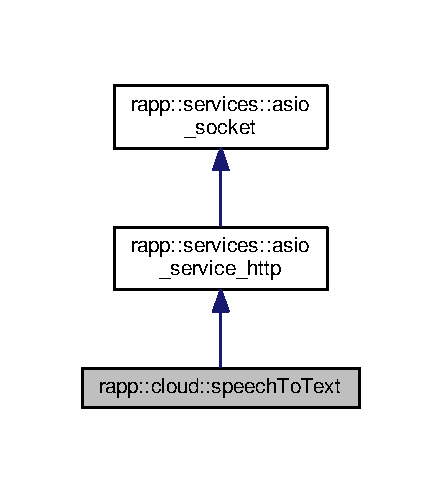
\includegraphics[width=212pt]{classrapp_1_1cloud_1_1speechToText__inherit__graph}
\end{center}
\end{figure}


Collaboration diagram for rapp\-:\-:cloud\-:\-:speech\-To\-Text\-:
\nopagebreak
\begin{figure}[H]
\begin{center}
\leavevmode
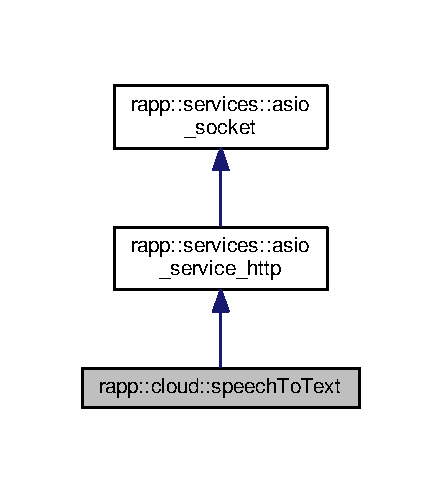
\includegraphics[width=212pt]{classrapp_1_1cloud_1_1speechToText__coll__graph}
\end{center}
\end{figure}
\subsection*{Public Member Functions}
\begin{DoxyCompactItemize}
\item 
\hyperlink{classrapp_1_1cloud_1_1speechToText_a4e9fe20b037d501cad760f854d6ebf3d}{speech\-To\-Text} (const std\-::shared\-\_\-ptr$<$ \hyperlink{classrapp_1_1object_1_1audio}{rapp\-::object\-::audio} $>$ file, const std\-::string language, const std\-::string user, const std\-::string audio\-\_\-source, const std\-::vector$<$ std\-::string $>$ grammar, const std\-::vector$<$ std\-::string $>$ words, const std\-::vector$<$ std\-::string $>$ sentences, std\-::function$<$ void(std\-::vector$<$ std\-::string $>$ words) $>$ callback)
\begin{DoxyCompactList}\small\item\em Contrusct a \hyperlink{classrapp_1_1cloud_1_1speechToText}{speech\-To\-Text} handler. \end{DoxyCompactList}\end{DoxyCompactItemize}
\subsection*{Private Member Functions}
\begin{DoxyCompactItemize}
\item 
void \hyperlink{classrapp_1_1cloud_1_1speechToText_aac8bc1b1fb840a53f904e6a20347e54d}{handle\-\_\-reply} (std\-::string json)
\end{DoxyCompactItemize}
\subsection*{Private Attributes}
\begin{DoxyCompactItemize}
\item 
std\-::function$<$ void(std\-::vector\\*
$<$ std\-::string $>$ words) $>$ \hyperlink{classrapp_1_1cloud_1_1speechToText_a2b06ddad67ab4600f2179b7b04c01b51}{delegate\-\_\-}
\begin{DoxyCompactList}\small\item\em The callback called upon completion of receiving the detected words. \end{DoxyCompactList}\end{DoxyCompactItemize}
\subsection*{Additional Inherited Members}


\subsection{Detailed Description}
Asynchronous Service which will request the cloud to process speech-\/to-\/text. 

\begin{DoxyVersion}{Version}
1 
\end{DoxyVersion}
\begin{DoxyDate}{Date}
19-\/\-September-\/2015 
\end{DoxyDate}
\begin{DoxyAuthor}{Author}
Alex Gkiokas \href{mailto:a.gkiokas@ortelio.co.uk}{\tt a.\-gkiokas@ortelio.\-co.\-uk} 
\end{DoxyAuthor}


Definition at line 13 of file speech\-To\-Text.\-hpp.



\subsection{Constructor \& Destructor Documentation}
\hypertarget{classrapp_1_1cloud_1_1speechToText_a4e9fe20b037d501cad760f854d6ebf3d}{\index{rapp\-::cloud\-::speech\-To\-Text@{rapp\-::cloud\-::speech\-To\-Text}!speech\-To\-Text@{speech\-To\-Text}}
\index{speech\-To\-Text@{speech\-To\-Text}!rapp::cloud::speechToText@{rapp\-::cloud\-::speech\-To\-Text}}
\subsubsection[{speech\-To\-Text}]{\setlength{\rightskip}{0pt plus 5cm}rapp\-::cloud\-::speech\-To\-Text\-::speech\-To\-Text (
\begin{DoxyParamCaption}
\item[{const std\-::shared\-\_\-ptr$<$ {\bf rapp\-::object\-::audio} $>$}]{file, }
\item[{const std\-::string}]{language, }
\item[{const std\-::string}]{user, }
\item[{const std\-::string}]{audio\-\_\-source, }
\item[{const std\-::vector$<$ std\-::string $>$}]{grammar, }
\item[{const std\-::vector$<$ std\-::string $>$}]{words, }
\item[{const std\-::vector$<$ std\-::string $>$}]{sentences, }
\item[{std\-::function$<$ void(std\-::vector$<$ std\-::string $>$ words) $>$}]{callback}
\end{DoxyParamCaption}
)}}\label{classrapp_1_1cloud_1_1speechToText_a4e9fe20b037d501cad760f854d6ebf3d}


Contrusct a \hyperlink{classrapp_1_1cloud_1_1speechToText}{speech\-To\-Text} handler. 


\begin{DoxyParams}{Parameters}
{\em audio} & is the actual binary sound file \\
\hline
{\em language} & is the language used for speech to text \\
\hline
{\em grammar} & is the Grammars used in Spc2\-Txt \\
\hline
{\em user} & is the user token \\
\hline
{\em words} & will be searched for in the audio \\
\hline
{\em sentences} & will be under consideration \\
\hline
{\em callback} & will be executed once the rapp cloud has responded \\
\hline
\end{DoxyParams}


Definition at line 27 of file speech\-To\-Text.\-hpp.



\subsection{Member Function Documentation}
\hypertarget{classrapp_1_1cloud_1_1speechToText_aac8bc1b1fb840a53f904e6a20347e54d}{\index{rapp\-::cloud\-::speech\-To\-Text@{rapp\-::cloud\-::speech\-To\-Text}!handle\-\_\-reply@{handle\-\_\-reply}}
\index{handle\-\_\-reply@{handle\-\_\-reply}!rapp::cloud::speechToText@{rapp\-::cloud\-::speech\-To\-Text}}
\subsubsection[{handle\-\_\-reply}]{\setlength{\rightskip}{0pt plus 5cm}void rapp\-::cloud\-::speech\-To\-Text\-::handle\-\_\-reply (
\begin{DoxyParamCaption}
\item[{std\-::string}]{json}
\end{DoxyParamCaption}
)\hspace{0.3cm}{\ttfamily [private]}}}\label{classrapp_1_1cloud_1_1speechToText_aac8bc1b1fb840a53f904e6a20347e54d}


Definition at line 117 of file speech\-To\-Text.\-hpp.



\subsection{Member Data Documentation}
\hypertarget{classrapp_1_1cloud_1_1speechToText_a2b06ddad67ab4600f2179b7b04c01b51}{\index{rapp\-::cloud\-::speech\-To\-Text@{rapp\-::cloud\-::speech\-To\-Text}!delegate\-\_\-@{delegate\-\_\-}}
\index{delegate\-\_\-@{delegate\-\_\-}!rapp::cloud::speechToText@{rapp\-::cloud\-::speech\-To\-Text}}
\subsubsection[{delegate\-\_\-}]{\setlength{\rightskip}{0pt plus 5cm}std\-::function$<$ void( std\-::vector$<$std\-::string$>$ words ) $>$ rapp\-::cloud\-::speech\-To\-Text\-::delegate\-\_\-\hspace{0.3cm}{\ttfamily [private]}}}\label{classrapp_1_1cloud_1_1speechToText_a2b06ddad67ab4600f2179b7b04c01b51}


The callback called upon completion of receiving the detected words. 



Definition at line 151 of file speech\-To\-Text.\-hpp.



The documentation for this class was generated from the following file\-:\begin{DoxyCompactItemize}
\item 
/home/travis/rapp\-\_\-temp/rapp-\/api/cpp/includes/cloud/speech\-To\-Text/\hyperlink{speechToText_8hpp}{speech\-To\-Text.\-hpp}\end{DoxyCompactItemize}

\hypertarget{classrapp_1_1robot_1_1vision}{\section{rapp\-:\-:robot\-:\-:vision Class Reference}
\label{classrapp_1_1robot_1_1vision}\index{rapp\-::robot\-::vision@{rapp\-::robot\-::vision}}
}


Abstract Base Class (A\-B\-C) Interface for Vision.  




{\ttfamily \#include $<$vision.\-hpp$>$}



Inheritance diagram for rapp\-:\-:robot\-:\-:vision\-:
\nopagebreak
\begin{figure}[H]
\begin{center}
\leavevmode
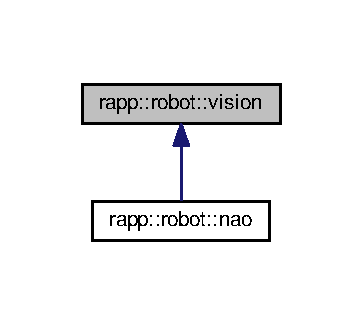
\includegraphics[width=174pt]{classrapp_1_1robot_1_1vision__inherit__graph}
\end{center}
\end{figure}
\subsection*{Public Member Functions}
\begin{DoxyCompactItemize}
\item 
virtual std\-::shared\-\_\-pointr\\*
$<$ \hyperlink{classrapp_1_1object_1_1picture}{rapp\-::object\-::picture} $>$ \hyperlink{classrapp_1_1robot_1_1vision_ac6f224f2da0d9512b8c6700de3eded85}{capture\-Image} (std\-::string camera\-Id, int camera\-Resolution) const =0
\begin{DoxyCompactList}\small\item\em N\-O\-T\-E\-: What about format? \end{DoxyCompactList}\end{DoxyCompactItemize}


\subsection{Detailed Description}
Abstract Base Class (A\-B\-C) Interface for Vision. 

\begin{DoxyVersion}{Version}
1 
\end{DoxyVersion}
\begin{DoxyDate}{Date}
20-\/\-September-\/2015 
\end{DoxyDate}
\begin{DoxyAuthor}{Author}
Alex Gkiokas \href{mailto:a.gkiokas@ortelio.co.uk}{\tt a.\-gkiokas@ortelio.\-co.\-uk} 
\end{DoxyAuthor}


Definition at line 13 of file vision.\-hpp.



\subsection{Member Function Documentation}
\hypertarget{classrapp_1_1robot_1_1vision_ac6f224f2da0d9512b8c6700de3eded85}{\index{rapp\-::robot\-::vision@{rapp\-::robot\-::vision}!capture\-Image@{capture\-Image}}
\index{capture\-Image@{capture\-Image}!rapp::robot::vision@{rapp\-::robot\-::vision}}
\subsubsection[{capture\-Image}]{\setlength{\rightskip}{0pt plus 5cm}virtual std\-::shared\-\_\-pointr$<${\bf rapp\-::object\-::picture}$>$ rapp\-::robot\-::vision\-::capture\-Image (
\begin{DoxyParamCaption}
\item[{std\-::string}]{camera\-Id, }
\item[{int}]{camera\-Resolution}
\end{DoxyParamCaption}
) const\hspace{0.3cm}{\ttfamily [pure virtual]}}}\label{classrapp_1_1robot_1_1vision_ac6f224f2da0d9512b8c6700de3eded85}


N\-O\-T\-E\-: What about format? 



Implemented in \hyperlink{classrapp_1_1robot_1_1nao_a276172d720ce8387a3fe695e02753af0}{rapp\-::robot\-::nao}.



The documentation for this class was generated from the following file\-:\begin{DoxyCompactItemize}
\item 
/home/travis/rapp\-\_\-temp/rapp-\/api/cpp/includes/robot/vision/\hyperlink{vision_8hpp}{vision.\-hpp}\end{DoxyCompactItemize}

\chapter{File Documentation}
\hypertarget{face__detect_8cpp}{\section{/home/travis/rapp\-\_\-temp/rapp-\/api/cpp/examples/face\-\_\-detect.cpp File Reference}
\label{face__detect_8cpp}\index{/home/travis/rapp\-\_\-temp/rapp-\/api/cpp/examples/face\-\_\-detect.\-cpp@{/home/travis/rapp\-\_\-temp/rapp-\/api/cpp/examples/face\-\_\-detect.\-cpp}}
}
{\ttfamily \#include \char`\"{}cloud/service\-\_\-controller/service\-\_\-controller.\-hpp\char`\"{}}\\*
{\ttfamily \#include \char`\"{}cloud/vision/face\-\_\-detection/face\-\_\-detection.\-hpp\char`\"{}}\\*
{\ttfamily \#include \char`\"{}objects/picture/picture.\-hpp\char`\"{}}\\*
Include dependency graph for face\-\_\-detect.\-cpp\-:
\nopagebreak
\begin{figure}[H]
\begin{center}
\leavevmode
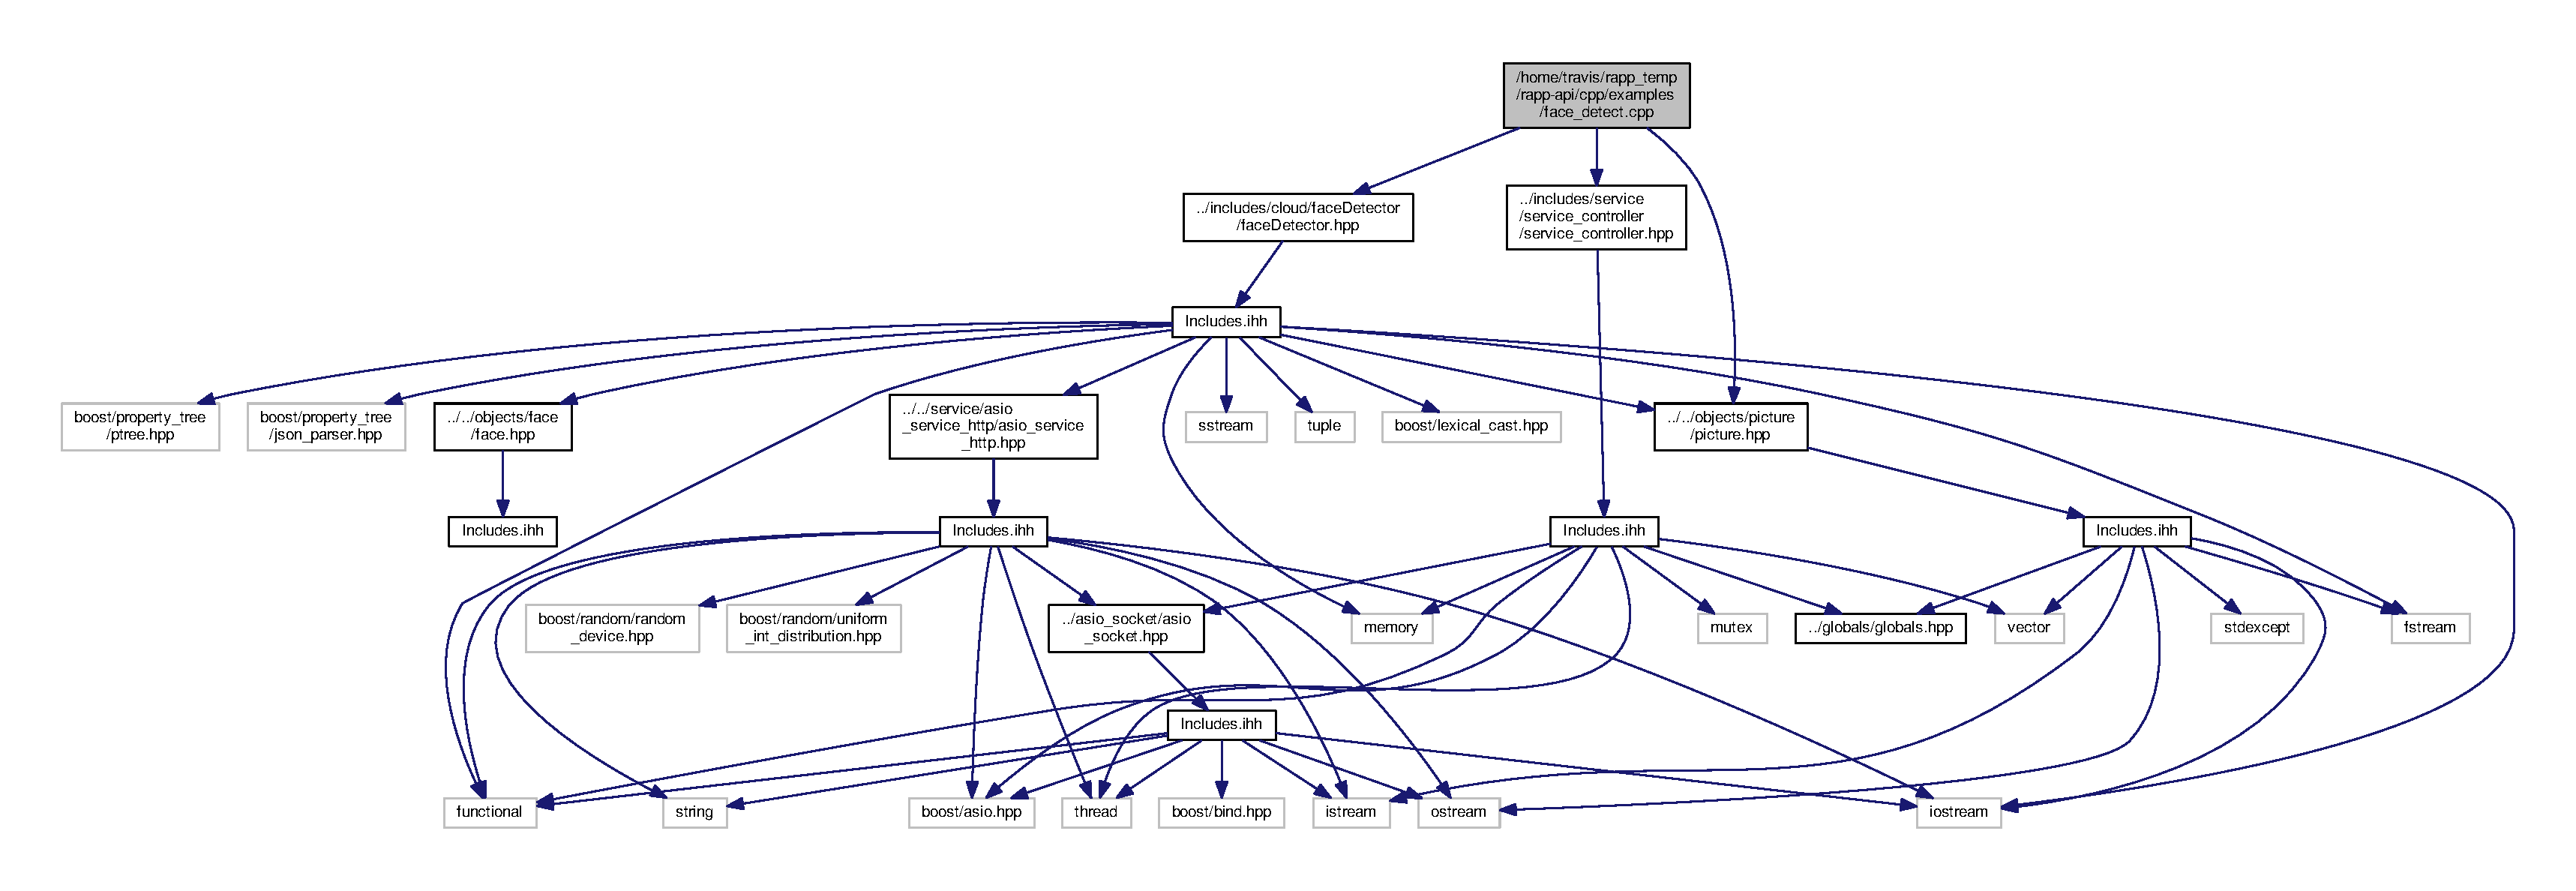
\includegraphics[width=350pt]{face__detect_8cpp__incl}
\end{center}
\end{figure}
\subsection*{Functions}
\begin{DoxyCompactItemize}
\item 
int \hyperlink{face__detect_8cpp_a0ddf1224851353fc92bfbff6f499fa97}{main} (int argc, char $\ast$argv\mbox{[}$\,$\mbox{]})
\end{DoxyCompactItemize}


\subsection{Function Documentation}
\hypertarget{face__detect_8cpp_a0ddf1224851353fc92bfbff6f499fa97}{\index{face\-\_\-detect.\-cpp@{face\-\_\-detect.\-cpp}!main@{main}}
\index{main@{main}!face_detect.cpp@{face\-\_\-detect.\-cpp}}
\subsubsection[{main}]{\setlength{\rightskip}{0pt plus 5cm}int main (
\begin{DoxyParamCaption}
\item[{int}]{argc, }
\item[{char $\ast$}]{argv\mbox{[}$\,$\mbox{]}}
\end{DoxyParamCaption}
)}}\label{face__detect_8cpp_a0ddf1224851353fc92bfbff6f499fa97}
Pass as param a P\-N\-G image 

Definition at line 7 of file face\-\_\-detect.\-cpp.


\hypertarget{fetch__data_8cpp}{\section{/home/travis/rapp\-\_\-temp/rapp-\/api/cpp/examples/fetch\-\_\-data.cpp File Reference}
\label{fetch__data_8cpp}\index{/home/travis/rapp\-\_\-temp/rapp-\/api/cpp/examples/fetch\-\_\-data.\-cpp@{/home/travis/rapp\-\_\-temp/rapp-\/api/cpp/examples/fetch\-\_\-data.\-cpp}}
}

\hypertarget{ontology__example_8cpp}{\section{/home/travis/rapp\-\_\-temp/rapp-\/api/cpp/examples/ontology\-\_\-example.cpp File Reference}
\label{ontology__example_8cpp}\index{/home/travis/rapp\-\_\-temp/rapp-\/api/cpp/examples/ontology\-\_\-example.\-cpp@{/home/travis/rapp\-\_\-temp/rapp-\/api/cpp/examples/ontology\-\_\-example.\-cpp}}
}
{\ttfamily \#include \char`\"{}../includes/service/service\-\_\-controller/service\-\_\-controller.\-hpp\char`\"{}}\\*
{\ttfamily \#include \char`\"{}../includes/cloud/ontology\-Sub\-Classes\-Of/ontology\-Sub\-Classes\-Of.\-hpp\char`\"{}}\\*
{\ttfamily \#include \char`\"{}../includes/cloud/ontology\-Super\-Classes\-Of/ontology\-Super\-Classes\-Of.\-hpp\char`\"{}}\\*
{\ttfamily \#include \char`\"{}../includes/cloud/ontology\-Is\-Sub\-Super\-Class\-Of/ontology\-Is\-Sub\-Super\-Class\-Of.\-hpp\char`\"{}}\\*
{\ttfamily \#include $<$iostream$>$}\\*
Include dependency graph for ontology\-\_\-example.\-cpp\-:
\nopagebreak
\begin{figure}[H]
\begin{center}
\leavevmode
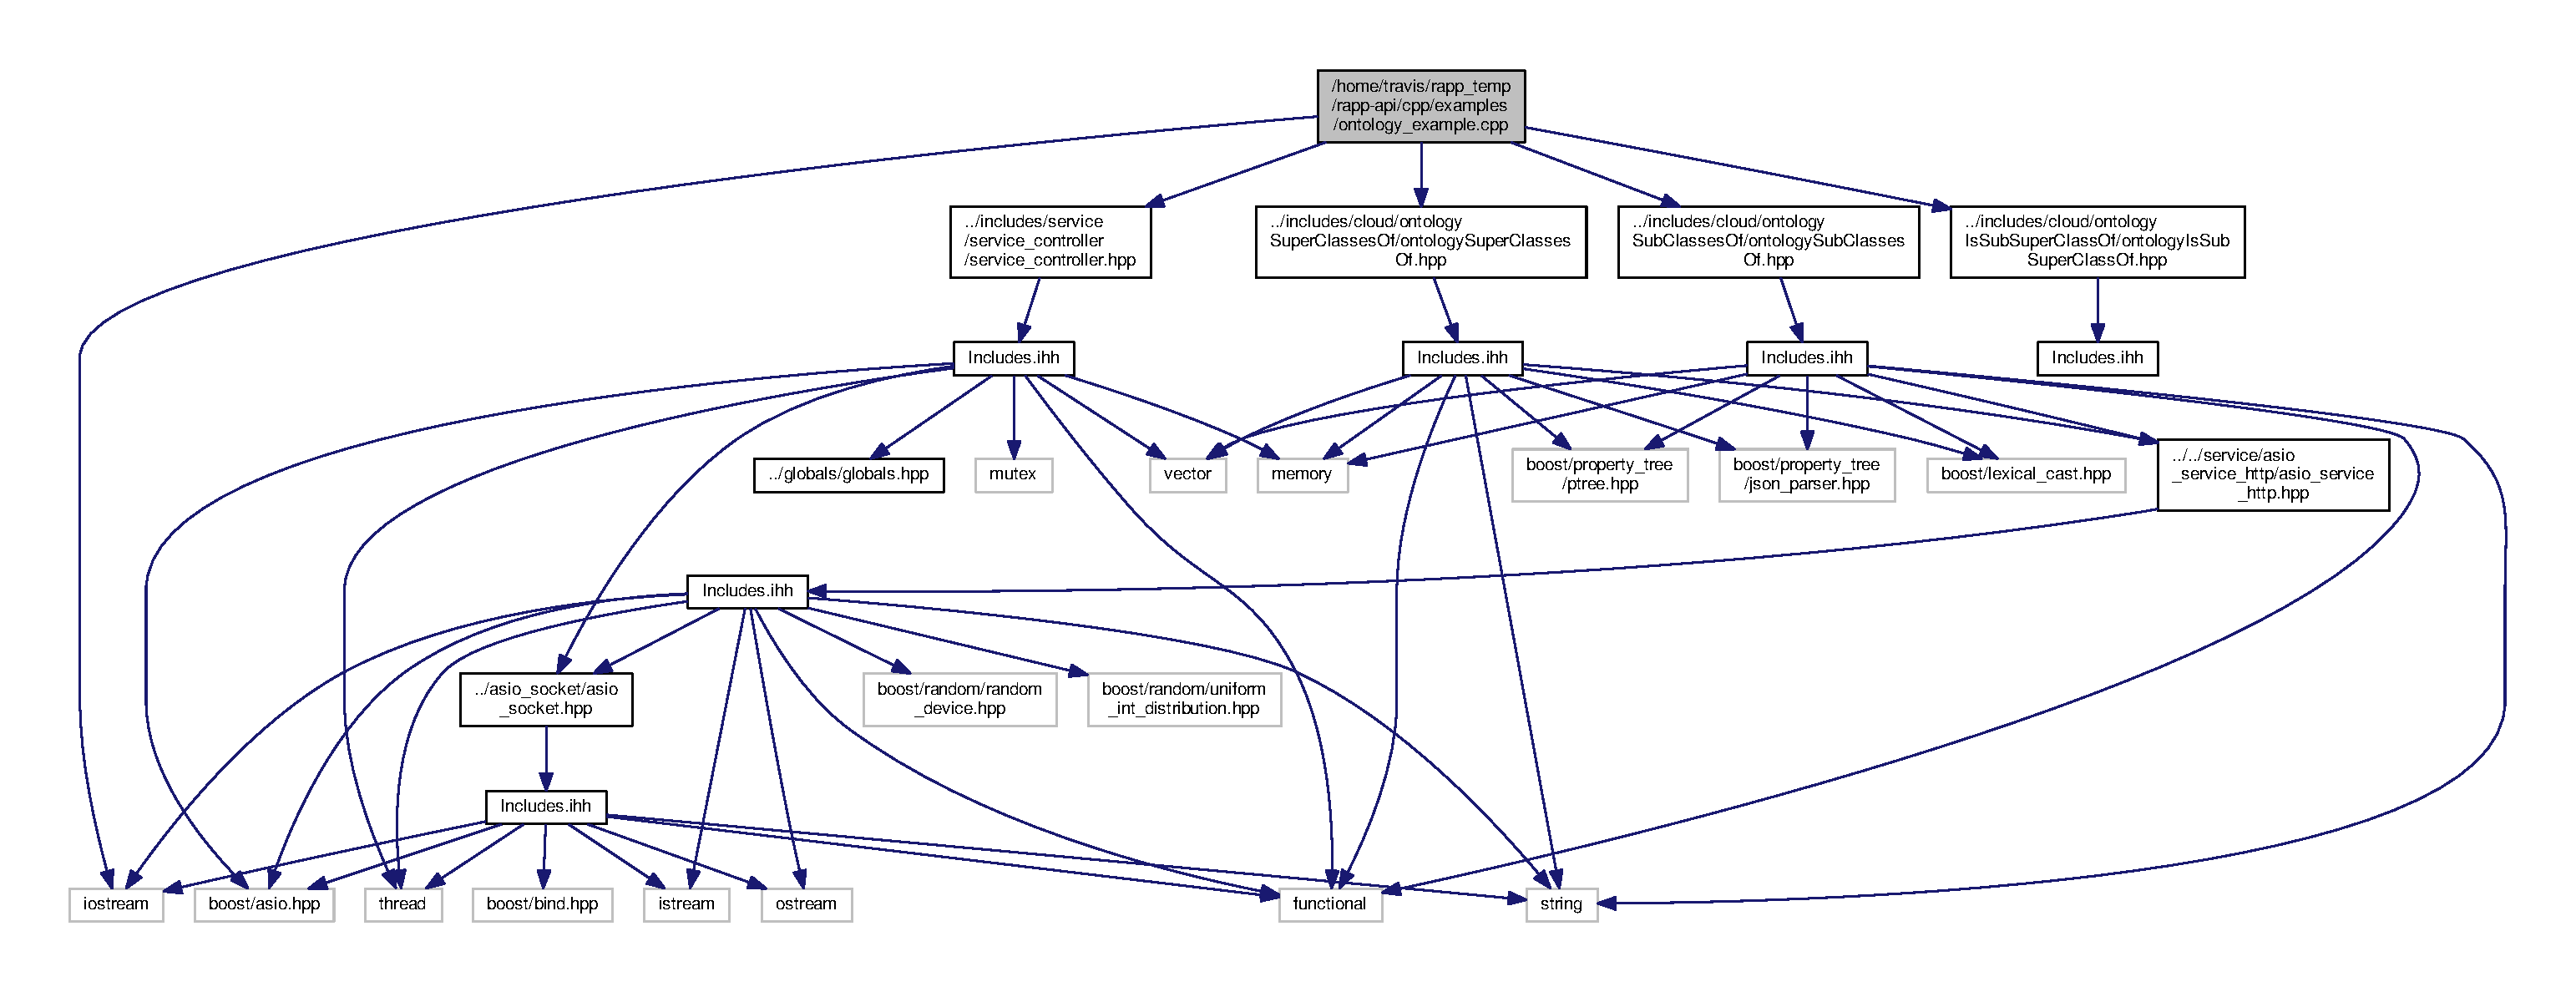
\includegraphics[width=350pt]{ontology__example_8cpp__incl}
\end{center}
\end{figure}
\subsection*{Functions}
\begin{DoxyCompactItemize}
\item 
int \hyperlink{ontology__example_8cpp_a0ddf1224851353fc92bfbff6f499fa97}{main} (int argc, char $\ast$argv\mbox{[}$\,$\mbox{]})
\end{DoxyCompactItemize}


\subsection{Function Documentation}
\hypertarget{ontology__example_8cpp_a0ddf1224851353fc92bfbff6f499fa97}{\index{ontology\-\_\-example.\-cpp@{ontology\-\_\-example.\-cpp}!main@{main}}
\index{main@{main}!ontology_example.cpp@{ontology\-\_\-example.\-cpp}}
\subsubsection[{main}]{\setlength{\rightskip}{0pt plus 5cm}int main (
\begin{DoxyParamCaption}
\item[{int}]{argc, }
\item[{char $\ast$}]{argv\mbox{[}$\,$\mbox{]}}
\end{DoxyParamCaption}
)}}\label{ontology__example_8cpp_a0ddf1224851353fc92bfbff6f499fa97}


Definition at line 7 of file ontology\-\_\-example.\-cpp.


\hypertarget{picture__example_8cpp}{\section{/home/travis/rapp\-\_\-temp/rapp-\/api/cpp/examples/picture\-\_\-example.cpp File Reference}
\label{picture__example_8cpp}\index{/home/travis/rapp\-\_\-temp/rapp-\/api/cpp/examples/picture\-\_\-example.\-cpp@{/home/travis/rapp\-\_\-temp/rapp-\/api/cpp/examples/picture\-\_\-example.\-cpp}}
}
{\ttfamily \#include \char`\"{}objects/picture/picture.\-hpp\char`\"{}}\\*
{\ttfamily \#include $<$memory$>$}\\*
Include dependency graph for picture\-\_\-example.\-cpp\-:
\nopagebreak
\begin{figure}[H]
\begin{center}
\leavevmode
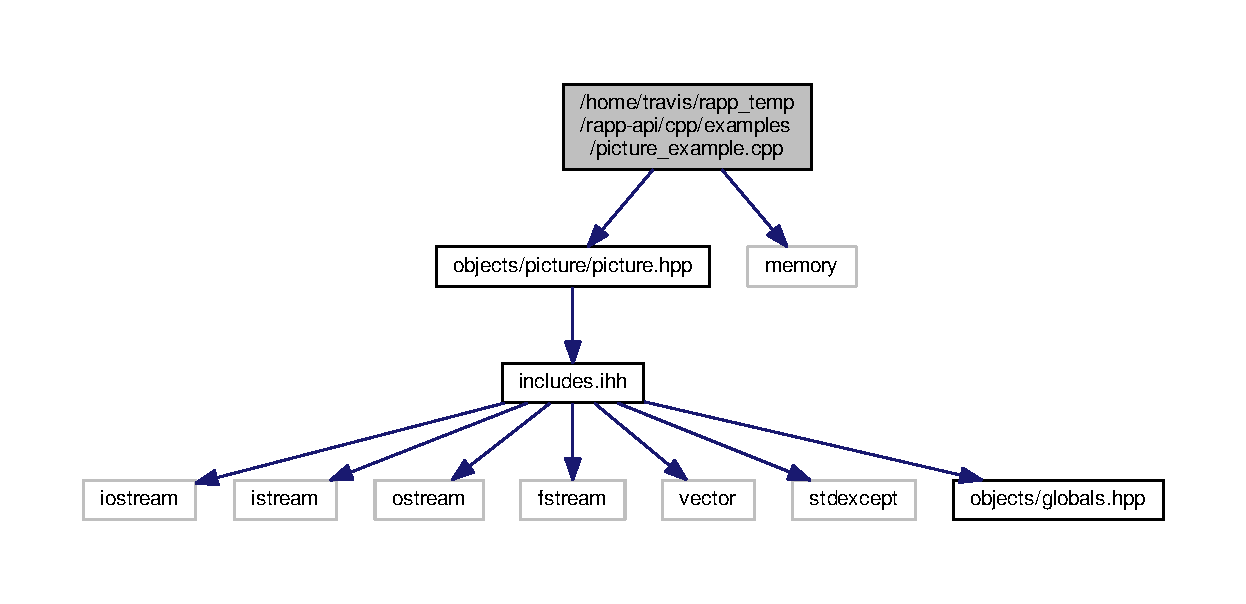
\includegraphics[width=350pt]{picture__example_8cpp__incl}
\end{center}
\end{figure}
\subsection*{Functions}
\begin{DoxyCompactItemize}
\item 
int \hyperlink{picture__example_8cpp_a0ddf1224851353fc92bfbff6f499fa97}{main} (int argc, char $\ast$argv\mbox{[}$\,$\mbox{]})
\end{DoxyCompactItemize}


\subsection{Function Documentation}
\hypertarget{picture__example_8cpp_a0ddf1224851353fc92bfbff6f499fa97}{\index{picture\-\_\-example.\-cpp@{picture\-\_\-example.\-cpp}!main@{main}}
\index{main@{main}!picture_example.cpp@{picture\-\_\-example.\-cpp}}
\subsubsection[{main}]{\setlength{\rightskip}{0pt plus 5cm}int main (
\begin{DoxyParamCaption}
\item[{int}]{argc, }
\item[{char $\ast$}]{argv\mbox{[}$\,$\mbox{]}}
\end{DoxyParamCaption}
)}}\label{picture__example_8cpp_a0ddf1224851353fc92bfbff6f499fa97}
Open a picture and load it into an object 

Definition at line 6 of file picture\-\_\-example.\-cpp.


\hypertarget{qr__detect_8cpp}{\section{/home/travis/rapp\-\_\-temp/rapp-\/api/cpp/examples/qr\-\_\-detect.cpp File Reference}
\label{qr__detect_8cpp}\index{/home/travis/rapp\-\_\-temp/rapp-\/api/cpp/examples/qr\-\_\-detect.\-cpp@{/home/travis/rapp\-\_\-temp/rapp-\/api/cpp/examples/qr\-\_\-detect.\-cpp}}
}
{\ttfamily \#include \char`\"{}cloud/service\-\_\-controller/service\-\_\-controller.\-hpp\char`\"{}}\\*
{\ttfamily \#include \char`\"{}cloud/vision/qr\-\_\-detection/qr\-\_\-detection.\-hpp\char`\"{}}\\*
{\ttfamily \#include \char`\"{}objects/picture/picture.\-hpp\char`\"{}}\\*
Include dependency graph for qr\-\_\-detect.\-cpp\-:
\nopagebreak
\begin{figure}[H]
\begin{center}
\leavevmode
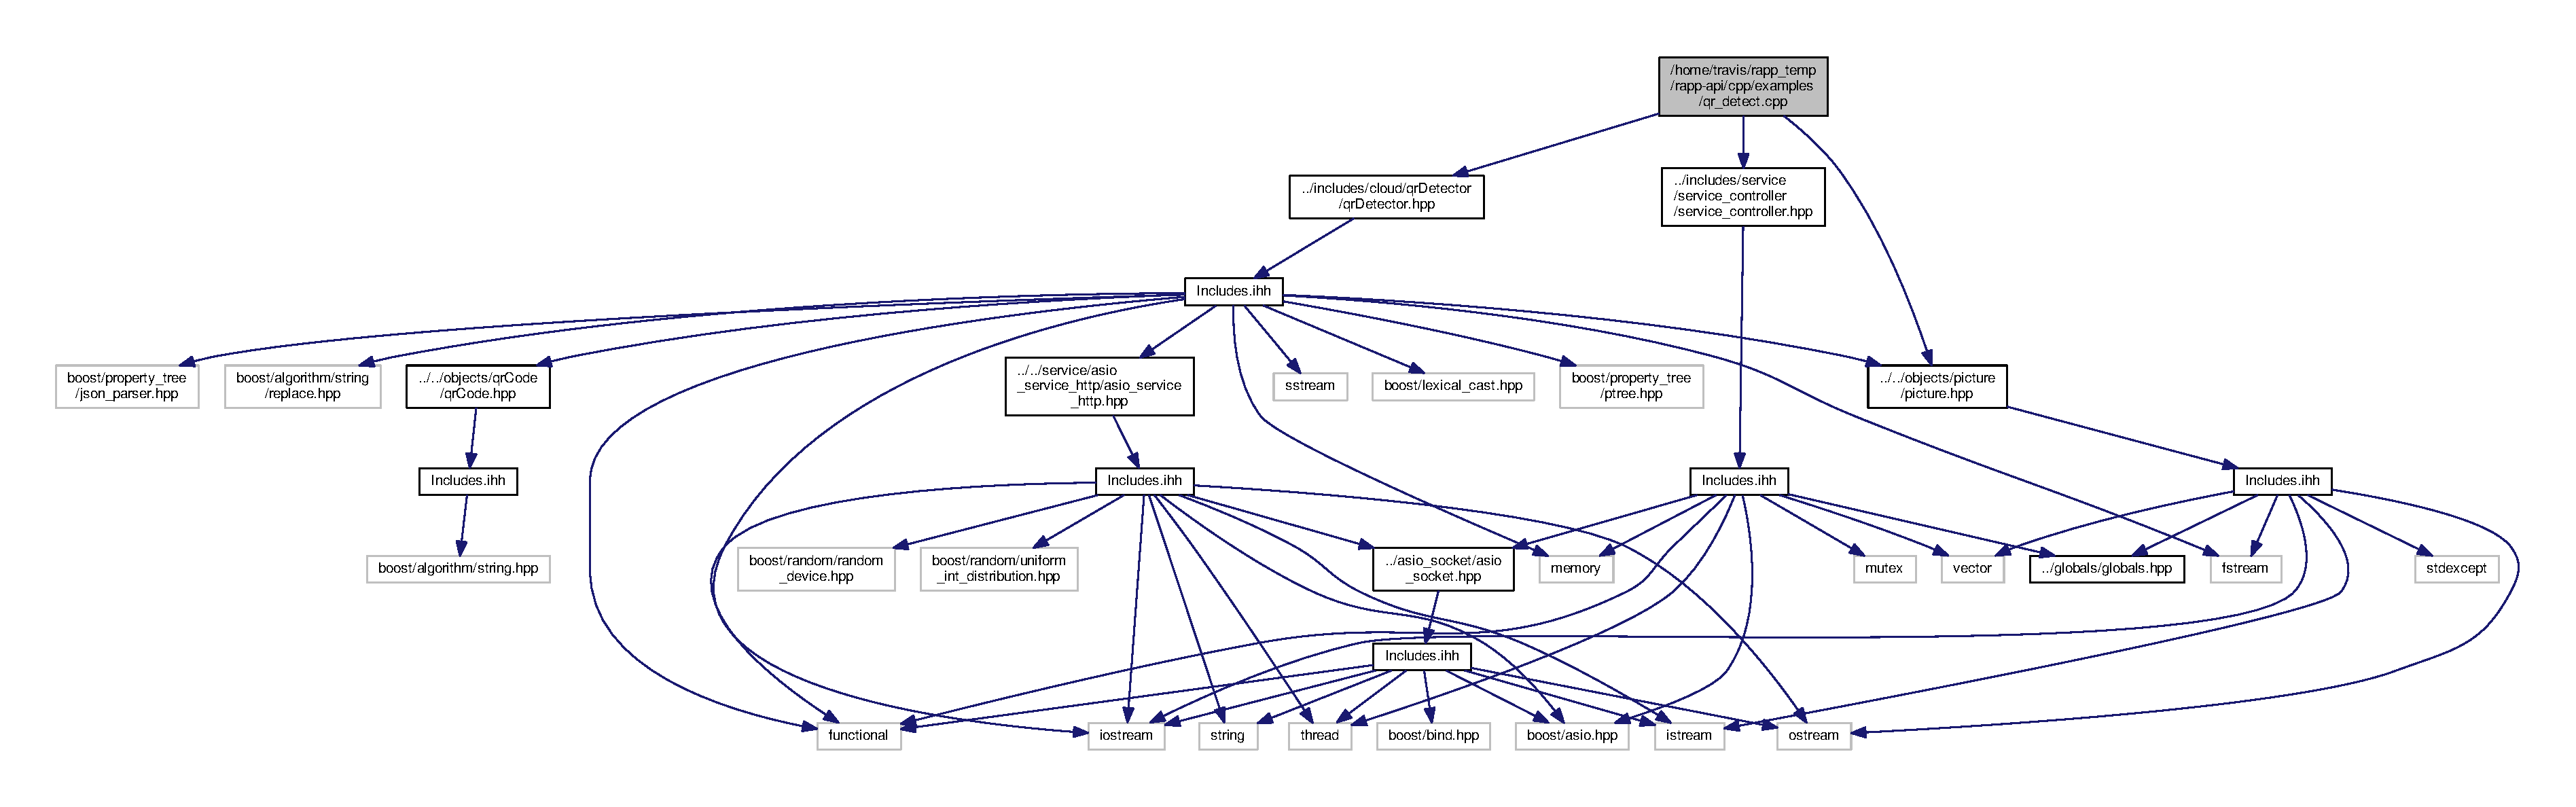
\includegraphics[width=350pt]{qr__detect_8cpp__incl}
\end{center}
\end{figure}
\subsection*{Functions}
\begin{DoxyCompactItemize}
\item 
int \hyperlink{qr__detect_8cpp_a0ddf1224851353fc92bfbff6f499fa97}{main} (int argc, char $\ast$argv\mbox{[}$\,$\mbox{]})
\end{DoxyCompactItemize}


\subsection{Function Documentation}
\hypertarget{qr__detect_8cpp_a0ddf1224851353fc92bfbff6f499fa97}{\index{qr\-\_\-detect.\-cpp@{qr\-\_\-detect.\-cpp}!main@{main}}
\index{main@{main}!qr_detect.cpp@{qr\-\_\-detect.\-cpp}}
\subsubsection[{main}]{\setlength{\rightskip}{0pt plus 5cm}int main (
\begin{DoxyParamCaption}
\item[{int}]{argc, }
\item[{char $\ast$}]{argv\mbox{[}$\,$\mbox{]}}
\end{DoxyParamCaption}
)}}\label{qr__detect_8cpp_a0ddf1224851353fc92bfbff6f499fa97}
Pass as argv\mbox{[}1\mbox{]} an image with a Q\-R code 

Definition at line 7 of file qr\-\_\-detect.\-cpp.


\hypertarget{set__denoise__example_8cpp}{\section{/home/travis/rapp\-\_\-temp/rapp-\/api/cpp/examples/set\-\_\-denoise\-\_\-example.cpp File Reference}
\label{set__denoise__example_8cpp}\index{/home/travis/rapp\-\_\-temp/rapp-\/api/cpp/examples/set\-\_\-denoise\-\_\-example.\-cpp@{/home/travis/rapp\-\_\-temp/rapp-\/api/cpp/examples/set\-\_\-denoise\-\_\-example.\-cpp}}
}
{\ttfamily \#include \char`\"{}../includes/service/service\-\_\-controller/service\-\_\-controller.\-hpp\char`\"{}}\\*
{\ttfamily \#include \char`\"{}../includes/cloud/set\-Denoise\-Profile/set\-Denoise\-Profile.\-hpp\char`\"{}}\\*
{\ttfamily \#include \char`\"{}../includes/objects/audio/audio.\-hpp\char`\"{}}\\*
Include dependency graph for set\-\_\-denoise\-\_\-example.\-cpp\-:
\nopagebreak
\begin{figure}[H]
\begin{center}
\leavevmode
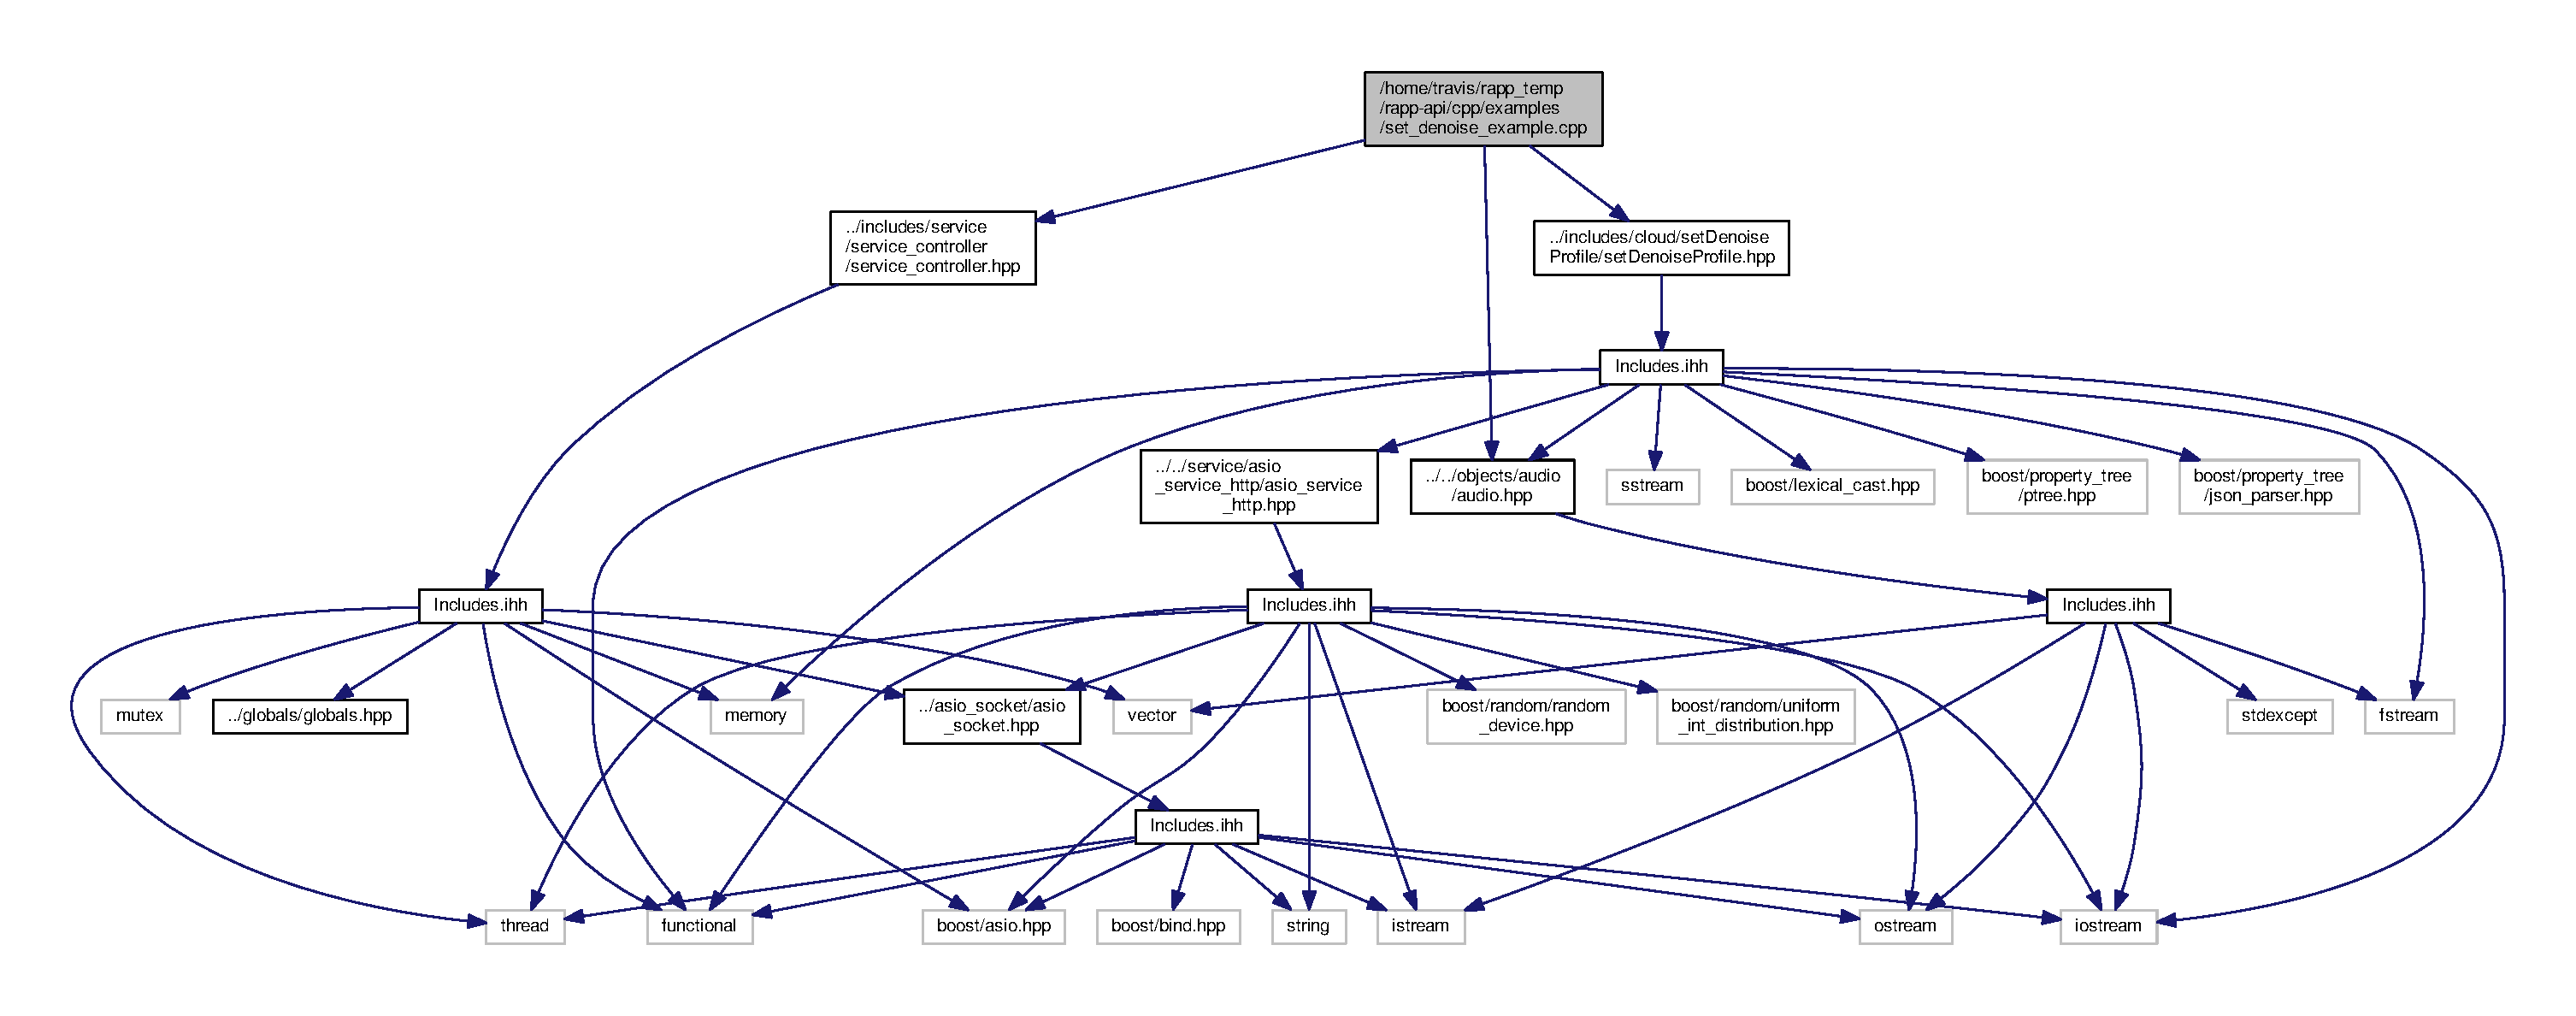
\includegraphics[width=350pt]{set__denoise__example_8cpp__incl}
\end{center}
\end{figure}
\subsection*{Functions}
\begin{DoxyCompactItemize}
\item 
int \hyperlink{set__denoise__example_8cpp_ae66f6b31b5ad750f1fe042a706a4e3d4}{main} ()
\end{DoxyCompactItemize}


\subsection{Function Documentation}
\hypertarget{set__denoise__example_8cpp_ae66f6b31b5ad750f1fe042a706a4e3d4}{\index{set\-\_\-denoise\-\_\-example.\-cpp@{set\-\_\-denoise\-\_\-example.\-cpp}!main@{main}}
\index{main@{main}!set_denoise_example.cpp@{set\-\_\-denoise\-\_\-example.\-cpp}}
\subsubsection[{main}]{\setlength{\rightskip}{0pt plus 5cm}int main (
\begin{DoxyParamCaption}
{}
\end{DoxyParamCaption}
)}}\label{set__denoise__example_8cpp_ae66f6b31b5ad750f1fe042a706a4e3d4}


Definition at line 5 of file set\-\_\-denoise\-\_\-example.\-cpp.


\hypertarget{speech__to__text_8cpp}{\section{/home/travis/rapp\-\_\-temp/rapp-\/api/cpp/examples/speech\-\_\-to\-\_\-text.cpp File Reference}
\label{speech__to__text_8cpp}\index{/home/travis/rapp\-\_\-temp/rapp-\/api/cpp/examples/speech\-\_\-to\-\_\-text.\-cpp@{/home/travis/rapp\-\_\-temp/rapp-\/api/cpp/examples/speech\-\_\-to\-\_\-text.\-cpp}}
}
{\ttfamily \#include \char`\"{}cloud/service\-\_\-controller/service\-\_\-controller.\-hpp\char`\"{}}\\*
{\ttfamily \#include \char`\"{}cloud/speech/speech\-\_\-detection\-\_\-sphinx4/speech\-\_\-detection\-\_\-sphinx4.\-hpp\char`\"{}}\\*
{\ttfamily \#include \char`\"{}objects/audio/audio.\-hpp\char`\"{}}\\*
{\ttfamily \#include $<$boost/program\-\_\-options.\-hpp$>$}\\*
{\ttfamily \#include $<$string$>$}\\*
{\ttfamily \#include $<$fstream$>$}\\*
{\ttfamily \#include $<$streambuf$>$}\\*
Include dependency graph for speech\-\_\-to\-\_\-text.\-cpp\-:
\nopagebreak
\begin{figure}[H]
\begin{center}
\leavevmode
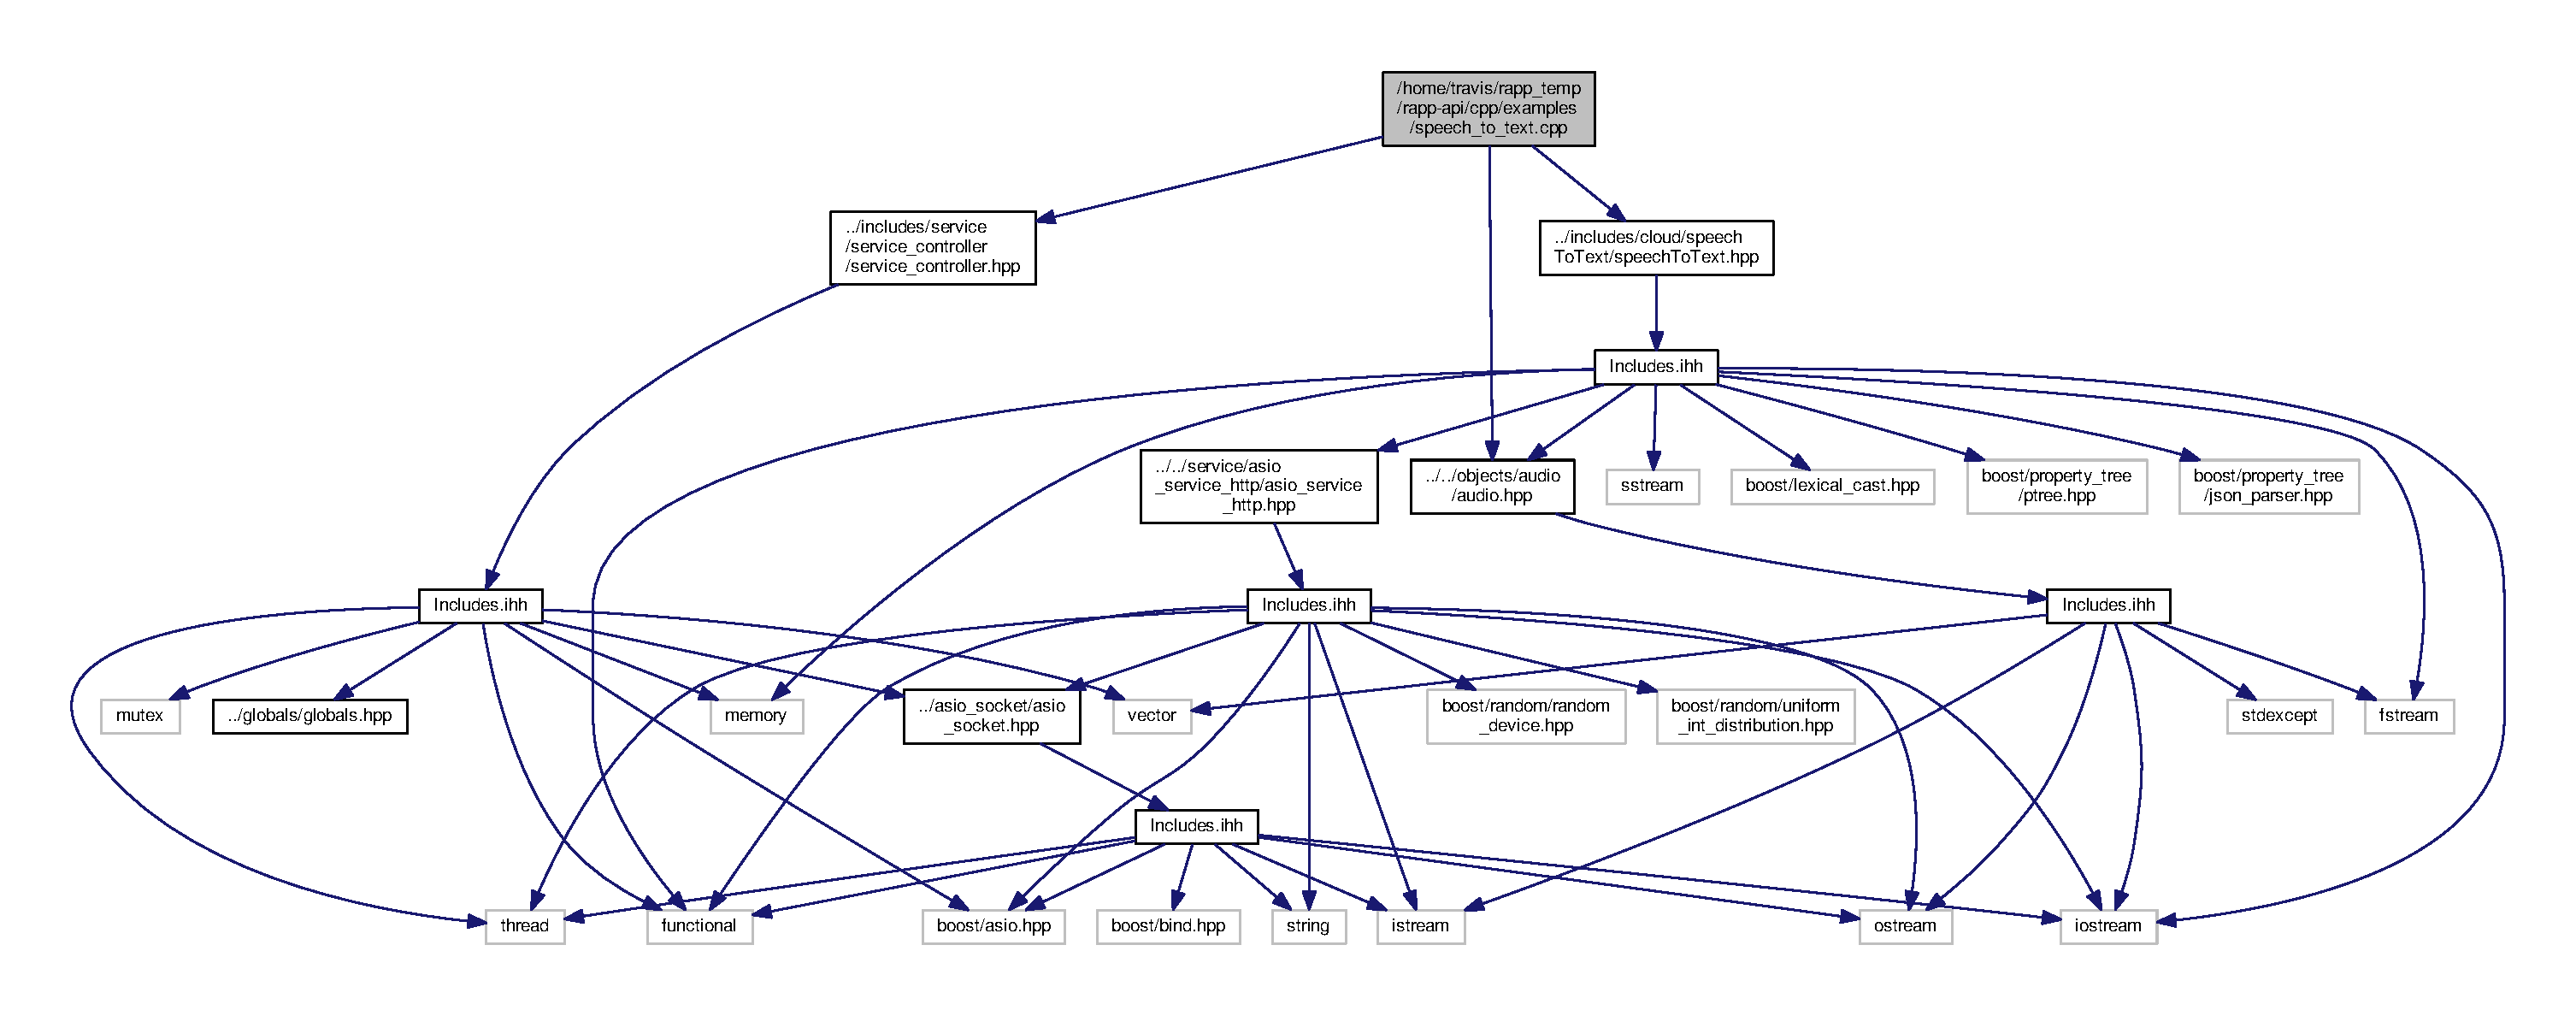
\includegraphics[width=350pt]{speech__to__text_8cpp__incl}
\end{center}
\end{figure}
\subsection*{Functions}
\begin{DoxyCompactItemize}
\item 
std\-::string \hyperlink{speech__to__text_8cpp_a597be07572d7933e8427bed8e833a86f}{load\-\_\-jsgf} (const std\-::string filename)
\item 
int \hyperlink{speech__to__text_8cpp_a0ddf1224851353fc92bfbff6f499fa97}{main} (int argc, char $\ast$argv\mbox{[}$\,$\mbox{]})
\item 
{\footnotesize template$<$class T $>$ }\\std\-::ostream \& \hyperlink{speech__to__text_8cpp_a4b8db62a17e01a839e499a4c59112df5}{operator$<$$<$} (std\-::ostream \&os, const std\-::vector$<$ T $>$ \&v)
\end{DoxyCompactItemize}


\subsection{Function Documentation}
\hypertarget{speech__to__text_8cpp_a597be07572d7933e8427bed8e833a86f}{\index{speech\-\_\-to\-\_\-text.\-cpp@{speech\-\_\-to\-\_\-text.\-cpp}!load\-\_\-jsgf@{load\-\_\-jsgf}}
\index{load\-\_\-jsgf@{load\-\_\-jsgf}!speech_to_text.cpp@{speech\-\_\-to\-\_\-text.\-cpp}}
\subsubsection[{load\-\_\-jsgf}]{\setlength{\rightskip}{0pt plus 5cm}std\-::string load\-\_\-jsgf (
\begin{DoxyParamCaption}
\item[{const std\-::string}]{filename}
\end{DoxyParamCaption}
)}}\label{speech__to__text_8cpp_a597be07572d7933e8427bed8e833a86f}


Definition at line 20 of file speech\-\_\-to\-\_\-text.\-cpp.

\hypertarget{speech__to__text_8cpp_a0ddf1224851353fc92bfbff6f499fa97}{\index{speech\-\_\-to\-\_\-text.\-cpp@{speech\-\_\-to\-\_\-text.\-cpp}!main@{main}}
\index{main@{main}!speech_to_text.cpp@{speech\-\_\-to\-\_\-text.\-cpp}}
\subsubsection[{main}]{\setlength{\rightskip}{0pt plus 5cm}int main (
\begin{DoxyParamCaption}
\item[{int}]{argc, }
\item[{char $\ast$}]{argv\mbox{[}$\,$\mbox{]}}
\end{DoxyParamCaption}
)}}\label{speech__to__text_8cpp_a0ddf1224851353fc92bfbff6f499fa97}
Query the C\-M\-U Sphinx4 engine for keywords and sentences using a W\-A\-V file argv\mbox{[}1\mbox{]}\-: audio file argv\mbox{[}2\mbox{]}\-: audio source type argv\mbox{[}3\mbox{]}\-: language argv\mbox{[}4\mbox{]}\-: user argv\mbox{[}5\mbox{]}\-: words to search for -\/ O\-P\-T\-I\-O\-N\-A\-L argv\mbox{[}6\mbox{]}\-: sentences to search for -\/ O\-P\-T\-I\-O\-N\-A\-L argv\mbox{[}7\mbox{]}\-: grammar file (J\-S\-G\-F text file) -\/ O\-P\-T\-I\-O\-N\-A\-L 

Definition at line 44 of file speech\-\_\-to\-\_\-text.\-cpp.

\hypertarget{speech__to__text_8cpp_a4b8db62a17e01a839e499a4c59112df5}{\index{speech\-\_\-to\-\_\-text.\-cpp@{speech\-\_\-to\-\_\-text.\-cpp}!operator$<$$<$@{operator$<$$<$}}
\index{operator$<$$<$@{operator$<$$<$}!speech_to_text.cpp@{speech\-\_\-to\-\_\-text.\-cpp}}
\subsubsection[{operator$<$$<$}]{\setlength{\rightskip}{0pt plus 5cm}template$<$class T $>$ std\-::ostream\& operator$<$$<$ (
\begin{DoxyParamCaption}
\item[{std\-::ostream \&}]{os, }
\item[{const std\-::vector$<$ T $>$ \&}]{v}
\end{DoxyParamCaption}
)}}\label{speech__to__text_8cpp_a4b8db62a17e01a839e499a4c59112df5}


Definition at line 13 of file speech\-\_\-to\-\_\-text.\-cpp.


\hypertarget{faceDetector_8hpp}{\section{/home/travis/rapp\-\_\-temp/rapp-\/api/cpp/includes/cloud/face\-Detector/face\-Detector.hpp File Reference}
\label{faceDetector_8hpp}\index{/home/travis/rapp\-\_\-temp/rapp-\/api/cpp/includes/cloud/face\-Detector/face\-Detector.\-hpp@{/home/travis/rapp\-\_\-temp/rapp-\/api/cpp/includes/cloud/face\-Detector/face\-Detector.\-hpp}}
}
{\ttfamily \#include \char`\"{}Includes.\-ihh\char`\"{}}\\*
Include dependency graph for face\-Detector.\-hpp\-:
\nopagebreak
\begin{figure}[H]
\begin{center}
\leavevmode
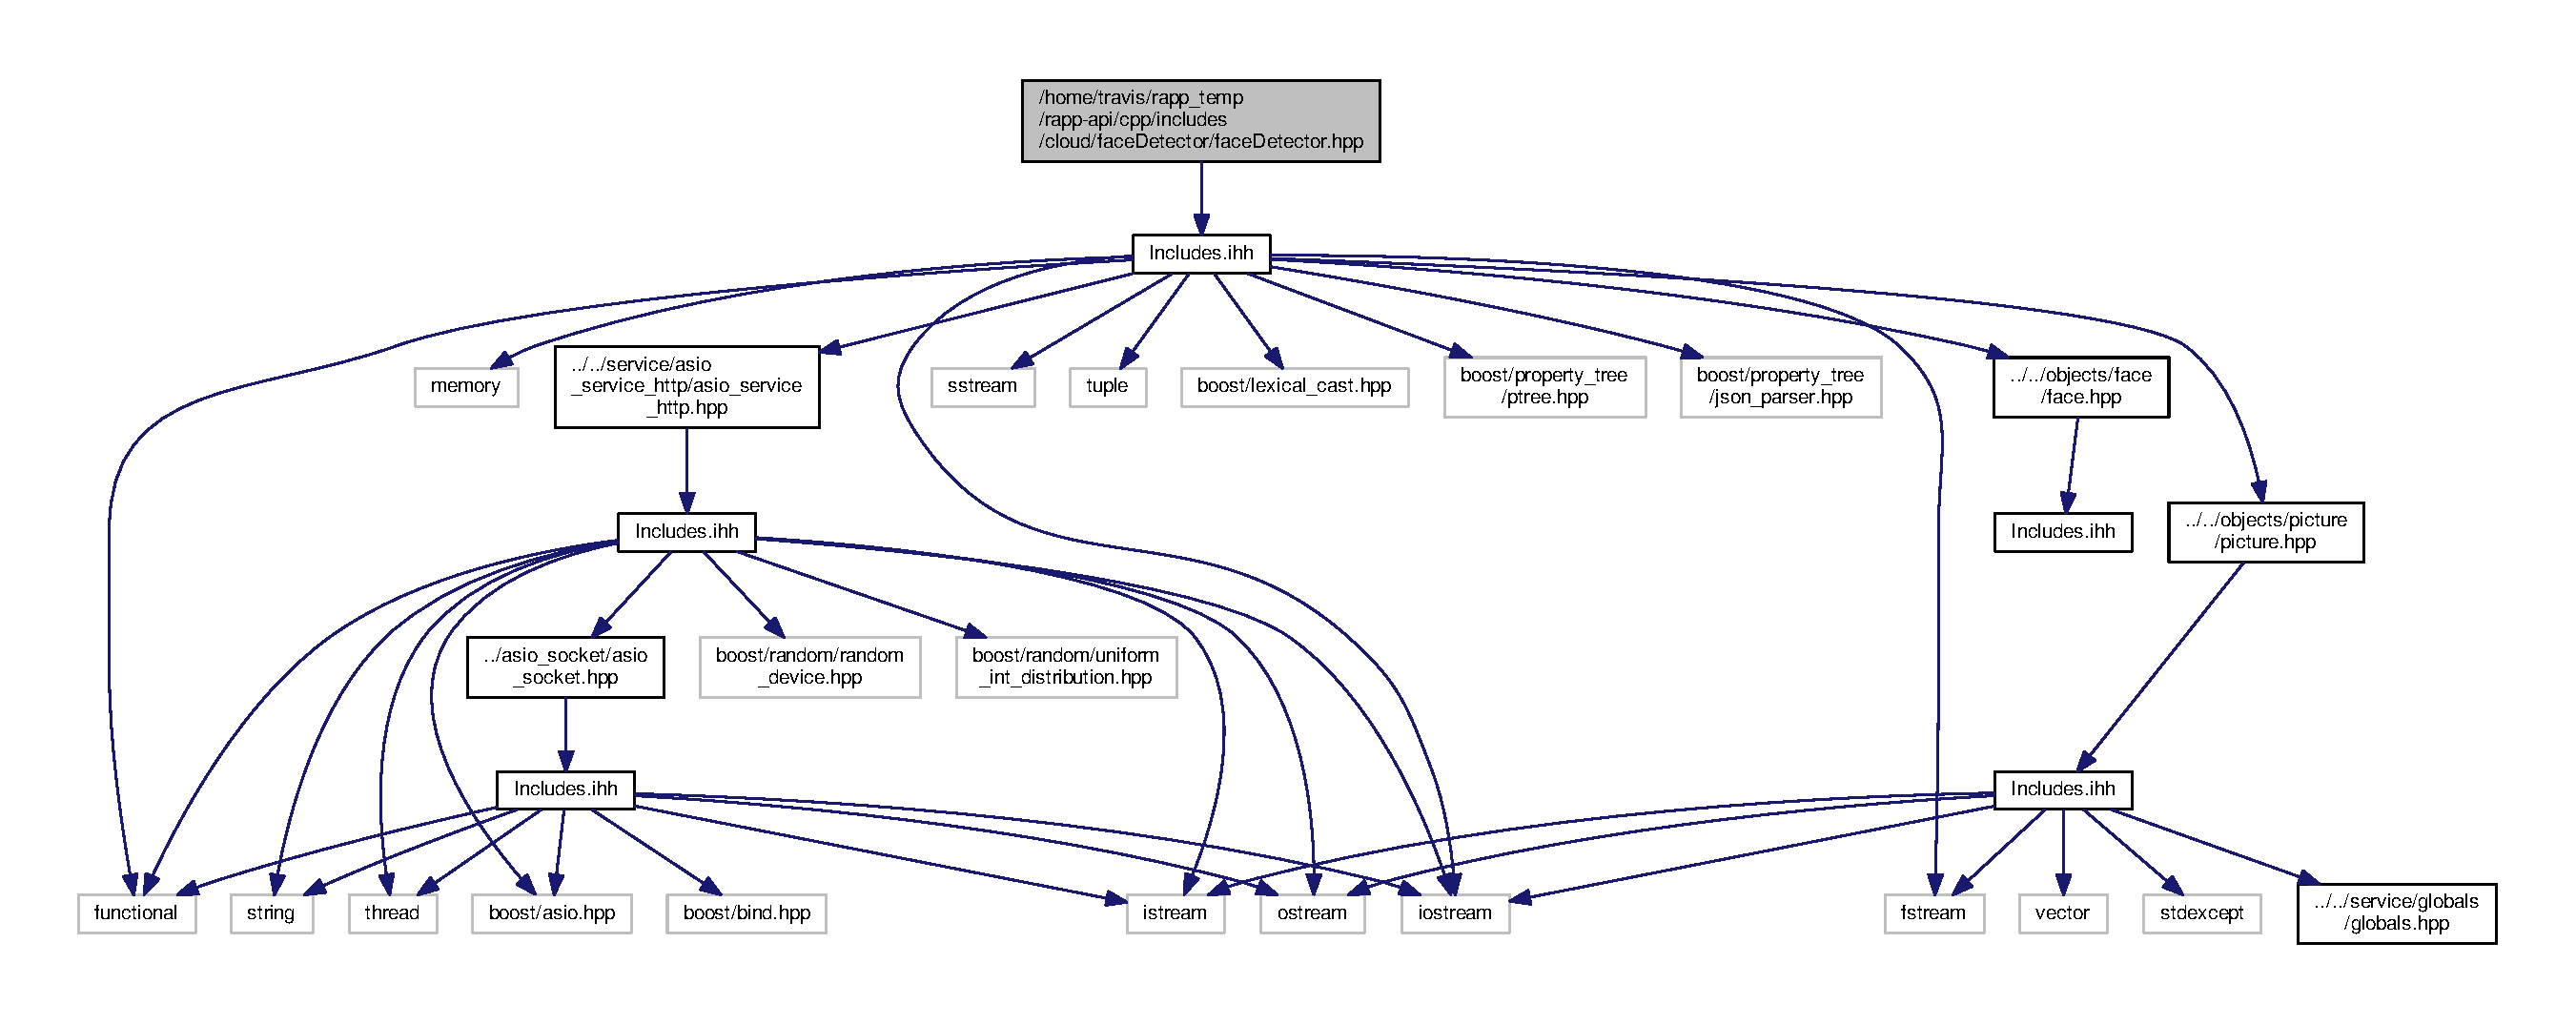
\includegraphics[width=350pt]{faceDetector_8hpp__incl}
\end{center}
\end{figure}
This graph shows which files directly or indirectly include this file\-:
\nopagebreak
\begin{figure}[H]
\begin{center}
\leavevmode
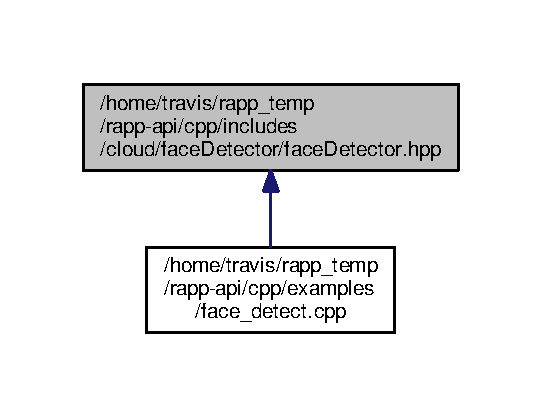
\includegraphics[width=260pt]{faceDetector_8hpp__dep__incl}
\end{center}
\end{figure}
\subsection*{Classes}
\begin{DoxyCompactItemize}
\item 
class \hyperlink{classrapp_1_1cloud_1_1faceDetector}{rapp\-::cloud\-::face\-Detector}
\begin{DoxyCompactList}\small\item\em Asynchronous Service which will request the cloud to detect faces. \end{DoxyCompactList}\end{DoxyCompactItemize}
\subsection*{Namespaces}
\begin{DoxyCompactItemize}
\item 
\hyperlink{namespacerapp}{rapp}
\item 
\hyperlink{namespacerapp_1_1cloud}{rapp\-::cloud}
\end{DoxyCompactItemize}

\hypertarget{cloud_2faceDetector_2Includes_8ihh}{\section{/home/travis/rapp\-\_\-temp/rapp-\/api/cpp/includes/cloud/face\-Detector/\-Includes.ihh File Reference}
\label{cloud_2faceDetector_2Includes_8ihh}\index{/home/travis/rapp\-\_\-temp/rapp-\/api/cpp/includes/cloud/face\-Detector/\-Includes.\-ihh@{/home/travis/rapp\-\_\-temp/rapp-\/api/cpp/includes/cloud/face\-Detector/\-Includes.\-ihh}}
}
{\ttfamily \#include $<$functional$>$}\\*
{\ttfamily \#include $<$memory$>$}\\*
{\ttfamily \#include $<$iostream$>$}\\*
{\ttfamily \#include $<$fstream$>$}\\*
{\ttfamily \#include $<$sstream$>$}\\*
{\ttfamily \#include $<$tuple$>$}\\*
{\ttfamily \#include $<$boost/lexical\-\_\-cast.\-hpp$>$}\\*
{\ttfamily \#include $<$boost/property\-\_\-tree/ptree.\-hpp$>$}\\*
{\ttfamily \#include $<$boost/property\-\_\-tree/json\-\_\-parser.\-hpp$>$}\\*
{\ttfamily \#include \char`\"{}../../service/asio\-\_\-service\-\_\-http/asio\-\_\-service\-\_\-http.\-hpp\char`\"{}}\\*
{\ttfamily \#include \char`\"{}../../objects/face/face.\-hpp\char`\"{}}\\*
{\ttfamily \#include \char`\"{}../../objects/picture/picture.\-hpp\char`\"{}}\\*
Include dependency graph for Includes.\-ihh\-:
\nopagebreak
\begin{figure}[H]
\begin{center}
\leavevmode
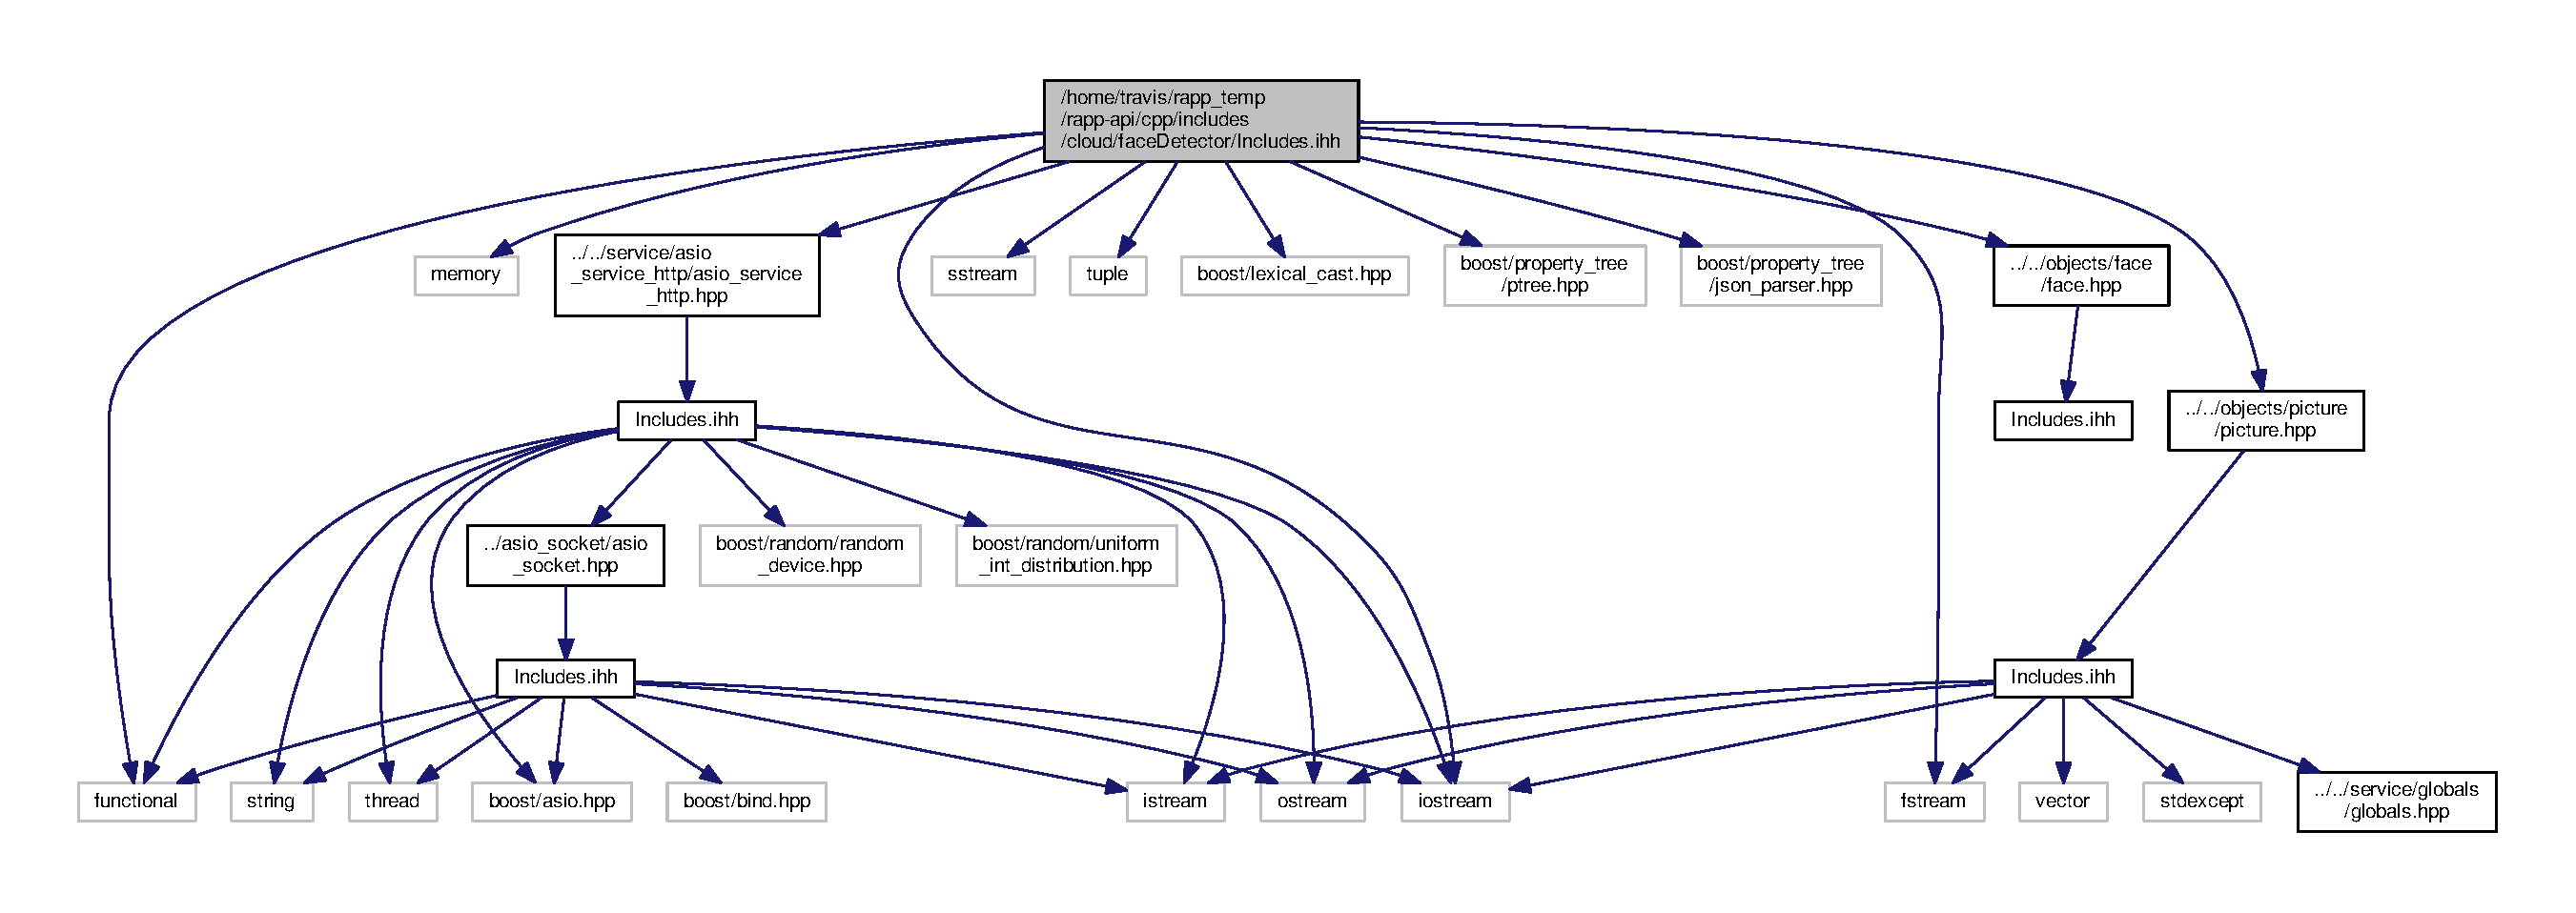
\includegraphics[width=350pt]{cloud_2faceDetector_2Includes_8ihh__incl}
\end{center}
\end{figure}
This graph shows which files directly or indirectly include this file\-:
\nopagebreak
\begin{figure}[H]
\begin{center}
\leavevmode
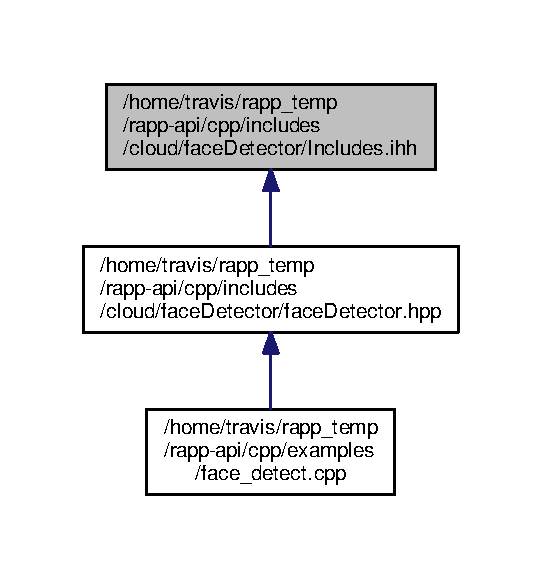
\includegraphics[width=260pt]{cloud_2faceDetector_2Includes_8ihh__dep__incl}
\end{center}
\end{figure}

\hypertarget{cloud_2fetchPersonalData_2Includes_8ihh}{\section{/home/travis/rapp\-\_\-temp/rapp-\/api/cpp/includes/cloud/fetch\-Personal\-Data/\-Includes.ihh File Reference}
\label{cloud_2fetchPersonalData_2Includes_8ihh}\index{/home/travis/rapp\-\_\-temp/rapp-\/api/cpp/includes/cloud/fetch\-Personal\-Data/\-Includes.\-ihh@{/home/travis/rapp\-\_\-temp/rapp-\/api/cpp/includes/cloud/fetch\-Personal\-Data/\-Includes.\-ihh}}
}
{\ttfamily \#include $<$functional$>$}\\*
{\ttfamily \#include $<$memory$>$}\\*
{\ttfamily \#include \char`\"{}../../service/asio\-\_\-service\-\_\-http/asio\-\_\-service\-\_\-http.\-hpp\char`\"{}}\\*
{\ttfamily \#include $<$boost/lexical\-\_\-cast.\-hpp$>$}\\*
Include dependency graph for Includes.\-ihh\-:
\nopagebreak
\begin{figure}[H]
\begin{center}
\leavevmode
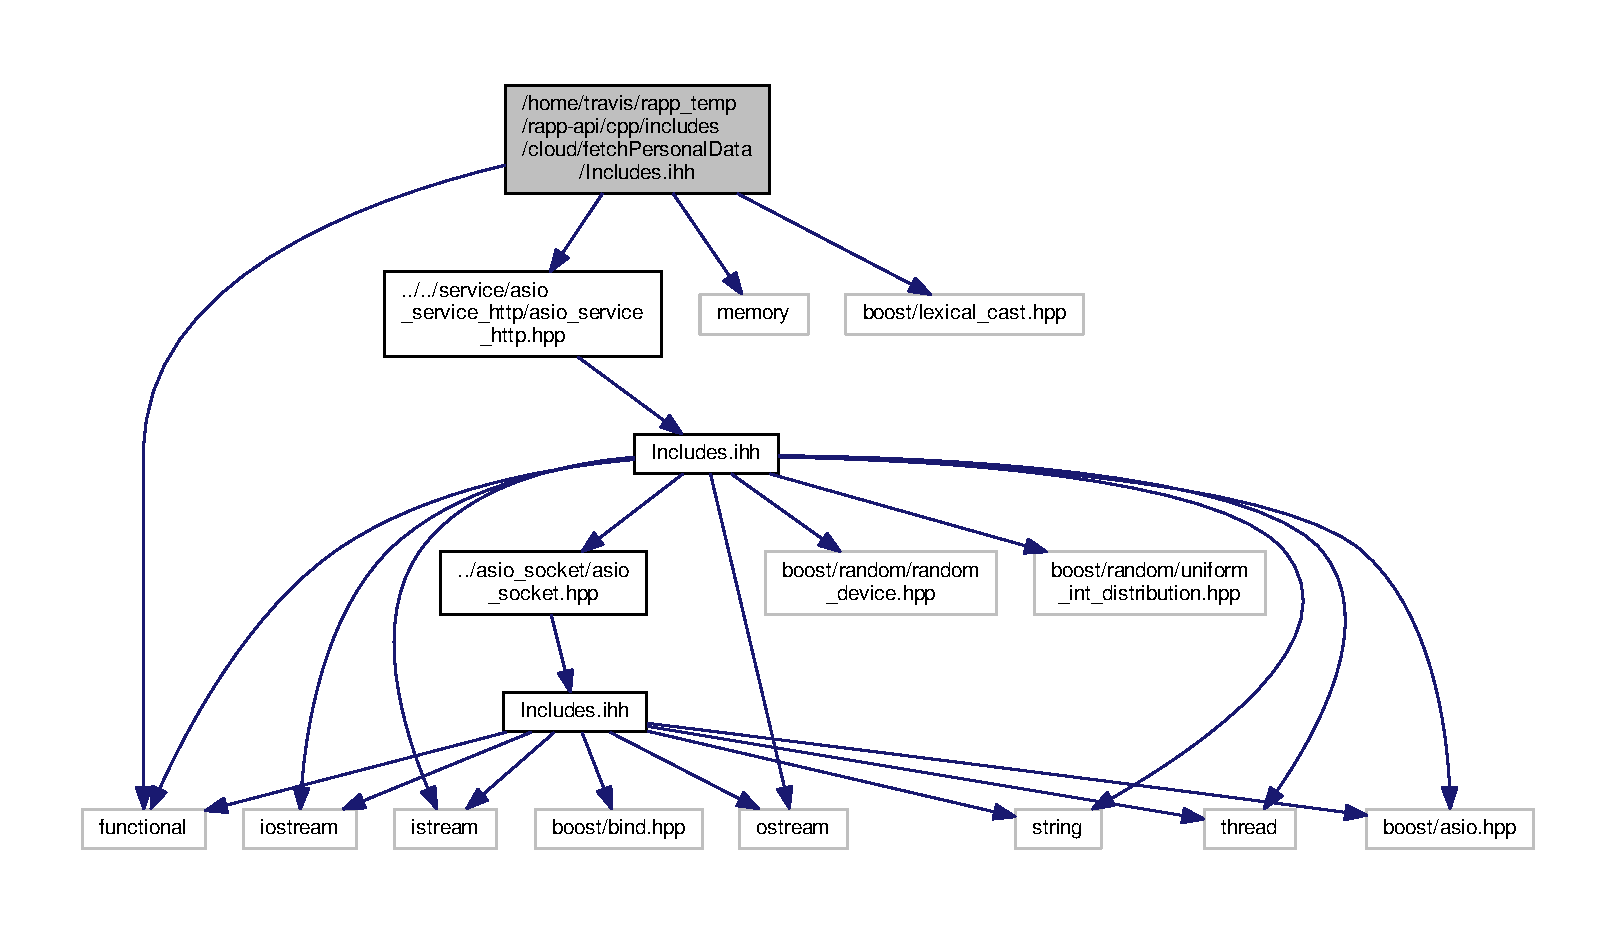
\includegraphics[width=350pt]{cloud_2fetchPersonalData_2Includes_8ihh__incl}
\end{center}
\end{figure}
This graph shows which files directly or indirectly include this file\-:
\nopagebreak
\begin{figure}[H]
\begin{center}
\leavevmode
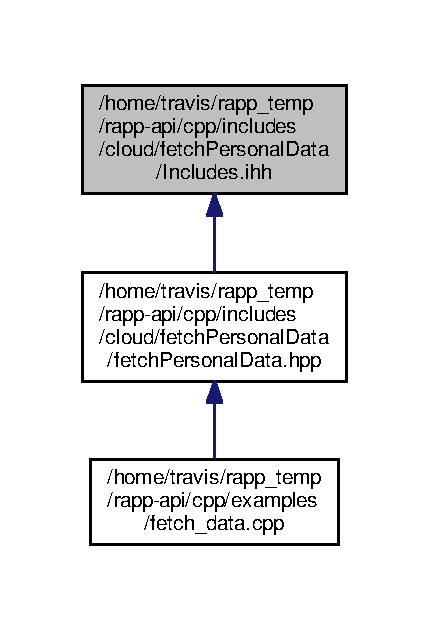
\includegraphics[width=206pt]{cloud_2fetchPersonalData_2Includes_8ihh__dep__incl}
\end{center}
\end{figure}

\hypertarget{cloud_2ontologyIsSubSuperClassOf_2Includes_8ihh}{\section{/home/travis/rapp\-\_\-temp/rapp-\/api/cpp/includes/cloud/ontology\-Is\-Sub\-Super\-Class\-Of/\-Includes.ihh File Reference}
\label{cloud_2ontologyIsSubSuperClassOf_2Includes_8ihh}\index{/home/travis/rapp\-\_\-temp/rapp-\/api/cpp/includes/cloud/ontology\-Is\-Sub\-Super\-Class\-Of/\-Includes.\-ihh@{/home/travis/rapp\-\_\-temp/rapp-\/api/cpp/includes/cloud/ontology\-Is\-Sub\-Super\-Class\-Of/\-Includes.\-ihh}}
}
This graph shows which files directly or indirectly include this file\-:
\nopagebreak
\begin{figure}[H]
\begin{center}
\leavevmode
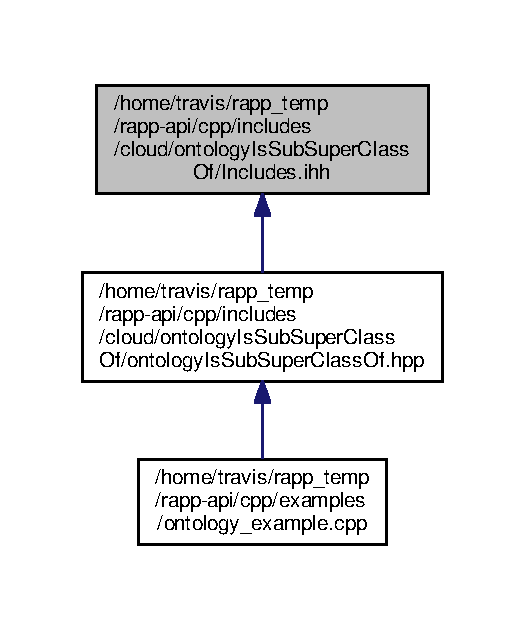
\includegraphics[width=252pt]{cloud_2ontologyIsSubSuperClassOf_2Includes_8ihh__dep__incl}
\end{center}
\end{figure}

\hypertarget{cloud_2ontologySubClassesOf_2Includes_8ihh}{\section{/home/travis/rapp\-\_\-temp/rapp-\/api/cpp/includes/cloud/ontology\-Sub\-Classes\-Of/\-Includes.ihh File Reference}
\label{cloud_2ontologySubClassesOf_2Includes_8ihh}\index{/home/travis/rapp\-\_\-temp/rapp-\/api/cpp/includes/cloud/ontology\-Sub\-Classes\-Of/\-Includes.\-ihh@{/home/travis/rapp\-\_\-temp/rapp-\/api/cpp/includes/cloud/ontology\-Sub\-Classes\-Of/\-Includes.\-ihh}}
}
{\ttfamily \#include $<$functional$>$}\\*
{\ttfamily \#include $<$memory$>$}\\*
{\ttfamily \#include $<$vector$>$}\\*
{\ttfamily \#include $<$string$>$}\\*
{\ttfamily \#include $<$boost/lexical\-\_\-cast.\-hpp$>$}\\*
{\ttfamily \#include $<$boost/property\-\_\-tree/ptree.\-hpp$>$}\\*
{\ttfamily \#include $<$boost/property\-\_\-tree/json\-\_\-parser.\-hpp$>$}\\*
{\ttfamily \#include \char`\"{}../../service/asio\-\_\-service\-\_\-http/asio\-\_\-service\-\_\-http.\-hpp\char`\"{}}\\*
Include dependency graph for Includes.\-ihh\-:
\nopagebreak
\begin{figure}[H]
\begin{center}
\leavevmode
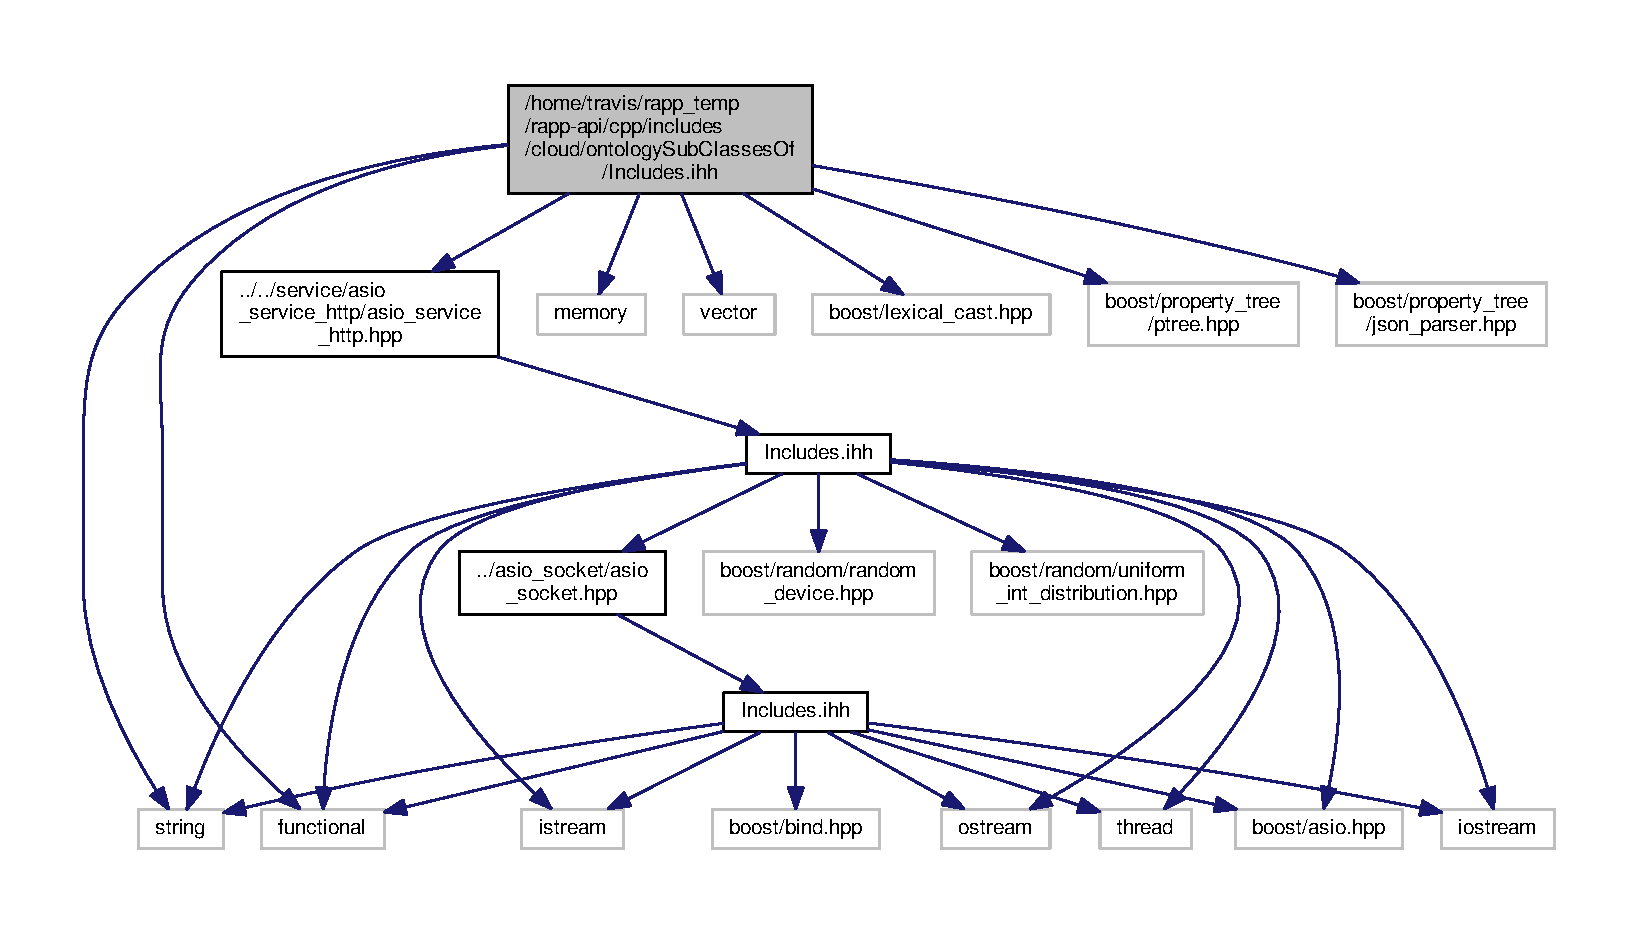
\includegraphics[width=350pt]{cloud_2ontologySubClassesOf_2Includes_8ihh__incl}
\end{center}
\end{figure}
This graph shows which files directly or indirectly include this file\-:
\nopagebreak
\begin{figure}[H]
\begin{center}
\leavevmode
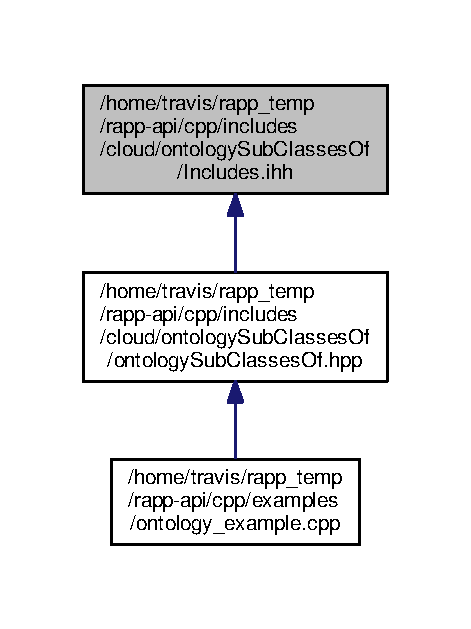
\includegraphics[width=226pt]{cloud_2ontologySubClassesOf_2Includes_8ihh__dep__incl}
\end{center}
\end{figure}

\hypertarget{cloud_2ontologySuperClassesOf_2Includes_8ihh}{\section{/home/travis/rapp\-\_\-temp/rapp-\/api/cpp/includes/cloud/ontology\-Super\-Classes\-Of/\-Includes.ihh File Reference}
\label{cloud_2ontologySuperClassesOf_2Includes_8ihh}\index{/home/travis/rapp\-\_\-temp/rapp-\/api/cpp/includes/cloud/ontology\-Super\-Classes\-Of/\-Includes.\-ihh@{/home/travis/rapp\-\_\-temp/rapp-\/api/cpp/includes/cloud/ontology\-Super\-Classes\-Of/\-Includes.\-ihh}}
}
{\ttfamily \#include $<$functional$>$}\\*
{\ttfamily \#include $<$memory$>$}\\*
{\ttfamily \#include $<$vector$>$}\\*
{\ttfamily \#include $<$string$>$}\\*
{\ttfamily \#include $<$boost/lexical\-\_\-cast.\-hpp$>$}\\*
{\ttfamily \#include $<$boost/property\-\_\-tree/ptree.\-hpp$>$}\\*
{\ttfamily \#include $<$boost/property\-\_\-tree/json\-\_\-parser.\-hpp$>$}\\*
{\ttfamily \#include \char`\"{}../../service/asio\-\_\-service\-\_\-http/asio\-\_\-service\-\_\-http.\-hpp\char`\"{}}\\*
Include dependency graph for Includes.\-ihh\-:
\nopagebreak
\begin{figure}[H]
\begin{center}
\leavevmode
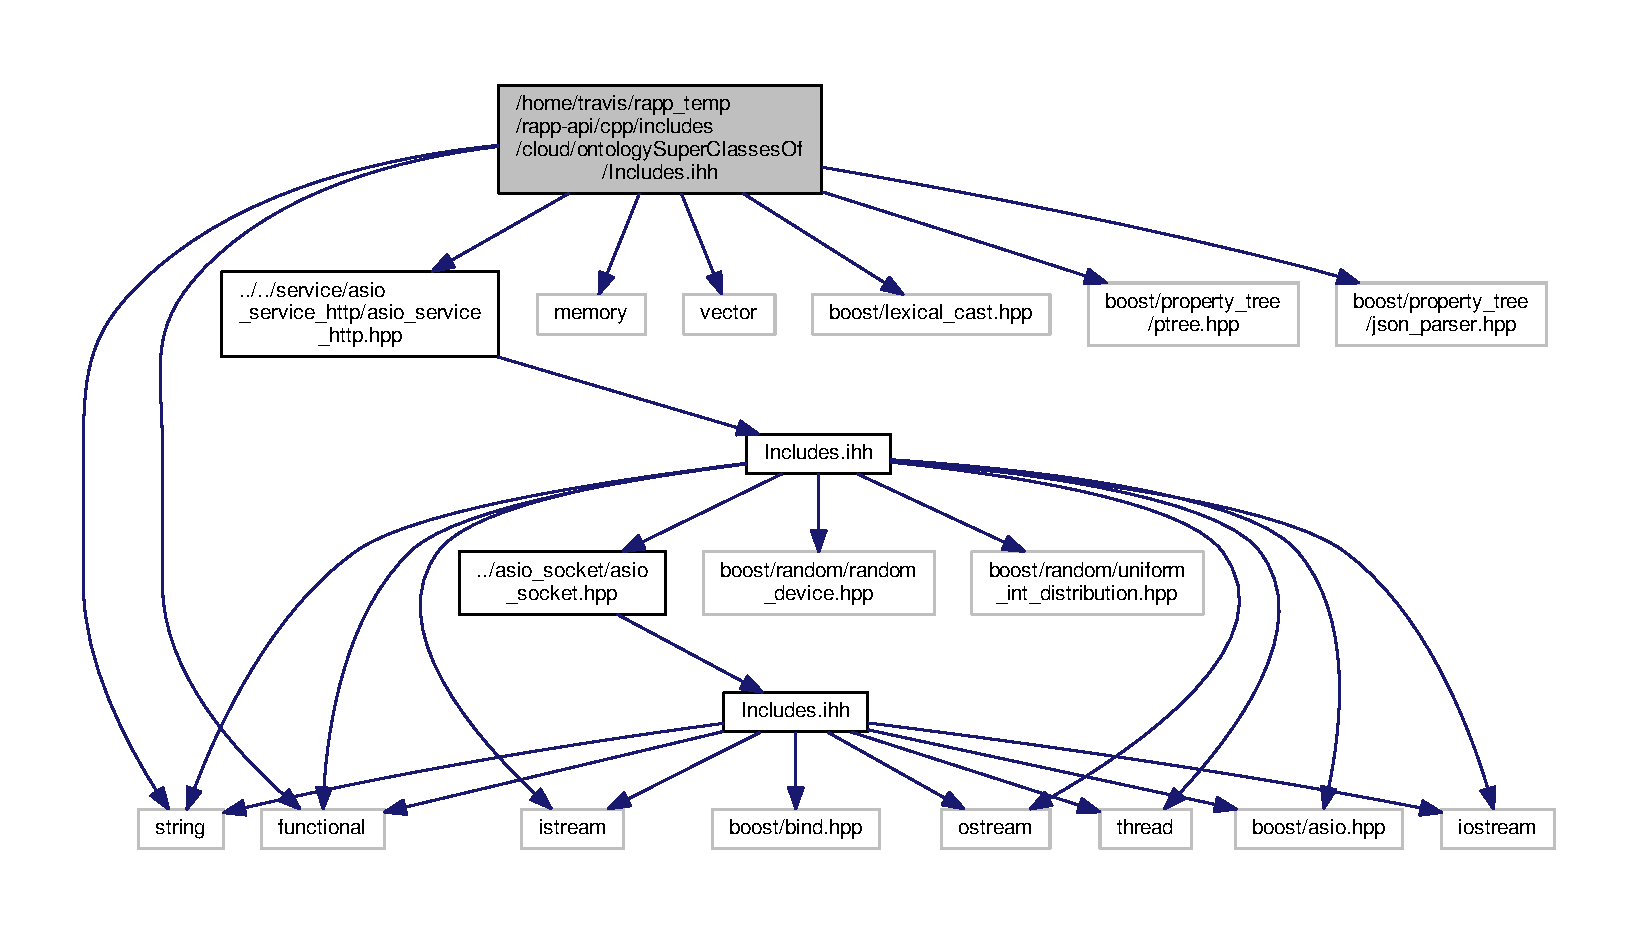
\includegraphics[width=350pt]{cloud_2ontologySuperClassesOf_2Includes_8ihh__incl}
\end{center}
\end{figure}
This graph shows which files directly or indirectly include this file\-:
\nopagebreak
\begin{figure}[H]
\begin{center}
\leavevmode
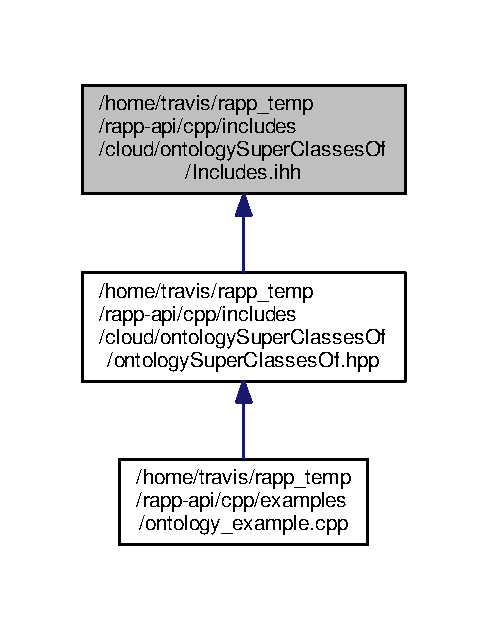
\includegraphics[width=234pt]{cloud_2ontologySuperClassesOf_2Includes_8ihh__dep__incl}
\end{center}
\end{figure}

\hypertarget{cloud_2qrDetector_2Includes_8ihh}{\section{/home/travis/rapp\-\_\-temp/rapp-\/api/cpp/includes/cloud/qr\-Detector/\-Includes.ihh File Reference}
\label{cloud_2qrDetector_2Includes_8ihh}\index{/home/travis/rapp\-\_\-temp/rapp-\/api/cpp/includes/cloud/qr\-Detector/\-Includes.\-ihh@{/home/travis/rapp\-\_\-temp/rapp-\/api/cpp/includes/cloud/qr\-Detector/\-Includes.\-ihh}}
}
{\ttfamily \#include $<$functional$>$}\\*
{\ttfamily \#include $<$memory$>$}\\*
{\ttfamily \#include $<$iostream$>$}\\*
{\ttfamily \#include $<$fstream$>$}\\*
{\ttfamily \#include $<$sstream$>$}\\*
{\ttfamily \#include $<$boost/lexical\-\_\-cast.\-hpp$>$}\\*
{\ttfamily \#include $<$boost/property\-\_\-tree/ptree.\-hpp$>$}\\*
{\ttfamily \#include $<$boost/property\-\_\-tree/json\-\_\-parser.\-hpp$>$}\\*
{\ttfamily \#include $<$boost/algorithm/string/replace.\-hpp$>$}\\*
{\ttfamily \#include \char`\"{}../../service/asio\-\_\-service\-\_\-http/asio\-\_\-service\-\_\-http.\-hpp\char`\"{}}\\*
{\ttfamily \#include \char`\"{}../../objects/qr\-Code/qr\-Code.\-hpp\char`\"{}}\\*
{\ttfamily \#include \char`\"{}../../objects/picture/picture.\-hpp\char`\"{}}\\*
Include dependency graph for Includes.\-ihh\-:
\nopagebreak
\begin{figure}[H]
\begin{center}
\leavevmode
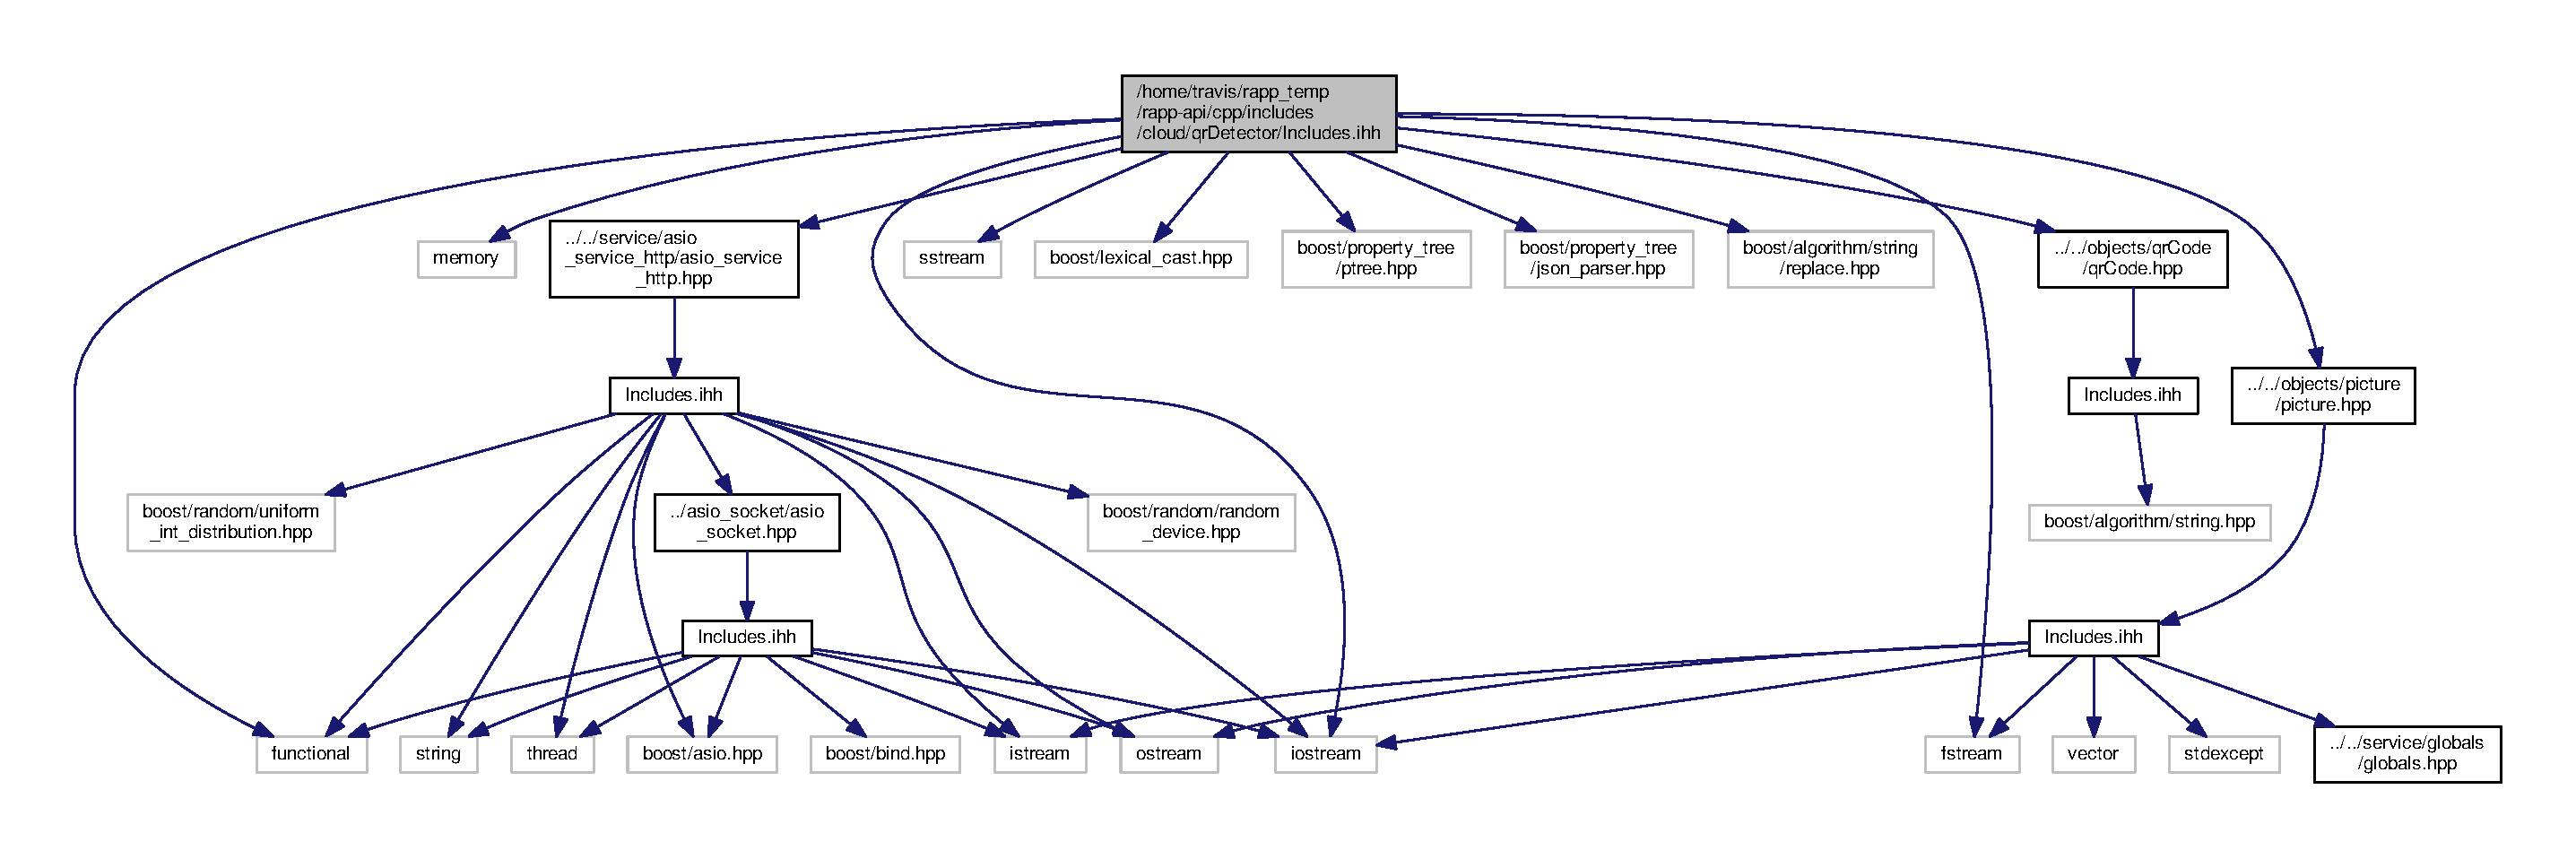
\includegraphics[width=350pt]{cloud_2qrDetector_2Includes_8ihh__incl}
\end{center}
\end{figure}
This graph shows which files directly or indirectly include this file\-:
\nopagebreak
\begin{figure}[H]
\begin{center}
\leavevmode
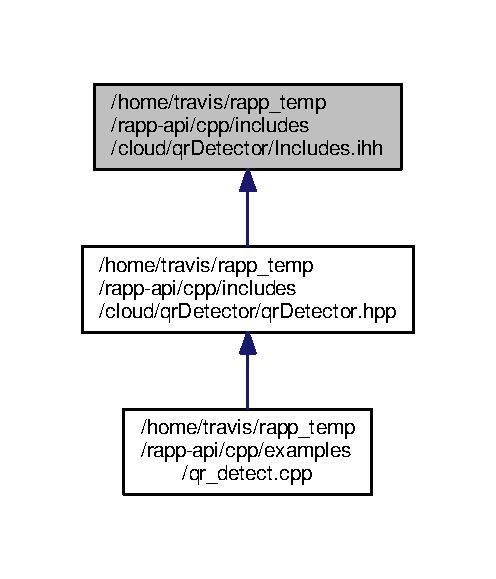
\includegraphics[width=238pt]{cloud_2qrDetector_2Includes_8ihh__dep__incl}
\end{center}
\end{figure}

\hypertarget{cloud_2setDenoiseProfile_2Includes_8ihh}{\section{/home/travis/rapp\-\_\-temp/rapp-\/api/cpp/includes/cloud/set\-Denoise\-Profile/\-Includes.ihh File Reference}
\label{cloud_2setDenoiseProfile_2Includes_8ihh}\index{/home/travis/rapp\-\_\-temp/rapp-\/api/cpp/includes/cloud/set\-Denoise\-Profile/\-Includes.\-ihh@{/home/travis/rapp\-\_\-temp/rapp-\/api/cpp/includes/cloud/set\-Denoise\-Profile/\-Includes.\-ihh}}
}
{\ttfamily \#include $<$functional$>$}\\*
{\ttfamily \#include $<$memory$>$}\\*
{\ttfamily \#include $<$iostream$>$}\\*
{\ttfamily \#include $<$fstream$>$}\\*
{\ttfamily \#include $<$sstream$>$}\\*
{\ttfamily \#include $<$boost/lexical\-\_\-cast.\-hpp$>$}\\*
{\ttfamily \#include $<$boost/property\-\_\-tree/ptree.\-hpp$>$}\\*
{\ttfamily \#include $<$boost/property\-\_\-tree/json\-\_\-parser.\-hpp$>$}\\*
{\ttfamily \#include \char`\"{}../../service/asio\-\_\-service\-\_\-http/asio\-\_\-service\-\_\-http.\-hpp\char`\"{}}\\*
{\ttfamily \#include \char`\"{}../../objects/audio/audio.\-hpp\char`\"{}}\\*
Include dependency graph for Includes.\-ihh\-:
\nopagebreak
\begin{figure}[H]
\begin{center}
\leavevmode
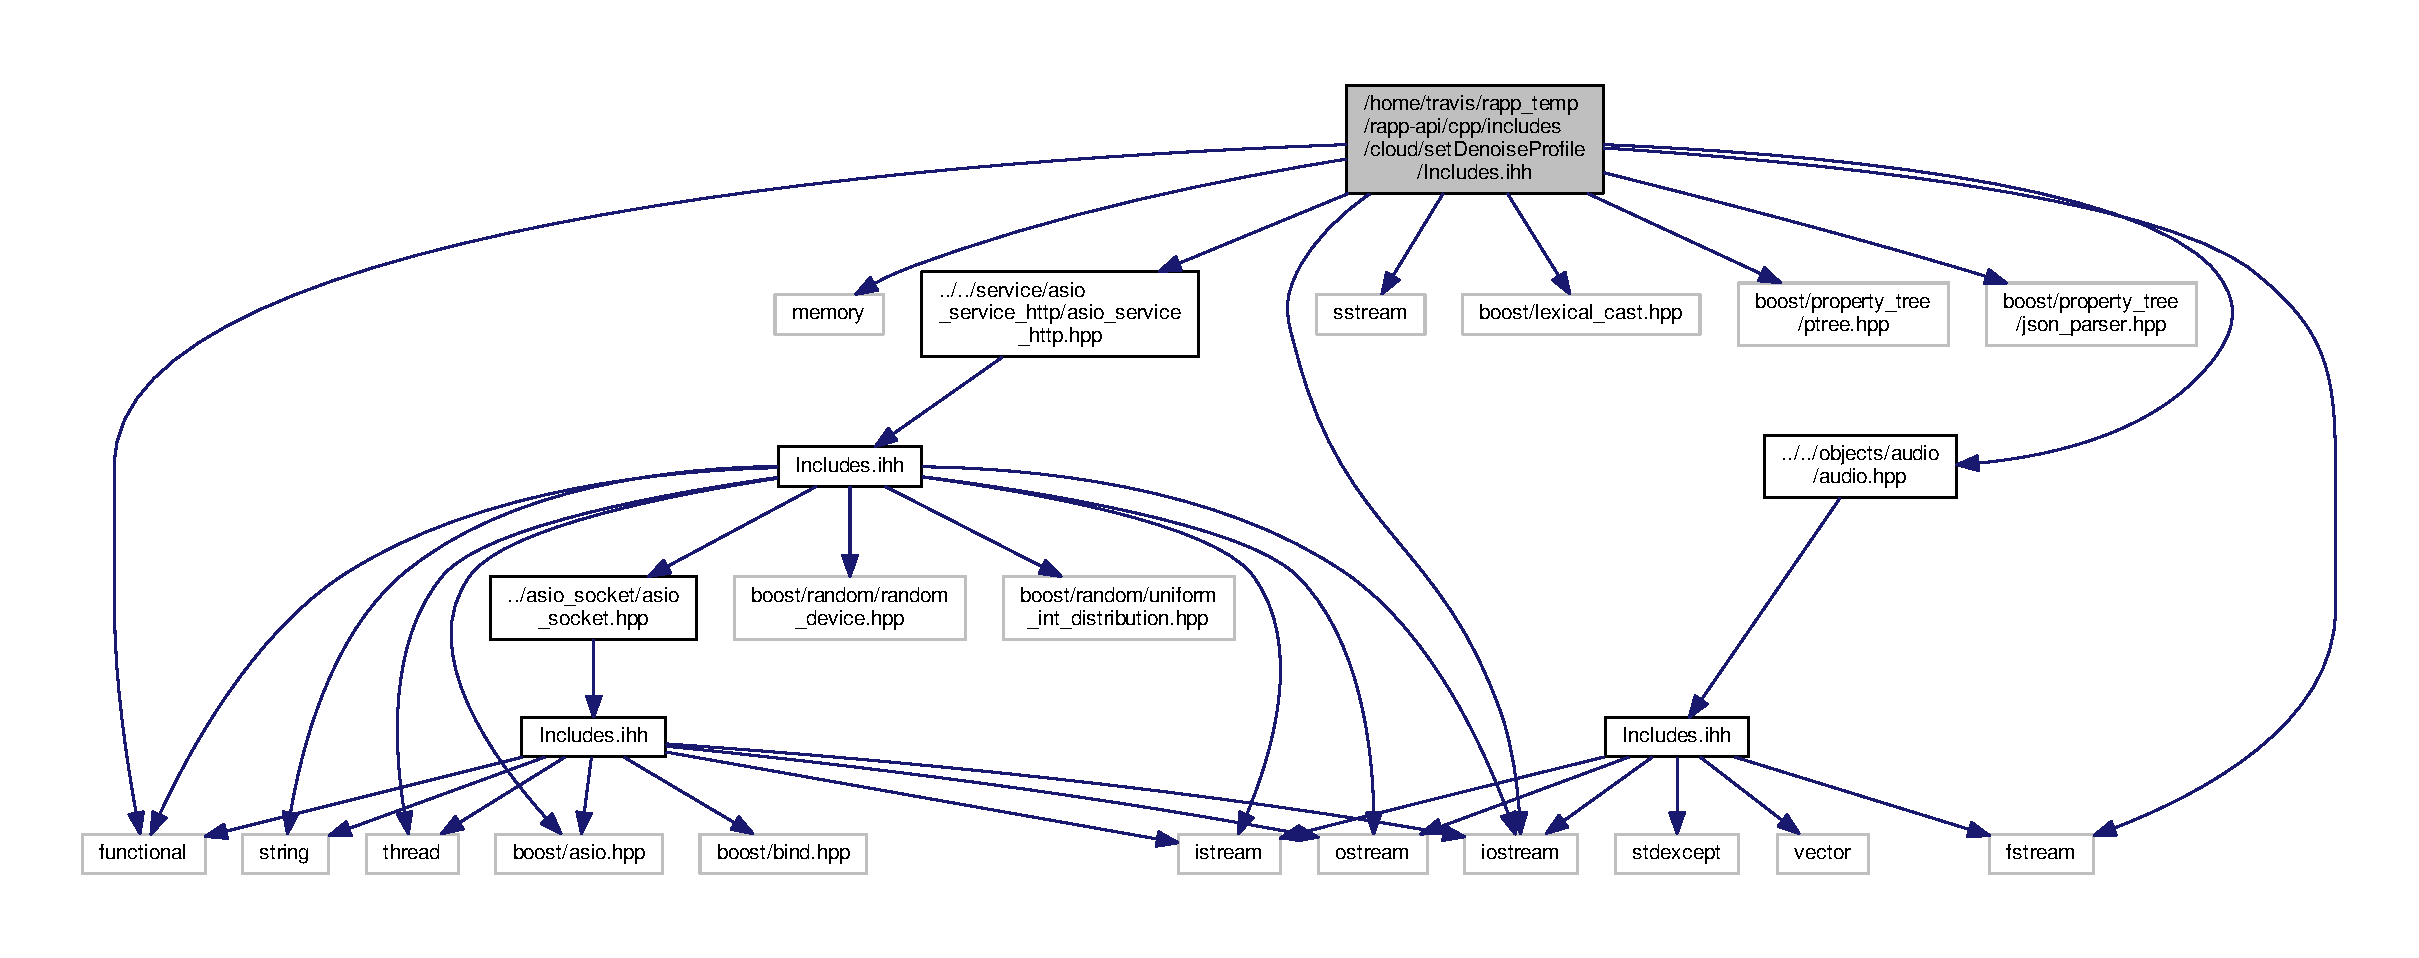
\includegraphics[width=350pt]{cloud_2setDenoiseProfile_2Includes_8ihh__incl}
\end{center}
\end{figure}
This graph shows which files directly or indirectly include this file\-:
\nopagebreak
\begin{figure}[H]
\begin{center}
\leavevmode
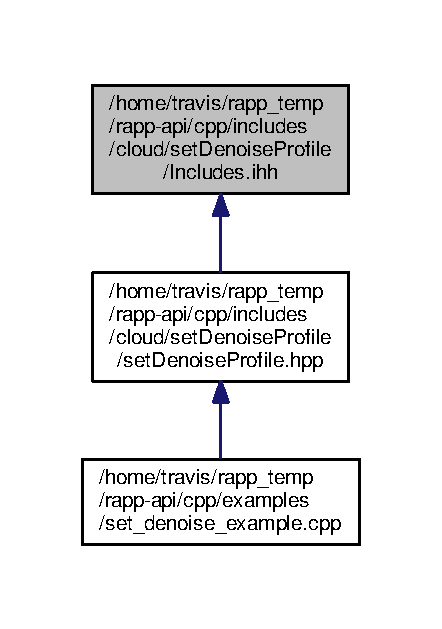
\includegraphics[width=212pt]{cloud_2setDenoiseProfile_2Includes_8ihh__dep__incl}
\end{center}
\end{figure}

\hypertarget{cloud_2speechToText_2Includes_8ihh}{\section{/home/travis/rapp\-\_\-temp/rapp-\/api/cpp/includes/cloud/speech\-To\-Text/\-Includes.ihh File Reference}
\label{cloud_2speechToText_2Includes_8ihh}\index{/home/travis/rapp\-\_\-temp/rapp-\/api/cpp/includes/cloud/speech\-To\-Text/\-Includes.\-ihh@{/home/travis/rapp\-\_\-temp/rapp-\/api/cpp/includes/cloud/speech\-To\-Text/\-Includes.\-ihh}}
}
{\ttfamily \#include $<$functional$>$}\\*
{\ttfamily \#include $<$memory$>$}\\*
{\ttfamily \#include $<$iostream$>$}\\*
{\ttfamily \#include $<$fstream$>$}\\*
{\ttfamily \#include $<$sstream$>$}\\*
{\ttfamily \#include $<$boost/lexical\-\_\-cast.\-hpp$>$}\\*
{\ttfamily \#include $<$boost/property\-\_\-tree/ptree.\-hpp$>$}\\*
{\ttfamily \#include $<$boost/property\-\_\-tree/json\-\_\-parser.\-hpp$>$}\\*
{\ttfamily \#include \char`\"{}../../service/asio\-\_\-service\-\_\-http/asio\-\_\-service\-\_\-http.\-hpp\char`\"{}}\\*
{\ttfamily \#include \char`\"{}../../objects/audio/audio.\-hpp\char`\"{}}\\*
Include dependency graph for Includes.\-ihh\-:
\nopagebreak
\begin{figure}[H]
\begin{center}
\leavevmode
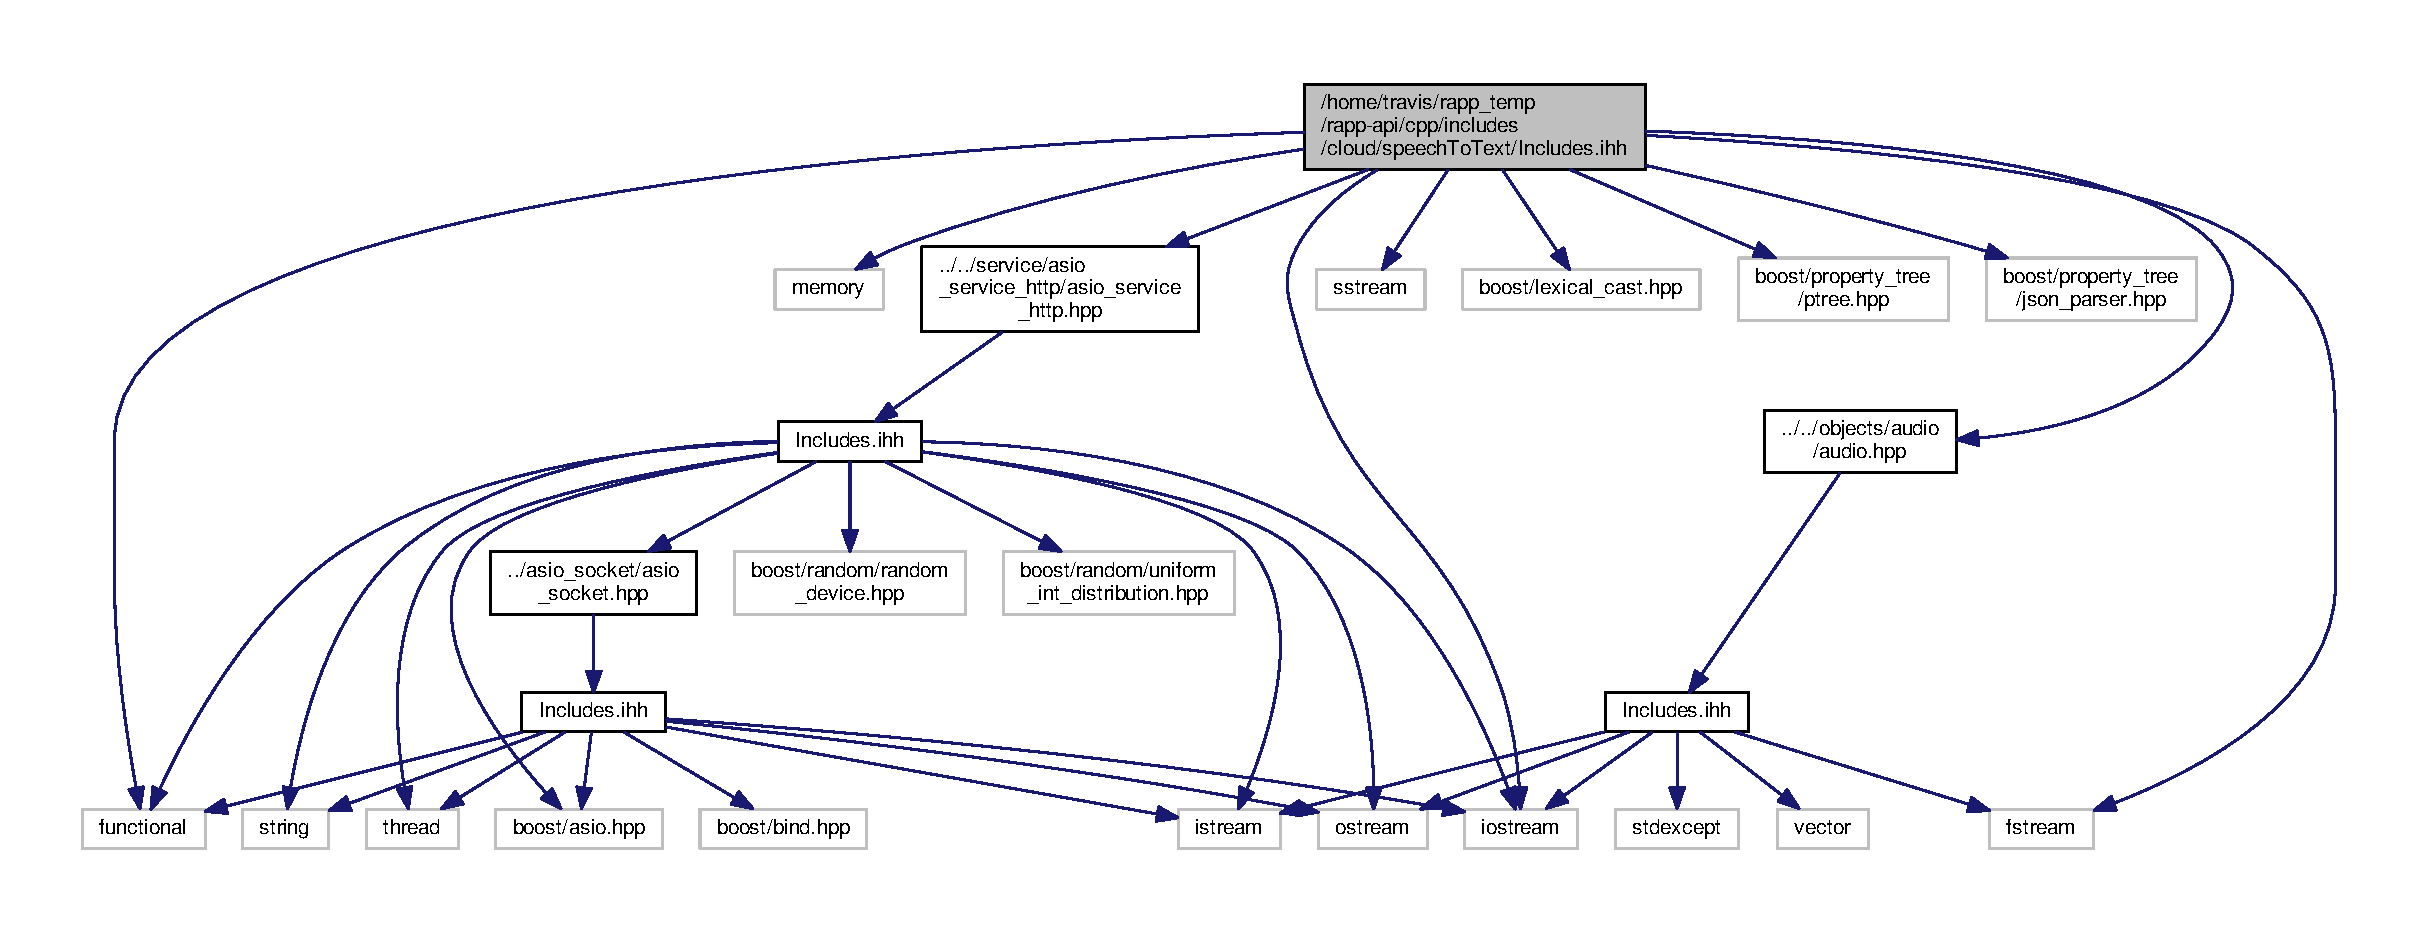
\includegraphics[width=350pt]{cloud_2speechToText_2Includes_8ihh__incl}
\end{center}
\end{figure}
This graph shows which files directly or indirectly include this file\-:
\nopagebreak
\begin{figure}[H]
\begin{center}
\leavevmode
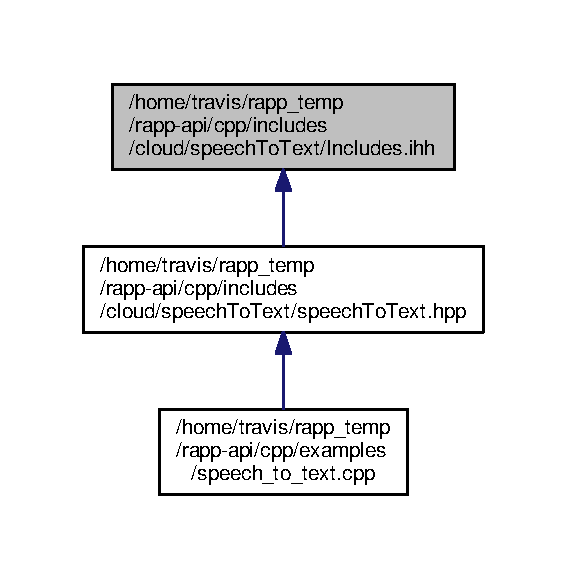
\includegraphics[width=272pt]{cloud_2speechToText_2Includes_8ihh__dep__incl}
\end{center}
\end{figure}

\hypertarget{cloud_2upServices_2Includes_8ihh}{\section{/home/travis/rapp\-\_\-temp/rapp-\/api/cpp/includes/cloud/up\-Services/\-Includes.ihh File Reference}
\label{cloud_2upServices_2Includes_8ihh}\index{/home/travis/rapp\-\_\-temp/rapp-\/api/cpp/includes/cloud/up\-Services/\-Includes.\-ihh@{/home/travis/rapp\-\_\-temp/rapp-\/api/cpp/includes/cloud/up\-Services/\-Includes.\-ihh}}
}

\hypertarget{objects_2audio_2Includes_8ihh}{\section{/home/travis/rapp\-\_\-temp/rapp-\/api/cpp/includes/objects/audio/\-Includes.ihh File Reference}
\label{objects_2audio_2Includes_8ihh}\index{/home/travis/rapp\-\_\-temp/rapp-\/api/cpp/includes/objects/audio/\-Includes.\-ihh@{/home/travis/rapp\-\_\-temp/rapp-\/api/cpp/includes/objects/audio/\-Includes.\-ihh}}
}
{\ttfamily \#include $<$iostream$>$}\\*
{\ttfamily \#include $<$istream$>$}\\*
{\ttfamily \#include $<$ostream$>$}\\*
{\ttfamily \#include $<$fstream$>$}\\*
{\ttfamily \#include $<$vector$>$}\\*
{\ttfamily \#include $<$stdexcept$>$}\\*
Include dependency graph for Includes.\-ihh\-:
\nopagebreak
\begin{figure}[H]
\begin{center}
\leavevmode
\includegraphics[width=350pt]{objects_2audio_2Includes_8ihh__incl}
\end{center}
\end{figure}
This graph shows which files directly or indirectly include this file\-:
\nopagebreak
\begin{figure}[H]
\begin{center}
\leavevmode
\includegraphics[width=350pt]{objects_2audio_2Includes_8ihh__dep__incl}
\end{center}
\end{figure}

\hypertarget{objects_2face_2Includes_8ihh}{\section{/home/travis/rapp\-\_\-temp/rapp-\/api/cpp/includes/objects/face/\-Includes.ihh File Reference}
\label{objects_2face_2Includes_8ihh}\index{/home/travis/rapp\-\_\-temp/rapp-\/api/cpp/includes/objects/face/\-Includes.\-ihh@{/home/travis/rapp\-\_\-temp/rapp-\/api/cpp/includes/objects/face/\-Includes.\-ihh}}
}
This graph shows which files directly or indirectly include this file\-:
\nopagebreak
\begin{figure}[H]
\begin{center}
\leavevmode
\includegraphics[width=260pt]{objects_2face_2Includes_8ihh__dep__incl}
\end{center}
\end{figure}

\hypertarget{objects_2picture_2Includes_8ihh}{\section{/home/travis/rapp\-\_\-temp/rapp-\/api/cpp/includes/objects/picture/\-Includes.ihh File Reference}
\label{objects_2picture_2Includes_8ihh}\index{/home/travis/rapp\-\_\-temp/rapp-\/api/cpp/includes/objects/picture/\-Includes.\-ihh@{/home/travis/rapp\-\_\-temp/rapp-\/api/cpp/includes/objects/picture/\-Includes.\-ihh}}
}
{\ttfamily \#include $<$iostream$>$}\\*
{\ttfamily \#include $<$istream$>$}\\*
{\ttfamily \#include $<$ostream$>$}\\*
{\ttfamily \#include $<$fstream$>$}\\*
{\ttfamily \#include $<$vector$>$}\\*
{\ttfamily \#include $<$stdexcept$>$}\\*
{\ttfamily \#include \char`\"{}../../service/globals/globals.\-hpp\char`\"{}}\\*
Include dependency graph for Includes.\-ihh\-:
\nopagebreak
\begin{figure}[H]
\begin{center}
\leavevmode
\includegraphics[width=350pt]{objects_2picture_2Includes_8ihh__incl}
\end{center}
\end{figure}
This graph shows which files directly or indirectly include this file\-:
\nopagebreak
\begin{figure}[H]
\begin{center}
\leavevmode
\includegraphics[width=350pt]{objects_2picture_2Includes_8ihh__dep__incl}
\end{center}
\end{figure}

\hypertarget{objects_2qrCode_2Includes_8ihh}{\section{/home/travis/rapp\-\_\-temp/rapp-\/api/cpp/includes/objects/qr\-Code/\-Includes.ihh File Reference}
\label{objects_2qrCode_2Includes_8ihh}\index{/home/travis/rapp\-\_\-temp/rapp-\/api/cpp/includes/objects/qr\-Code/\-Includes.\-ihh@{/home/travis/rapp\-\_\-temp/rapp-\/api/cpp/includes/objects/qr\-Code/\-Includes.\-ihh}}
}
{\ttfamily \#include $<$boost/algorithm/string.\-hpp$>$}\\*
Include dependency graph for Includes.\-ihh\-:
\nopagebreak
\begin{figure}[H]
\begin{center}
\leavevmode
\includegraphics[width=220pt]{objects_2qrCode_2Includes_8ihh__incl}
\end{center}
\end{figure}
This graph shows which files directly or indirectly include this file\-:
\nopagebreak
\begin{figure}[H]
\begin{center}
\leavevmode
\includegraphics[width=238pt]{objects_2qrCode_2Includes_8ihh__dep__incl}
\end{center}
\end{figure}

\hypertarget{robot_2communication_2Includes_8ihh}{\section{/home/travis/rapp\-\_\-temp/rapp-\/api/cpp/includes/robot/communication/\-Includes.ihh File Reference}
\label{robot_2communication_2Includes_8ihh}\index{/home/travis/rapp\-\_\-temp/rapp-\/api/cpp/includes/robot/communication/\-Includes.\-ihh@{/home/travis/rapp\-\_\-temp/rapp-\/api/cpp/includes/robot/communication/\-Includes.\-ihh}}
}
{\ttfamily \#include \char`\"{}../../objects/audio/audio.\-hpp\char`\"{}}\\*
Include dependency graph for Includes.\-ihh\-:
\nopagebreak
\begin{figure}[H]
\begin{center}
\leavevmode
\includegraphics[width=350pt]{robot_2communication_2Includes_8ihh__incl}
\end{center}
\end{figure}
This graph shows which files directly or indirectly include this file\-:
\nopagebreak
\begin{figure}[H]
\begin{center}
\leavevmode
\includegraphics[width=278pt]{robot_2communication_2Includes_8ihh__dep__incl}
\end{center}
\end{figure}

\hypertarget{robot_2nao_2Includes_8ihh}{\section{/home/travis/rapp\-\_\-temp/rapp-\/api/cpp/includes/robot/nao/\-Includes.ihh File Reference}
\label{robot_2nao_2Includes_8ihh}\index{/home/travis/rapp\-\_\-temp/rapp-\/api/cpp/includes/robot/nao/\-Includes.\-ihh@{/home/travis/rapp\-\_\-temp/rapp-\/api/cpp/includes/robot/nao/\-Includes.\-ihh}}
}
This graph shows which files directly or indirectly include this file\-:
\nopagebreak
\begin{figure}[H]
\begin{center}
\leavevmode
\includegraphics[width=198pt]{robot_2nao_2Includes_8ihh__dep__incl}
\end{center}
\end{figure}

\hypertarget{robot_2navigation_2Includes_8ihh}{\section{/home/travis/rapp\-\_\-temp/rapp-\/api/cpp/includes/robot/navigation/\-Includes.ihh File Reference}
\label{robot_2navigation_2Includes_8ihh}\index{/home/travis/rapp\-\_\-temp/rapp-\/api/cpp/includes/robot/navigation/\-Includes.\-ihh@{/home/travis/rapp\-\_\-temp/rapp-\/api/cpp/includes/robot/navigation/\-Includes.\-ihh}}
}
This graph shows which files directly or indirectly include this file\-:
\nopagebreak
\begin{figure}[H]
\begin{center}
\leavevmode
\includegraphics[width=234pt]{robot_2navigation_2Includes_8ihh__dep__incl}
\end{center}
\end{figure}

\hypertarget{robot_2proto_2Includes_8ihh}{\section{/home/travis/rapp\-\_\-temp/rapp-\/api/cpp/includes/robot/proto/\-Includes.ihh File Reference}
\label{robot_2proto_2Includes_8ihh}\index{/home/travis/rapp\-\_\-temp/rapp-\/api/cpp/includes/robot/proto/\-Includes.\-ihh@{/home/travis/rapp\-\_\-temp/rapp-\/api/cpp/includes/robot/proto/\-Includes.\-ihh}}
}
This graph shows which files directly or indirectly include this file\-:
\nopagebreak
\begin{figure}[H]
\begin{center}
\leavevmode
\includegraphics[width=202pt]{robot_2proto_2Includes_8ihh__dep__incl}
\end{center}
\end{figure}

\hypertarget{robot_2vision_2Includes_8ihh}{\section{/home/travis/rapp\-\_\-temp/rapp-\/api/cpp/includes/robot/vision/\-Includes.ihh File Reference}
\label{robot_2vision_2Includes_8ihh}\index{/home/travis/rapp\-\_\-temp/rapp-\/api/cpp/includes/robot/vision/\-Includes.\-ihh@{/home/travis/rapp\-\_\-temp/rapp-\/api/cpp/includes/robot/vision/\-Includes.\-ihh}}
}
{\ttfamily \#include \char`\"{}../../objects/picture/picture.\-hpp\char`\"{}}\\*
Include dependency graph for Includes.\-ihh\-:
\nopagebreak
\begin{figure}[H]
\begin{center}
\leavevmode
\includegraphics[width=350pt]{robot_2vision_2Includes_8ihh__incl}
\end{center}
\end{figure}
This graph shows which files directly or indirectly include this file\-:
\nopagebreak
\begin{figure}[H]
\begin{center}
\leavevmode
\includegraphics[width=204pt]{robot_2vision_2Includes_8ihh__dep__incl}
\end{center}
\end{figure}

\hypertarget{service_2asio__service__http_2Includes_8ihh}{\section{/home/travis/rapp\-\_\-temp/rapp-\/api/cpp/includes/service/asio\-\_\-service\-\_\-http/\-Includes.ihh File Reference}
\label{service_2asio__service__http_2Includes_8ihh}\index{/home/travis/rapp\-\_\-temp/rapp-\/api/cpp/includes/service/asio\-\_\-service\-\_\-http/\-Includes.\-ihh@{/home/travis/rapp\-\_\-temp/rapp-\/api/cpp/includes/service/asio\-\_\-service\-\_\-http/\-Includes.\-ihh}}
}
{\ttfamily \#include $<$iostream$>$}\\*
{\ttfamily \#include $<$istream$>$}\\*
{\ttfamily \#include $<$ostream$>$}\\*
{\ttfamily \#include $<$string$>$}\\*
{\ttfamily \#include $<$functional$>$}\\*
{\ttfamily \#include $<$thread$>$}\\*
{\ttfamily \#include $<$boost/asio.\-hpp$>$}\\*
{\ttfamily \#include $<$boost/random/random\-\_\-device.\-hpp$>$}\\*
{\ttfamily \#include $<$boost/random/uniform\-\_\-int\-\_\-distribution.\-hpp$>$}\\*
{\ttfamily \#include \char`\"{}../asio\-\_\-socket/asio\-\_\-socket.\-hpp\char`\"{}}\\*
Include dependency graph for Includes.\-ihh\-:
\nopagebreak
\begin{figure}[H]
\begin{center}
\leavevmode
\includegraphics[width=350pt]{service_2asio__service__http_2Includes_8ihh__incl}
\end{center}
\end{figure}
This graph shows which files directly or indirectly include this file\-:
\nopagebreak
\begin{figure}[H]
\begin{center}
\leavevmode
\includegraphics[width=350pt]{service_2asio__service__http_2Includes_8ihh__dep__incl}
\end{center}
\end{figure}

\hypertarget{service_2asio__service__raw_2Includes_8ihh}{\section{/home/travis/rapp\-\_\-temp/rapp-\/api/cpp/includes/service/asio\-\_\-service\-\_\-raw/\-Includes.ihh File Reference}
\label{service_2asio__service__raw_2Includes_8ihh}\index{/home/travis/rapp\-\_\-temp/rapp-\/api/cpp/includes/service/asio\-\_\-service\-\_\-raw/\-Includes.\-ihh@{/home/travis/rapp\-\_\-temp/rapp-\/api/cpp/includes/service/asio\-\_\-service\-\_\-raw/\-Includes.\-ihh}}
}
{\ttfamily \#include $<$iostream$>$}\\*
{\ttfamily \#include $<$istream$>$}\\*
{\ttfamily \#include $<$ostream$>$}\\*
{\ttfamily \#include $<$fstream$>$}\\*
{\ttfamily \#include $<$string$>$}\\*
{\ttfamily \#include $<$functional$>$}\\*
{\ttfamily \#include $<$thread$>$}\\*
{\ttfamily \#include $<$boost/asio.\-hpp$>$}\\*
{\ttfamily \#include $<$boost/bind.\-hpp$>$}\\*
{\ttfamily \#include \char`\"{}../asio\-\_\-socket/asio\-\_\-socket.\-hpp\char`\"{}}\\*
{\ttfamily \#include \char`\"{}../globals/globals.\-hpp\char`\"{}}\\*
Include dependency graph for Includes.\-ihh\-:
\nopagebreak
\begin{figure}[H]
\begin{center}
\leavevmode
\includegraphics[width=350pt]{service_2asio__service__raw_2Includes_8ihh__incl}
\end{center}
\end{figure}
This graph shows which files directly or indirectly include this file\-:
\nopagebreak
\begin{figure}[H]
\begin{center}
\leavevmode
\includegraphics[width=210pt]{service_2asio__service__raw_2Includes_8ihh__dep__incl}
\end{center}
\end{figure}

\hypertarget{service_2asio__socket_2Includes_8ihh}{\section{/home/travis/rapp\-\_\-temp/rapp-\/api/cpp/includes/service/asio\-\_\-socket/\-Includes.ihh File Reference}
\label{service_2asio__socket_2Includes_8ihh}\index{/home/travis/rapp\-\_\-temp/rapp-\/api/cpp/includes/service/asio\-\_\-socket/\-Includes.\-ihh@{/home/travis/rapp\-\_\-temp/rapp-\/api/cpp/includes/service/asio\-\_\-socket/\-Includes.\-ihh}}
}
{\ttfamily \#include $<$iostream$>$}\\*
{\ttfamily \#include $<$istream$>$}\\*
{\ttfamily \#include $<$ostream$>$}\\*
{\ttfamily \#include $<$string$>$}\\*
{\ttfamily \#include $<$functional$>$}\\*
{\ttfamily \#include $<$thread$>$}\\*
{\ttfamily \#include $<$boost/asio.\-hpp$>$}\\*
{\ttfamily \#include $<$boost/bind.\-hpp$>$}\\*
Include dependency graph for Includes.\-ihh\-:
\nopagebreak
\begin{figure}[H]
\begin{center}
\leavevmode
\includegraphics[width=350pt]{service_2asio__socket_2Includes_8ihh__incl}
\end{center}
\end{figure}
This graph shows which files directly or indirectly include this file\-:
\nopagebreak
\begin{figure}[H]
\begin{center}
\leavevmode
\includegraphics[width=350pt]{service_2asio__socket_2Includes_8ihh__dep__incl}
\end{center}
\end{figure}

\hypertarget{service_2service__controller_2Includes_8ihh}{\section{/home/travis/rapp\-\_\-temp/rapp-\/api/cpp/includes/service/service\-\_\-controller/\-Includes.ihh File Reference}
\label{service_2service__controller_2Includes_8ihh}\index{/home/travis/rapp\-\_\-temp/rapp-\/api/cpp/includes/service/service\-\_\-controller/\-Includes.\-ihh@{/home/travis/rapp\-\_\-temp/rapp-\/api/cpp/includes/service/service\-\_\-controller/\-Includes.\-ihh}}
}
{\ttfamily \#include $<$thread$>$}\\*
{\ttfamily \#include $<$functional$>$}\\*
{\ttfamily \#include $<$vector$>$}\\*
{\ttfamily \#include $<$memory$>$}\\*
{\ttfamily \#include $<$mutex$>$}\\*
{\ttfamily \#include $<$boost/asio.\-hpp$>$}\\*
{\ttfamily \#include \char`\"{}../asio\-\_\-socket/asio\-\_\-socket.\-hpp\char`\"{}}\\*
{\ttfamily \#include \char`\"{}../globals/globals.\-hpp\char`\"{}}\\*
Include dependency graph for Includes.\-ihh\-:
\nopagebreak
\begin{figure}[H]
\begin{center}
\leavevmode
\includegraphics[width=350pt]{service_2service__controller_2Includes_8ihh__incl}
\end{center}
\end{figure}
This graph shows which files directly or indirectly include this file\-:
\nopagebreak
\begin{figure}[H]
\begin{center}
\leavevmode
\includegraphics[width=350pt]{service_2service__controller_2Includes_8ihh__dep__incl}
\end{center}
\end{figure}

\hypertarget{fetchPersonalData_8hpp}{\section{/home/travis/rapp\-\_\-temp/rapp-\/api/cpp/includes/cloud/fetch\-Personal\-Data/fetch\-Personal\-Data.hpp File Reference}
\label{fetchPersonalData_8hpp}\index{/home/travis/rapp\-\_\-temp/rapp-\/api/cpp/includes/cloud/fetch\-Personal\-Data/fetch\-Personal\-Data.\-hpp@{/home/travis/rapp\-\_\-temp/rapp-\/api/cpp/includes/cloud/fetch\-Personal\-Data/fetch\-Personal\-Data.\-hpp}}
}
{\ttfamily \#include \char`\"{}Includes.\-ihh\char`\"{}}\\*
Include dependency graph for fetch\-Personal\-Data.\-hpp\-:
\nopagebreak
\begin{figure}[H]
\begin{center}
\leavevmode
\includegraphics[width=350pt]{fetchPersonalData_8hpp__incl}
\end{center}
\end{figure}
This graph shows which files directly or indirectly include this file\-:
\nopagebreak
\begin{figure}[H]
\begin{center}
\leavevmode
\includegraphics[width=206pt]{fetchPersonalData_8hpp__dep__incl}
\end{center}
\end{figure}
\subsection*{Classes}
\begin{DoxyCompactItemize}
\item 
class \hyperlink{classrapp_1_1cloud_1_1fetchPersonalData}{rapp\-::cloud\-::fetch\-Personal\-Data}
\begin{DoxyCompactList}\small\item\em Get all personal data for a specific user. \end{DoxyCompactList}\end{DoxyCompactItemize}
\subsection*{Namespaces}
\begin{DoxyCompactItemize}
\item 
\hyperlink{namespacerapp}{rapp}
\item 
\hyperlink{namespacerapp_1_1cloud}{rapp\-::cloud}
\end{DoxyCompactItemize}

\hypertarget{ontologyIsSubSuperClassOf_8hpp}{\section{/home/travis/rapp\-\_\-temp/rapp-\/api/cpp/includes/cloud/ontology\-Is\-Sub\-Super\-Class\-Of/ontology\-Is\-Sub\-Super\-Class\-Of.hpp File Reference}
\label{ontologyIsSubSuperClassOf_8hpp}\index{/home/travis/rapp\-\_\-temp/rapp-\/api/cpp/includes/cloud/ontology\-Is\-Sub\-Super\-Class\-Of/ontology\-Is\-Sub\-Super\-Class\-Of.\-hpp@{/home/travis/rapp\-\_\-temp/rapp-\/api/cpp/includes/cloud/ontology\-Is\-Sub\-Super\-Class\-Of/ontology\-Is\-Sub\-Super\-Class\-Of.\-hpp}}
}
{\ttfamily \#include \char`\"{}Includes.\-ihh\char`\"{}}\\*
Include dependency graph for ontology\-Is\-Sub\-Super\-Class\-Of.\-hpp\-:
\nopagebreak
\begin{figure}[H]
\begin{center}
\leavevmode
\includegraphics[width=252pt]{ontologyIsSubSuperClassOf_8hpp__incl}
\end{center}
\end{figure}
This graph shows which files directly or indirectly include this file\-:
\nopagebreak
\begin{figure}[H]
\begin{center}
\leavevmode
\includegraphics[width=252pt]{ontologyIsSubSuperClassOf_8hpp__dep__incl}
\end{center}
\end{figure}
\subsection*{Classes}
\begin{DoxyCompactItemize}
\item 
class \hyperlink{classrapp_1_1cloud_1_1ontologyIsSubSuperClassOf}{rapp\-::cloud\-::ontology\-Is\-Sub\-Super\-Class\-Of}
\end{DoxyCompactItemize}
\subsection*{Namespaces}
\begin{DoxyCompactItemize}
\item 
\hyperlink{namespacerapp}{rapp}
\item 
\hyperlink{namespacerapp_1_1cloud}{rapp\-::cloud}
\end{DoxyCompactItemize}

\hypertarget{ontologySubClassesOf_8hpp}{\section{/home/travis/rapp\-\_\-temp/rapp-\/api/cpp/includes/cloud/ontology\-Sub\-Classes\-Of/ontology\-Sub\-Classes\-Of.hpp File Reference}
\label{ontologySubClassesOf_8hpp}\index{/home/travis/rapp\-\_\-temp/rapp-\/api/cpp/includes/cloud/ontology\-Sub\-Classes\-Of/ontology\-Sub\-Classes\-Of.\-hpp@{/home/travis/rapp\-\_\-temp/rapp-\/api/cpp/includes/cloud/ontology\-Sub\-Classes\-Of/ontology\-Sub\-Classes\-Of.\-hpp}}
}
{\ttfamily \#include \char`\"{}Includes.\-ihh\char`\"{}}\\*
Include dependency graph for ontology\-Sub\-Classes\-Of.\-hpp\-:
\nopagebreak
\begin{figure}[H]
\begin{center}
\leavevmode
\includegraphics[width=350pt]{ontologySubClassesOf_8hpp__incl}
\end{center}
\end{figure}
This graph shows which files directly or indirectly include this file\-:
\nopagebreak
\begin{figure}[H]
\begin{center}
\leavevmode
\includegraphics[width=226pt]{ontologySubClassesOf_8hpp__dep__incl}
\end{center}
\end{figure}
\subsection*{Classes}
\begin{DoxyCompactItemize}
\item 
class \hyperlink{classrapp_1_1cloud_1_1ontologySubClassesOf}{rapp\-::cloud\-::ontology\-Sub\-Classes\-Of}
\end{DoxyCompactItemize}
\subsection*{Namespaces}
\begin{DoxyCompactItemize}
\item 
\hyperlink{namespacerapp}{rapp}
\item 
\hyperlink{namespacerapp_1_1cloud}{rapp\-::cloud}
\end{DoxyCompactItemize}

\hypertarget{ontologySuperClassesOf_8hpp}{\section{/home/travis/rapp\-\_\-temp/rapp-\/api/cpp/includes/cloud/ontology\-Super\-Classes\-Of/ontology\-Super\-Classes\-Of.hpp File Reference}
\label{ontologySuperClassesOf_8hpp}\index{/home/travis/rapp\-\_\-temp/rapp-\/api/cpp/includes/cloud/ontology\-Super\-Classes\-Of/ontology\-Super\-Classes\-Of.\-hpp@{/home/travis/rapp\-\_\-temp/rapp-\/api/cpp/includes/cloud/ontology\-Super\-Classes\-Of/ontology\-Super\-Classes\-Of.\-hpp}}
}
{\ttfamily \#include \char`\"{}Includes.\-ihh\char`\"{}}\\*
Include dependency graph for ontology\-Super\-Classes\-Of.\-hpp\-:
\nopagebreak
\begin{figure}[H]
\begin{center}
\leavevmode
\includegraphics[width=350pt]{ontologySuperClassesOf_8hpp__incl}
\end{center}
\end{figure}
This graph shows which files directly or indirectly include this file\-:
\nopagebreak
\begin{figure}[H]
\begin{center}
\leavevmode
\includegraphics[width=234pt]{ontologySuperClassesOf_8hpp__dep__incl}
\end{center}
\end{figure}
\subsection*{Classes}
\begin{DoxyCompactItemize}
\item 
class \hyperlink{classrapp_1_1cloud_1_1ontologySuperClassesOf}{rapp\-::cloud\-::ontology\-Super\-Classes\-Of}
\end{DoxyCompactItemize}
\subsection*{Namespaces}
\begin{DoxyCompactItemize}
\item 
\hyperlink{namespacerapp}{rapp}
\item 
\hyperlink{namespacerapp_1_1cloud}{rapp\-::cloud}
\end{DoxyCompactItemize}

\hypertarget{qrDetector_8hpp}{\section{/home/travis/rapp\-\_\-temp/rapp-\/api/cpp/includes/cloud/qr\-Detector/qr\-Detector.hpp File Reference}
\label{qrDetector_8hpp}\index{/home/travis/rapp\-\_\-temp/rapp-\/api/cpp/includes/cloud/qr\-Detector/qr\-Detector.\-hpp@{/home/travis/rapp\-\_\-temp/rapp-\/api/cpp/includes/cloud/qr\-Detector/qr\-Detector.\-hpp}}
}
{\ttfamily \#include \char`\"{}Includes.\-ihh\char`\"{}}\\*
Include dependency graph for qr\-Detector.\-hpp\-:
\nopagebreak
\begin{figure}[H]
\begin{center}
\leavevmode
\includegraphics[width=350pt]{qrDetector_8hpp__incl}
\end{center}
\end{figure}
This graph shows which files directly or indirectly include this file\-:
\nopagebreak
\begin{figure}[H]
\begin{center}
\leavevmode
\includegraphics[width=238pt]{qrDetector_8hpp__dep__incl}
\end{center}
\end{figure}
\subsection*{Classes}
\begin{DoxyCompactItemize}
\item 
class \hyperlink{classrapp_1_1cloud_1_1qrDetector}{rapp\-::cloud\-::qr\-Detector}
\begin{DoxyCompactList}\small\item\em Asynchronous Service which will request the cloud to detect Q\-R codes. \end{DoxyCompactList}\end{DoxyCompactItemize}
\subsection*{Namespaces}
\begin{DoxyCompactItemize}
\item 
\hyperlink{namespacerapp}{rapp}
\item 
\hyperlink{namespacerapp_1_1cloud}{rapp\-::cloud}
\end{DoxyCompactItemize}

\hypertarget{setDenoiseProfile_8hpp}{\section{/home/travis/rapp\-\_\-temp/rapp-\/api/cpp/includes/cloud/set\-Denoise\-Profile/set\-Denoise\-Profile.hpp File Reference}
\label{setDenoiseProfile_8hpp}\index{/home/travis/rapp\-\_\-temp/rapp-\/api/cpp/includes/cloud/set\-Denoise\-Profile/set\-Denoise\-Profile.\-hpp@{/home/travis/rapp\-\_\-temp/rapp-\/api/cpp/includes/cloud/set\-Denoise\-Profile/set\-Denoise\-Profile.\-hpp}}
}
{\ttfamily \#include \char`\"{}Includes.\-ihh\char`\"{}}\\*
Include dependency graph for set\-Denoise\-Profile.\-hpp\-:
\nopagebreak
\begin{figure}[H]
\begin{center}
\leavevmode
\includegraphics[width=350pt]{setDenoiseProfile_8hpp__incl}
\end{center}
\end{figure}
This graph shows which files directly or indirectly include this file\-:
\nopagebreak
\begin{figure}[H]
\begin{center}
\leavevmode
\includegraphics[width=212pt]{setDenoiseProfile_8hpp__dep__incl}
\end{center}
\end{figure}
\subsection*{Classes}
\begin{DoxyCompactItemize}
\item 
class \hyperlink{classrapp_1_1cloud_1_1setDenoiseProfile}{rapp\-::cloud\-::set\-Denoise\-Profile}
\begin{DoxyCompactList}\small\item\em setting the denoising audio profile for speech recognition \end{DoxyCompactList}\end{DoxyCompactItemize}
\subsection*{Namespaces}
\begin{DoxyCompactItemize}
\item 
\hyperlink{namespacerapp}{rapp}
\item 
\hyperlink{namespacerapp_1_1cloud}{rapp\-::cloud}
\end{DoxyCompactItemize}

\hypertarget{speechToText_8hpp}{\section{/home/travis/rapp\-\_\-temp/rapp-\/api/cpp/includes/cloud/speech\-To\-Text/speech\-To\-Text.hpp File Reference}
\label{speechToText_8hpp}\index{/home/travis/rapp\-\_\-temp/rapp-\/api/cpp/includes/cloud/speech\-To\-Text/speech\-To\-Text.\-hpp@{/home/travis/rapp\-\_\-temp/rapp-\/api/cpp/includes/cloud/speech\-To\-Text/speech\-To\-Text.\-hpp}}
}
{\ttfamily \#include \char`\"{}Includes.\-ihh\char`\"{}}\\*
Include dependency graph for speech\-To\-Text.\-hpp\-:
\nopagebreak
\begin{figure}[H]
\begin{center}
\leavevmode
\includegraphics[width=350pt]{speechToText_8hpp__incl}
\end{center}
\end{figure}
This graph shows which files directly or indirectly include this file\-:
\nopagebreak
\begin{figure}[H]
\begin{center}
\leavevmode
\includegraphics[width=272pt]{speechToText_8hpp__dep__incl}
\end{center}
\end{figure}
\subsection*{Classes}
\begin{DoxyCompactItemize}
\item 
class \hyperlink{classrapp_1_1cloud_1_1speechToText}{rapp\-::cloud\-::speech\-To\-Text}
\begin{DoxyCompactList}\small\item\em Asynchronous Service which will request the cloud to process speech-\/to-\/text. \end{DoxyCompactList}\end{DoxyCompactItemize}
\subsection*{Namespaces}
\begin{DoxyCompactItemize}
\item 
\hyperlink{namespacerapp}{rapp}
\item 
\hyperlink{namespacerapp_1_1cloud}{rapp\-::cloud}
\end{DoxyCompactItemize}

\hypertarget{upServices_8hpp}{\section{/home/travis/rapp\-\_\-temp/rapp-\/api/cpp/includes/cloud/up\-Services/up\-Services.hpp File Reference}
\label{upServices_8hpp}\index{/home/travis/rapp\-\_\-temp/rapp-\/api/cpp/includes/cloud/up\-Services/up\-Services.\-hpp@{/home/travis/rapp\-\_\-temp/rapp-\/api/cpp/includes/cloud/up\-Services/up\-Services.\-hpp}}
}

\hypertarget{audio_8hpp}{\section{/home/travis/rapp\-\_\-temp/rapp-\/api/cpp/includes/objects/audio/audio.hpp File Reference}
\label{audio_8hpp}\index{/home/travis/rapp\-\_\-temp/rapp-\/api/cpp/includes/objects/audio/audio.\-hpp@{/home/travis/rapp\-\_\-temp/rapp-\/api/cpp/includes/objects/audio/audio.\-hpp}}
}
{\ttfamily \#include \char`\"{}includes.\-ihh\char`\"{}}\\*
Include dependency graph for audio.\-hpp\-:
\nopagebreak
\begin{figure}[H]
\begin{center}
\leavevmode
\includegraphics[width=350pt]{audio_8hpp__incl}
\end{center}
\end{figure}
This graph shows which files directly or indirectly include this file\-:
\nopagebreak
\begin{figure}[H]
\begin{center}
\leavevmode
\includegraphics[width=350pt]{audio_8hpp__dep__incl}
\end{center}
\end{figure}
\subsection*{Classes}
\begin{DoxyCompactItemize}
\item 
class \hyperlink{classrapp_1_1object_1_1audio}{rapp\-::object\-::audio}
\begin{DoxyCompactList}\small\item\em class which wraps around raw bytes of an audiofile \end{DoxyCompactList}\item 
class \hyperlink{classrapp_1_1object_1_1microphone__wav}{rapp\-::object\-::microphone\-\_\-wav}
\begin{DoxyCompactList}\small\item\em W\-A\-V Single channel 16\-Khz $>$ Headset audio source. \end{DoxyCompactList}\item 
class \hyperlink{classrapp_1_1object_1_1nao__quad__channel__wav}{rapp\-::object\-::nao\-\_\-quad\-\_\-channel\-\_\-wav}
\begin{DoxyCompactList}\small\item\em W\-A\-V Class specialisation for quad channel. \end{DoxyCompactList}\item 
class \hyperlink{classrapp_1_1object_1_1nao__single__channel__wav}{rapp\-::object\-::nao\-\_\-single\-\_\-channel\-\_\-wav}
\begin{DoxyCompactList}\small\item\em W\-A\-V Class specialisation for a single channel. \end{DoxyCompactList}\item 
class \hyperlink{classrapp_1_1object_1_1ogg}{rapp\-::object\-::ogg}
\begin{DoxyCompactList}\small\item\em O\-G\-G Class specialisation. \end{DoxyCompactList}\end{DoxyCompactItemize}
\subsection*{Namespaces}
\begin{DoxyCompactItemize}
\item 
\hyperlink{namespacerapp}{rapp}
\item 
\hyperlink{namespacerapp_1_1object}{rapp\-::object}
\end{DoxyCompactItemize}

\hypertarget{face_8hpp}{\section{/home/travis/rapp\-\_\-temp/rapp-\/api/cpp/includes/objects/face/face.hpp File Reference}
\label{face_8hpp}\index{/home/travis/rapp\-\_\-temp/rapp-\/api/cpp/includes/objects/face/face.\-hpp@{/home/travis/rapp\-\_\-temp/rapp-\/api/cpp/includes/objects/face/face.\-hpp}}
}
{\ttfamily \#include \char`\"{}Includes.\-ihh\char`\"{}}\\*
Include dependency graph for face.\-hpp\-:
\nopagebreak
\begin{figure}[H]
\begin{center}
\leavevmode
\includegraphics[width=198pt]{face_8hpp__incl}
\end{center}
\end{figure}
This graph shows which files directly or indirectly include this file\-:
\nopagebreak
\begin{figure}[H]
\begin{center}
\leavevmode
\includegraphics[width=260pt]{face_8hpp__dep__incl}
\end{center}
\end{figure}
\subsection*{Classes}
\begin{DoxyCompactItemize}
\item 
class \hyperlink{classrapp_1_1object_1_1face}{rapp\-::object\-::face}
\end{DoxyCompactItemize}
\subsection*{Namespaces}
\begin{DoxyCompactItemize}
\item 
\hyperlink{namespacerapp}{rapp}
\item 
\hyperlink{namespacerapp_1_1object}{rapp\-::object}
\end{DoxyCompactItemize}

\hypertarget{picture_8hpp}{\section{/home/travis/rapp\-\_\-temp/rapp-\/api/cpp/includes/objects/picture/picture.hpp File Reference}
\label{picture_8hpp}\index{/home/travis/rapp\-\_\-temp/rapp-\/api/cpp/includes/objects/picture/picture.\-hpp@{/home/travis/rapp\-\_\-temp/rapp-\/api/cpp/includes/objects/picture/picture.\-hpp}}
}
{\ttfamily \#include \char`\"{}includes.\-ihh\char`\"{}}\\*
Include dependency graph for picture.\-hpp\-:
\nopagebreak
\begin{figure}[H]
\begin{center}
\leavevmode
\includegraphics[width=350pt]{picture_8hpp__incl}
\end{center}
\end{figure}
This graph shows which files directly or indirectly include this file\-:
\nopagebreak
\begin{figure}[H]
\begin{center}
\leavevmode
\includegraphics[width=350pt]{picture_8hpp__dep__incl}
\end{center}
\end{figure}
\subsection*{Classes}
\begin{DoxyCompactItemize}
\item 
class \hyperlink{classrapp_1_1object_1_1picture}{rapp\-::object\-::picture}
\begin{DoxyCompactList}\small\item\em class which wraps around raw bytes of a picture \end{DoxyCompactList}\end{DoxyCompactItemize}
\subsection*{Namespaces}
\begin{DoxyCompactItemize}
\item 
\hyperlink{namespacerapp}{rapp}
\item 
\hyperlink{namespacerapp_1_1object}{rapp\-::object}
\end{DoxyCompactItemize}

\hypertarget{qrCode_8hpp}{\section{/home/travis/rapp\-\_\-temp/rapp-\/api/cpp/includes/objects/qr\-Code/qr\-Code.hpp File Reference}
\label{qrCode_8hpp}\index{/home/travis/rapp\-\_\-temp/rapp-\/api/cpp/includes/objects/qr\-Code/qr\-Code.\-hpp@{/home/travis/rapp\-\_\-temp/rapp-\/api/cpp/includes/objects/qr\-Code/qr\-Code.\-hpp}}
}
{\ttfamily \#include \char`\"{}Includes.\-ihh\char`\"{}}\\*
Include dependency graph for qr\-Code.\-hpp\-:
\nopagebreak
\begin{figure}[H]
\begin{center}
\leavevmode
\includegraphics[width=218pt]{qrCode_8hpp__incl}
\end{center}
\end{figure}
This graph shows which files directly or indirectly include this file\-:
\nopagebreak
\begin{figure}[H]
\begin{center}
\leavevmode
\includegraphics[width=238pt]{qrCode_8hpp__dep__incl}
\end{center}
\end{figure}
\subsection*{Classes}
\begin{DoxyCompactItemize}
\item 
class \hyperlink{classrapp_1_1object_1_1qrCode}{rapp\-::object\-::qr\-Code}
\begin{DoxyCompactList}\small\item\em class which should encapsulate a Q\-R code \end{DoxyCompactList}\end{DoxyCompactItemize}
\subsection*{Namespaces}
\begin{DoxyCompactItemize}
\item 
\hyperlink{namespacerapp}{rapp}
\item 
\hyperlink{namespacerapp_1_1object}{rapp\-::object}
\end{DoxyCompactItemize}

\hypertarget{communication_8hpp}{\section{/home/travis/rapp\-\_\-temp/rapp-\/api/cpp/includes/robot/communication/communication.hpp File Reference}
\label{communication_8hpp}\index{/home/travis/rapp\-\_\-temp/rapp-\/api/cpp/includes/robot/communication/communication.\-hpp@{/home/travis/rapp\-\_\-temp/rapp-\/api/cpp/includes/robot/communication/communication.\-hpp}}
}
{\ttfamily \#include \char`\"{}Includes.\-ihh\char`\"{}}\\*
Include dependency graph for communication.\-hpp\-:
\nopagebreak
\begin{figure}[H]
\begin{center}
\leavevmode
\includegraphics[width=350pt]{communication_8hpp__incl}
\end{center}
\end{figure}
\subsection*{Classes}
\begin{DoxyCompactItemize}
\item 
class \hyperlink{classrapp_1_1robot_1_1communication}{rapp\-::robot\-::communication}
\begin{DoxyCompactList}\small\item\em Abstract Base Class (A\-B\-C) Interface for Robot Communication. \end{DoxyCompactList}\end{DoxyCompactItemize}
\subsection*{Namespaces}
\begin{DoxyCompactItemize}
\item 
\hyperlink{namespacerapp}{rapp}
\item 
\hyperlink{namespacerapp_1_1robot}{rapp\-::robot}
\end{DoxyCompactItemize}

\hypertarget{nao_8hpp}{\section{/home/travis/rapp\-\_\-temp/rapp-\/api/cpp/includes/robot/nao/nao.hpp File Reference}
\label{nao_8hpp}\index{/home/travis/rapp\-\_\-temp/rapp-\/api/cpp/includes/robot/nao/nao.\-hpp@{/home/travis/rapp\-\_\-temp/rapp-\/api/cpp/includes/robot/nao/nao.\-hpp}}
}
{\ttfamily \#include \char`\"{}Includes.\-ihh\char`\"{}}\\*
Include dependency graph for nao.\-hpp\-:
\nopagebreak
\begin{figure}[H]
\begin{center}
\leavevmode
\includegraphics[width=198pt]{nao_8hpp__incl}
\end{center}
\end{figure}
\subsection*{Classes}
\begin{DoxyCompactItemize}
\item 
class \hyperlink{classrapp_1_1robot_1_1nao}{rapp\-::robot\-::nao}
\begin{DoxyCompactList}\small\item\em Implementation Class for Aldearan's N\-A\-O robot. \end{DoxyCompactList}\end{DoxyCompactItemize}
\subsection*{Namespaces}
\begin{DoxyCompactItemize}
\item 
\hyperlink{namespacerapp}{rapp}
\item 
\hyperlink{namespacerapp_1_1robot}{rapp\-::robot}
\end{DoxyCompactItemize}

\hypertarget{navigation_8hpp}{\section{/home/travis/rapp\-\_\-temp/rapp-\/api/cpp/includes/robot/navigation/navigation.hpp File Reference}
\label{navigation_8hpp}\index{/home/travis/rapp\-\_\-temp/rapp-\/api/cpp/includes/robot/navigation/navigation.\-hpp@{/home/travis/rapp\-\_\-temp/rapp-\/api/cpp/includes/robot/navigation/navigation.\-hpp}}
}
{\ttfamily \#include \char`\"{}Includes.\-ihh\char`\"{}}\\*
Include dependency graph for navigation.\-hpp\-:
\nopagebreak
\begin{figure}[H]
\begin{center}
\leavevmode
\includegraphics[width=234pt]{navigation_8hpp__incl}
\end{center}
\end{figure}
\subsection*{Classes}
\begin{DoxyCompactItemize}
\item 
class \hyperlink{classrapp_1_1robot_1_1navigation}{rapp\-::robot\-::navigation}
\begin{DoxyCompactList}\small\item\em Abstract Base Class (A\-B\-C) Interface for Navigation. \end{DoxyCompactList}\end{DoxyCompactItemize}
\subsection*{Namespaces}
\begin{DoxyCompactItemize}
\item 
\hyperlink{namespacerapp}{rapp}
\item 
\hyperlink{namespacerapp_1_1robot}{rapp\-::robot}
\end{DoxyCompactItemize}

\hypertarget{proto_8hpp}{\section{/home/travis/rapp\-\_\-temp/rapp-\/api/cpp/includes/robot/proto/proto.hpp File Reference}
\label{proto_8hpp}\index{/home/travis/rapp\-\_\-temp/rapp-\/api/cpp/includes/robot/proto/proto.\-hpp@{/home/travis/rapp\-\_\-temp/rapp-\/api/cpp/includes/robot/proto/proto.\-hpp}}
}
{\ttfamily \#include \char`\"{}Includes.\-ihh\char`\"{}}\\*
Include dependency graph for proto.\-hpp\-:
\nopagebreak
\begin{figure}[H]
\begin{center}
\leavevmode
\includegraphics[width=198pt]{proto_8hpp__incl}
\end{center}
\end{figure}
\subsection*{Classes}
\begin{DoxyCompactItemize}
\item 
class \hyperlink{classrapp_1_1robot_1_1proto}{rapp\-::robot\-::proto}
\begin{DoxyCompactList}\small\item\em Abstract Base Class (A\-B\-C) Interface Prototype for all Robots. \end{DoxyCompactList}\end{DoxyCompactItemize}
\subsection*{Namespaces}
\begin{DoxyCompactItemize}
\item 
\hyperlink{namespacerapp}{rapp}
\item 
\hyperlink{namespacerapp_1_1robot}{rapp\-::robot}
\end{DoxyCompactItemize}

\hypertarget{vision_8hpp}{\section{/home/travis/rapp\-\_\-temp/rapp-\/api/cpp/includes/robot/vision/vision.hpp File Reference}
\label{vision_8hpp}\index{/home/travis/rapp\-\_\-temp/rapp-\/api/cpp/includes/robot/vision/vision.\-hpp@{/home/travis/rapp\-\_\-temp/rapp-\/api/cpp/includes/robot/vision/vision.\-hpp}}
}
{\ttfamily \#include \char`\"{}Includes.\-ihh\char`\"{}}\\*
Include dependency graph for vision.\-hpp\-:
\nopagebreak
\begin{figure}[H]
\begin{center}
\leavevmode
\includegraphics[width=350pt]{vision_8hpp__incl}
\end{center}
\end{figure}
\subsection*{Classes}
\begin{DoxyCompactItemize}
\item 
class \hyperlink{classrapp_1_1robot_1_1vision}{rapp\-::robot\-::vision}
\begin{DoxyCompactList}\small\item\em Abstract Base Class (A\-B\-C) Interface for Vision. \end{DoxyCompactList}\end{DoxyCompactItemize}
\subsection*{Namespaces}
\begin{DoxyCompactItemize}
\item 
\hyperlink{namespacerapp}{rapp}
\item 
\hyperlink{namespacerapp_1_1robot}{rapp\-::robot}
\end{DoxyCompactItemize}

\hypertarget{asio__service__http_8hpp}{\section{/home/travis/rapp\-\_\-temp/rapp-\/api/cpp/includes/cloud/asio\-\_\-service\-\_\-http/asio\-\_\-service\-\_\-http.hpp File Reference}
\label{asio__service__http_8hpp}\index{/home/travis/rapp\-\_\-temp/rapp-\/api/cpp/includes/cloud/asio\-\_\-service\-\_\-http/asio\-\_\-service\-\_\-http.\-hpp@{/home/travis/rapp\-\_\-temp/rapp-\/api/cpp/includes/cloud/asio\-\_\-service\-\_\-http/asio\-\_\-service\-\_\-http.\-hpp}}
}
{\ttfamily \#include \char`\"{}includes.\-ihh\char`\"{}}\\*
Include dependency graph for asio\-\_\-service\-\_\-http.\-hpp\-:
\nopagebreak
\begin{figure}[H]
\begin{center}
\leavevmode
\includegraphics[width=350pt]{asio__service__http_8hpp__incl}
\end{center}
\end{figure}
This graph shows which files directly or indirectly include this file\-:
\nopagebreak
\begin{figure}[H]
\begin{center}
\leavevmode
\includegraphics[width=350pt]{asio__service__http_8hpp__dep__incl}
\end{center}
\end{figure}
\subsection*{Classes}
\begin{DoxyCompactItemize}
\item 
class \hyperlink{classrapp_1_1cloud_1_1asio__service__http}{rapp\-::cloud\-::asio\-\_\-service\-\_\-http}
\begin{DoxyCompactList}\small\item\em base class for asynchronous http websockets used for connecting to cloud services \end{DoxyCompactList}\end{DoxyCompactItemize}
\subsection*{Namespaces}
\begin{DoxyCompactItemize}
\item 
\hyperlink{namespacerapp}{rapp}
\item 
\hyperlink{namespacerapp_1_1cloud}{rapp\-::cloud}
\end{DoxyCompactItemize}

\hypertarget{asio__service__raw_8cpp}{\section{/home/travis/rapp\-\_\-temp/rapp-\/api/cpp/includes/service/asio\-\_\-service\-\_\-raw/asio\-\_\-service\-\_\-raw.cpp File Reference}
\label{asio__service__raw_8cpp}\index{/home/travis/rapp\-\_\-temp/rapp-\/api/cpp/includes/service/asio\-\_\-service\-\_\-raw/asio\-\_\-service\-\_\-raw.\-cpp@{/home/travis/rapp\-\_\-temp/rapp-\/api/cpp/includes/service/asio\-\_\-service\-\_\-raw/asio\-\_\-service\-\_\-raw.\-cpp}}
}
{\ttfamily \#include \char`\"{}asio\-\_\-service\-\_\-raw.\-hpp\char`\"{}}\\*
Include dependency graph for asio\-\_\-service\-\_\-raw.\-cpp\-:
\nopagebreak
\begin{figure}[H]
\begin{center}
\leavevmode
\includegraphics[width=350pt]{asio__service__raw_8cpp__incl}
\end{center}
\end{figure}
\subsection*{Namespaces}
\begin{DoxyCompactItemize}
\item 
\hyperlink{namespacerapp}{rapp}
\item 
\hyperlink{namespacerapp_1_1services}{rapp\-::services}
\end{DoxyCompactItemize}

\hypertarget{asio__service__raw_8hpp}{\section{/home/travis/rapp\-\_\-temp/rapp-\/api/cpp/includes/service/asio\-\_\-service\-\_\-raw/asio\-\_\-service\-\_\-raw.hpp File Reference}
\label{asio__service__raw_8hpp}\index{/home/travis/rapp\-\_\-temp/rapp-\/api/cpp/includes/service/asio\-\_\-service\-\_\-raw/asio\-\_\-service\-\_\-raw.\-hpp@{/home/travis/rapp\-\_\-temp/rapp-\/api/cpp/includes/service/asio\-\_\-service\-\_\-raw/asio\-\_\-service\-\_\-raw.\-hpp}}
}
{\ttfamily \#include \char`\"{}Includes.\-ihh\char`\"{}}\\*
Include dependency graph for asio\-\_\-service\-\_\-raw.\-hpp\-:
\nopagebreak
\begin{figure}[H]
\begin{center}
\leavevmode
\includegraphics[width=350pt]{asio__service__raw_8hpp__incl}
\end{center}
\end{figure}
This graph shows which files directly or indirectly include this file\-:
\nopagebreak
\begin{figure}[H]
\begin{center}
\leavevmode
\includegraphics[width=210pt]{asio__service__raw_8hpp__dep__incl}
\end{center}
\end{figure}
\subsection*{Classes}
\begin{DoxyCompactItemize}
\item 
class \hyperlink{classrapp_1_1services_1_1asio__service__raw}{rapp\-::services\-::asio\-\_\-service\-\_\-raw}
\begin{DoxyCompactList}\small\item\em base class for asynchronous sockets used for connecting to cloud services \end{DoxyCompactList}\end{DoxyCompactItemize}
\subsection*{Namespaces}
\begin{DoxyCompactItemize}
\item 
\hyperlink{namespacerapp}{rapp}
\item 
\hyperlink{namespacerapp_1_1services}{rapp\-::services}
\end{DoxyCompactItemize}

\hypertarget{asio__socket_8hpp}{\section{/home/travis/rapp\-\_\-temp/rapp-\/api/cpp/includes/cloud/asio\-\_\-socket/asio\-\_\-socket.hpp File Reference}
\label{asio__socket_8hpp}\index{/home/travis/rapp\-\_\-temp/rapp-\/api/cpp/includes/cloud/asio\-\_\-socket/asio\-\_\-socket.\-hpp@{/home/travis/rapp\-\_\-temp/rapp-\/api/cpp/includes/cloud/asio\-\_\-socket/asio\-\_\-socket.\-hpp}}
}
{\ttfamily \#include \char`\"{}includes.\-ihh\char`\"{}}\\*
Include dependency graph for asio\-\_\-socket.\-hpp\-:
\nopagebreak
\begin{figure}[H]
\begin{center}
\leavevmode
\includegraphics[width=350pt]{asio__socket_8hpp__incl}
\end{center}
\end{figure}
This graph shows which files directly or indirectly include this file\-:
\nopagebreak
\begin{figure}[H]
\begin{center}
\leavevmode
\includegraphics[width=350pt]{asio__socket_8hpp__dep__incl}
\end{center}
\end{figure}
\subsection*{Classes}
\begin{DoxyCompactItemize}
\item 
class \hyperlink{classrapp_1_1cloud_1_1asio__socket}{rapp\-::cloud\-::asio\-\_\-socket}
\begin{DoxyCompactList}\small\item\em Abstract Base A\-S\-I\-O Socket class Use for passing around to the service controller, various types of cloud handlers. This Interface is needed so that different handlers can be passed to the scheduler transparently. \end{DoxyCompactList}\end{DoxyCompactItemize}
\subsection*{Namespaces}
\begin{DoxyCompactItemize}
\item 
\hyperlink{namespacerapp}{rapp}
\item 
\hyperlink{namespacerapp_1_1cloud}{rapp\-::cloud}
\end{DoxyCompactItemize}
\subsection*{Variables}
\begin{DoxyCompactItemize}
\item 
constexpr char \hyperlink{namespacerapp_1_1cloud_afb654734a7584ea0243e431aaebd4728}{rapp\-::cloud\-::address} \mbox{[}$\,$\mbox{]} = \char`\"{}localhost\char`\"{}
\begin{DoxyCompactList}\small\item\em api.\-rapp.\-cloud -\/ \end{DoxyCompactList}\item 
constexpr char \hyperlink{namespacerapp_1_1cloud_ae0e4cb6fd54bbf45234fc3c21f752b7a}{rapp\-::cloud\-::port} \mbox{[}$\,$\mbox{]} = \char`\"{}9001\char`\"{}
\begin{DoxyCompactList}\small\item\em api.\-rapp.\-cloud -\/ H\-O\-P server port \end{DoxyCompactList}\end{DoxyCompactItemize}

\hypertarget{globals_8hpp}{\section{/home/travis/rapp\-\_\-temp/rapp-\/api/cpp/includes/objects/globals.hpp File Reference}
\label{globals_8hpp}\index{/home/travis/rapp\-\_\-temp/rapp-\/api/cpp/includes/objects/globals.\-hpp@{/home/travis/rapp\-\_\-temp/rapp-\/api/cpp/includes/objects/globals.\-hpp}}
}
This graph shows which files directly or indirectly include this file\-:
\nopagebreak
\begin{figure}[H]
\begin{center}
\leavevmode
\includegraphics[width=350pt]{globals_8hpp__dep__incl}
\end{center}
\end{figure}
\subsection*{Namespaces}
\begin{DoxyCompactItemize}
\item 
\hyperlink{namespacerapp}{rapp}
\item 
\hyperlink{namespacerapp_1_1types}{rapp\-::types}
\begin{DoxyCompactList}\small\item\em Common global types. \end{DoxyCompactList}\end{DoxyCompactItemize}
\subsection*{Typedefs}
\begin{DoxyCompactItemize}
\item 
typedef char \hyperlink{namespacerapp_1_1types_a1dbc9dc2ab4507d8fb58ac3a204d307b}{rapp\-::types\-::byte}
\end{DoxyCompactItemize}

\hypertarget{service__controller_8hpp}{\section{/home/travis/rapp\-\_\-temp/rapp-\/api/cpp/includes/service/service\-\_\-controller/service\-\_\-controller.hpp File Reference}
\label{service__controller_8hpp}\index{/home/travis/rapp\-\_\-temp/rapp-\/api/cpp/includes/service/service\-\_\-controller/service\-\_\-controller.\-hpp@{/home/travis/rapp\-\_\-temp/rapp-\/api/cpp/includes/service/service\-\_\-controller/service\-\_\-controller.\-hpp}}
}
{\ttfamily \#include \char`\"{}Includes.\-ihh\char`\"{}}\\*
Include dependency graph for service\-\_\-controller.\-hpp\-:
\nopagebreak
\begin{figure}[H]
\begin{center}
\leavevmode
\includegraphics[width=350pt]{service__controller_8hpp__incl}
\end{center}
\end{figure}
This graph shows which files directly or indirectly include this file\-:
\nopagebreak
\begin{figure}[H]
\begin{center}
\leavevmode
\includegraphics[width=350pt]{service__controller_8hpp__dep__incl}
\end{center}
\end{figure}
\subsection*{Classes}
\begin{DoxyCompactItemize}
\item 
class \hyperlink{classrapp_1_1services_1_1service__controller}{rapp\-::services\-::service\-\_\-controller}
\begin{DoxyCompactList}\small\item\em Main class that controllers R\-A\-P\-P Services. \end{DoxyCompactList}\end{DoxyCompactItemize}
\subsection*{Namespaces}
\begin{DoxyCompactItemize}
\item 
\hyperlink{namespacerapp}{rapp}
\item 
\hyperlink{namespacerapp_1_1services}{rapp\-::services}
\end{DoxyCompactItemize}

\hypertarget{____init_____8py}{\section{/home/travis/rapp\-\_\-temp/rapp-\/api/python/\-Rapp\-Cloud/\-\_\-\-\_\-init\-\_\-\-\_\-.py File Reference}
\label{____init_____8py}\index{/home/travis/rapp\-\_\-temp/rapp-\/api/python/\-Rapp\-Cloud/\-\_\-\-\_\-init\-\_\-\-\_\-.\-py@{/home/travis/rapp\-\_\-temp/rapp-\/api/python/\-Rapp\-Cloud/\-\_\-\-\_\-init\-\_\-\-\_\-.\-py}}
}
\subsection*{Namespaces}
\begin{DoxyCompactItemize}
\item 
\hyperlink{namespaceRappCloud}{Rapp\-Cloud}
\end{DoxyCompactItemize}
\subsection*{Variables}
\begin{DoxyCompactItemize}
\item 
list \hyperlink{namespaceRappCloud_af4935f359058c9fbf897a1a7924b1af4}{Rapp\-Cloud.\-\_\-\-\_\-all\-\_\-\-\_\-} = \mbox{[}\char`\"{}Cloud\-Msgs\char`\"{}, \char`\"{}Rapp\-Platform\-Service\char`\"{}, \char`\"{}Objects\char`\"{}, \char`\"{}Rapp\-Platform\-A\-P\-I\char`\"{}\mbox{]}
\end{DoxyCompactItemize}

\hypertarget{CloudInterface_2____init_____8py}{\section{/home/travis/rapp\-\_\-temp/rapp-\/api/python/\-Rapp\-Cloud/\-Cloud\-Interface/\-\_\-\-\_\-init\-\_\-\-\_\-.py File Reference}
\label{CloudInterface_2____init_____8py}\index{/home/travis/rapp\-\_\-temp/rapp-\/api/python/\-Rapp\-Cloud/\-Cloud\-Interface/\-\_\-\-\_\-init\-\_\-\-\_\-.\-py@{/home/travis/rapp\-\_\-temp/rapp-\/api/python/\-Rapp\-Cloud/\-Cloud\-Interface/\-\_\-\-\_\-init\-\_\-\-\_\-.\-py}}
}
\subsection*{Namespaces}
\begin{DoxyCompactItemize}
\item 
\hyperlink{namespaceRappCloud_1_1CloudInterface}{Rapp\-Cloud.\-Cloud\-Interface}
\end{DoxyCompactItemize}

\hypertarget{RandStrGen_2____init_____8py}{\section{/home/travis/rapp\-\_\-temp/rapp-\/api/python/\-Rapp\-Cloud/\-Rand\-Str\-Gen/\-\_\-\-\_\-init\-\_\-\-\_\-.py File Reference}
\label{RandStrGen_2____init_____8py}\index{/home/travis/rapp\-\_\-temp/rapp-\/api/python/\-Rapp\-Cloud/\-Rand\-Str\-Gen/\-\_\-\-\_\-init\-\_\-\-\_\-.\-py@{/home/travis/rapp\-\_\-temp/rapp-\/api/python/\-Rapp\-Cloud/\-Rand\-Str\-Gen/\-\_\-\-\_\-init\-\_\-\-\_\-.\-py}}
}
\subsection*{Namespaces}
\begin{DoxyCompactItemize}
\item 
\hyperlink{namespaceRappCloud_1_1RandStrGen}{Rapp\-Cloud.\-Rand\-Str\-Gen}
\end{DoxyCompactItemize}

\hypertarget{CloudInterface_8py}{\section{/home/travis/rapp\-\_\-temp/rapp-\/api/python/\-Rapp\-Cloud/\-Cloud\-Interface/\-Cloud\-Interface.py File Reference}
\label{CloudInterface_8py}\index{/home/travis/rapp\-\_\-temp/rapp-\/api/python/\-Rapp\-Cloud/\-Cloud\-Interface/\-Cloud\-Interface.\-py@{/home/travis/rapp\-\_\-temp/rapp-\/api/python/\-Rapp\-Cloud/\-Cloud\-Interface/\-Cloud\-Interface.\-py}}
}
\subsection*{Classes}
\begin{DoxyCompactItemize}
\item 
class \hyperlink{classRappCloud_1_1CloudInterface_1_1CloudInterface_1_1CloudInterface}{Rapp\-Cloud.\-Cloud\-Interface.\-Cloud\-Interface.\-Cloud\-Interface}
\begin{DoxyCompactList}\small\item\em Cloud Interface class. \end{DoxyCompactList}\end{DoxyCompactItemize}
\subsection*{Namespaces}
\begin{DoxyCompactItemize}
\item 
\hyperlink{namespaceRappCloud_1_1CloudInterface_1_1CloudInterface}{Rapp\-Cloud.\-Cloud\-Interface.\-Cloud\-Interface}
\end{DoxyCompactItemize}


\subsection{Detailed Description}
\begin{DoxyCopyright}{Copyright}
Rapp Projecty E\-U 2015 
\end{DoxyCopyright}
\begin{DoxyAuthor}{Author}
Konstantinos Panayiotou, \mbox{[}\href{mailto:klpanagi@gmail.com}{\tt klpanagi@gmail.\-com}\mbox{]} 
\end{DoxyAuthor}


Definition in file \hyperlink{CloudInterface_8py_source}{Cloud\-Interface.\-py}.


\hypertarget{RandStrGen_8py}{\section{/home/travis/rapp\-\_\-temp/rapp-\/api/python/\-Rapp\-Cloud/\-Utils/\-Rand\-Str\-Gen.py File Reference}
\label{RandStrGen_8py}\index{/home/travis/rapp\-\_\-temp/rapp-\/api/python/\-Rapp\-Cloud/\-Utils/\-Rand\-Str\-Gen.\-py@{/home/travis/rapp\-\_\-temp/rapp-\/api/python/\-Rapp\-Cloud/\-Utils/\-Rand\-Str\-Gen.\-py}}
}
\subsection*{Classes}
\begin{DoxyCompactItemize}
\item 
class \hyperlink{classRappCloud_1_1Utils_1_1RandStrGen_1_1RandStrGen}{Rapp\-Cloud.\-Utils.\-Rand\-Str\-Gen.\-Rand\-Str\-Gen}
\end{DoxyCompactItemize}
\subsection*{Namespaces}
\begin{DoxyCompactItemize}
\item 
\hyperlink{namespaceRappCloud_1_1Utils_1_1RandStrGen}{Rapp\-Cloud.\-Utils.\-Rand\-Str\-Gen}
\end{DoxyCompactItemize}

\hypertarget{RappCloud_8py}{\section{/home/travis/rapp\-\_\-temp/rapp-\/api/python/\-Rapp\-Cloud/\-Rapp\-Cloud.py File Reference}
\label{RappCloud_8py}\index{/home/travis/rapp\-\_\-temp/rapp-\/api/python/\-Rapp\-Cloud/\-Rapp\-Cloud.\-py@{/home/travis/rapp\-\_\-temp/rapp-\/api/python/\-Rapp\-Cloud/\-Rapp\-Cloud.\-py}}
}
\subsection*{Classes}
\begin{DoxyCompactItemize}
\item 
class \hyperlink{classRappCloud_1_1RappCloud_1_1RappCloud}{Rapp\-Cloud.\-Rapp\-Cloud.\-Rapp\-Cloud}
\begin{DoxyCompactList}\small\item\em Rapp Platform A\-P\-I class. \end{DoxyCompactList}\end{DoxyCompactItemize}
\subsection*{Namespaces}
\begin{DoxyCompactItemize}
\item 
\hyperlink{namespaceRappCloud_1_1RappCloud}{Rapp\-Cloud.\-Rapp\-Cloud}
\end{DoxyCompactItemize}
\subsection*{Variables}
\begin{DoxyCompactItemize}
\item 
tuple \hyperlink{namespaceRappCloud_1_1RappCloud_ad92db320e20ad177b6a3d8a693c2f481}{Rapp\-Cloud.\-Rapp\-Cloud.\-\_\-\-\_\-path\-\_\-\-\_\-} = os.\-path.\-dirname(\-\_\-\-\_\-file\-\_\-\-\_\-)
\end{DoxyCompactItemize}


\subsection{Detailed Description}
\begin{DoxyCopyright}{Copyright}
Rapp Projecty E\-U 2015 
\end{DoxyCopyright}
\begin{DoxyAuthor}{Author}
Konstantinos Panayiotou, \mbox{[}\href{mailto:klpanagi@gmail.com}{\tt klpanagi@gmail.\-com}\mbox{]} 
\end{DoxyAuthor}


Definition in file \hyperlink{RappCloud_8py_source}{Rapp\-Cloud.\-py}.


%--- End generated contents ---

% Index
\newpage
\phantomsection
\addcontentsline{toc}{chapter}{Index}
\printindex

\end{document}
